\documentclass[12pt,letterpaper]{book}
\usepackage[utf8]{inputenc}
\usepackage{amsmath}
\usepackage{amssymb}
\usepackage{amsthm}
\usepackage[colorlinks=true]{hyperref}
\usepackage{graphicx}
\usepackage{cancel}
\usepackage[svgnames]{xcolor}
\usepackage[spanish]{babel}
\spanishdecimal{.}
\addto\captionsspanish{%
\def\tablename{Tabla}%
}
\usepackage{bm}
\usepackage{simplewick}
\usepackage[toc,page]{appendix}
\graphicspath{{figures/}}
\usepackage{listings}
%acroread /usr/share/doc/texlive-science-doc/latex/SIunits/SIunits.pdf
\usepackage[squaren,mediumspace,mediumqspace]{SIunits} 
\usepackage[displaymath,textmath,sections,graphics,floats]{preview}
%%%%%%%%% 
\usepackage{comment}
\includecomment{inprogress}
\specialcomment{inprogress}
{\begingroup\itshape \medskip}{\medskip \endgroup}
\excludecomment{inprogress}

\includecomment{borrar}
\specialcomment{borrar}
{\begingroup\itshape \textbf{Begin Draft:}}{\textbf{End Draft.} \medskip \endgroup}
\excludecomment{borrar}

\includecomment{details}
\specialcomment{details}
{\begingroup}{\endgroup}
%\excludecomment{details}
\PreviewEnvironment{details}
%%%%%%%%%%%%%%%%%%%%%%%%%%%%%%
%%Beamer compability layer
%to compile beamer use beyond.beamer.tex
\includecomment{frame}
\specialcomment{frame}
{\begingroup}{\endgroup}
%\excludecomment{frame}
%undef beamer envioroments
%\renewenvironment{frame}{}{}
\newenvironment{block}
{\noindent\rule{1ex}{1ex}\hrulefill\\}
{\hrulefill\rule{1ex}{1ex}\\}

\newcommand{\only}[1]{#1} 
%\newenvironment{block}{\hrulefill}{\hrulefill}
%%%%%%%%%%%%%%%%%%%%%%%%%%%%%
%beamer commands
\newcommand{\alert}[1]{#1}
%%%%%%%%%%%%%&
%%%x-symbolo compatibility
\newcommand{\timesm}{\times}

%\usepackage{bbold}
\setlength{\textwidth}{180mm}
\setlength{\oddsidemargin}{-1cm}
\setlength{\evensidemargin}{-1cm}
%\setlength{\topmargin}{-40pt}
\def\lt{<} % compatibility with instiki
\def\gt{>} % compatibility with instiki
\newtheoremstyle{example}{\topsep}{\topsep}%
     {}%         Body font
     {}%         Indent amount (empty = no indent, \parindent = para indent)
     {\bfseries}% Thm head font
     {}%        Punctuation after thm head
     {\newline}%     Space after thm head (\newline = linebreak)
     {\thmname{#1}\thmnumber{ #2}\thmnote{ #3}}%         Thm head spec

   \theoremstyle{example}
   \newtheorem{example}{Example}[subsection]
%%%%
 \lstset{language=python
%,inputencoding=utf8
%,showspaces=false
%{\small Hola} {\footnotesize Hola} {\scriptsize Hola} {\tiny Hola}
,basicstyle=\small\ttfamily
%,basicstyle=\small\sffamily,
,keywordstyle=\color{blue}
,commentstyle=\normalfont\ttfamily\color{red}
,stringstyle=\color{Green}
%,numbers=left
%,numberstyle=\tiny
,frame=b
,inputencoding=utf8
,extendedchars=true
,columns=fullflexible
,showstringspaces=false
%,backgroundcolor=\color{lightgray}
,texcl=true
}
%%%%%%%%%%%%%%%%%
\newcommand{\tofc}[1]{#1} % if full
%%comment the following two lines for full document
\renewcommand{\tofc}[1]{} %if  \includeonly{chapter1}
%\includeonly{preliminares}
\includeonly{intermov}
%\includeonly{dinamica}
%\includeonly{momentum}
%\includeonly{energia}
%\includeonly{cinematica}
%\includeonly{rigido}
%\includeonly{centrales}
%\includeonly{oscilador}
%\includeonly{relatividad}


%%%%%%%%%%%%%%%%%%%
\begin{document}
\tofc{
\renewcommand{\thepage}{\roman{page}}
\tableofcontents{}

\newpage{}
}

\renewcommand{\thepage}{\arabic{page}}
\setcounter{page}{1}

%$x^2$

\chapter{Introducci\'on}
\label{chap:1}


%%% Local Variables: 
%%% mode: latex
%%% TeX-master: "mecanica"
%%% End: 

\chapter{Preliminares}

\section{Cifras significativas}

%cifras significativas
Toda medida física tiene asociada un error experimental. Si la medida se repite múltiples veces tipicamente los resultados siguen una distribución gaussiana en la que el eje $x$ representa el valor medido y el eje el número de medidas,  como la que se muestra en la figura~\ref{fig:gaussian}. El valor central representa el valor númerico que se repite más veces. En el caso de una distribución gaussiana, la distancia entre dos puntos de la curva a la mitad de la altura de se conoce como el intervalo a $1\sigma$ y representa un intervalo en que es obtenida la medida el 68\% de las veces. El intervalo a $3\sigma$ es obtenido el 99.7\%, mientras que la medidad cae en el intervalo a $5\sigma$ el 99.9999\% de las veces. La convención es escribir la medida con el error a $1\sigma$ en la forma
\begin{align*}
  \text{cantidad física}=&\text{medida}\pm 1\sigma\\
=&\text{medida}(1\sigma)\,.\\
\end{align*}
Así por ejemplo la medida de alguna distancia $d$ puede escribirse como
\begin{align*}
d=&(1.23\pm 0.01)\si{m}\nonumber\\
  =&\SI{1.23\pm 0.01}{m}\,.
\end{align*}
Las cifras significativas de una cantidad física son todos aquellos dígitos que contribuyen a la precisión del número. Por consiguiente el número de cifras significativas esta determinado por todos los dígitos contados a partir del error a $1\sigma$. En el ejemplo anterior, el número directamente afectado por el error es el segundo decimal correspondiente al dígito 3 y por consiguiente la cantidad física tiene 3 cifras significativas. Al hacer operaciones con cantidades física existen métodos para propagar los errores hasta el resultado final. Una regla simple, cuando se tienen las cantidades físicas con sus cifras significativas pero sin especificar su error, es escribir el resultado final con un número de cifras significativas igual al de la cantidad con mayor número de cifras significativas de las involucradas en la operación. Por ejemplo, al calcular el volumen de un cubo con los lados especificados a tres cifras significativas como  $A =\SI{3.66}{m}$ $B = \SI{8.45}{m}$ y  $C=\SI{2.11}{m}$,
\begin{align*}
  V=ABC=\SI{65.3}{m}^3\,,
\end{align*}
también con tres cifras significativas.



\section{Medidas y unidades}
Las cantidades básicas en mecánica son longitud [L], masa [M] y tiempo [T], en donde se ha usado una letra entre corchete para denotar el símbolo dimensional de la cantidad física. En el Sistema Internacional (SI) de unidades están cantidades se miden en metros ($\si{\meter}$), kilogramos ($\si{\kilo\gram}$) y segundos ($\si{\second}$).
\begin{frame}
\begin{itemize}
\item Un segundo es la duración de $9\ 192\ 631\ 770$ oscilaciones de la radiación emitida en la transición entre los dos niveles hiperfinos del estado fundamental del isótopo 133 del átomo de cesio (${}^{133}$Cs), a una temperatura de 0 K~\cite{wikipedia}
\item Un metro es la distancia que recorre la luz en el vacío durante un intervalo de $1/299\ 792\ 458$ de segundo~\cite{wikipedia}
\item Un kilogramo es la masa que tiene el prototipo internacional, compuesto de una aleación de platino e iridio, que se guarda en la Oficina Internacional de Pesas y Medidas (BIPM) en Sèvres, cerca de París (Francia)~\cite{wikipedia}.
Es la única unidad del SI que todavía se define por un objeto patrón y no por una característica física fundamental.
\end{itemize}
  
\end{frame}

%hablar sobre cancelación y transformación de unidades
Es esencial usar unidades SI en ecuaciones físicas; por lo que usualmente se requiere que se transformen cantidades en otras unidades al sistema de unidades SI. Una forma conveniente es multiplicar por factores iguales a 1, como:
\begin{align}
  1=&\frac{\si{\kilo\meter}}{\SI{1000}{m}}\nonumber\\
  1=&\frac{\SI{3600}{\second}}{\si{hour}}
\end{align}
Por ejemplo
\begin{align}
 60\frac{\cancel{\si{\kilo\meter}}}{\cancel{\si{hour}}}
 \frac{\SI{1000}{m}}{\cancel{\si{\kilo\meter}}}
 \frac{\cancel{\si{hour}}}{\SI{3600}{\second}}
=\SI{16.7}{\meter\per\second}\,.
\end{align}

\section{Notación científica}
En los fenómenos de la naturaleza hay involucradas escalas que varían por muchos ordenes de magnitud\footnote{Ver por ejemplo \url{http://htwins.net/scale2/}}, por lo cual es conveniente usar la notación científica y las abreviaturas correspondientes a las diferentes escalas de 10 tanto en potencias positivas como negativas como las mostradas en la tabla~\ref{tab:potenciasdediez}

Los 20 prefijos usados para formar los multiplos y submútiples de SI están dados en la Tabla~\ref{tab:sipref}
\begin{table}
  \centering
  \begin{tabular}{lll|lll}
    Factor & Nombre & Símbolo &Factor & Nombre & Símbolo \\\hline
    $10^{24}$ & yotta& Y & $10^{-24}$ & yocto & y\\
    $10^{21}$ & zetta& Z & $10^{-21}$ & zepto & z\\
    $10^{18}$ & exa  & E & $10^{-18}$ & atto  & a\\
    $10^{15}$ & peta & P & $10^{-15}$ & femto & f\\
    $10^{12}$ & tera & T & $10^{-12}$ & pico  & p\\
    $10^{9}$  & giga & G & $10^{-9}$  & nano  & n\\
    $10^{6}$  & mega & M & $10^{-6}$  & micro & $\mu$\\
    $10^{3}$  & kilo & k & $10^{-3}$  & mili  & m\\
    $10^{2}$  & hecto& h & $10^{-2}$  & centi & c\\
    $10^{1}$  & deka & da& $10^{-1}$  & deci  & d\\\hline
  \end{tabular}
  \caption{Prefijos SI}
  \label{tab:sipref}
\end{table}



\section{Vectores}
\label{sec:vectores}

Las cantidades completamente especificadas por su magnitud se llaman escalares. Ejemplos de escalares son la masa, temperatura, rapidez, etc.

Hemos visto que tanto la posición, como la velocidad y la aceleración, no sólo tienen asociadas una magnitud, sino también una dirección. Un ejemplo de vector corresponde al asociado a la aceleración gravitacional el cual tiene una magnitud de $9.8\ \text{m}/\text{s}^2$.

\subsection{Aproximación geométrica a vectores}

Ejemplos de vectores: magnitud y direcci\'on
\begin{itemize}
\item Desplazamiento [$\text{L}$]
\item Velocidad [$\text{L/T}$] 
\item Aceleración [$\text{L/T}^2$]
\item Fuerza [$\text{M L/T}^2$]
\item Moméntum [$\text{M L/T}$]
\item Moméntum angular [$\text{M\,L}^2/\text{T}$]
\item Torque [$\text{M\,L}^2/\text{T}^2$]
\end{itemize}

Una característica muy importante de los vectores es que sus propiedades de magnitud y dirección son independientes del sistema de coordenadas elegido. En términos vectoriales, dos desplazamientos hacia el norte de 3 metros son completamente equivalentes. 



Ejemplos de escalares: magnitud pero no dirección
\begin{itemize}
\item Longitud [$\text{L}$]
\item Tiempo [$\text{T}$]
\item Masa [$\text{M}$]
\item Área [$\text{L}^2$]
\item Volumen [$\text{L}^3$]
\item Densidad [$\text{M/L}^3$]
\item Energía [$\text{M\,L}^2/\text{T}^2$]
\item Temperatura [$\mathcal{T}$]
\end{itemize}

\begin{align*}
  \mathbf{A}=&\mathbf{B} &\qquad \text{si}\qquad |\mathbf{A}|&=|\mathbf{B}|\nonumber\\
  &&|\mathbf{A}|&\parallel|\mathbf{B}|\,.
\end{align*}
Adem\'as
\begin{align}
  A\equiv|\mathbf{A}|\,.
\end{align}

\textbf{Suma de vectores}
ver \href{https://docs.google.com/viewer?a=v&pid=sites&srcid=ZmlzaWNhLnVkZWEuZWR1LmNvfG1lY2FuaWNhfGd4OjdmNWMyZTc5NDIxNTAxNjg}{vectores.pdf}
\begin{inprogress}
  inkscape: ley conmutativa
\end{inprogress}
Suma s\'olo tiene sentido para el mismo para el mismo tipo de vectores


\subsection{Aproximaci\'on algrebr\'aica  a vectores}

\begin{frame}[fragile,allowframebreaks]
Un vector en el plano $x-y$, con vectores unitarios $\hat{\mathbf{i}}$ en la direcci\'on $x$, $\hat{\mathbf{j}}$ en la direcci\'on $j$, y  formando un \'angulo $\theta$ con el eje $x$ se puede visualizar como la suma de dos vectores:
\begin{align}
  \mathbf{A}=&\mathbf{A}_x+\mathbf{A}_y\nonumber\\
            =&A_x\hat{\mathbf{i}}+A_y\hat{\mathbf{j}}\nonumber\\
            =&(A_x,A_y)\nonumber\\
            =&(A_1,A_2).
\end{align}
En t\'erminos de componentes
\begin{align}
  \mathbf{A}_i=A_i\,.
\end{align}

El vector $\mathbf{A}$ está represantado en la figura \ref{fig:avec}
\begin{figure}
  \centering
  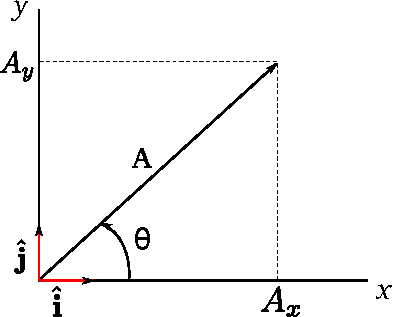
\includegraphics[scale=1]{avec}
  \caption{Vector $\mathbf{A}$}
\label{fig:avec}
\end{figure}


La magnitud al cuadrado del vector se obtiene del teorema de Pitagoras
\begin{align}
  \label{eq:pitagoras}
  \mathbf{A}\cdot\mathbf{A}\equiv|\mathbf{A}|^2=A^2=&A_x^2+A_y^2\nonumber\\
  =&\sum_{i=1}A_i^2\,.
\end{align}
Definiendo el delta de Kronecker como
\begin{align}
  \delta_{ij}=
  \begin{cases}
    1&\text{si $i=j$}\\
    0&\text{si $i\neq j$}\\
  \end{cases}
\end{align}
podemos escribir la magnitud al cuadrado del vector $\mathbf{A}$ de una forma que se puede generalizar facilmente a $n$-dimensiones. Para $n=3$ por ejemplo:
\begin{align}
   A^2=\mathbf{A}\cdot\mathbf{A} =&\sum_{i,j=1}^3A_i A_j\delta_{ij}\nonumber\\
   =&\sum_{i=1}^3\left(A_iA_1\delta_{i1}+A_iA_2\delta_{i2}+A_iA_1\delta_{i3}\right)\nonumber\\
   % falta un paso
   =&A_1A_1\delta_{11}+A_2A_2\delta_{22}+A_3A_3\delta_{33}\nonumber\\
   =&A_1^2+A_2^2+A_3^2\nonumber\\
   =&\sum_{i=1}^3A_i^2\,.
\end{align}
Teniendo en cuenta el \'angulo $\theta$ definido en la figura \ref{fig:avec} en la ec.\eqref{eq:pitagoras}, tenemos que
\begin{align}
  A_x=&|\mathbf{A}|\cos\theta=A\cos\theta\nonumber\\
  A_y=&|\mathbf{A}|\sin\theta=A\sin\theta\,,
\end{align}
De modo que
\begin{align}
  \tan\theta=\frac{A_y}{A_x}\,,
\end{align}
y
\begin{align}
  \theta=\tan^{-1}\frac{A_y}{A_x}
\end{align}


\subsection{Vectores y escalares}


Una cantidad que es representada por un sólo número es llamada un \emph{escalar} \cite{MI}. Una cantidad escalar no tiene dirección, Ejemplos incluyen la masa de un objeto, tal como uno de 5~Kg. o una tempetatura tal como $-20^\circ\ $C. Vectores y escalares son entidades muy diferentes; un vector nunca puede ser igual a un escalar, y un escalar no se pude sumar a un vector. Los escalares pueden ser positivos o negativos:
\begin{align*}
  m=&50\ \text{Kg}\\
  T=&-20^\circ\ \text{C} 
\end{align*}

Aunque una componente de un vector tal como $A_x$ no es un vector, tampoco es un escalar, a pesar de ser sólo un número. Una propiedad muy importante de un escalar es que este no cambia si cambiamos el sistema de referencia, mientras que la componente de un vector si puede cambiar, por ejemplo si orientamos los ejes de coordenadas $x, y, z$ de una forma diferente.


\subsection{Operaciones vectoriales}

Para sumar dos vectores algebra\'\i camente, se desplazan los origenes de los dos vectores a un origen de coordenadas que coincida con el plano formado por los dos vectores, como se muestra en la figura~\ref{fig:apbvec}. Entonces es facil ver que
\begin{align}
  \mathbf{C}=\mathbf{A}+\mathbf{B}=&(A_x+B_x)\hat{\mathbf{i}}+(A_y+B_y)\hat{\mathbf{j}}\nonumber\\
  =&(A_x+B_x,A_y+B_y)\nonumber\\
  =&(A_1+B_1,A_1+B_1).
\end{align}

\begin{figure}
  \centering
  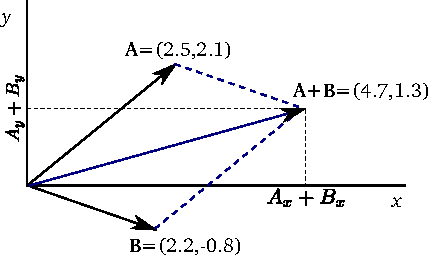
\includegraphics[scale=1]{apbvec}
  \caption{Suma algebráica de vectores}
\label{fig:apbvec}
\end{figure}
En t\'erminos de componentes:
\begin{align}
  \left(\mathbf{A}+\mathbf{B}\right)_i=A_i+B_i\,.
\end{align}
\end{frame}

%Ejemplo sonbre descomposición del peso en un plano inclinado

\begin{figure}
  \centering
  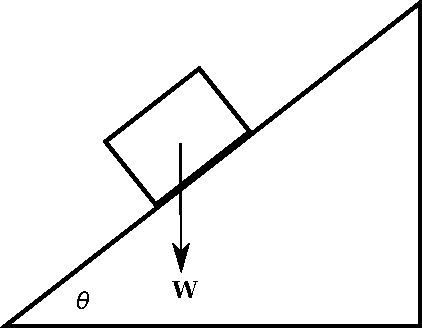
\includegraphics{planopeso1}
  \caption{Peso}
  \label{fig:planopeso1}
\end{figure}

\begin{figure}
  \centering
  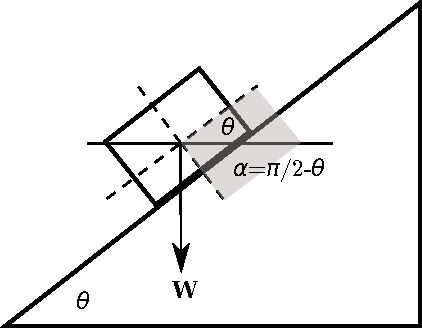
\includegraphics{planopeso2} 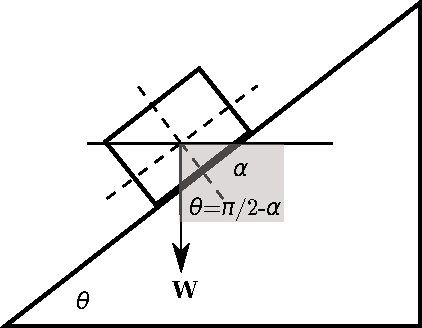
\includegraphics{planopeso3} 
  \caption{Peso}
  \label{fig:planopeso2}
\end{figure}

\begin{frame}[fragile,allowframebreaks]
Procedemos ahora a definir el \emph{producto escalar entre dos vectores} cuyo resultado es un escalar como:
\begin{align}
  \mathbf{A}\cdot\mathbf{B}\equiv&A_xB_x+A_yB_y\nonumber\\
  =&\sum_{i,j=1}^2A_iB_j\delta_{ij}\nonumber\\
  =&\sum_{i}^2A_iB_i\,,
\end{align}

El producto escalar puede escribirse en términos de la magnitud de los
vectores y el ángulo entre ellos. Para ello definimos $\beta$ como el
\'angulo entre los vectores $\mathbf{A}$ y $\mathbf{B}$. Escojemos el
sistema de coordenadas en el plano formado por los dos vectores tales
que $\alpha+\beta$ sea el \'angulo de $\mathbf{A}$ con $x$ y $\alpha$
el \'angulo de $\mathbf{B}$, como se mueste en la figura~\ref{fig:adotbvec}. 

\begin{figure}
  \centering
  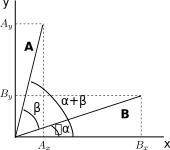
\includegraphics[scale=1]{adotbvec}
  \caption{Producto escalar entre dos vectores}
  \label{fig:adotbvec}
\end{figure}

Entonces, de la definici\'on tenemos:
\begin{align}
    \mathbf{A}\cdot\mathbf{B}=&A_xB_x+A_yB_y\nonumber\\
    =&A\cos(\alpha+\beta)B\cos\alpha+A\sin(\alpha+\beta)B\sin\alpha\nonumber\\
    =&AB[(\cos\alpha\cos\beta-\sin\alpha\sin\beta)\cos\alpha+(\sin\alpha\cos\beta+\cos\alpha\sin\beta)\sin\alpha]\nonumber\\
    =&AB(\cos^2\alpha+\sin^2\alpha)\cos\beta\nonumber\\
    =&AB\cos\beta\nonumber\\
    =&|\mathbf{A}||\mathbf{B}|\cos\beta\,,
\end{align}
De este modo, el \'angulo entre dos vectores,
$\beta$, se puede obtener como
\begin{align}
  \cos\beta=\frac{\mathbf{A}\cdot\mathbf{B}}{|\mathbf{A}||\mathbf{B}|}\,.
\end{align}
\end{frame}

%ejemplo trabajo

\begin{frame}[fragile,allowframebreaks]
El producto vectorial $\mathbf{C}=\mathbf{A}\timesm\mathbf{B}$, se define algebra\'\i camente como:
\begin{align}
  C_k=\left(\mathbf{A}\timesm\mathbf{B}\right)_k=&\sum_{ij}\epsilon_{ijk}A_iB_j\,,
\end{align}
donde el s\'\i mbolo de Levi-Civita se define con respecto a las
permutaciones con referencia al orden 123 como
\begin{align}
  \epsilon_{ijk}\equiv& \begin{cases}
    0&\text{si hay \'\i ndices iguales}\\
    1&\text{permutaci\'on par}\\
    -1&\text{permutaci\'on impar}\\
  \end{cases}.
\end{align}
Entonces
\begin{align}
  C_x=C_1=\left(\mathbf{A}\timesm\mathbf{B}\right)_1=&
\sum_{i=1}^3\left(\cancel{\epsilon_{i11}}A_iB_1+\epsilon_{i21}A_iB_2+\epsilon_{i31}A_iB_3\right)\nonumber\\
=&\cancel{\epsilon_{121}}A_1B_2+\cancel{\epsilon_{221}}A_2B_2
+\epsilon_{321}A_3B_2+\cancel{\epsilon_{131}}A_1B_3\nonumber\\
&+\epsilon_{231}A_2B_3+\cancel{\epsilon_{331}}A_3B_3\,.
\end{align}
Teniendo en cuenta que $321\to231\to213\to123$ (3 permutaciones) y
$231\to213\to123$ (2 permutaciones), entonces
\begin{align}
  \epsilon_{321}=-1\,\qquad \epsilon_{231}=+1\,,
\end{align}
de modo que
\begin{align}
  C_x=C_1=&A_2B_3-A_3B_2\,.
\end{align}
Similarmente para $C_y$ y $C_z$, tenemos
%faltan detalles
\begin{align}
  \label{eq:crossprod}
  \mathbf{C}=&\left(A_yB_z-A_zB_y\right)\hat{\mathbf{i}}
-\left(A_xB_z-A_zB_x\right)\hat{\mathbf{j}}
+\left(A_xB_y-A_yB_x\right)\hat{\mathbf{k}}\nonumber\\
 =&\left(A_2B_3-A_3B_2,A_3B_1-A_1B_3,A_1B_2-A_2B_1\right)
\,.
\end{align}
Definimos
\begin{align}
  \label{eq:det}
  \mathbf{C}=\begin{vmatrix}
    \hat{\mathbf{i}} & \hat{\mathbf{j}} & \hat{\mathbf{k}}\\
    A_x & A_y & A_z\\
    B_x & B_y & B_z
  \end{vmatrix}\equiv\left(A_yB_z-A_zB_y\right)\hat{\mathbf{i}}
-\left(A_xB_z-A_zB_x\right)\hat{\mathbf{j}}
+\left(A_xB_y-A_yB_x\right)\hat{\mathbf{k}}\,.
\end{align}
El resultado (\ref{eq:crossprod}) se puede obtener tambi\'en con la
regla para calcular el determinante definido en la ec.~(\ref{eq:det}),
como se muestra en la figura~\ref{fig:cross}.
\begin{figure}
  \centering
  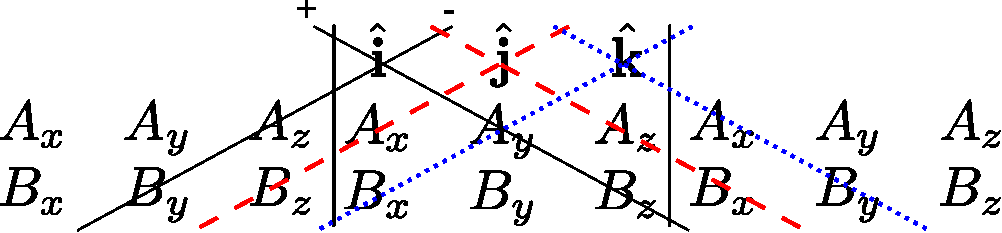
\includegraphics[scale=0.7]{cross}
  \caption{Regla para el determinante: Para cada par de l\'\i neas, el cruze de las l\'\i neas definen
    el vector unitario, que va acompa\~nado por el producto de las
    cantidades bajo la l\'\i nea de izquierda  a derecha menos el producto
    de la cantidades de derecha a izquierda. El signo menos aparece
    naturalmente para el producto asociado a $\hat{\mathbf{j}}$.  }
  \label{fig:cross}
\end{figure}

Para mostrar como el producto vectorial se reduce la definici\'on
geom\'etrica en t\'erminos de las magnitudes y el \'angulo entre los dos
vectores, considere el plano definido por los vectores $\mathbf{A}$ y
$\mathbf{B}$ que forman un \'angulo $\alpha$ entre ellos. Escojamos el eje
$x$ a lo largo del vector $\mathbf{A}$, como se muestra en la en la figura~\ref{fig:axbvec}. 

\begin{figure}
  \centering
  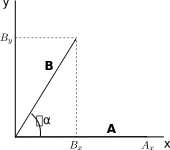
\includegraphics[scale=1]{axbvec}
  \caption{Producto escalar entre dos vectores}
  \label{fig:axbvec}
\end{figure} 

Entonces:
\begin{align}
  A_y=A_z=B_z=0\qquad A=A_x\qquad\text{y}\ B_y=B\sin\alpha\,. 
\end{align}
Por consiguiente
\begin{align}
  \mathbf{C}=\mathbf{A}\timesm\mathbf{B}=&A_xB_y\hat{\mathbf{k}}\nonumber\\
  =&A B\sin\alpha\,\hat{\mathbf{k}}\,,
\end{align}
y entonces
\begin{align}
  |\mathbf{C}|=|\mathbf{A}||\mathbf{B}|\sin\alpha\,.
\end{align}
\end{frame}

\begin{itemize}
\item[\textbf{Ejemplo:}] Sea $\mathbf{r}$ la distacia desde algún punto sobre la vertical de un círculo de radio $R$ hasta su punto más inferior: $P$, como se ilustra en la figura~\ref{fig:examplecross}. Calcule el producto escalar entre $\mathbf{r}$ y $\mathbf{f}$ cuando el punto sobre (a) la vertical está en en el centro del círculo ($C$),  (b) cuando está en el punto inferior $P$ y (c) cuando está en el punto superior. Índique claramente la dirección del vector resultante. Si $\mathbf{f}$ es una fuerza índique además el sentido del giro del círculo con un eje pasando por su centro.
  \begin{figure}
    \centering
    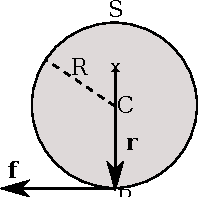
\includegraphics{examplecross}
    \caption{Ejemplo productor vectorial}
    \label{fig:examplecross}
  \end{figure}

\textbf{Solución:} Para el eje $z$ saliendo de la página (a) $\mathbf{r}\times\mathbf{f}=-R f \hat{\mathbf{k}} $, dirección horaria de giro (b) $\mathbf{r}\times\mathbf{f}=\mathbf{0}\times\mathbf{f}=\mathbf{0}$ y (c) $\mathbf{r}\times\mathbf{f}=-2R f \hat{\mathbf{k}} $, dirección horaria de giro.

\end{itemize}

\subsection{Cambio en una cantidad}

Frecuentemente queremos calcular el cambio en una cantidad. Por
ejemplo, podríamos desear conocer el cambio en la posición de un
objeto en movimiento, o el cambio en la velocidad durante un intervalo
de tiempo. La letra $\Delta$ (delta mayúscula que sugiere una ``$d$ de
diferencia'') se usa para denotar el cambio en una cantidad ya sea
escalar o vectorial.

%\begin{extrapage}
%  \newpage
  
%  \qquad
%  \newpage
%\end{extrapage}

%%% Local Variables: 
%%% mode: latex
%%% TeX-master: "mecanica"
%%% End:

\chapter{Interacciones y movimiento}

 
\section{Diagramas mostrando cambios de velocidad}

Está parte de la notas está basada en el libro Matter \& Interactions \cite{MI}

En diagrámas físicaos la velocidad de un objeto es representada por un
vector: una línea con una flecha. La cola de la flecha se coloca donde
el objeto está localizado, y la punta de la flecha en la dirección del
movimiento del objeto. La longitud de la flecha es proporcional a la
velocidad del objeto. De este modo la velocidad se describe como un
vector. A la magnitud de la velocidad se le llama rapidez.

\subsection{Movimiento uniforme}
Suponga que observa una roca moviéndose en el espacio exterior
bastante alejada de cualquier objeto. No sabemos que la hizo mover la
primera vez; presumiblemente hace mucho tiempo una interacción le dio
alguna velocidad y esta ha estado moviéndose desde entonces en el
espacio vacio.

Es un hecho observacional que tal objeto aislado se mueve con una
rapidez constante (que no cambia), en una línea recta. Su velocidad no
cambia (ni su dirección ni su rapidez
\begin{figure}
  \centering
  \includegraphics[scale=0.2]{uniform}
  \caption{Movimiento uniforme: sin cambio en la rapidez o la dirección.}
  \label{fig:uniform}
\end{figure}
cambia). A tal movimiento con
velocidad constante le llamaremos movimiento uniforme y es ilustrado
en la figura~\ref{fig:uniform}

Si observamos un electrón cambiando la dirección de su velocidad, podemos atribuirlo al efecto de repulsión de un electrón cercano como se muestra en la figura~\ref{fig:repulsion2} (a). Mientras que si el electrón se está acelerando en línea recta, cambiando la magnitud de su velocidad pero manteniendo la dirección, lo podemos atribuir a otro electrón a lo largo de su línea de movimiento como se muestra en la figura~\ref{fig:repulsion2} (b)
\begin{figure}
  \centering
  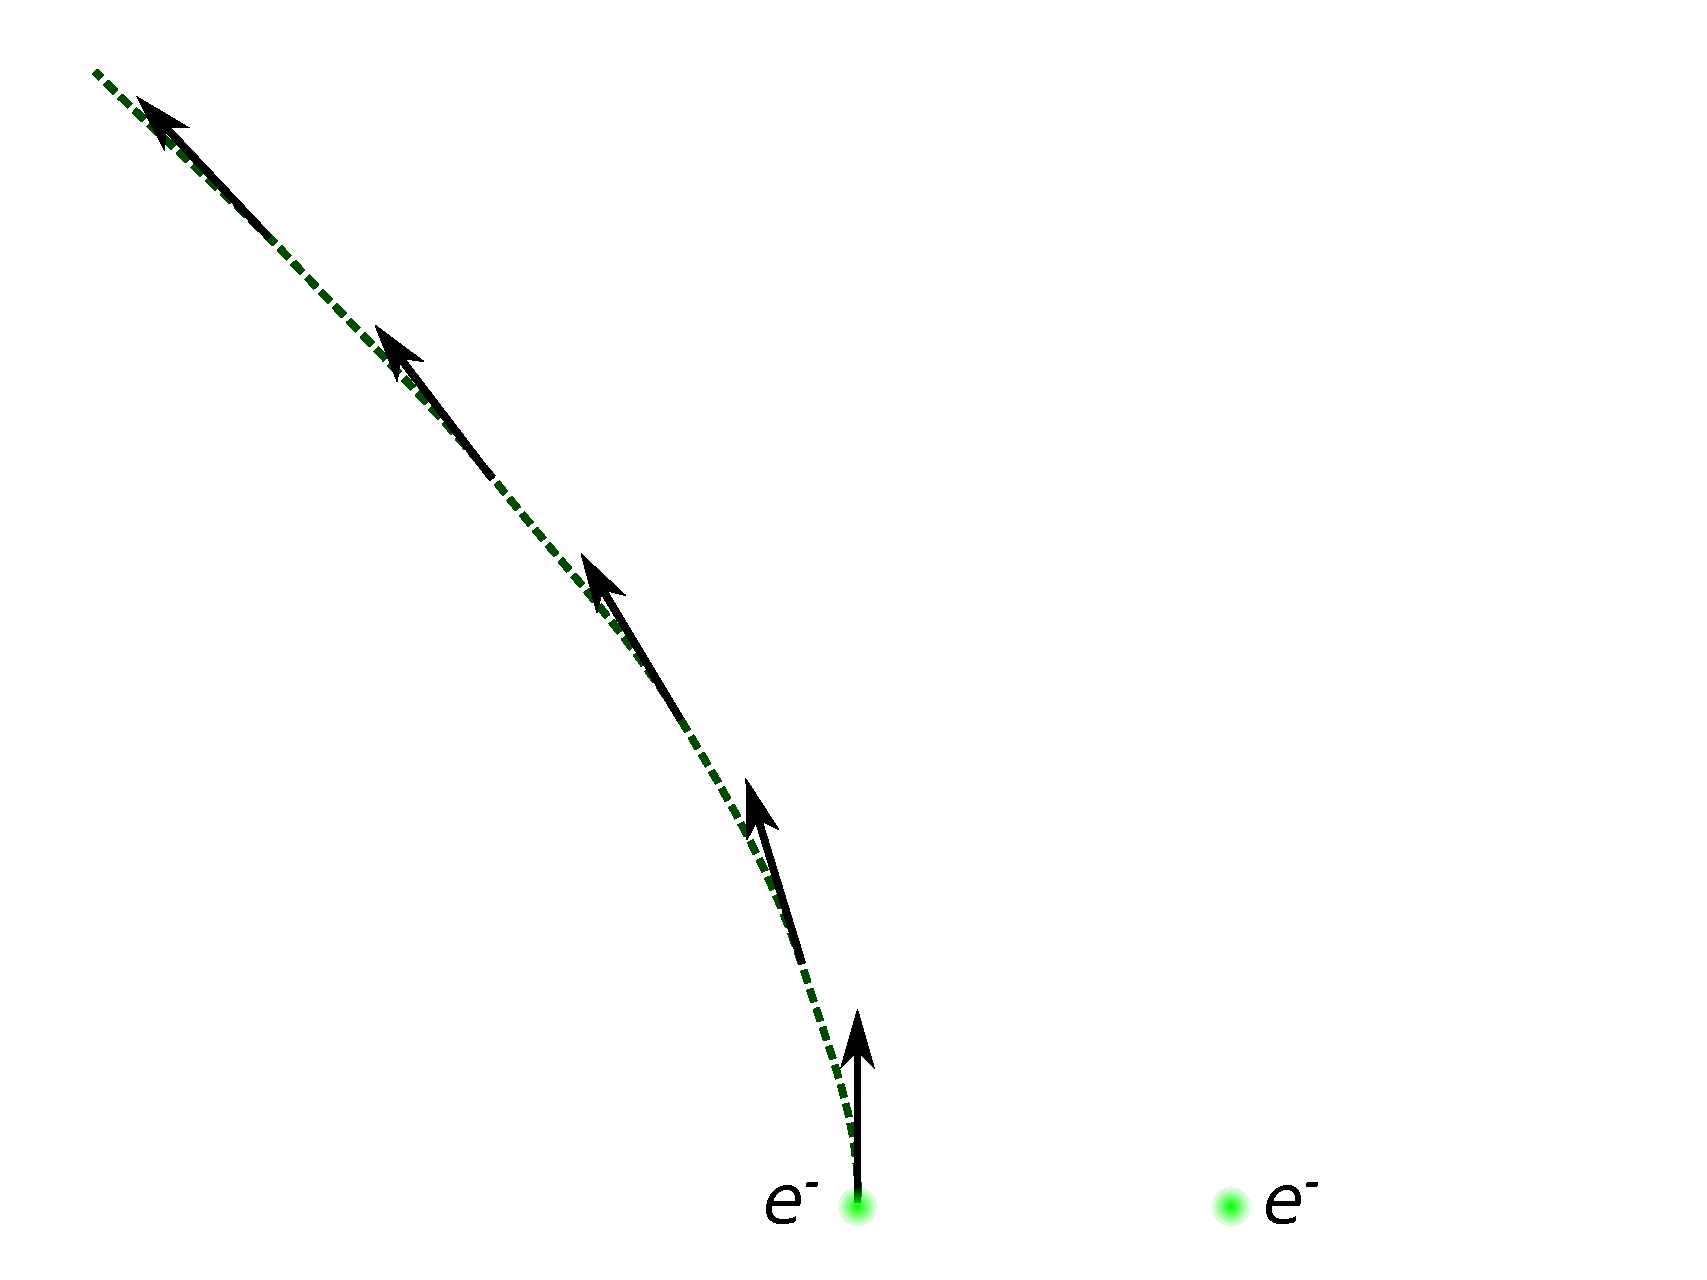
\includegraphics[scale=0.3]{repulsion2} 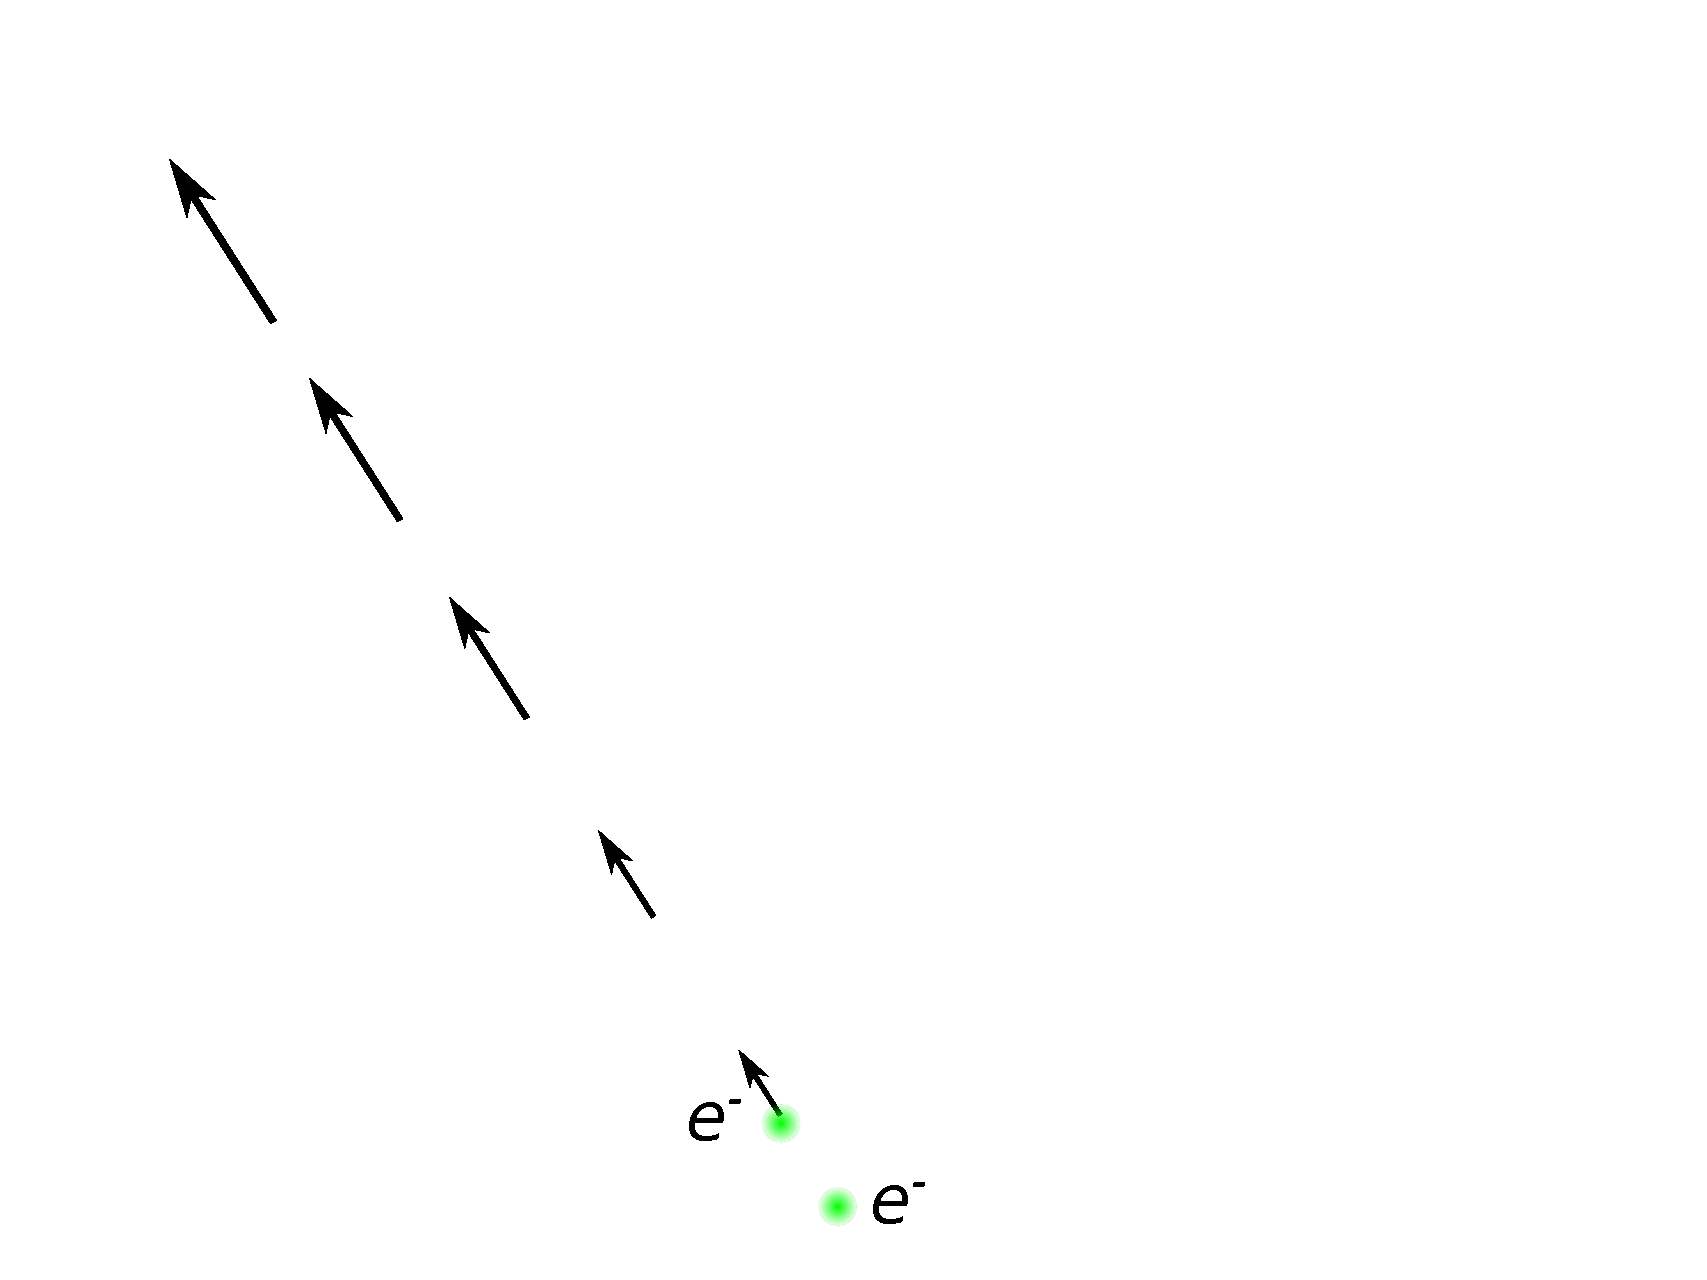
\includegraphics[scale=0.3]{repulsion4}\\
    (a) \hspace{5cm} (b)
  \caption{Cambio en dirección}
  \label{fig:repulsion2}
\end{figure}

Podemos establecer entonces,

\begin{frame}
  \begin{block}{Primera Ley de Newton:}
    Un objeto se mueve en línea recta y a una rapidez constante
    excepto en la medida que interactue con otros objetos
  \end{block}
\end{frame}

Antes de la Primera Ley de Newton,  se pensaba que se requería un empuje constante para mantener algo en movimiento. Con La Primera Ley de Newton, o Ley de Inercia, ¡No se necesitan interacciones para que algo se mueva! (o, como veremos luego, rote)


Para mantener una silla moviéndose a velocidad constante hay que estar empujándola todo el tiempo. La primera Ley de Newton ¿implicaría que la silla se debe mover a velocidad constante sin que nadie la esté empujando? ¿El empuje constante debería cambiar la dirección o la rapidez del movimiento? ¿está situación de la vida diaria viola la primera ley de Newton?

El factor que complica la situación es que sus manos no son lo único que interacciona con la silla. El piso también interacciona con la silla en una forma que llamamos fricción. Si se empuja la silla lo suficiente como para compensar \emph{exactamente} la fricción, la suma total de las interacciones es \emph{cero}, y la silla se mueve a velocidad constante como lo predice la primera ley de Newton. Si el empuje es más fuera que la fuerza que hace el piso, entonces la rapidez de la silla se debe incrementar.


Es muy difícil observar movimiento sin fricción en la vida diaria, debido a que los objetos interaccionan con otros objetos incluyendo el aire, superficies, etc. Esto explica porque le tomo a la gente tanto tiempo entender claramente la relación entre interacción y cambio (Newton nación en 1942).

\begin{frame}
Ejemplos de baja fricción
\begin{itemize}
\item Un disco de hockey deslizándose sobre el hielo.
\item Un tren sobre los rieles de acero.
\item Un tren de levitación magnético a bajas velocidades.
\item Un tren de levitación magnético moviéndose a lo largo de un tubo de vacío.
\item Un objeto en el espacio exterior lejos de cualquier objeto.
\end{itemize}
\end{frame}


\begin{frame}
  De acuerdo a la primer ley de Newton, cuales de las siguientes frases sobre el movimiento de una nave después de apagada son correctas
  \begin{enumerate}
  \item La nave se moverá en línea recta
    \label{item:n1}
  \item La nave viajará en una trayectoria curva
  \item La nave entrará en una orbita circular
  \item La velocidad de la nave no cambiará
    \label{item:n2}
  \item La nave se detendrá gradualmente
  \item La nave parará de inmediato
  \end{enumerate}
\end{frame}

La \ref{item:n1}. y la \ref{item:n2}.

La humanidad tardó aún mucho más tiempo en determinar cuales de las fuerzas en la naturaleza eran fundamentales y cuales eran simplemente resultaban por el efecto combinando de interacciones fundamentales.

Hoy sabemos que en la naturaleza existen cuatro interacciones fundamentales
\begin{itemize}
\item Interacción gravitacional.
\item Interacción electromagnética.
\item Interacción débil.
\item Interacción fuerte.
\end{itemize}

Las demás fuerzas como la fuerza nuclear, la fuerzas de Van der Waals, la fricción, la viscosidad, etc., son remanentes de la interacciones fundamentales. 

%Ver presentación sobre Interacciones y movimiento donde se establece la Primera Ley de Newton en la página del curso.

\section{Velocidad}

\subsection{Rapidez promedio}
La rapidez es la magnitud del vector velocidad  y por consiguiente es una cantidad escalar:

\begin{align}
  \label{eq:27}
\bar{v}=\frac{d}{t}\,,
\end{align}
donde $\bar{v}$ es la \emph{rapidez promedio}, $d$ es la distancia
recorrida durante un tiempo $t$. En SI (Système Internationale) de
unidades, la rapidez promedio se mide en metros por segundo, y se
abrevia con $\meter\per\second$.

De \eqref{eq:27}
\begin{align}
  \label{eq:26}
  d=&\bar{v} t\nonumber\\
  t=&\frac{d}{\bar{v}}\,.
\end{align}

Es importante notar que las ecuaciones \eqref{eq:26} son dimensionalmente correctas, por ejemplo
\begin{align}
  [d]=&  \left[\bar{v}   \right] [t]\nonumber\\
  L=&\frac{L}{T}\times T\nonumber\\
  L=&L\,.
\end{align}

\subsection{Rapidez instantanea comparada a rapidez promedio}

Si un carro se mueve a $70\ \text{Km/h}$ (Kilometros por hora) durante la primera hora y a $30\kilo\meter\per\hour$
durante la segunda hora, este recorre en total 100~Km en 2 horas, con una rapidez promedio
\begin{align}
  \bar{v}=\frac{100\kilo\meter}{2\hour}=50\kilo\meter\per\hour\,.
\end{align}
Note que durante el intervalo de dos horas el carro nunca estuvo viajando realmente a su rapidez promedio de $50\kilo\meter\per\hour$.

El movimiento es ilustrado en un gráfico de distancia contra tiempo en la figura~\ref{fig:vinstaprom3} (detalles en la presentación \href{http://goo.gl/3eqUa}{aquí})

\begin{frame}[plain]
\begin{figure}
  \centering
  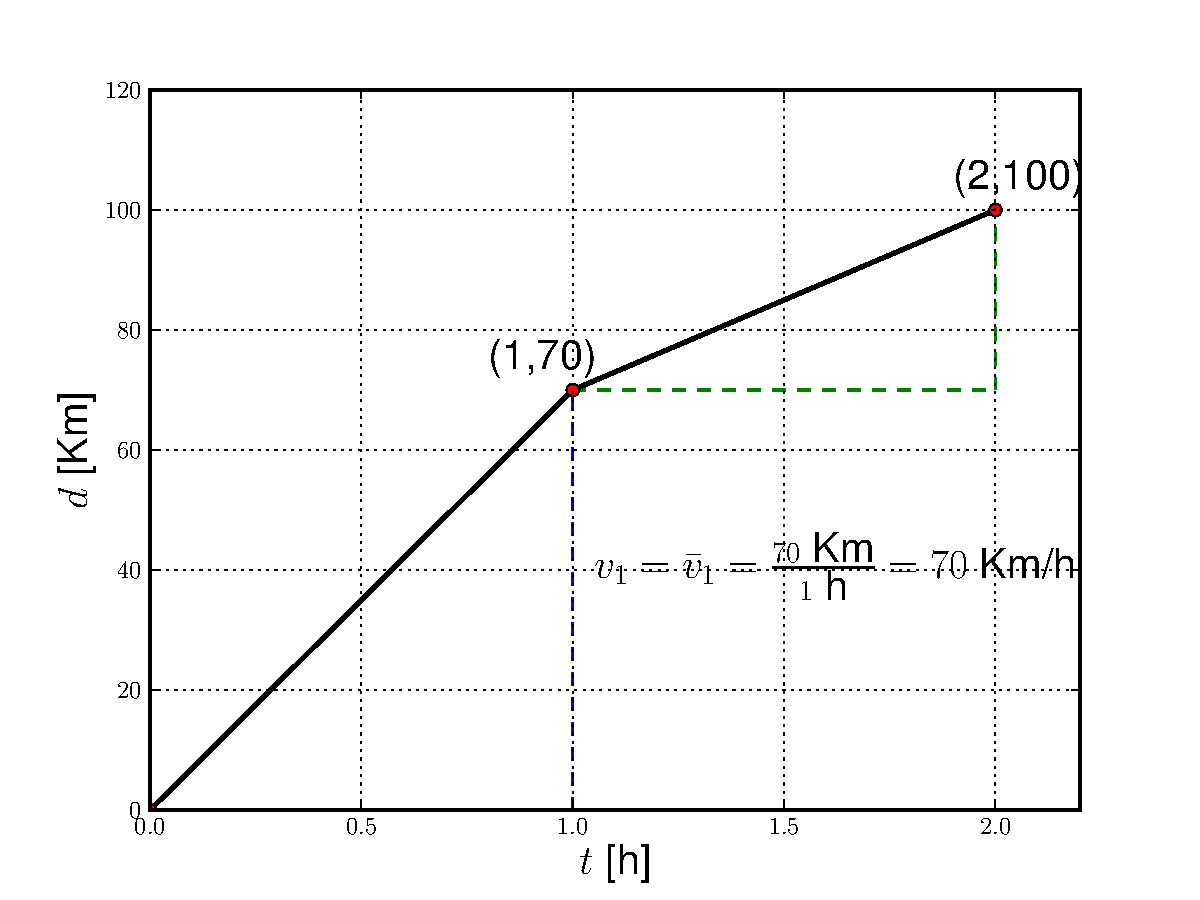
\includegraphics[scale=0.6]{vinstaprom3}
  \caption{Gráfico de distancia versus tiempo}
  \label{fig:vinstaprom3}
\end{figure}
\end{frame}


La rapidez instantánea es la rapidez del carro en un instante particular. Para encontrarla debemos observar una distancia corta en la que el carro se mueva en un intervalo de tiempo muy corto, digamos que una centesima de segundo. Si durante algún momento de la segunda hora el carro se mueve 0.0833 metros en 0.01 segundos, su rapidez instantanea es:
\begin{align}
  v=0.0833/0.01=8.33 \meter\per\second\,,
\end{align}
que en \kilo\meter\per\hour\ corresponde a
\begin{align}
  v=8.33\ \frac{\cancel{\meter}}{\cancel{\second}}\frac{3600\ \cancel{\second}}{1\hour}\frac{1\ \kilo\meter}{1000\ \cancel{\meter}}=30\kilo\meter\per\hour\,.
\end{align}

En el caso que se ilustra en la figura~\ref{fig:vinstaprom3}

\section{Movimiento en varias dimensiones}

\subsection{Vector de Posición}
Nuestra segunda aplicaci\'on de vectores ser\'a la descripci\'on  de la posici\'on y movimiento de un punto en el espacio en tres dimensiones. 

La posici\'on de un punto en el espacio: $(x_1,y_1,z_1)$ no representa un vector. Sin embargo, si movemos el punto a alguna nueva posici\'on, $(x_2,y_2,z_2)$, entonces el desplazamiento define un vector 
\begin{align}
  \Delta \mathbf{r}=\mathbf{r}_2-\mathbf{r}_1
\end{align}
$\Delta\mathbf{r}$ significa ``cambio de $\mathbf{r}$'' o $\mathbf{r}_2-\mathbf{r}_1$ (desplazamiento)

$\Delta t$ significa ``cambio de $t$'' or $t_2-t_1$ (intervalo de tiempo)

El símbolo $\Delta$ (delta) siempre significa ``final menos inicial''

\begin{align}
  \Delta\mathbf{r}=(x_2-x_1,y_2-y_1,z_2-z_1)\,.
\end{align}
$\Delta\mathbf{r}$ es un vector verdadero, aunque los valores de la coordenadas inicial y final dependen del sistema de coordenadas, $\Delta\mathbf{r}$ no depende del sistema de coordenadas. 

$\Delta\mathbf{r}$ tiene las dimensiones f\'\i sicas de longitud. 

%hablar de un ejemplo concreto como el de la abeja de MI Fig. 1.31

El vector de desplazamiento apunta desde la posición inicial hacia la posición final (final menos inicial).

%calcular el desplazamiento númerico de la abeja

Aunque los vectores definen desplazamientos en lugar de posiciones, es posible describir la posici\'on de un punto con respecto al origen de un sistema de coordenadas dado por un vector especial, conocido como el \emph{vector de posici\'on}, que se extiende desde el origen hasta el punto de inter\'es. Usaremos el s\'\i mbolo $\mathbf{r}$ para denotar el vector de posici\'on. La posici\'on de un punto arbitrario $P$ se escribe como
\begin{align}
  \mathbf{r}=(x,y,z)=x\hat{\mathbf{i}}+
  y\hat{\mathbf{j}}+z\hat{\mathbf{k}}\,.
\end{align}

A diferencia de los vectores ordinarios, $\mathbf{r}$ depende del sistema de coordenadas. Si $\mathbf{R}$ es el vector desde el origen de un sistema de coordenadas no primado al origen de un sistema de coordenadas primado, tenemos
\begin{inprogress}
  Escribir los detalles...
\end{inprogress}
\begin{align}
  \mathbf{r}'=\mathbf{r}-\mathbf{R}\,.
\end{align}
Un verdadero  vector es independiente del sistema de coordenadas. Como se muestra en la figura~\ref{fig:vpos},
\begin{align}
  \Delta\mathbf{r}=&\mathbf{r}_2-\mathbf{r}_1\nonumber\\
  =&\mathbf{\mathbf{r}_2'+\mathbf{R}}
-\mathbf{\mathbf{r}_1'+\mathbf{R}}\nonumber\\
=&\mathbf{r}_2'-\mathbf{r}'_1\,.
\end{align}
\begin{frame}[plain]
  \begin{figure}
  \centering
  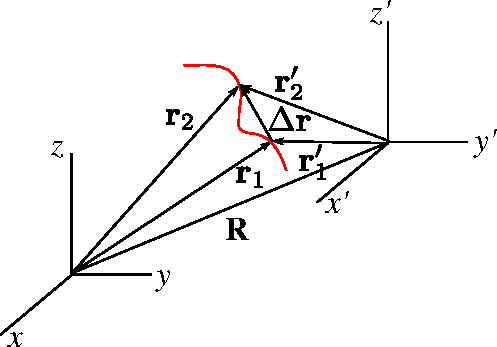
\includegraphics[scale=0.85]{deltar3d}
  \caption{Vector de desplazamiento. (Sec 1.6 \cite{Kleppner})}
  \label{fig:vpos}
\end{figure}
\end{frame}

\subsection{Determinando la velocidad promedio desde un cambio en la posición}
La posici\'on instant\'anea de una part\'\i cula a un tiempo $t_i$ es
\begin{align}
  \mathbf{r}(t_1)=(x(t_1),y(t_1),z(t_1))\qquad \text{\'o}\qquad
  \mathbf{r}_1=(x_1,y_1,z_1)\,,
\end{align}
donde $x_1$ es el valor de $x$ en $t=t_1$, y as\'\i{} sucesivamente. Al tiempo $t_2$ la posici\'on es
\begin{align}
  \mathbf{r}_2=(x_2,y_2,z_2)\,.
\end{align}
El desplazamiento de la part\'\i cula entre los tiempos $t_1$ y $t_2$ es
\begin{align}
  \mathbf{r}_2-\mathbf{r}_1=(x_2-x_1,y_2-y_1,z_2-z_1)\,.
\end{align}



\begin{inprogress}
Pasar las notas del cuaderno de MI aquí.

Escribir los detalles %t_1=t Delta t=t_2-t-> t_2=t+Delta t
\end{inprogress}
El desplazamiento de una part\'\i cula entre los tiempos $t$ y un tiempo posterior $t+\Delta t$ es
\begin{align}
  \Delta\mathbf{r}=\mathbf{r}(t+\Delta t)-\mathbf{r}(t)\,.
\end{align}


\begin{inprogress}
  Fig pag 15 of Kleppner.
\end{inprogress}

\begin{itemize}
\item[Ejemplo]: En dos dimensiones, esta ecuaci\'on es equivalente a
  \begin{align}
    \Delta x=&x(t+\Delta t)-x(t)\nonumber\\
    \Delta y=&y(t+\Delta t)-y(t)\,.
  \end{align}
  como se muestra en la figura~\ref{fig:deltar}
  \begin{figure}
    \centering
    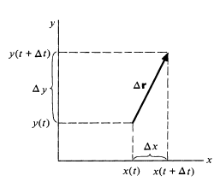
\includegraphics[scale=0.55]{deltar}
    \caption{Desplazamieto entre $t_1$ y $t_2$ (Sec 1.6~\cite{Kleppner})}
    \label{fig:deltar}
  \end{figure}

\end{itemize}


\begin{itemize}
\item[\textbf{Ejemplo:}] Considere una abeja volando. En un tiempo inicial el vector de posición de la abeja es
  \begin{align}
    \mathbf{r}_i=(2,4,0)\meter,\qquad t_i=0\,,
  \end{align}
$0.1\second$ después, la posición es
\begin{align}
  \mathbf{r}_f=(3,3.5,0)\meter,\qquad t_f=0.1\second\,.
\end{align}
Realice un diagrama de la situación y encuentre
\begin{enumerate}
\item la velocidad promedio
  \label{item:abejaa}
\item La rapidez promedio
  \label{item:abejab}
\item La dirección de la velocidad promedio
  \label{item:abejac}
\end{enumerate}
\begin{itemize}
\item[\ref{item:abejaa}.] 

\begin{align*}
  \mathbf{v}_{\text{prom}}=(10,-5,0)\meter\per\second\,.
\end{align*}

\item[\ref{item:abejab}.]
\begin{align*}
  v_{\text{prom}}=11.18\meter\per\second\,.
\end{align*}
\item[\ref{item:abejac}.]
  \begin{align*}
    \hat{\mathbf{v}}_{\text{prom}}=\frac{\mathbf{v}_{\text{prom}}}{v_{\text{prom}}}=(0.804,-0.447,0)
  \end{align*}

\end{itemize}
\end{itemize}

\subsection{Velocidad instantánea}

Considere la curva en la figura \ref{fig:flyingball1a}. Los punto de color rojo marcan la posición de una bola a intervalos de tiempo de un segundo. Mientras que la bola está en el aire, su velocidad está constantemente cambiando, debido a las interacciones con la tierra (gravedad) y con el aire (resistencia del aire). 
\begin{figure}
  \centering
  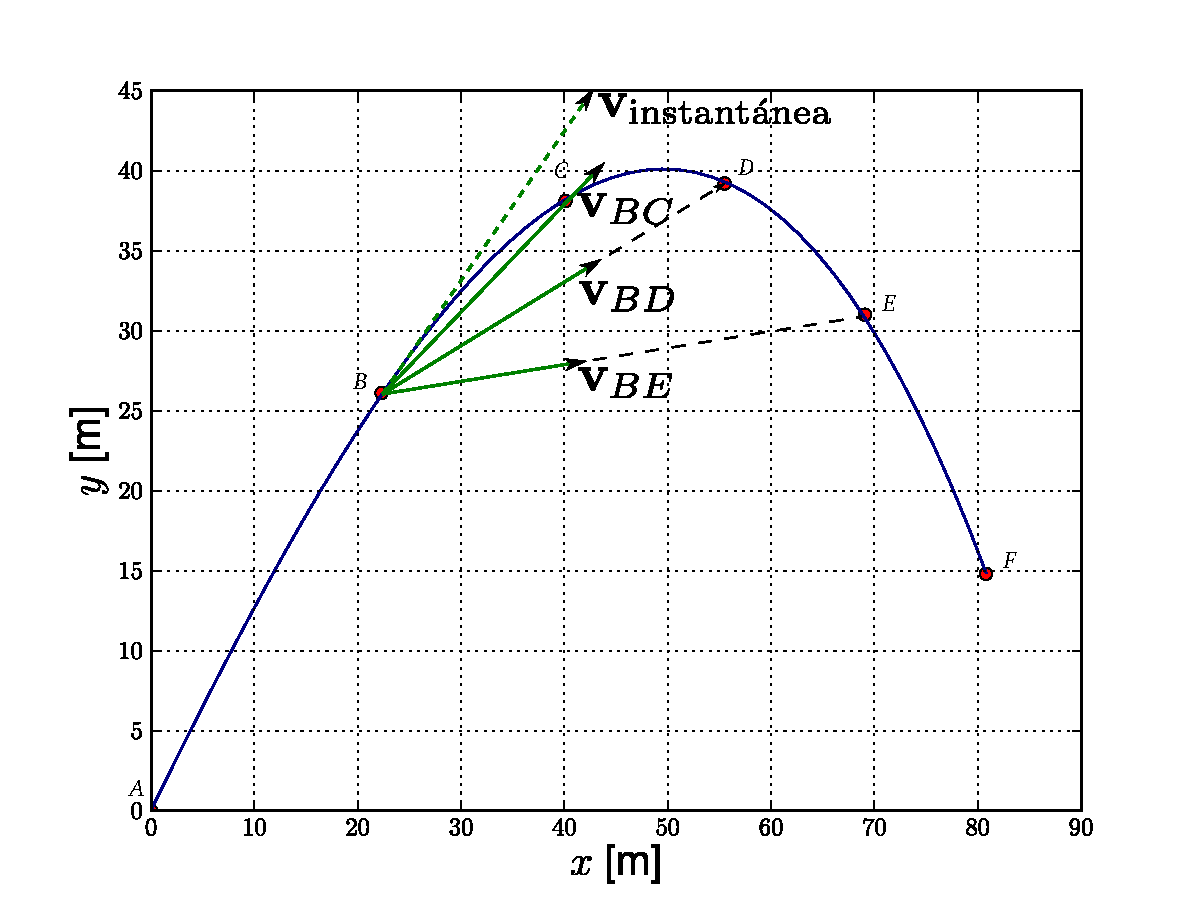
\includegraphics[scale=0.4]{flyingball1a}
  \caption{Movimiento de una bola}
  \label{fig:flyingball1a}
\end{figure}

Suponga que hacemos la pregunta: ¿cual es el valor de la velocidad en el instante preciso que alcanza el punto $B$?. Está cantidad debería llamarse la velocidad instantánea. Podemos aproximar la velocidad instantánea de la bola, encontrando su velocidad promedio sobre un intervalo de tiempo más grande. 

La Tabla muestra el vector de posición de la bola a diferentes tiempos en los puntos ilustrados en la figura~\ref{fig:flyingball1a}.

\begin{table}
  \centering
  \begin{tabular}{|l|l|l|}
    loc. & $t\ (\text{s})$ & Posición (m)\\
    $A$ & $0.0$ &$0,0,0$ \\
    $B$ & $1.0$ &$(22.3,26,1,0)$ \\
    $C$ & $2.0$ &$(40.1,38.1,0)$ \\
    $D$ & $3.0$ &$(55.5,39.2,0)$ \\
    $E$ & $4.0$ &$(69.1,31.0,0)$ \\
    $F$ & $5.0$ &$(80.8,14.8,0)$ \\
  \end{tabular}
  \caption{Tabla mostrando el tiempo transcurrido y la posición de la bola en cada posición de la figura~\ref{fig:flyingball1a}}
  \label{tab:flyingball1a}
\end{table}

\begin{align}
  \mathbf{v}_{EB}=&\frac{\Delta \mathbf{r}_{EB}}{\Delta t}
=\frac{\mathbf{\mathbf{r}_E-\mathbf{r}_B}}{t_E-t_B}=
\frac{[(69.1,31.0,0)-(22.3,26,1,0)]\ \text{m}}{(4.0-1.0)\ \text{s}}\nonumber\\
=&(15.6,1.6,0)\ \frac{\text{m}}{\text{s}}\nonumber\\
  \mathbf{v}_{DB}=&\frac{\Delta \mathbf{r}_{DB}}{\Delta t}
=\frac{\mathbf{\mathbf{r}_D-\mathbf{r}_B}}{t_D-t_B}=
\frac{[(55.5,39.2,0)-(22.3,26,1,0)]\ \text{m}}{(3.0-1.0)\ \text{s}}\nonumber\\
=&(16.6,6.55,0)\ \frac{\text{m}}{\text{s}}\nonumber\\
  \mathbf{v}_{CB}=&\frac{\Delta \mathbf{r}_{CB}}{\Delta t}
=\frac{\mathbf{\mathbf{r}_C-\mathbf{r}_B}}{t_C-t_B}=
\frac{[(40.1,38.1,0)-(22.3,26,1,0)]\ \text{m}}{(2.0-1.0)\ \text{s}}\nonumber\\
=&(17.8,12.0,0)\ \frac{\text{m}}{\text{s}}\,,
\end{align}

\begin{align}
  v_{EB}=&15.7\ \frac{\text{m}}{\text{s}}\nonumber\\
  v_{DB}=&17.8\ \frac{\text{m}}{\text{s}}\nonumber\\
  v_{CB}=&21.5\ \frac{\text{m}}{\text{s}}\,,
\end{align}
%mejorar redacción
¿cual aproxima mejor la velocidad instantánea (figura~\ref{fig:flyingball8})?

\begin{figure}
  \centering
  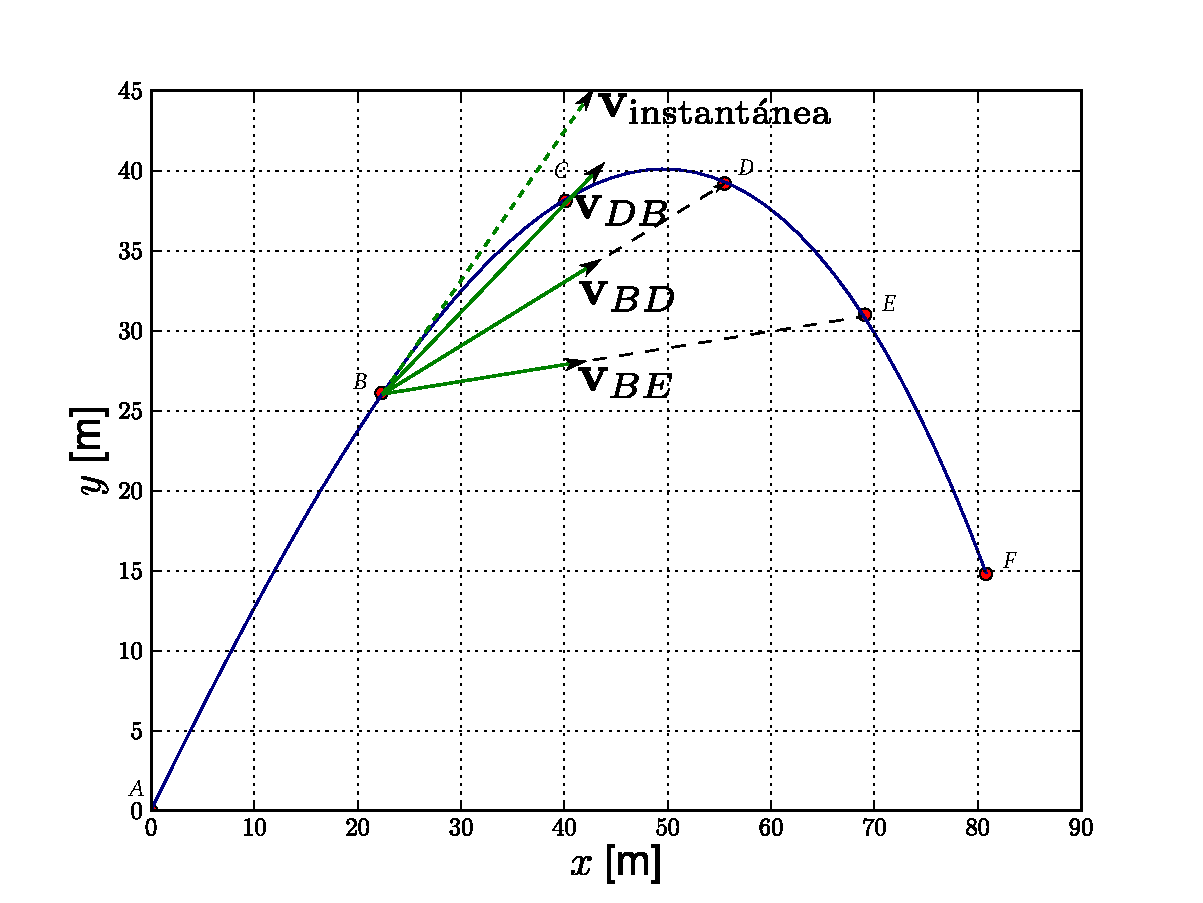
\includegraphics[scale=0.4]{flyingball8}
  \caption{Moviemto de una bola}
  \label{fig:flyingball8}
\end{figure}


La velocidad $\mathbf{v}$ de la partícula a medida que ésta se mueve a lo largo de una trayectoria se define como
\begin{align}
  \mathbf{v}=&\lim_{\Delta t\to0}\frac{\Delta\mathbf{r}}{\Delta t}\nonumber\\
  &=\frac{d\mathbf{r}}{dt}\,,
\end{align}
que es equivalente a las ecuaciones escalares
\begin{align}
  v_x=&\lim_{\Delta t\to0}\frac{\Delta x}{\Delta t}=\frac{dx}{dt}\nonumber\\
  v_y=&\lim_{\Delta t\to0}\frac{\Delta y}{\Delta t}=\frac{dy}{dt}\nonumber\\
  v_z=&\lim_{\Delta t\to0}\frac{\Delta z}{\Delta t}=\frac{dz}{dt}\,.
\end{align}

La notaci\'on vectorial permite describir el movimiento en tres dimensiones con una sola ecuaci\'on, una econom\'\i a muy grande comparada con las tres ecuaciones que tocar\'\i a escribir si se tuviese que hacer de otro modo. 

Alternativamente, ya que $\mathbf{r}=x\hat{\mathbf{i}}+
y\hat{\mathbf{j}}+z\hat{\mathbf{k}}$, obtenemos por simple
diferenciaci\'on que (los vectores unitarios pueden cambiar bajo
diferenciaci\'on en otros sistemas de coordenadas diferentes al
cartesiano)
\begin{align}
 \frac{d\mathbf{r}}{dt}=&\frac{dx}{dt}\hat{\mathbf{i}}   
+\frac{dy}{dt}\hat{\mathbf{j}}   +\frac{dz}{dt}\hat{\mathbf{k}}\nonumber\\
=&
\left(
\frac{dx}{dt},\frac{dy}{dt},\frac{dz}{dt}
\right)\nonumber\\
=&(v_x,v_y,v_z)
\end{align}
%como antes.




En el l\'\i mite $\Delta t\to0$, $\Delta\mathbf{r}$ se convierte en la tangente a la trayectoria, como se \'\i ndica en la figura~\ref{fig:flyingball8}. Sin embargo, la relaci\'on
\begin{align}
  \label{eq:Drvt}
  \Delta\mathbf{r}\approx&\frac{d\mathbf{r}}{dt}\Delta t\nonumber\\
  \Delta\mathbf{r}=&\mathbf{v}\Delta t,
\end{align}
que llega a ser exacta en el l\'\i mite $\Delta t\to 0$, muestra que $\mathbf{v}$ es paralelo a $\Delta\mathbf{r}$; la velocidad instant\'anea $\mathbf{v}$ de una part\'\i cula es en todas partes tangente a la trayectoria. 

%sigue en el cuaderno

La ec.~\eqref{eq:Drvt} puede reescribirse en la forma
\begin{align*}
  \mathbf{r}_2-\mathbf{r}_1=\mathbf{v}_{\text{prom}}(t_2-t_1)\,,
\end{align*}
de modo que el vector de desplazamiento es el promedio del vector de velocidad en el intervalo de tiempo.

Si conocemos la velocidad, tenemos una relación para actualizar la posición a partir de una posición inicial $\mathbf{r}_1$
\begin{align*}
  \mathbf{r}_2=&\mathbf{r}_1+\mathbf{v}_{\text{prom}}(t_2-t_1)\nonumber\\
=&\mathbf{r}_1+\mathbf{v}_{\text{prom}}\Delta t\,.
\end{align*}
Si se conoce la posición inicial, la velocidad promedio y el intervalo temporal, entonces podemos predecir la siguiente posición del movimiento.
\begin{frame}[plain]
  \begin{itemize}
\item[\textbf{Ejemplo:}] A un tiempo $t_1=12.18\second$ después de la 1:30~PM el vector de posición de una bola es $\mathbf{r}_1=(20,8,-12)\meter$ y su velocidad es $\mathbf{v}_{\text{prom}}=(9,-4,6)\meter\per\second$. A un tiempo $t_2=12.21\second$ después de la 1:30~PM: ¿donde está la bola?, asumiendo que la velocidad no cambie en el corto intervalo de tiempo.

  
  \begin{align*}
  \mathbf{r}_2=&\mathbf{r}_1+\mathbf{v}_{\text{prom}}(t_2-t_1)\nonumber\\
  =&(20,8,-12)\meter +  \left[(9,-4,6)\meter\per\second\right](12.21-12-18)\second\nonumber\\
  =&(20,8,-12)\meter+(0.27,-0.12,0.18)\meter\nonumber\\
=&(20.27,7.88,-11.82)\meter\,.
  \end{align*}
\end{itemize}
\end{frame}

\begin{itemize}
\item[Ejemplo] \textbf{Encontrando $\mathbf{v}$ a partir de $\mathbf{r}$}\\
La posici\'on de una part\'\i cula est\'a dada por
\begin{align}
  \mathbf{r}=A(e^{\alpha t}\hat{\mathbf{i}}+e^{-\alpha t}\hat{\mathbf{j}})\,,
\end{align}
donde $\alpha$ es constante. Encuentre la velocidad y bosqueje la trayectoria.
\begin{align}
    \mathbf{v}=&\frac{d\mathbf{r}}{dt}\nonumber\\
    =&A(\alpha e^{\alpha t}\hat{\mathbf{i}}-\alpha e^{-\alpha t}\hat{\mathbf{j}})\,,
\end{align}
o
\begin{align}
  v_x=&A\alpha e^{\alpha t}\nonumber\\
  v_y=&-A\alpha e^{-\alpha t}\,.
\end{align}
La magnitud de $\mathbf{v}$ es
\begin{align}
  v=&\sqrt{v_x^2+v_y^2}\nonumber\\
  =&A\alpha\sqrt{e^{2\alpha t}+e^{-2\alpha t}}\,.
\end{align}

\begin{inprogress}
  Pasar los ejemplo de MI desarrollados en el cuaderno
\end{inprogress}
Al describir el movimiento de un punto, es usualmente útil considerar los casos l\'\i mite:
\end{itemize}

\subsection{Aceleración}

Aceleración promedio:
\begin{align}
  \mathbf{a}_{\text{prom}}=&\frac{\Delta \mathbf{v}}{\Delta t}
\end{align}

Aceleración instantánea
\begin{align}
  \mathbf{a}=&\lim_{\Delta t\to 0}\frac{\Delta \mathbf{v}}{\Delta t}=\frac{d\mathbf{v}}{dt}
\end{align}
%continua en las notas del cuaderno

\subsection{Moméntum}

La primera Ley de Newton no permite hacer predicciones cuantitativas. Para hacer estas predicciones se requiere una medida que cuantifique los efectos de la interacciones. Surge entonces la pregunta: ¿qué factores hacen difícil o fácil cambiar la velocidad de un objeto?

Probablemente habrá notado que si dos objetos tienen la misma velocidad pero uno es más liviano que el otro, es más difícil cambiar la velocidad del objeto más masivo. 

\begin{frame}[plain]
  \begin{quote}
  Es más fácil detener una bola de beisbol viajando a $100\kilo\meter\per\hour$, que un camión viajando a $100\kilo\meter\per\hour$

Es más fácil cambiar la dirección de una canoa que la dirección del Titanic.
\end{quote}
\end{frame}

Momentúm o cantidad de movimiento instáneo de una partícula de masa $m$ moviendo con velocidad instantánea $\mathbf{v}$
\begin{align}
  \mathbf{p}=&\gamma m \mathbf{v}\,, &\text{donde: } \gamma=&\frac{1}{\sqrt{1-\frac{|\mathbf{v}|^2}{c^2}}}\,,
\end{align}
y $c\approx 3\times 10^8\ $m/s es la velocidad de la luz.

Si $\gamma\approx1$, o equivalentemente, si $|\mathbf{v}|\ll c$:
\begin{align}
  \mathbf{p}\approx &m \mathbf{v}
\end{align}


\begin{extrapage}
  \newpage
  
  \qquad
  \newpage
\end{extrapage}

%%% Local Variables: 
%%% mode: latex
%%% TeX-master: "mecanica"
%%% End: 

\chapter{Din\'amica}
\label{cha:dinamica}

\section{Sistemas inerciales}

\subsection{Transformaciones de Galileo}

Los vectores como la velocidad, la aceleración o el moméntum
son independientes de sistemas de referencia en
reposo. 
Considere ahora dos sistemas de referencia con $S:(x,y,z,t)$ en reposo
y $S':(x',y',z',t')$ moviéndose a velocidad constante
$\mathbf{V}$. 
Como hipótesis, asumamos que el patrón de medida no se afecta al
encontrarse en el sistema de referencia en movimiento, y que el tiempo
transcurre de la misma forma en los dos sistemas. 
Estas hipótesis son válidas si $v\ll c$ y serán reevaluadas cuando se
formule la Relatividad Especial en el
Capítulo~\ref{cha:relatividad-especial}. 
Entonces,
\begin{align}
  t=t'\qquad v\ll c\,.
\end{align}
Sea $\mathbf{r}$ el vector de posición de un cuerpo relativo al
primer sistema de referencia, y $\mathbf{r}'$ su vector de posición
relativo al segundo.
Asumiendo que los sistemas de referencia coinciden en el tiempo
$t=t'=0$, entonces
\begin{align}
  \mathbf{r}(t)=\mathbf{r}'(t)+\mathbf{R}(t)\,.
\end{align}
donde el sistema de coordenadas primado se mueve con velocidad
$\mathbf{V}$ a largo de $\mathbf{R}$:
\begin{align}
  \mathbf{R}(t)=\mathbf{V}\, t\,,
\end{align}
y como $d\mathbf{V}/dt=0$. Entonces
\begin{align}
\label{eq:rp}
  \mathbf{r}=&\mathbf{r}'+\mathbf{V}t\nonumber\\
  \mathbf{r}'=&\mathbf{r}-\mathbf{V}t\,.
\end{align}

En el caso especial de un sistema de referencia moviéndose a lo largo
del eje $x$, tenemos
\begin{align}
  \mathbf{r}'=\mathbf{r}-V t\,\hat{\mathbf{i}}\,,
\end{align}
o
\begin{align}
  t'=&t\nonumber\\
  x'=&x-vt\nonumber\\
  y'=&y\nonumber\\
  z'=&z\,.
\end{align}
\begin{align}
  \begin{pmatrix}
    t'\\
    x'\\
    y'\\
    z'\\
  \end{pmatrix}=
  \begin{pmatrix}
    1&0&0&0\\
    -V&1&0&0\\
    0&0&1&0\\
    0&0&0&1\\
  \end{pmatrix}
  \begin{pmatrix}
    t\\
    x\\
    y\\
    z\\
  \end{pmatrix}
\end{align}
A estas relaciones se les conoce como reglas de transformación, y en
este caso corresponden a las \emph{Transformaciones de Galileo}.
Por ejemplo, las traslaciones espaciales son un caso particular de la
ecuación para $x'$ cuando $x'=x+a$ con $a$ una distancia constante.
Si el cuerpo se mueve con velocidad $\mathbf{v}(t)$ relativo al
sistema $S$, podemos hallar su velocidad relativa al sistema $S'$
derivando la ec.~\eqref{eq:rp} con respecto al tiempo y teniendo en
cuenta que la velocidad $\mathbf{V}$ no cambia con el tiempo
\begin{align}
\frac{d\mathbf{r}'}{dt}=&\frac{d\mathbf{r}}{dt}-\frac{d}{dt}\left(\mathbf{V}t\right)\nonumber\\
  \mathbf{v}'(t)=&\mathbf{v}(t)-\mathbf{V}\,.
\end{align}
Pero para la aceleración:
\begin{align}
  \mathbf{a}'=\mathbf{a}\,,
\end{align}
de modo que si la velocidad relativa entre los sistemas es constante,
la aceleración de un objeto vista desde los dos sistemas de referencia
es la misma.

Los sistemas de referencia moviéndose a velocidad constante se
relacionan entre sí a través de las transformaciones de Galileo y
reciben el nombre de sistemas inerciales: un sistema de coordenadas
inercial, es un sistema de coordenadas que se mueve a velocidad
constante.
Como la aceleración es la misma desde todos los sistemas inerciales,
los diferentes sistemas inerciales observan los mismos cambios en la
velocidad de un cuerpo en movimiento y por lo tanto las Leyes de la
física responsables de las fuerzas que están cambiando la velocidad el
objeto deben ser independientes de los sistemas inerciales con
respecto al cual se mida. 
El movimiento tiene sentido solamente con respecto a un sistema
particular de coordenadas, y al momento de describir el movimiento es
esencial especificar el sistema de coordenadas que se este usando. De
este forma podemos formular el:

\textbf{Principio de relatividad:} Las leyes de la física mantienen su forma en distintos sistemas inerciales.

Además podemos reformular la Primera Ley de Newton:

\textbf{Primera Ley de Newton}: Los cuerpos aislados se mueven
uniformemente con respecto a sistemas inerciales.

Un cuerpo sobre el que no actúan fuerzas se llama \emph{cuerpo libre}.

\section{Principios de la Mecánica}
La homogeneidad e isotropía del espacio, y la homogeneidad del tiempo
son ejemplos de transformaciones continuas que forman lo que
matemáticamente se conocen como Grupos de Lie.


Las cantidades físicas pueden sufrir transformaciones de traslaciones
o rotaciones bajo grupos continuos, pero las leyes físicas deben
mantener su forma después de estas transformaciones. 
Más aún, \textbf{El Teorema de Noether} establece que por cada
transformación continua existe alguna carga conservada. 
Aunque no demostraremos este teorema si lo ilustraremos con ejemplos
específicos. 
En mecánica este teorema da lugar a tres leyes de conservación
importantes, resumidas en la Tabla~\ref{tab:tn}

\begin{frame}
  
\begin{table}
  \centering
  \begin{tabular}{|p{5cm}|l|p{5cm}|}\hline{}
    \textbf{Transformación} &\textbf{Ley Física}  &  \textbf{Cantidad conservada}\\\hline
Traslaciones espaciales & Principio de moméntum & Moméntum\\
Traslación temporal & Principio de Energía & Energía\\
Rotaciones & Principio de momentum angular & Moméntum angular\\
Transformaciones de Galileo&Principio de Relatividad & 
Movimiento uniforme del centro de masa\\\hline
  \end{tabular}
  \caption{Implicaciones del teorema de Noether en mecánica}
  \label{tab:tn}
\end{table}
\end{frame}

En este curso estableceremos y usaremos cada uno de estos tres principios.

\section{Principio de Moméntum}

Primero algunas definiciones:

\subsection{Sistema y entorno}

Un \emph{sistema} puede estar conformada por uno o más objetos. Todo lo que no está incluido en el sistema es parte del \textbf{entorno}



\subsection{Segunda Ley de Newton}

\begin{frame}
  %\begin{block}%
{El Principio de Moméntum}, que también se conoce como la Segunda Ley de Newton es:
\begin{align}
\label{eq:ppiomomentum}
  \Delta\mathbf{p}=\mathbf{F}_{\text{neta}}\Delta t
\end{align}
  %\end{block}
\end{frame}
%Falta discusión de la notas del cuaderno aquí

El cambio de moméntum de un sistema es igual a la fuerza neta actuando sobre el sistema veces la duración de la interacción. 

El cambio en el intervalo de tiempo debe ser suficientemente pequeño como para que la fuerza sea aproximadamente constante durante este intervalo de tiempo.

Para entender cada término de está ecuación, consideremos cada cantidad involucrada. 
\begin{itemize}
\item Cambio en el moméntum $\Delta\mathbf{p}$: Puede involucrar
  \begin{itemize}
  \item Cambio en la magnitud del moméntum
  \item Cambio en la dirección del moméntum
  \item Cambio en ambos
  \end{itemize}
\item Fuerza $\mathbf{F}$: La fuerza cuantifica la cantidad de interacción entre dos objetos. Como la fuerza tiene una determinada magnitud y se ejerce en una dirección, entonces es un vector

Ejemplos:
\begin{itemize}
\item Fuerza repulsiva entre un protón y otro protón.
\item La fuerza gravitacional atractiva que la tierra ejerce sobre usted.
\item La fuerza que un resorte comprimido ejerce sobre su mano.
\item La fuerza en una nave espacial de los gases expandiéndose en la
  maquinaria del cohete.
\end{itemize}

%hacer diagramas de resortes
\item Las fuerza neta actuando en un sistema en un instante es el vector de
suma de todas la fuerzas ejercidas sobre el sistema por todos los
objetos del entorno, las cuales son llamadas fuerzas externas. Puede
haber fuerzas internas al sistema, ejercidas por un objeto del sistema
en otro objeto del sistema, pero tales fuerzas internas no pueden
cambiar el moméntum del sistema. Veremos en detalle el por qué en
el siguiente capítulo, pero la idea básica es que las fuerzas internas
se cancelan entre si: una fuerza que el objeto 1 hace sobre el objeto
2 en el sistema, cambia el moméntum del objeto 2. Pero el objeto 2
ejerce una fuerza en dirección opuesta en el objeto 1 que cambia el
moméntum del objeto de la forma opuesta, de modo que el cambio en el
moméntum de los dos objetos suma cero. 

\end{itemize}




  

\begin{frame}
  \begin{block}%
{Pregunta:} Una bola cayendo hacia la tierra consiste de muchos
  átomos. Cada átomo en la bola ejerce fuerzas en sus átomos vecinos
  de la bola, la tierra ejerce fuerzas en cada átomo de la bola, y el
  aire ejerce fuerzas en los átomos de la superficie de la
  bola. Tomando la bola como el sistema, y la tierra y el aire como el
  entorno, ¿cuales de estas fuerzas son externas y cuales internas?.
    
  \end{block}

  
\end{frame}

\begin{frame}
\begin{itemize}
  \item     \alert{La tierra y el aire} son parte del entorno, de modo que las fuerzas
    ejercidas por la tierra el aire son ambas \alert{externas}.
  \item Las fuerzas \alert{inter-atómicas} de los átomos de la bola son
    fuerzas \alert{internas} que no contribuyen a la fuerza neta $\mathbf{F}_{\text{neta}}$
  \end{itemize}
  
\end{frame}

\begin{frame}
  La cantidad de interacción afectando un objeto incluye tanto la \alert{intensidad de la interacción} ($\mathbf{F}_{\text{neta}}$) y la \alert{duración} $\Delta t$ de la interacción. Un mayor cambio de moméntum es causado bien sea por una fuerza más grande o por aplicar la fuerza durante más tiempo.
\end{frame}

Del Principio de moméntum en la ec.~(\ref{eq:ppiomomentum}) podemos ver que las dimensiones de una fuerza $F$ son 
\begin{align*}
[F]=\frac{[M\ L/T]}{[T]}=[M L/T^2]\,
\end{align*}
que en unidades SI define el Newton 
\begin{align*}
\SI{1}{N}=\si{Kg m/s^2}
\end{align*}

\begin{frame}
  %\begin{block}%
{Definición de impulso:}
\begin{align}
  \text{Impulso}=\mathbf{F}_{\text{neta}}\Delta t
\end{align}
en unidades SI de $\text{N}\cdot\text{s}$ (newton-segundo)
  %\end{block}
\end{frame}

Con esta definición del impulso podemos establecer el Principio de Moméntum en las siguientes palabras:
\begin{frame}
  \begin{center}
    \textbf{El cambio de moméntum de un sistema es igual al impulso aplicado a éste.}
  \end{center}
\end{frame}

Ejemplo: Una fuerza constante de $(3,-5,4)\ $N actúa en un objeto durante $10\ $s. ¿Cuál es el impulso neto aplicado al objeto? ¿Cual fue el cambio en el momentum del objeto?
\begin{align}
\text{Impulso}=\mathbf{F}_{\text{neta}}\Delta t=(3,-5,4)\ \text{N}\cdot (10\ \text{s})=
(30,-50,40)\ \text{N}\cdot\text{s}\,.
\end{align}
El cambio en el moméntum del objeto es igual al impulso neto, de modo que
\begin{align}
  \Delta \mathbf{p}=(30,-50,40)\ \text{Kg\,m/s}
\end{align}

Cuando conocemos una expresión para la fuerza neta actuando sobre un cuerpo de masa constante $m$, es posible establecer un proceso iterativo para conocer la trayectoria, como se ilustra en la figura~\ref{fig:predtray}.

Con la momentum inicial y el valor para la fuerza, podemos hallar el moméntum $\mathbf{p}_2$ si el tiempo $\Delta t$ es suficientemente pequeño:
\begin{align*}
  \mathbf{p}_2=\mathbf{p}_1+\mathbf{F}_{\text{neta}}(t_1)\Delta t
\end{align*}
De la ecuación para la evolución de la posición después de un $\Delta t$ suficientemente pequeño:
\begin{align*}
  \mathbf{r}_2\approx&\mathbf{r}_1+\mathbf{v}_{\text{prom}}\Delta t\nonumber\\
  \mathbf{r}_2\approx&\mathbf{r}_1+\mathbf{v}_2\Delta t\,,
\end{align*}
donde hemos aproximado la velocidad promedio con $\mathbf{v}_2$. El procedimiento también funciona si usamos $\mathbf{v}_1\approx\mathbf{v}_{\text{prom}}$. Tenemos entonces que
\begin{align*}
    \mathbf{r}_2=\mathbf{r}_1+\frac{\mathbf{p}_2}{m}\Delta t\,.
\end{align*}

En el siguiente paso de la iteración tendríamos:
\begin{align*}
  \mathbf{p}_3=&\mathbf{p}_2+\mathbf{F}_{\text{neta}}(t_2)\Delta t\nonumber\\
    \mathbf{r}_3=&\mathbf{r}_2+\frac{\mathbf{p}_3}{m}\Delta t\,.
\end{align*}
y así sucesivamente 
\begin{frame}
  \begin{figure}
    \centering
%\only<1>{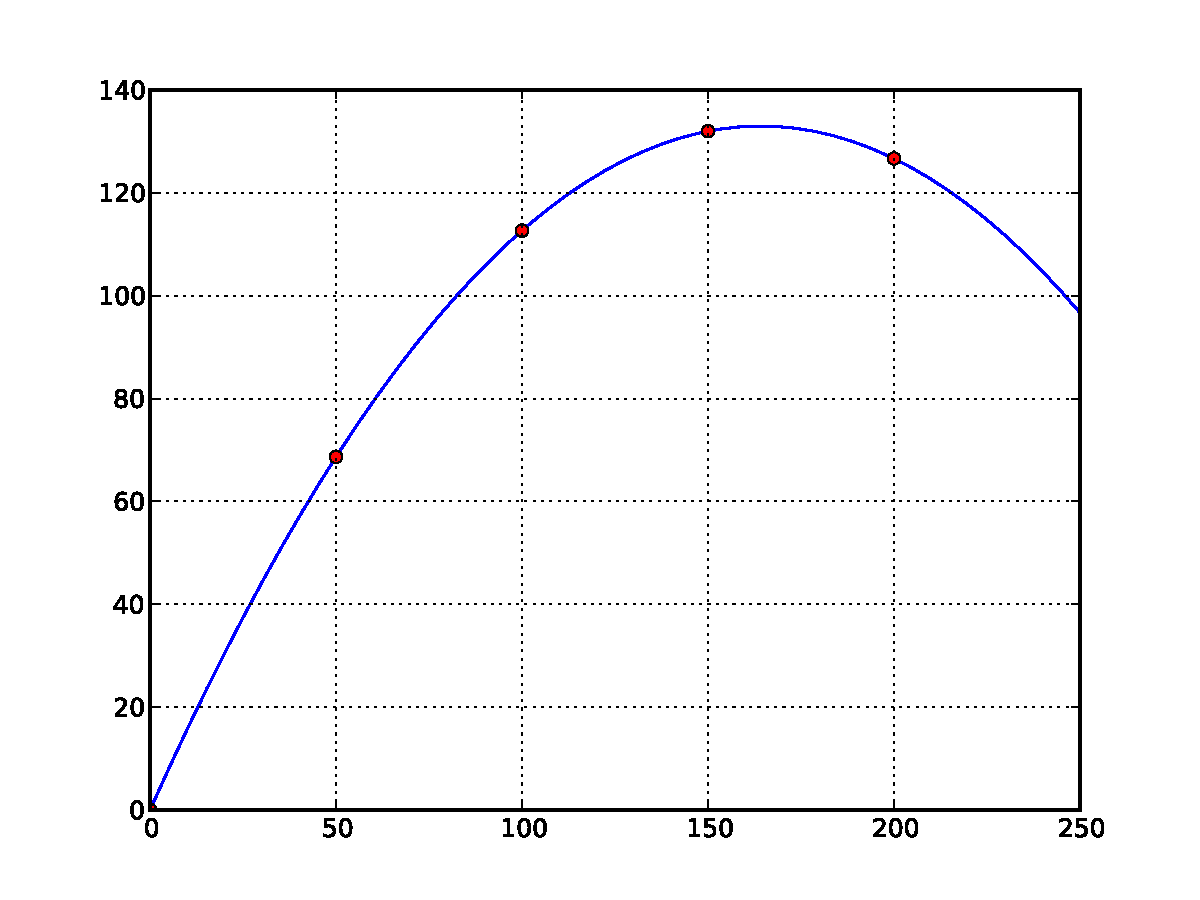
\includegraphics[scale=0.5]{trayectoria1}}%
%\only<2>{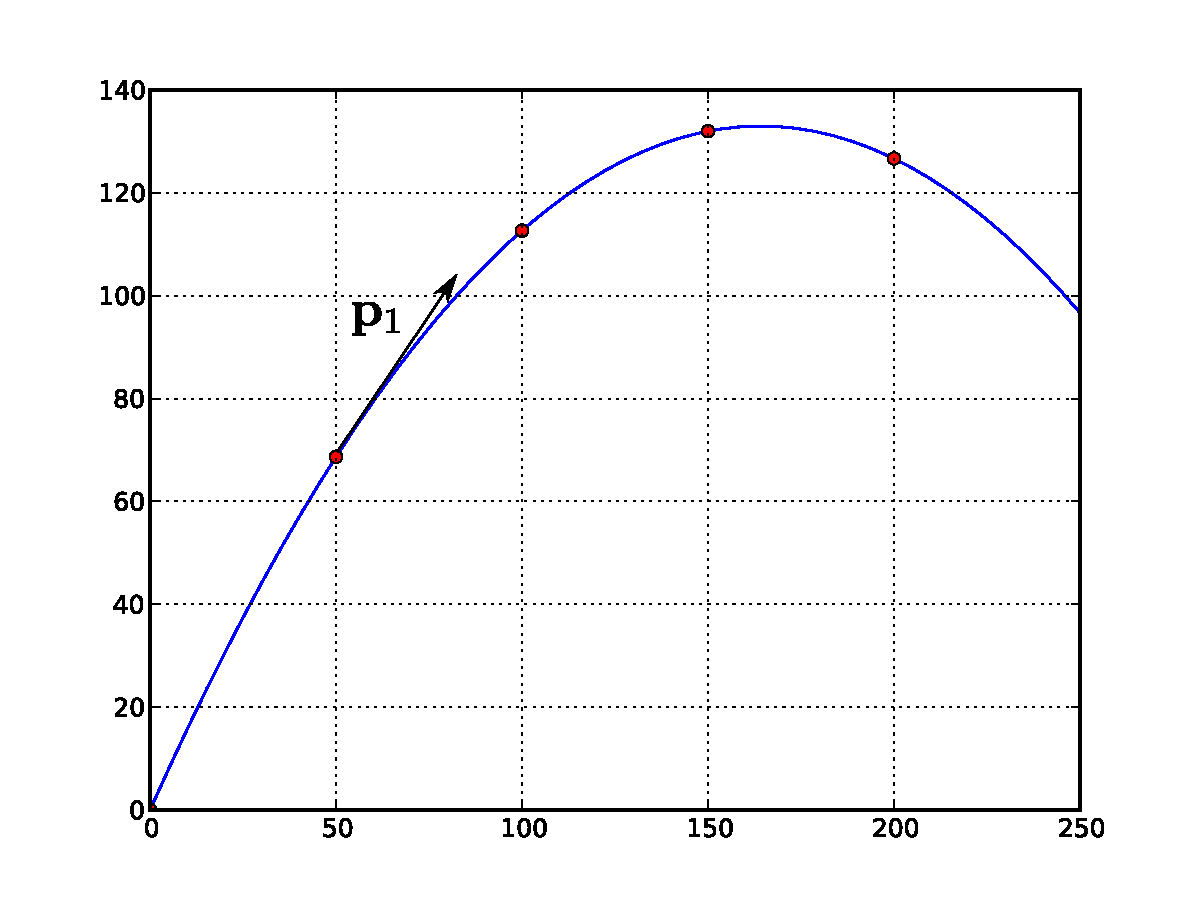
\includegraphics[scale=0.5]{trayectoria2}}%
%\only<3>{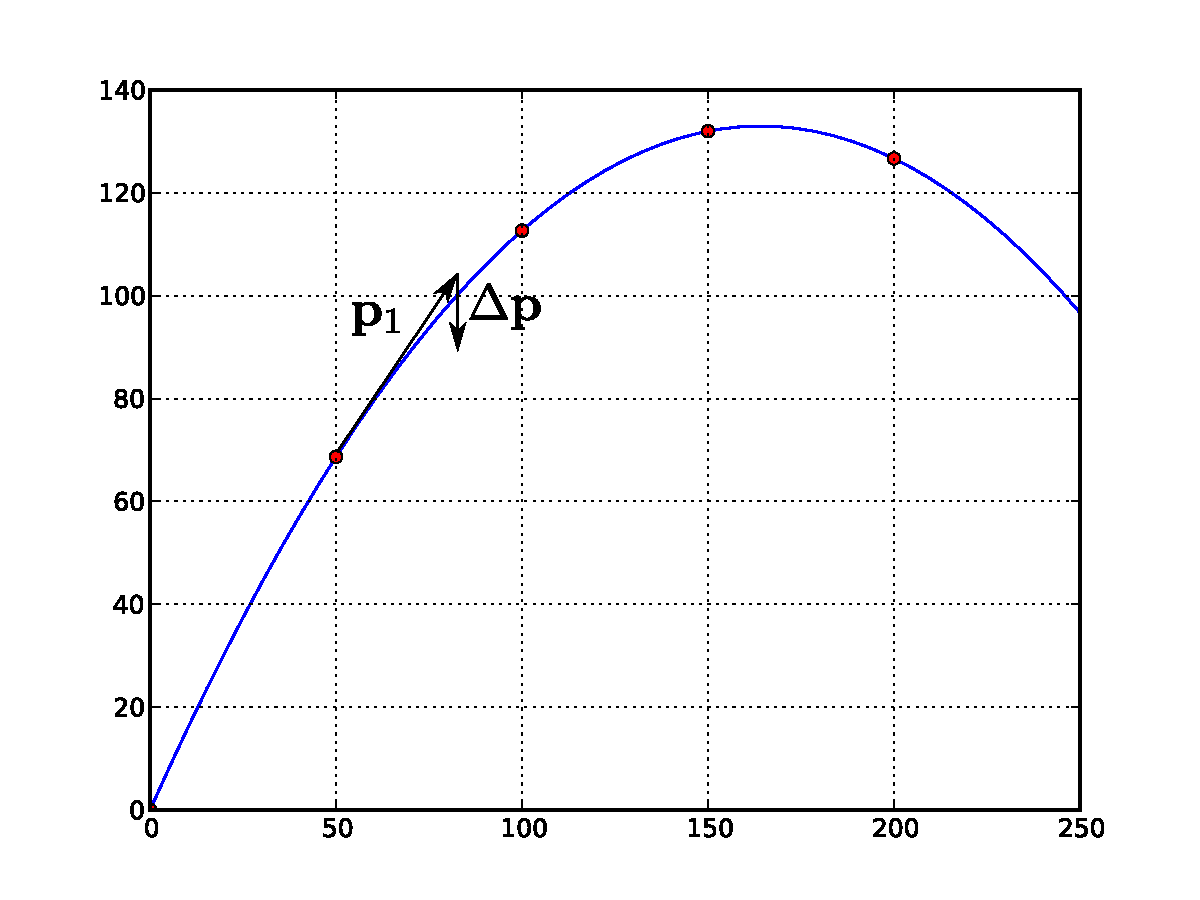
\includegraphics[scale=0.5]{trayectoria3}}%
%\only<4>{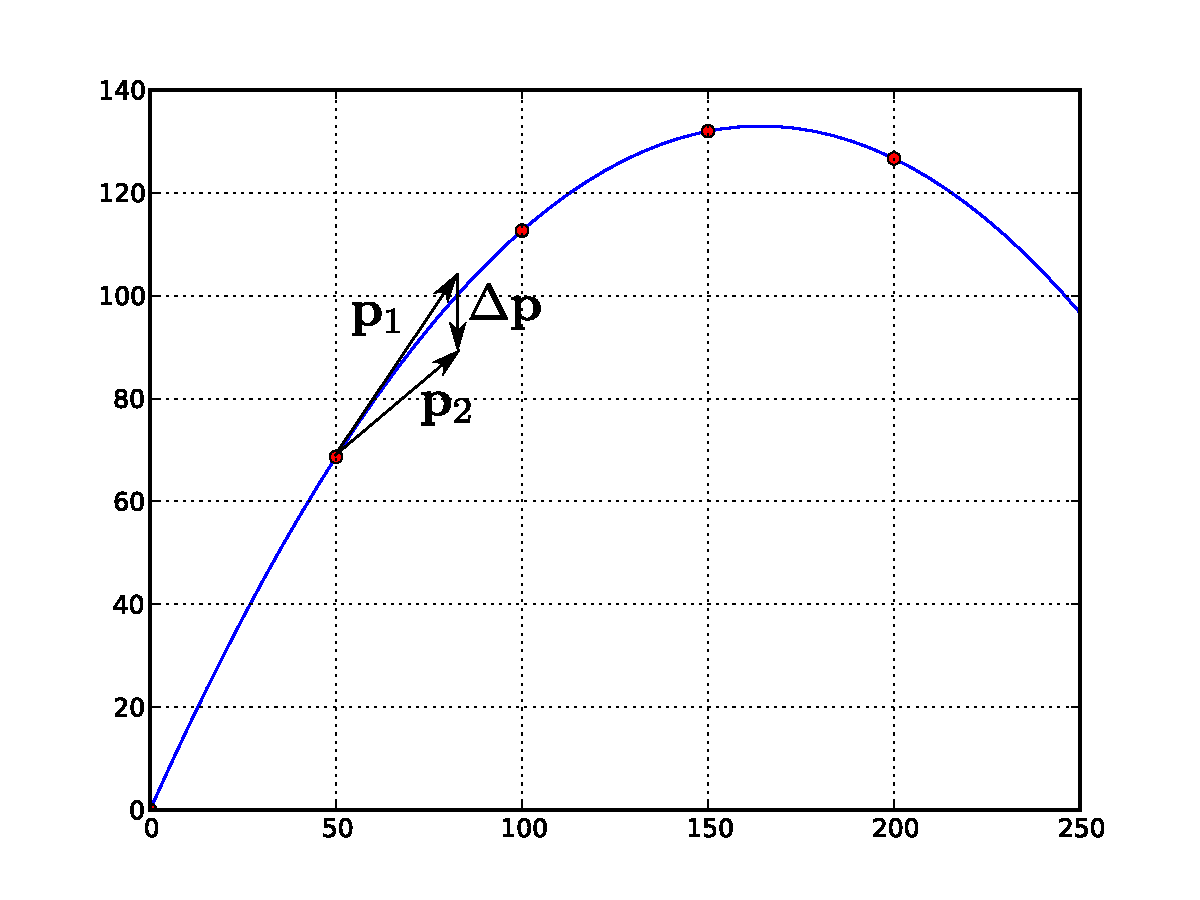
\includegraphics[scale=0.5]{trayectoria4}}%
%\only<5>%
{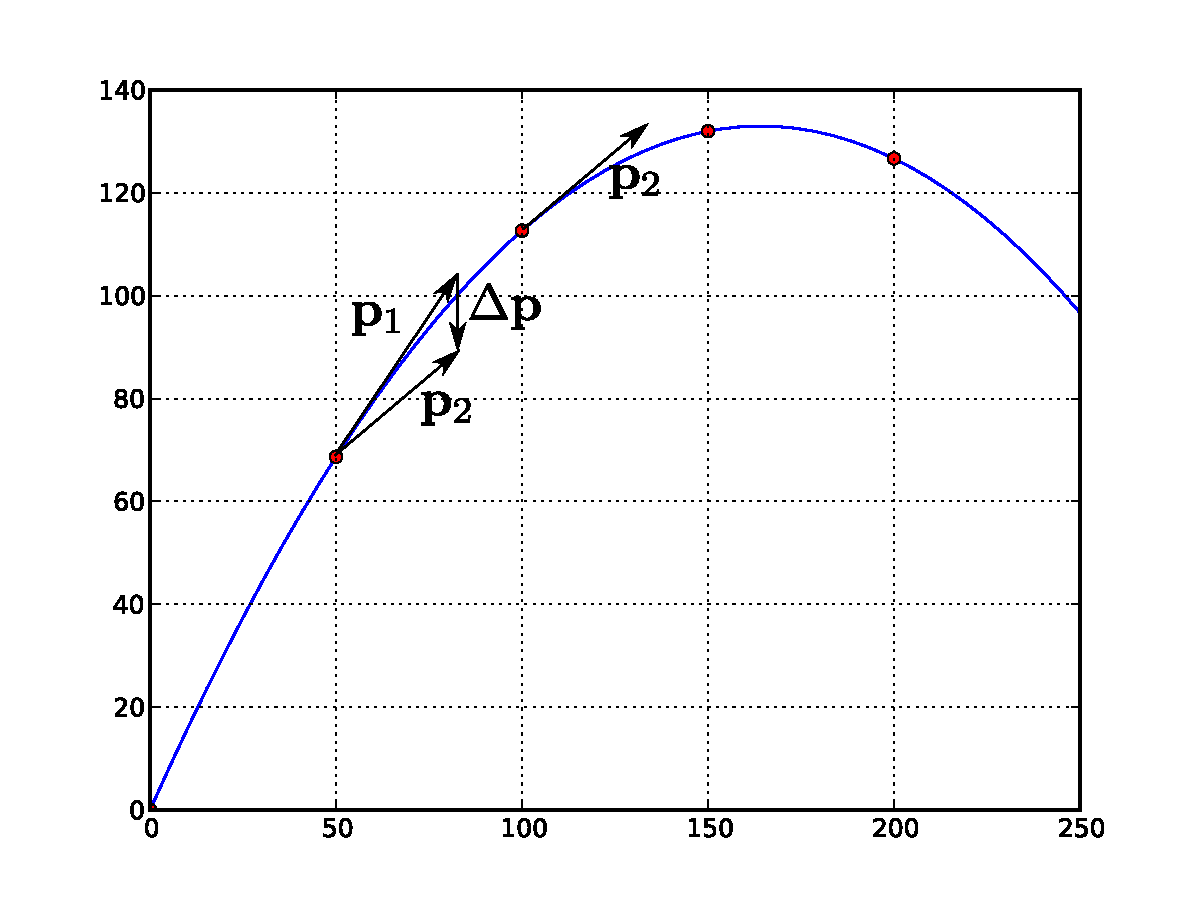
\includegraphics[scale=0.5]{trayectoria5}}
    \caption{Actualización del momentun}
    \label{fig:predtray}
  \end{figure}
\end{frame}

El proceso iterativo que se puede implementar computacionalmente equivale a hacer la integral sobre la ecuación de movimiento dada por el Principio de moméntum. Sin embargo, sólo en casos muy específicos se puede realizar analíticamente la integración de la ecuación de movimiento.

Para ilustrar la integración numérica considere el siguiente programa en \texttt{vpython} de la solución al problema de una partícula de masa $m=0.5\ $Kg, con velocidad inicial $\mathbf{v}_i=(5,0,0)\ $m/s, moviendose bajo la influencia de una fuerza neta gravitacional dada por
\begin{align}
\textbf{F}_{\text{neta}}=&(0,-mg,0)\nonumber\\
=&(0,-4.9,0)\si{\newton}\,,
\end{align}
La implementación con un paso de integración dado por un $\Delta t=\SI{0.01}{\second}$ se ilustra en el siguiente programa:

\begin{frame}[fragile,allowframebreaks]
\begin{lstlisting}
from visual import *
ball=sphere(make_trail=True,pos=vector(-5,5,0),radius=.3, color=color.magenta)
trail=curve(color=(1,1,1))
m=.5
g=9.8
v=vector(5,0,0)
p=m*v
deltat=0.01
Fg=vector(0,-m*g,0)
while True:
    #slow program
    rate(20)
    p=p+Fg*deltat
    ball.pos=ball.pos+(p/m)*deltat
    trail.append(pos=ball.pos)
    if ball.pos[0]>2: raw_input('Stop?')
\end{lstlisting}
\end{frame}

El resultado del programa es la simulación del evento paso a paso hasta alcanzar la posición mostrada en la figura~\ref{fig:CaidaLibreSimple}

\begin{frame}[plain]
  \begin{figure}
    \centering
    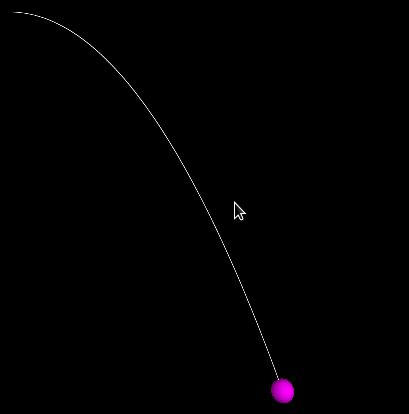
\includegraphics[scale=0.4]{CaidaLibreSimple}
    \caption{Movimiento parabólico integrado numéricamente}
    \label{fig:CaidaLibreSimple}
  \end{figure}
\end{frame}
Tomando el origen de coordenadas en el punto inicial de la bola, podemos obtener las primeras posiciones de la bola repitiendo el proceso manualmente. El resultado de las primeras cinco interacciones se muestra en la Tabla~\ref{tab:caidalibre}
\begin{table}
  \centering
  \begin{tabular}{|c|c|c|}\hline
    $t$ (\si{\second}) & $\mathbf{p}$ (\si{\kilo\gram \meter\per\second}) & $\mathbf{r}$ (\si{\meter})\\\hline
    0.01 & (2.5, -0.049, 0) & (0.05,-0.00098, 0)\\
    0.02 & (2.5, -0.098, 0) & (0.1, -0.00294, 0)\\
    0.03 & (2.5, -0.147, 0) & (0.15,-0.00588, 0)\\
    0.04 & (2.5, -0.196, 0) & (0.2, -0.0098,  0)\\
    0.05 & (2.5, -0.245, 0) & (0.25,-0.0147,  0)\\ 
    $\cdots$ & $\cdots$ & $\cdots$ \\ \hline
  \end{tabular}
  \caption{Primeras cinco posiciones de la bola con respecto al punto inicial}
  \label{tab:caidalibre}
\end{table}



Podemos complicar el programa poniendo rebotes sobre el piso. El programa modificado es
\begin{frame}[fragile,allowframebreaks]
\begin{lstlisting}
from visual import *
ball=sphere(make_trail=True,pos=vector(-5,5,0),radius=.3, color=color.magenta)
floor=box(pos=vector(0,-5,0), size=(12,0.1,12) , color=color.green)
trail=curve(color=(1,1,1))
m=.5
g=9.8
v=vector(0.5,0,0)
p=m*v
deltat=0.01
Fg=vector(0,-m*g,0)
while True:
    #slow programa
    rate(100)
    p=p+Fg*deltat
    ball.pos=ball.pos+(p/m)*deltat
    trail.append(pos=ball.pos)
    if ball.pos.y < floor.pos.y:
        p.y=-p.y

\end{lstlisting}
\end{frame}

\begin{frame}
  El programa genera una animación, de la cual  se ilustra uno de los cuadros en la figura~\ref{fig:caidalibre}
  \begin{figure}
    \centering
    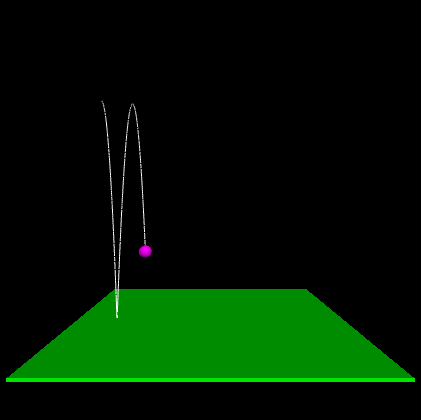
\includegraphics[scale=0.5]{caidalibre}
    \caption{Movimiento parábolico con rebote}
    \label{fig:caidalibre}
  \end{figure}

\end{frame}


Medir la velocidad de un objeto es una tarea familiar, pero ¿cómo
medimos la magnitud de una fuerza?

Una forma simple de medir una fuerza es usar el estiramiento o
compresión de un resorte. 
%Hacer diagrama.
Cuando colgamos un bloque de un resorte, notamos que el resorte se
estira una distancia $s$.  
Si doblamos el peso notamos que el resorte se estira el doble. 
De la misma manera un resorte en posición vertical es comprimido una
distancia $s$ por el mismo bloque, y el doble de la distancia con dos
bloques.

Por consiguiente, podemos usar un resorte para hacer una escala para
medir fuerzas, calibrándolo en términos de cuanta fuerza se necesita
para producir un determinando estiramiento.
 
\subsection{Fuerza de un resorte}

Una ley de fuerza describe matemáticamente como una fuerza depende en una situación. Para un resorte, se ha determinado experimentalmente que la fuerza ejercida por un resorte sobre un objeto pegado al resorte está dada por la siguiente ecuación:
\begin{align}
  \left| \mathbf{F}_{\text{resorte}} \right|=k|\Delta \mathbf{r}|
\end{align}
donde $|\Delta \mathbf{r}|$ es la magnitud del vector desplazamiento entre la posición inicial y final del objeto pegado al resorte, y $k$ es la \emph{constante elástica} del resorte. 

La constante elástica $k$ es un número positivo, y es una propiedad del resorte en particular. Entre más grande $k$ más fuerza se necesita para estirar el resorte. 

Para un resorte moviéndose en una dimensión y con el origen de coordenadas coincidiendo con la posición del objeto cuando el resorte esta relajado, tenemos que la fuerza que el resorte ejerce sobre el objeto cuando se estira una distancia $x$ es
\begin{align}
  \mathbf{F}=-k(x,0,0)
\end{align}


Si consideremos un resorte con un cuerpo pegado a su extremo moviéndose sobre una superficie, debemos considerar la fuerza de fricción entre el cuerpo y la superficie. La Ley que describe esta fuerza fricción $f$, encontrada también por experimentación, es
\begin{align}
  |\mathbf{f}|=\mu m g\,,
\end{align}
donde $\mu$ es el \emph{coeficiente de fricción entre el cuerpo y la superficie}, $m$ es la masa del cuerpo y $g$ es la aceleración gravitacional cerca a la superficie de la Tierra. La dirección de la fuerza de fricción es siempre opuesta a la dirección de movimiento. 

Con está información y con el principio de moméntum podemos simular el movimiento de un cuerpo unido a un resorte sobre una superficie horizontal. La explicación paso a paso del funcionamiento del programa puede encontrarse en este \href{http://nbviewer.ipython.org/urls/raw.github.com/rescolo/spring/master/spring.ipynb}{link}. Mientras el programa definitivo es

\begin{frame}[fragile,allowframebreaks]
\begin{lstlisting}
from __future__ import division
from visual import *


# INITIALIZE WINDOW AND DECLARATIONS

scene.range = vector(1,1,1)
scene.center = vector(0,0,0)
scene.width = 800
scene.height = 600

# CREATE SPRING, WEIGHT AND LABEL OBJECTS

relaxedlength = vector(.60,0,0) # length of spring when it isn't stretched or compressed
spring = helix(pos=(-.75,0,0),axis=relaxedlength, radius=.1,coils=8,thickness=.01,color=color.green)

weight = box(pos=(0,0,0),size=(.3,.3,.3),color=color.yellow)

frictionlessSurface = box(size=(2,.02,.5),pos=(0,-.16,0))
wall = box(size=(.04,.5,.3),pos=(-.77,.1,0),color=color.red)


# SET INITIAL CONDITIONS

spring.constant = 2 # k
weight.mass = 10 # kg
weight.velocity = vector(0,0,0)
weight.acceleration = vector(0,0,0)
weight.force = vector(0,0,0)

#Set the label position
mylabel = label(pos=(0,.4,0))
#spring.displacement
xpos=0.35 
weight.pos=vector(xpos,0,0)
spring.displacement=weight.pos
spring.axis=relaxedlength+spring.displacement
# message to the user
message = "Inititial position:"
message += "\ndisplacement: %.2f" % spring.displacement.x 
mylabel.text = message

\end{lstlisting}
\end{frame}

\subsection{Integración analítica}
Al proceso de evolucionar un sistema a través del tiempo se le llama
integración del movimiento. En algunos caso especiales dicha
integración se puede realizar de forma analítica. El proceso
matemático de integrar una función $f(x)$ en el intervalo $a$, $b$, corresponde a evaluar el área bajo la curva en ese intervalo
\begin{align}
  \int_a^b f(x)\,dx\approx&f(x_0)(x_1-x_0)+f(x_1)(x_2-x_1)+\cdots+f(x_{n-1})(x_n-x_{n-1}) \nonumber\\
\lim_{\Delta x\to 0}\sum_{i=0}^n\,f(x_i)\Delta x_i\,,
\end{align}
donde $f(x_0)=1$, $f(x_{n})=b$ y $\Delta x_i=x_{i+1}-x_i$.

Se puede demostrar que
\begin{align}
  \int_a^b f(x)\,dx=\left. F(x)  \right|_a^b
\end{align}


\begin{table}
  \centering
  \begin{tabular}{lll}
    $f(x)$ & derivada & integral\\
  \end{tabular}
  \caption{Tabla de integrales}
\end{table}

De este modo, por ejemplo, la integral de la función $f(x)=x$ entre $0$ y $a$ es
\begin{align}
  \int_0^a x\,dx=\left.\frac{1}{2}x^2\right|_0^a=\frac{1}{2}a^2\,,
\end{align}
y el área del triángulo correspondiente es
\begin{align}
  \frac{1}{2}\text{base}\times\text{altura}=\frac{1}{2}a^2\,,
\end{align}

Así mismo la integral de una rapidez constante $v$, entre $t_1$ y $t_2$ para un movimiento en línea recta
\begin{align}
  \int_{t_1}^{t_2}v \,dt=v(t_2-t_1)=d=\text{distancia recorrida entre $t_1$ y $t_2$.}
\end{align}
En general, el área de la curva en línea recta de la velocidad en
función del tiempo corresponde a la distancia recorrida. Para el
gráfico de distancia en función del tiempo de la
Fig.~\ref{fig:vinstaprom3}, tendríamos en el plano velocidad en
función del tiempo, una línea recta horizontal entre cero y
$\SI{1}{h}$, una línea recta de $\SI{70}{km/h}$, con área bajo la
curva $\SI{70}{km}$, y otra línea recta entre $\SI{1}{h}$ y
$\SI{2}{h}$ con área $\SI{30}{km}$ para una distancia total recorrida
de $\SI{100}{km}$.

\subsection{Ecuación de movimiento}


Como para un $\Delta t$ infinitesimal, la fuerza siempre se puede considerar constante, el principio de momentum se puede reescribir como
\begin{align}
  \label{eq:28}
  \mathbf{F}_{\text{neta}}=&\lim_{\Delta t\to 0}\frac{\Delta\mathbf{p}}{\Delta t}\nonumber\\
 \mathbf{F}_{\text{neta}}=&\frac{d\mathbf{p} }{dt}
\end{align}
Si $\mathbf{F}_{\text{neta}}$ es conocida, a la ec.~\eqref{eq:28}, se conoce como ecuación de movimiento.

\begin{frame}
  \begin{block}%
{Ecuación de movimiento:}
  \begin{align*}
   \mathbf{F}_{\text{neta}}=&\frac{d\mathbf{p} }{dt}
   \end{align*}
  \end{block}
\end{frame}



\subsection{Caso especial: masa constante}
En el caso especial en que la masa del sistema, $m$, es constante, la ecuación de movimiento puede reescribirse como
\begin{align}
   \mathbf{F}_{\text{neta}}=&\frac{d m\mathbf{v} }{dt}\nonumber\\
   \mathbf{F}_{\text{neta}}=&m\frac{d \mathbf{v} }{dt}\nonumber\\
   \mathbf{F}_{\text{neta}}=&m\mathbf{a}\,.
\end{align}

\begin{frame}
  \begin{block}%
{Caso especial: masa constante}
\begin{align}
   \mathbf{F}_{\text{neta}}=&m\mathbf{a}\,.
\end{align}
\end{block}
\end{frame}

\subsection{Caso especial: Fuerza y masa constante}

Si la fuerza neta es constante en dirección y magnitud en el caso de masa constante, la ecuación de movimiento puede integrarse analíticamente. Para simplificar el análisis consideremos una fuerza neta constante sólo con componente en $x$:
\begin{align}
  \mathbf{F}_{neta}=(F_x,0,0)\,.
\end{align}

La ecuación de movimiento se reduce a
\begin{align}
  a_x=&\frac{F_x}{m}\nonumber\\
\frac{dv_x}{dt}=&\frac{F_x}{m}\nonumber\\
{dv_x}=&\frac{F_x}{m}{dt}\,.
\end{align}
Integrando a ambos lados de la igualdad, desde un tiempo inicial $t_i$ a un tiempo final $t$, con $v_{xi}=v_x(t_i)$ y $v_x=v_x(t)$, tenemos
\begin{align}
  \int_{v_{xi}}^{v_x} d v_x =&\int_{t_i}^t \frac{F_x}{m}{dt}\nonumber\\
  v_x-v_{xi} =&\frac{F_x}{m}\int_{t_i}^t {dt}\,
\end{align}
y despejando en términos de la velocidad final
\begin{align}
  \label{eq:36}
  v_x =&v_{xi}+\frac{F_x}{m}(t-t_i)\nonumber\\
=&v_{xi}+\frac{F_x}{m}\Delta t\,.
\end{align}
Integrando de nuevo
\begin{align}
  \frac{dx}{dt} =&v_{xi}+\frac{F_x}{m}(t-t_i)\nonumber\\
  {dx} =&v_{xi}{dt}+\frac{F_x}{m}(t-t_i){dt}\,,
\end{align}
e integrando de nuevo con $x_i=x(t_i)$ y $x=x(t)$, tenemos
\begin{align}
  \int_{x_i}^{x}{dx} =&v_{xi}\int_{t_i}^t{dt}+\frac{F_x}{m}\int_{t_i}^t{dt}(t-t_i){dt}\,.
\end{align}
Haciendo $u=t-t_i$, $du=dt$, obtenemos
\begin{align}
\int(t-t_i)dt=\int u du=\frac{1}{2}u^2=\frac{1}{2}(t-t_i)^2\,,
\end{align}
de modo que
\begin{align}
  x-x_i=&v_{xi}(t-t_i)+\frac{F_x}{m}\left.\frac{1}{2}(t-t_i)^2\right|^t_{t_i}
\end{align}
\begin{align}
  x=&x_i+v_{xi}(t-t_i)+\frac{1}{2}\frac{F_x}{m}
  \left[
    (t-t_i)^2-(t_i-t_i)^2
  \right]\nonumber\\
  x=&x_i+v_{xi}(t-t_i)+\frac{1}{2}\frac{F_x}{m}(t-t_i)^2
\end{align}
\begin{frame}
  \begin{block}%
{Solución analítica:} al problema de movimiento en una dimensión bajo la influencia de una fuerza constante
\begin{align}
   x=&x_i+v_{xi}(t-t_i)+\frac{1}{2}\frac{F_x}{m}(t-t_i)^2\nonumber\\
   =&x_i+v_{xi}\Delta t+\frac{1}{2}\frac{F_x}{m}\Delta t^2\,.
\end{align}
  \end{block}
\end{frame}

Si eliminamos $\Delta t$, usando la ec.\eqref{eq:36}, tenemos
\begin{align*}
  x=&x_i +v_{xi}(v_x-v_{xi})\frac{m}{F_x}+\frac{1}{2}\frac{F_x}{m}(v_x-v_{xi})^2\frac{m^2}{F_x^2}\nonumber\\
  x=&x_i +(v_{xi}v_x-v_{xi}^2)\frac{m}{F_x}+\frac{1}{2}(v_x^2-2 v_x v_{xi}+v_{ix}^2)\frac{m}{F_x}\nonumber\\
x=&x_i +\frac{1}{2}(v_x^2-v_{ix}^2)\frac{m}{F_x}\,.
\end{align*}
Reorganizando términos tenemos
\begin{align}
  \label{eq:tray0}
  v_x^2-v_{ix}^2=-2\frac{F_x}{m}(x-x_i)\,.
\end{align}


Un ejemplo de fuerza constante, es la fuerza gravitacional sobre un objeto de masa $m$ que se encuentra cerca a la superficie de la tierra:
\begin{align}
  \label{eq:29}
  \mathbf{F}_{\text{grav}}=(0,F_y,0)\approx(0,-mg,0).
\end{align}
El signo menos índica que la fuerza va dirigida hacía la superficie de la tierra, donde hemos establecido el origen de coordenadas

Si dicho cuerpo cae libremente desde una altura $y_i$ desde la superificie de la tierra, y con una velocidad $v_{yi}$, la ecuación para su altura $y$ desde un origen de coordenadas sobre la superficie de la tierra es
\begin{align}
\label{eq:31}
   y=&y_i+v_{yi}(t-t_i)+\frac{1}{2}\frac{F_y}{m}(t-t_i)^2\nonumber\\
   y=&y_i+v_{yi}(t-t_i)-\frac{1}{2}g(t-t_i)^2\,.
\end{align}
mientras que para la componente de la velocidad en $y$, tenemos de la ec.~\eqref{eq:36}
\begin{align}
  \label{eq:37}
    v_y =&v_{yi}-g(t-t_i)\,,
\end{align}

\begin{frame}
  \begin{block}%
{Solución analítica:} al problema de caida libre en la dirección $y$ perpendicular a la superficie de la tierra y con origen de coordenadas sobre la superficie de la tierra:
\begin{align*}
     y=&y_i+v_{yi}(t-t_i)-\frac{1}{2}g(t-t_i)^2\nonumber\\
     v_y =&v_{yi}-g(t-t_i)\nonumber\\
     a_y=&-g\,.
\end{align*}

  \end{block}
\end{frame}


\subsection{Ecuación de la trayectoria}
Para un cuerpo en movimiento vertical bajo la influencia de una fuerza gravitacional constante, tenemos que si la rapidez inicial es $v_0$ para una altura inicial $y_0$, entoces de \eqref{eq:37}
\begin{align}
  \Delta t=\frac{v_0-v}{g}
\end{align}
sustituyendo en ec.~\eqref{eq:caidalibre}
\begin{align}
  y-y_0=&v_0(v_0-v)/g-\tfrac{1}{2}g(v_0-v)^2/g^2\nonumber\\
       =&v_0^2/g-vv_0/g-\tfrac{1}{2}(v_0^2/g-2vv_0/g+v^2/g)\nonumber\\
       =&\tfrac{1}{2}v_0^2/g-\tfrac{1}{2}v_0^2/g\nonumber\\
       =&\tfrac{1}{2}(v_0^2-v^2)/g\,,
\end{align}
de donde obtenemos la ecuación de la trayectoria (vec eq.~(\ref{eq:tray0}):
\begin{align}
  \label{eq:trayectoriay}
  v^2-v_0^2=-2g(y-y_0)\,,
\end{align}
Esta \'ultima ecuaci\'on esta relacionada con la conservaci\'on de energ\'\i a cin\'etica m\'as energ\'\i a potencia, como se definir\'a luego.


\subsection{Conservación de momentum}
Volviendo al problema general, de la ec.~\eqref{eq:28} podemos ver que si el momentum es constante (en dirección, magnitud y masa)
\begin{align}
  \mathbf{F}_{\text{neta}}=&\frac{d\mathbf{p}}{dt}\nonumber\\
=&0\,.
\end{align}
En otras palabras:
\begin{frame}
  \begin{block}%
{Ley de Conservación de Moméntum:} \textbf{Si la fuerza neta actuando sobre un sistema es cero, el momentum total del sistema es constante}
  \end{block}
\end{frame}

En componentes:
\begin{align}
  F_{\text{neta},x}=&\frac{d p_x}{dt}\nonumber\\
  F_{\text{neta},y}=&\frac{d p_y}{dt}\nonumber\\
  F_{\text{neta},z}=&\frac{d p_z}{dt}\,,
\end{align}
y podemos ver que si alguna dirección del moméntum es constante, entonces la fuerza neta en esa dirección es cero, y viceverza. 

De acuerdo al teorema de Noether debe existir una simetría asociada a
la conservación de cada una de la direcciones del moméntum. 
La simetría correspondiente es la homogeneidad del espacio en cada una
de sus tres direcciones independientes.
Esta simetría se refleja en el hecho de que si realizamos un
experimento en un sitio determinado y luego lo repetimos en el
laboratorio de al lado, del frente, o del piso superior, debemos
obtener exactamente el mismo resultado. 
La regla de transformación correspondiente es que las leyes de la física deben ser invariante bajo el cambio, por ejemplo
\begin{align*}
  x\to x'=x+a\,,
\end{align*}
con $a$ constante.
En efecto
\begin{align*}
  F'_{\text{neta},x}=&\frac{dp'_{x}}{dt}\nonumber\\
=&m\frac{dv'_{x}}{dt}\nonumber\\
=&m\frac{d}{dt}\frac{dx'}{dt}\nonumber\\
=&m\frac{d}{dt}\frac{d(x+a)}{dt}\nonumber\\
=&m\frac{d}{dt}\frac{d(x)}{dt}\nonumber\\
=&m\frac{dv_{x}}{dt}\nonumber\\
=&\frac{dp_{x}}{dt}=F_{\text{neta},x}\,,
\end{align*}
de modo que dos observadores en dos laboratorios separados por una
distancia $x'=x+a$, deben medir la misma cantidad de movimiento para
el movimiento de un cuerpo sometido a una fuerza $F_{\text{neta},x}$.



En el caso de la fuerza gravitacional, si despreciamos la resistencia del aire, de la ec.~\eqref{eq:29} podemos ver que que la fuerza neta en $x$ y en $z$ es cero. Por lo tanto el momentum inicial en la dirección $x$ y $z$ se debe conservar. 

Supongamos que un cuerpo se mueve bajo la influencia de la fuerza gravitacional en un planeta sin atmosfera con aceleración gravitacional $g$. Por simplicidad, escojamos como $x$ la dirección inicial del cuerpo paralela a la superficie del planeta. Dicha dirección se debe mantener constante, de modo que
\begin{align*}
  \frac{d p_x}{dt}=&0\nonumber\\
  m\frac{d v_x}{dt}=&0\nonumber\\
  \frac{d v_x}{dt}=&0\nonumber\\
  {d v_x}=&0\nonumber\\
  \int_{v_{xi}}^{v_x}{d v_x}=&0\nonumber\\
  v_x-v_{xi}&=0\nonumber\\
  v_x=&v_{xi}\,.
\end{align*}
integrando de nuevo
\begin{align}
  \frac{dx}{dt}=&v_{xi}\nonumber\\
  dx=&v_{xi}{dt}\nonumber\\
  \int_{x_i}^x dx=&v_{xi}\int_{t_i}^t{dt}\nonumber\\
  x-x_i=&v_{xi}(t-t_i)\,.
\end{align}
y recuperamos la
\begin{frame}
  \begin{block}%
{solución analítica:} al problema del movimiento en una dimensión en ausencia de fuerzas externas
\begin{align}
  \label{eq:30}
  x=&x_i+v_{xi}(t-t_i)\,.
\end{align}
  \end{block}
\end{frame}

Combinado las ecuaciones \eqref{eq:30} y \eqref{eq:31} obtenemos la
\begin{frame}
  \begin{block}%
{solución analítica:} al problema de movimiento parábolico despreciando la resistencia del aire
\begin{align}
  \label{eq:32}
  x=&x_i+v_{xi}(t-t_i)=x_i+v_{xi}\Delta t\nonumber\\
  y=&y_i+v_{yi}(t-t_i)-\frac{1}{2}g(t-t_i)^2=y_i+v_{yi}\Delta t-\frac{1}{2}g\Delta t^2\,.
\end{align}
El vector de desplazamiento es
\begin{align}
\mathbf{r}=(x,y,0)
\end{align}
%hacer diagrama
Derivando con respecto al tiempo obtenemos las velocidades (ver ec.~\eqref{eq:37})
\begin{align}
  \label{eq:33}
  v_x=\frac{dx}{dt}=&v_{xi}&\text{velocidad constante}\nonumber\\
  v_y=\frac{dy}{dt}=&v_{yi}-\frac{1}{2}g(2(t-t_i))&\nonumber\\
  =&v_{yi}-g(t-t_i)&\text{aceleración constante}\,,
\end{align}

  \end{block}
\end{frame}



\begin{itemize}
\item[\textbf{Ejemplo:}] \textbf{Una bola con resistencia de aire despreciable (2D, Fuerza constante):}
Una bola de masa 500~g está inicialmente en el suelo, en una ubicación $(0,0,0)\ $m. La bola es entonces pateada con una velocidad inicial $(3,7,0)\ $m/s.
\begin{enumerate}
\item ¿Donde estará la bola medio segundo después?
\label{item:8}
\item ¿En que tiempo la bola golpeará el piso?
\label{item:9}
\end{enumerate}
Haga la aproximación que la resistencia del aire es despreciable.


\item[\textbf{Solución:}] Sistema: bola\\
Entorno: Tierra\\
Diagrama de cuerpo libre: ver figura\\
Tiempo inicial: El instante en que el pie ya no esta en contacto con la bola
\begin{itemize}
\item[~\ref{item:8}]
Después de medio segundo, y como se ilustra en la figura~\ref{fig:parabgraph1}
\begin{align}
  x_f=&x_i+v_{xi}\Delta t\nonumber\\
  =&0+(3\ \text{m/s})(0.5\ \text{s})=1.5\ \text{m}
\end{align}
Para el movimiento en $y$ tenemos
\begin{align}
  y_f=&y_i+v_{yi}\Delta t-\frac{1}{2}g \Delta t^2\nonumber\\
=& 0+(7\ \text{m/s})(0.5\ \text{s})-\frac{1}{2}(9.8\ \text{N/kg})(0.5\ \text{s})^2=2.275\ \text{m}
\end{align}
El vector final de desplazamiento después de $\SI{0.5}{\second}$ es
\begin{align}
  \mathbf{r}_f=(1.5,2.75,0)\ \text{m}
\end{align}
Comprobación: Las unidades son correctas, y la bola se ha movido en la dirección apropiada
\item[~\ref{item:9}] Tiempo final: El instante justo antes de que la bola golpee el piso. En ese instante sabemos que $y_f=0$, de modo que podemos encontrar $\Delta t$
  \begin{align*}
    0=0+v_{yi}\Delta t-\frac{1}{2}g\Delta t^2
  \end{align*}
  \begin{align*}
 \Delta t(v_{yi}-\frac{1}{2}g\Delta t)=0   
  \end{align*}
con soluciones
  \begin{align}
    \Delta t=&0 &\text{o}\qquad v_{yi}-\frac{1}{2}g\Delta t=&0
  \end{align}
El segundo valor es el tiempo cuando la bola retorna al suelo
\begin{align}
  \Delta t=&\frac{2 v_{yi}}{g}\nonumber\\
=&\frac{2(\SI{7}{m/s})}{\SI{9.8}{\newton\per\kilo\gram}} =\SI{1.43}\ \text{s}
\end{align}
El movimiento en $y$ es ilustrado en la figura~\ref{fig:parabgraph3}, mientras que la trayectoria real es ilustrada en la figura~\ref{fig:parabgraph5}.
\end{itemize}

\end{itemize}



\begin{frame}
\begin{figure}
  \centering
  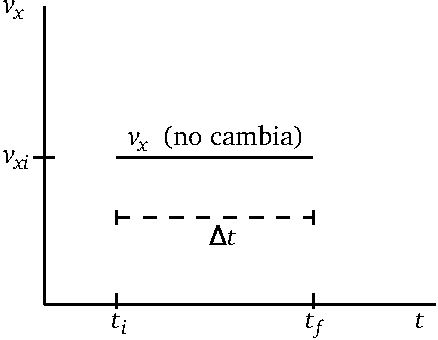
\includegraphics[scale=0.9]{parabgraph1} 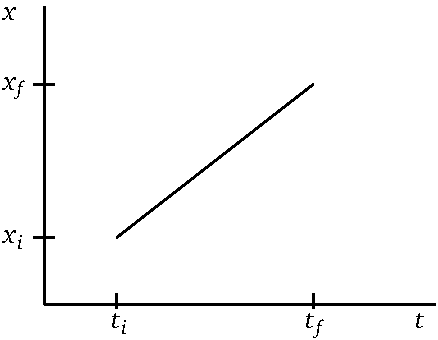
\includegraphics[scale=0.9]{parabgraph2}
  \caption{Movimiento de la bola en $x$}
  \label{fig:parabgraph1}
\end{figure}
\end{frame}

\begin{frame}
\begin{figure}
  \centering
  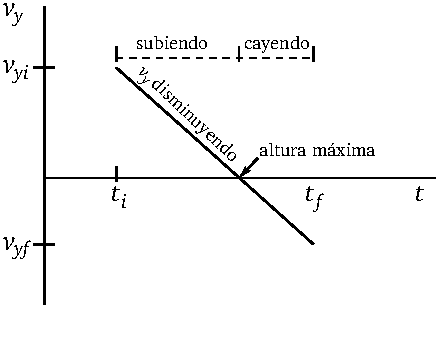
\includegraphics[scale=0.9]{parabgraph3}  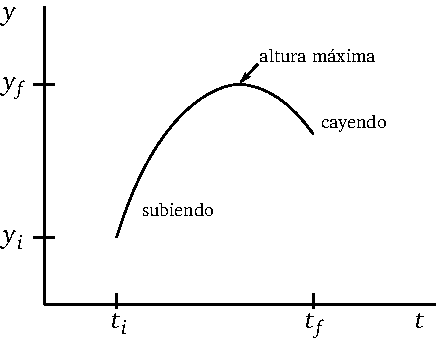
\includegraphics[scale=0.9]{parabgraph4}
  \caption{Movimiento de la bola en $y$}
  \label{fig:parabgraph3}
\end{figure}
\end{frame}

\begin{frame}
\begin{figure}
  \centering
  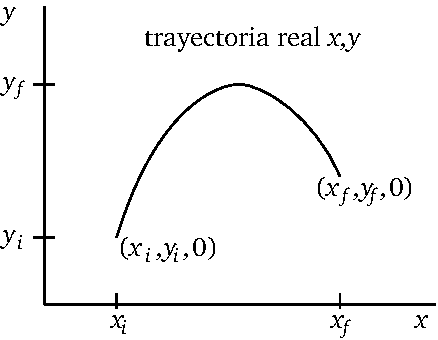
\includegraphics{parabgraph5}
  \caption{Movimiento de la bola en el plano $x-y$}
  \label{fig:parabgraph5}
\end{figure}
\end{frame}

\subsection{Ejemplos movimiento parabólico}

\begin{inprogress}
  Ejemplo notas Kowalski 3-13
\end{inprogress}

\begin{itemize}
\item[\textbf{Ejemplo:}] Una piedra es lanzada hacia arriba desde lo alto de un edificio con una velocidad inicial de 20 m/s directamente hacia arriba. El edificio tiene 50 m de alto, y la piedra falla en golpear el edificio en su camino hacia abajo.
  \begin{enumerate}
  \item \textquestiondown Qu\'e tiempo le toma a la piedra alcanzar su m\'axima altura?
    \begin{align}
      v(t)=v_0-gt\,.
    \end{align}
    A la altura m\'axima $v=0$, y con $v_0=+20$ m/s
    \begin{align}
      t_{\text{max}}=&\frac{v_0}{g}\nonumber\\
      =&\frac{20}{9.8}\ s\nonumber\\
      \approx&2.04\ s
    \end{align}
  \item \textquestiondown Cual es la m\'axima altura desde la base del edificio?:\\
    Tomando el origen de coordenadas en la base del edificio:
    \begin{align}
      y_{\text{max}}=&y_0+v_o t-\frac{1}{2}g t^2\nonumber\\
      \approx&50+20\timesm2.04-\tfrac{1}{2}\timesm9.8\timesm(2.04)^2\nonumber\\
      \approx&70.4\ \text{m}\,,
    \end{align}
  \item \textquestiondown Cual es el tiempo necesario para que la piedra retorne al nivel de la torre?\\
    \begin{align}
      t_{\text{torre}}=2t_{\text{max}}\approx4.08\ \text{s}\,.
    \end{align}
  \item \textquestiondown La velocidad a ese instante?\\
    \begin{align}
      v=&v_0-gt\nonumber\\
      \approx&20-9.8\timesm4.08\\
      v_{\text{torre}}\approx&-20\ \text{m/s}\,,
    \end{align}
    La misma magnitud que la velocidad inicial pero con direcci\'on opuesta. La velocidad incial estar\'\i a representada por un vector $\mathbf{v}_0$: $\uparrow$, mientras que $\mathbf{v}_{\text{torre}}:$ $\downarrow$.
  \item \textquestiondown Cual es la velocidad y posici\'on (desde la base del edificio) despu\'es de $t=5\ \text{s}$?
    \begin{align}
      v(5)\approx 20-9.8\timesm5\approx-29.0\ \text{s}\,.
    \end{align}
    \begin{align}
      y(5)\approx50+20\timesm5-\tfrac{1}{2}\timesm9.8\timesm5^2\approx27.5\ \text{m}\,.
    \end{align}
  \item \textquestiondown Cual es la velocidad y el tiempo cuando la piedra golpea el piso?
    \begin{align}
      y_0=&50\ \text{m} & y_{\text{final}}=0\nonumber\\
      \mathbf{v}_0=&20\hat{\mathbf{j}}\ \text{m/s} & \\
    \end{align}

    \begin{align}
      v^2=&v_0^2-2g(y_{\text{final}}-y_0)\nonumber\\
      =&v_0^2-2g(0-y_0)\nonumber\\
      \approx&20^2+2\timesm9.8\timesm 50\,,
    \end{align}
de donde
\begin{align}
  \mathbf{v}_{\text{final}}=-37.1 \hat{\mathbf{j}}\ \text{m/s}\,.
\end{align}
\begin{align}
  t_{\text{final}}=&(v_0-v_{\text{final}})/g\nonumber\\
  \approx&(20+37.1)/9.8\approx5.83\,s
\end{align}
  \end{enumerate}
\end{itemize}

\subsection{Movimiento parabólico completo}

En un movimiento parabólico completo, donde un cuerpo es lanzado desde
el suelo con cierta velocidad inicial y retorna al suelo sobre una
superficie horizontal, podemos especificar el alcance $R$ y la altura
máxima $y_{\text{max}}$ en términos de la rapidez inicial, $v$, y el
ángulo de lanzamiento $\theta$. Como
$\mathbf{r}_i=(x_i,y_i,0)=(0,0,0)$, tenemos
  \begin{enumerate}
  \item Altura máxima: se obtiene de la condición $v_y=0$. Reemplazando en la ec.~\eqref{eq:33}
    \begin{align}
      0=v_{yi}-g\Delta t\,,
    \end{align}
de modo que para alcanzar $y_{\text{max}}$ el cuerpo se tarda
\begin{align}
  \label{eq:34}
  \Delta t=\frac{v_{yi}}{g}\,.
\end{align}
Reemplazando \eqref{eq:34} en \eqref{eq:32}, tenemos
\begin{align}
  y_{\text{max}}=&v_{yi}\frac{v_{yi}}{g}-\frac{1}{2}g\frac{v_{yi}^2}{g^2}\nonumber\\
  =&\frac{v_{yi}^2}{g}-\frac{1}{2}\frac{v_{yi}^2}{g}\nonumber\\
  =&\frac{1}{2}\frac{v_{yi}^2}{g}\,.
\end{align}
En términos de la rapidez inicial y el ángulo de lanzamiento tenemos
\begin{align}
  y_{\text{max}}=\frac{v^2_i}{g}\sin^2\theta\,,
\end{align}
La mayor de las alturas máximas se obtiene para $\theta=\pi/2=90^\circ$, es decir cuando la velocidad inicial está toda en $y$.
\item Alcance: se obtiene de la condición: $y=0$. Reemplazando en la ec.~\eqref{eq:32}
  \begin{align}
    0=&v_{yi}\Delta t-\frac{1}{2}g\Delta t^2\nonumber\\
    =&\Delta t(v_{yi}-\frac{1}{2}g\Delta t)\to
    \begin{cases}
      \Delta t=0 & x=0\\
      v_{yi}-\frac{1}{2}g\Delta t=0 & x=R\\
    \end{cases}
\,,
  \end{align}
de modo que para alcanzar $R$ el cuerpo se tarda
\begin{align}
 \label{eq:35}
  \Delta t=\frac{2v_{yi}}{g}\,.
\end{align}
Reemplazando \eqref{eq:35} en \eqref{eq:32}, tenemos
\begin{align}
  R=&v_{xi}\frac{2v_{yi}}{g}\nonumber\\
  =&\frac{2v_{xi}v_{yi}}{g}\,.
\end{align}
En términos de la rapidez inicial y el ángulo de lanzamiento tenemos
\begin{align}
  R=&\frac{2v^2_i}{g}\cos\theta\sin\theta\,,
\end{align}
y usando
\begin{align}
  \sin(\alpha+\beta)=\sin\alpha\sin\beta+\cos\alpha\sin\beta
\end{align}
tenemos que $\sin(2\theta)=2\sin\theta\cos\theta$, y
\begin{align}
  R=\frac{v_0^2}{g}\sin(2\theta)\,,
\end{align}
de modo que el alcance máximo se obtiene para $\theta=\pi/4=45^\circ$,
es decir, cuando las componentes de la velocidad inicial se reparten
por igual en $x$ y $y$.
  \end{enumerate}



\begin{inprogress}
  Copiar ejemplo de tanque en movimiento disparando verticalmente hacia arriba.
\end{inprogress}

\begin{itemize}
\item[\textbf{Ejemplo}] \textbf{El mono}\\
Un mono se suelta de un \'arbol a una altura $h_0$ en el mismo instante en el que le disparan. \textquestiondown Con que \'angulo se debe apuntar al mono para atinarle?
  \begin{align}
    y_{\text{bala}}(t)=&(v_0\sin\alpha)t-\tfrac{1}{2}g t^2\nonumber\\
    y_{\text{mono}}(t)=&h_0-\tfrac{1}{2}g t^2\,.
  \end{align}
Supongamos que en el punto $P$: $y_{\text{bala}}=y_{\text{mono}}$. Entonces
\begin{align}
  v_0 t_P\sin\alpha=&h_0\,.
\end{align}
Sea $D$ la distancia horizontal recorrida en el tiempo $t_P$. Como $v_x=v_0\cos\alpha=\text{cte}$, entonces
\begin{align}
  (t_Pv_0\cos\alpha)\frac{\sin\alpha}{\cos\alpha}=h_0\,,
\end{align}
de modo que
\begin{align}
  \tan\alpha=\frac{h_0}{D}\,.
\end{align}
Entonces, para atinarle al mono, se debe apuntar directamente a \'el.

\item[\textbf{Ejercicio}]Calcula la m\'\i nima distancia para que una bala disparada con una velocidad de $3\ \text{m/s}$, apuntada a la cabeza de un mono de $0.5\ $m de altura y a $10\ $m del suelo y que se quede quieto, pase justo por debajo de sus pies. (Respuesta: $95.3\ $m)
\end{itemize}





\begin{borrar}
En una dimensi\'on es establecida por la ecuaci\'on
\begin{align}
  \label{eq:2ndlaw1d}
  a=\frac{F}{m}\,,
\end{align}
donde $F$ es la fuerza actuando sobre un cuerpo de masa $m$. 

\begin{itemize}
\item[\textbf{Ejemplo:}] Establezca cual es la fuerza asociada a la ca\'\i da libre.

Para obtener la ecuaci\'on de movimiento:
\begin{align}
  \frac{d^2y(t)}{dt^2}=-g\,,
\end{align}
se requiere que un cuerpo en ca\'\i da libre de masa $m$ sufra una fuerza:
\begin{align}
  F=-m\,g\,.
\end{align}

\end{itemize}

En general, la ecuaci\'on de movimiento en una dimensi\'on puede escribirse como
\begin{align}
  \frac{d^2x(t)}{dt^2}-\frac{F(x)}{m}=0\,.
\end{align}

La ecuaci\'on~(\ref{eq:2ndlaw1d}) puede escribirse en una forma m\'as familiar como
\begin{align}
  F=m\,a\,.
\end{align}
En el sistema internacional de unidadades (SI), la unidad de Fuerza es el \emph{Newton} (N), la unidad de masa es el \emph{Kilogramo} (kg), y la aceleraci\'on es en metros por segundo al cuadrado ($\metre\per\second\squared$):
\begin{align}
  F=&m\,a\nonumber\\
&[\kilo\gram]
\left[\frac{\meter}{\second\squared}\right]\nonumber\\
=&\newton\,.
\end{align}
La masa es la resistencia de un cuerpo a cambiar su estado de movimiento.

En t\'erminos vectoriales, concluimos que la fuerza total $\mathbf{F}$ en un cuerpo de masa $m$ es
\begin{align}
  \mathbf{F}=\sum_i \mathbf{F}_i\,.
\end{align}
Si $\mathbf{a}$ es la aceleraci\'on neta, y $\mathbf{a}_i$ la aceleraci\'on debida a $\mathbf{F}_i$ solamente, entonces tenemos
\begin{align}
  \mathbf{F}=&\sum_i \mathbf{F}_i\nonumber\\
  =&\sum_i m\mathbf{a}_i\nonumber\\
  =&m\sum_i \mathbf{a}_i\nonumber\\
  =&m\mathbf{a}\,,
\end{align}
o
\begin{align}
  \label{eq:fma}
  \mathbf{F}=m\mathbf{a}\,.
\end{align}
Esta es la segunda Ley de movimiento de Newton. Las fuerzas surgen de las \emph{interacciones} entre dos sistemas. Por esto raz\'on, en cuanto aislemos un cuerpo lo suficiente de sus alrededores, esperaremos que el cuerpo se mueva uniformemente en un sistema inercial.

Cuando se define cuerpo aislado, el aislamiento significa eliminar las interacciones. Usualmente, para aislar un cuerpo es suficiente moverlo lo suficientemente lejos de todo lo dem\'as. En tal caso las interacciones pueden reducirse tanto como uno desee.
  
\end{borrar}


\begin{itemize}
\item[\textbf{Ejemplo}:] Para el diagrama en la figura~\ref{fig:forces}, calcule la fuerza resultante.
  \begin{figure}
    \centering
    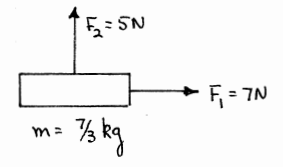
\includegraphics[scale=0.7]{forces}
    \caption{Fuerza resultante}
    \label{fig:forces}
  \end{figure}

Se escoge un sistema de coordenadas tal que
\begin{align}
  \mathbf{F}_1=&7\hat{\mathbf{i}}+0\hat{\mathbf{j}}\nonumber\\
  \mathbf{F}_2=&0\hat{\mathbf{i}}+5\hat{\mathbf{j}}\,.
\end{align}
Entonces
\begin{align}
  \mathbf{F}_R=\mathbf{F}_1+\mathbf{F}_2=
  7\hat{\mathbf{i}}+5\hat{\mathbf{j}}\,.
\end{align}
La aceleraci\'on, que esta en la misma direcci\'on que la fuerza esta dada por
\begin{align}
  \mathbf{a}=\frac{\mathbf{F}_R}{m}=\frac{7\hat{\mathbf{i}}+5\hat{\mathbf{j}}}{7/3}=3\hat{\mathbf{i}}+\frac{15}{7}\hat{\mathbf{j}}\,.
\end{align}

\item[\textbf{Ejemplo:}] Un disco plano de masa $m=\SI{2}{\kilo\gram}$, se desliza sobre un lago congelado con una rapidez inicial de $v=\SI{5}{\meter\per\second}$. La fuerza de fricci\'on tiene un valor constante de $f=\SI{4}{\newton}$ opuesta al movimiento. \textquestiondown cuan lejos avanza el disco antes de detenerse?

Escogiendo apropiadamente el sistema de coordenadas, tenemos:
\begin{align}
  -f \hat{\mathbf{i}}=m\mathbf{a}\,,
\end{align}
de donde
\begin{align}
  \mathbf{a}=-\frac{f}{m}\hat{\mathbf{i}}=\frac{-\SI{4}{\newton}}{\SI{2}{\kilo\gram}}\hat{\mathbf{i}}={-2\hat{\mathbf{i}}}{\si{\meter\per\second\squared}}\,.
\end{align}
De la cinemática del problema tenemos (eq.~\eqref{eq:trayectoriay})
\begin{align}
  v_f^2-v_0^2=2 a x\,.
\end{align}
Cuando el disco se detiene $\mathbf{v}_f=0$, de modo que
\begin{align}
  -v_0^2=&2ax\nonumber\\
  x=&-\frac{v_0^2}{2a}=\SI{6.25}{\meter}\,.
\end{align}


\end{itemize}

\subsection{Tercera Ley de Newton}
Las fuerzas siempre aparecen en pares: si un cuerpo $b$ ejerce una fuerza $\mathbf{F}_a$ en un cuerpo $a$, entonces debe haber otra fuerza $\mathbf{F}_b$ actuando en el cuerpo $b$, debido al cuerpo $a$, tal que
\begin{align}
  \mathbf{F}_b=-\mathbf{F}_a\,.
\end{align}
En otras palabras
\begin{align}
  \text{acci\'on}=-\text{reacci\'on}\,:
\end{align}
Si un cuerpo aislado sufre una aceleraci\'on y no podemos encontrar un objeto externo que sufre una aceleraci\'on igual pero opuesta, entonces estaremos en problemas. Un ejemplo mas típico de un par acción-reacción es el de dos patinadores sobre hielo intercambiando una pelota.

La segunda ley $\mathbf{F}=d\mathbf{p}/dt$,  es válida sólo en sistemas inerciales.

En general, las leyes de Newton sólo son válidas en sistemas inerciales. Entonces ¿como se puede decidir o no si un sistema es inercial?:
\begin{itemize}
\item Tome un cuerpo libre.
\item Si este permanece en un estado de movimiento uniforme, entonces se esta en un sistema inercial.
\end{itemize}

La tierra es b\'asicamente un sistema inercial en el cual la aceleración centrípeta debida a la rotación en el Ecuador es de $\SI{0.34}{\meter\per\second\squared}$

La estructura y el comportamiento del Universo entero puede ser descrito por la acción de cuatro fuerzas fundamentales descritas en la tabla~\ref{tab:forces}
\begin{table}
  \centering
  \begin{tabular}{l|cc|r}
    &Rango& Intensidad&Mediador\\\hline
Fuerza fuerte (n\'ucleos hadr\'onicos) & $10^{-15}\si{\meter}$ &1 &gluones\\
Fuerza electromagn\'etica (cargas) & $\infty$ & $10^{-2}$ & fot\'on\\
Fuerza d\'ebil &$10^{-17}\si{\meter}$&$10^{-13}$ (isosp\'\i n)& $W^\pm,\ Z^0$\\
Fuerza gravitacional (masas)&$\infty$& $10^{-38}$& gravit\'on\\
  \end{tabular}
  \caption{Fuerzas fundamentales. La intensidad se mide con respecto a la fuerza entre dos protones separados $10^{-15}\si{\meter}$}
  \label{tab:forces}
\end{table}



\section{Aplicaciones de las leyes de Newton}
\begin{frame}
El método para resolver un problema de din\'amica, consiste en
\begin{itemize}
\item Escoja un sistema, consistiendo de una porción del Universo. El resto del Universo es llamado el entorno.
\item Haga una lista de los objetos del entorno que ejercen fuerzas significativas sobre el sistema escogido. 
\item Haga un diagrama mostrando las fuerzas externas ejercidas por los objetos del entorno sobre el sistema. Esto es llamado un ``diagrama de cuerpo libre'' en el cual el efecto del entorno sobre el sistema es indicado con flechas que representan las fuerzas externas.
\item Establezca los tiempos iniciales y finales
\item Establezca las ecuaciones de movimiento de cada cuerpo
\item Identifique las fuerzas de acci\'on--reacci\'on
\item Establezca las condiciones de ligadura.
\item Comprueba unidades, compruebe la lógica de su respuesta (dirección del moméntum, cambio en la magnitud del moméntum) basado en la situación física.
\end{itemize}
\end{frame}
 

Para ilustrar estos pasos, considere el diagrama de bloques mostrado en la figura~\ref{fig:blocks}, los cuales se encuentran en reposo. Encuentre la Fuerza ejercida por el bloque $B$ sobre el $A$, y la fuerza normal de la superficie sobre el bloque $B$.


 $\mathbf{F}_A$ es la fuerza que ejerce el bloque $A$ sobre el bloque $B$, mientras que $\mathbf{F}_B$ es la fuerza que ejerce el bloque $B$ sobre $A$. De acuerdo a la tercera ley de Newton
\begin{align}
  \mathbf{F}_B=\mathbf{F}_A\,.
\end{align}
Note que la tercera ley de Newton nunca relaciona dos fuerzas actuando sobre el mismo cuerpo; las fuerzas de dos cuerpos diferentes son las que est\'an involucradas en la tercera ley. En la figura \ref{fig:blocks}: $\mathbf{N}$ representa la fuerza normal que ejerce el piso sobre el bloque $B$, mientras que $\mathbf{W}_A$ y $\mathbf{W}_B$ representan los pesos de los bloques $A$ y $B$ respectivamente. 


\begin{figure}
  \centering
  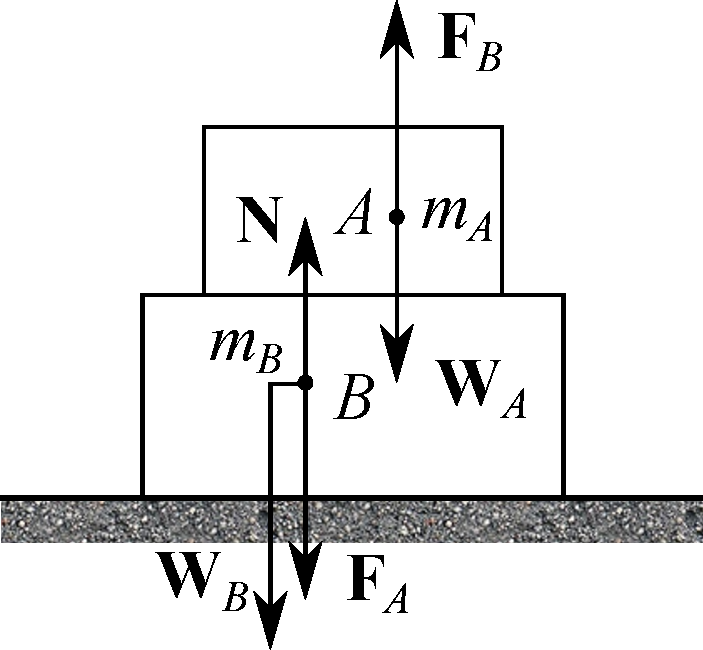
\includegraphics[scale=0.7]{blocks}
  \caption{Diagrama de fuerzas}
  \label{fig:blocks}
\end{figure}

Completando el problema de los dos bloques sobre la superficie tenemos, en la direcci\'on $\hat{\mathbf{j}}$:
\begin{align}
  \text{Ecuaciones de movimiento}&
  \begin{cases}
F_B-W_A=m_A a_A\\
N-F_A-W_B=m_B a_B\\
  \end{cases}\nonumber\\
\text{Tercera ley de Newton}\quad &F_A=F_B\nonumber\\
\text{Constraint equations}&
\begin{cases}
a_A=0\\
a_B=0\\  
\end{cases}
\end{align}
Solucionando las ecuaciones encontramos
\begin{align}
  F_B=&F_A=W_A\nonumber\\
  N=&W_A+W_B\,.
\end{align}
El objetivo principal de este ejemplo es ayudar a distinguir entre la fuerza que se aplica a un objeto 


\begin{itemize}
\item[\textbf{Ejemplo:}] Dos astronautas inicialmente en reposo en el espacio libre, tiran de ambos lados de una cuerda. La fuerza con la que el astronauta $A$ puede tirar de la cuerda, $F_A$ es mayor que la del astronauta $B$, $F_B$. Sus masas son $M_A$ y $M_B$ y la masa de la cuerda es despreciable. Encuentre el movimiento de la cuerda

Sistema: Cuerda

Entorno: Astronautas

Diagrama de cuerpo libre: (pendiente)

Ecuación de movimiento para la cuerda:
\begin{align}
  {F}_{A'}=&F_{A}\nonumber\\
  {F}_{B'}=&F_{B}
\end{align}

\begin{align}
  F_{A'}-F_{B'}=&m_{\text{cuerda}} a_{\text{cuerda}}\nonumber\\
  F_{A}-F_{B}=&m_{\text{cuerda}} a_{\text{cuerda}}\nonumber\\
\approx&0\times a_{\text{cuerda}}\nonumber\\
=&0\,,
\end{align}
de donde
\begin{align}
  F_A=F_B
\end{align}
y no hay movimiento neto de la cuerda.
\end{itemize}

\section{Ingredientes de problemas de dinámica}

\subsection{El peso}
Como hemos visto en la definción de la segundo Ley de Newton, la masa es una medidad de la resistencia que un cuerpo ofrece a los cambios en su velocidad. En la expresión para la segunda Ley de Newton con masa constante
\begin{align}
  \mathbf{F}=m_I \mathbf{a}\,,
\end{align}
$m_I$ es la masa inercial. Es el valor númerico que se obtiene al tirar un cuerpo desplazandose en una superficie sin fricción con un dinanómetro. Si simplemente se sostiene el mismo peso con un dinanómetro sobre la superficie de la tierra, obtenemos la masa gravitacional
\begin{align}
  \mathbf{F}=&m_G\mathbf{g}&\text{donde}\qquad \mathbf{g}\approx(0,-9.8,0)\ \text{m}/\text{s}^2\,,
\end{align}
Numericamente el valor de ambas masas coinciden $m=m_I=m_G$. La proporcionalidad entre masa inercial y masa gravitacional es una hipótesis en la Mecánica Newtoniana, pero es un resultado de la Teoría General de la Relatividad. Definimos entonces el peso de una partícula como el valor de la masa gravitacional por la aceleración gravitacional
\begin{align}
  |\mathbf{W}|=mg\,.
\end{align}

Hay que tener en cuenta sin embargo, que las básculas realmente miden es la fuerza normal

\subsection{Fuerza normal}
Para que un cuerpo se mantenga sobre una superficie se requiere que su peso sea compenzado por una fuerza igual y en sentido opuesto ejercida por la superficie sobre el cuerpo. Dicha fuerza se llama la fuerza normal de la superficie y se denota con la letra $\mathbf{N}$

%introducir discusion de fuerzas interatómicas

En general la fuerza normal debe incluir la presión atmosférica. Para una cuerpo con una area $A$ expuesta a la atmosféra sobre una superficie horizontal, se tendría 
\begin{align}
 N=mg+P_a A\,, 
\end{align}
donde $P_a$ es la presión atmosférica. 
\begin{itemize}
\item[\textbf{Ejemplo}] \textbf{Tortuga dentro de un ascensor}. Suponga que una tortuga, de masa $m$, está sobre una báscula dentro de un ascensor que se mueve verticalmente con una aceleración de magnitud $a_y$. Calcule la fuerza normal sobre la tortuga ejercida por la báscula. El diagrama de fuerza se muestra en la Figura (pendiente). 

La ecuación de movimiento en la dirección $y$ es (suponiendo una aceleración en la dirección $y$ positiva), con $\mathbf{N}=(0,N,0)$, $\mathbf{F}_{\text{grav}}=(0,-mg,0)$, y $\mathbf{a}=(0,a_y,0)$
\begin{align}
  N-mg=m a_y\,,
\end{align}
de modo que
\begin{align}
  N=m(g+a_y)
\end{align}
Si $a_y=0$, $N=mg$, y la báscula entrega la masa correcta para la
tortuga, sin embargo para una $a_y$ diferente de cero, la báscula
registra una ``masa'' que puede ser mayor o menor que $m$. Para
$a_y=-g$, es decir, que el ascensor se encuentra en caída libre hacia
la superficie de la tierra $N=0$, y la báscula registra un peso cero
para la tortuga. De hecho en esta situación la tortuga se encuentra en
estado de ingravidez: Un sistema cerrado (el ascensor con su contenido
interior) en caída libre en un campo gravitacional constante, es
indistinguible de un sistema con gravedad cero, es decir, el mismo
ascensor en el espacio exterior alejado de cualquier otro cuerpo.
\end{itemize}

\subsection{Cuerdas ideales}
Una cuerda ideal es inextensible y su masa es despreciable. 
\begin{itemize}
\item[\textbf{Ejemplo}] \textbf{Cuerda no ideal}
Escriba la ecuación de movimiento para una cuerda de masa $m$ sometida a tensión a ambos lados. 

La ecuación de movimiento para eje $x$ a lo largo de la cuerda es 
\begin{align*}
  \mathbf{T}_1-\mathbf{T}_2=&m\mathbf{a}\nonumber\\
  T_1-T_2=m a\,,
\end{align*}
donde $\mathbf{T}_{1,2}=(T_{1,2},0,0)$, y $\mathbf{a}=(a,0,0)$. Si la masa de la cuerda es despreciable, entonces
\begin{align*}
  T_1=T_2\,.
\end{align*}


\end{itemize}
El concepto de masa despreciable en una cuerda ideal implica que la tensión es la misma en ambos lados de la cuerda. 

\subsection{Poleas ideales}
La masa y el radio de una polea ideal son despreciables. Esto implica que las tensiones a un lado a otro de una cuerda ideal que pasa por una polea ideal son iguales en magnitud. Una polea ideal tiene entonces la propiedad de cambiar la dirección de la tensión sobre una cuerda ideal, sin alterar su magnitud.
\subsection{Aplicaciones en entornos sin fricción}







\begin{itemize}
\item[\textbf{Ejemplo:}] Tres vagones de masa $M$ están halados con una fuerza $F$ por una locomotora. Despreciando las fuerza de fricción con los rieles, encuentre las fuerzas en cada carro.
  \begin{enumerate}
  \item Sistema: Los tres vagones\\
  Entorno: los rieles y el aire\\
Diagrama: (pendiente)
  \begin{align}
    F=3M a\,,
  \end{align}
de donde
\begin{align}
  a=\frac{F}{3M}
\end{align}
\item Sistema: Primer vagón\\
Entorno: Segundo vagón, rieles, aire\\
Diagrama: (pendiente)

  \end{enumerate}
\end{itemize}
\section{Fricci\'on}

Se define como fuerza de fricción a la fuerza entre dos superficies de contacto que se opone al movimiento entre ambas superficies (\emph{fuerza de fricción dinámica}, o la fuerza que se opone al inicio del movimiento (\emph{fuerza de fricción estática}. Aunque los procesos interatómicos que dan lugar a la fuerza de fricción son muy complicados se han logrado establecer las siguientes fórmulas empíricas para la fuerza de fricción entre dos superficies

\subsection{Fricci\'on din\'amica}
\begin{align}
  \mathbf{f}=\mu_d \mathbf{N}\,,
\end{align}
donde $\mathbf{N}$, es la fuerza normal entre las superficies. El coeficiente de fricción $\mu_d$ tiene que ser menor que 1 porque de lo contrario los cuerpos se podrían subir por las paredes. 

\subsection{Fricción estática}
\begin{align}
  f>\mu_e N\,,
\end{align}
y $\mu_e$ es el coeficiete de fricción estático.




\begin{frame}
  \begin{block}%
{Ferrocarriles:} En efecto, el origen del término ferrocarril son los carriles (1) de hierro, aunque hoy en día tanto el carril como la rueda se fabrican de acero porque este material presenta unas características mecánicas más apropiadas. Además de la interesante cualidad de no tener que arreglar pinchazos (festival del humor), la principal ventaja de un transporte basado en la rodadura entre aceros es el bajo coeficiente de rozamiento que permite que un tren circulando a 100 km/h a la deriva en una vía recta y horizontal, recorra unos 10 km sin detenerse. 
  \end{block}
El coeficiente de resistencia de rodado del acero en un riel varía entre 0.0002 y 0.0010\footnote{\url{http://www.tribology-abc.com/abc/cof.htm}} 
\end{frame}

Una discusión acerca de la física de los ferrocarriles puede encontrarse en \url{http://www.jotdown.es/2012/04/el-ferrocarril-ese-gran-desconocido/}.

\begin{table}
   \centering
   \begin{tabular}{|l|c|c|}\hline
    Superficies & $\mu_e$ & $\mu_d$\\\hline
     Acero-Acero & 0.15 & 0.07\\\hline
   \end{tabular}
  \caption{Coeficientes de Fricción}
   \label{tab:coeffric}
\end{table}


\begin{itemize}
\item[Ejemplo] \textbf{Acero-Acero: Ferrocarriles} Calcule la distancia de frenado de un tren asumiendo que las ruedas dejan de rotar inmediatamente cuando se mueve a 160~Km/h.

Asumiendo que la fuerza de fricción es constante, tenemos una desaceleración constante de
\begin{align}
  a=&-\frac{f_d}{m_{\text{tren}}}=-\frac{\mu N}{m_{\text{tren}}}=-\frac{\mu m_{\text{tren}} g}{m_{\text{tren}}}=
-\mu g\,.
\end{align}
Aplicando las ecuaciones para movimiento a aceleración constante, en particular la ec.~\eqref{eq:trayectoriay}, tenemos que cuando la rapidez final es cero
\begin{align}
  v^2-v^2_0=&2 a x\nonumber\\
  -v^2_0=&2 a x\,.
\end{align}
La distancia recorrida desde el inicio del frenado es
\begin{align}
  x=&-\frac{v^2_0}{2a}\nonumber\\
 =&\frac{v_0^2}{2\mu g}\,,
\end{align}
Para $\mu_d=0.07$, tenemos $x\approx 1440\ $m.

La ley empírica de frenado de trenes es:
\begin{align}
  x=\frac{3}{2}\frac{v_0^2}{|a|}
\end{align}
donde $a$ es la desaceleración del tren, típicamente alrededor de $-2\ \text{m}/\text{s}^2$, de donde podemos obtner un estimado para el coeficiente de fricción
\begin{align*}
  \mu=\frac{|a|}{3g}=0.07\,.
\end{align*}

de donde 
\end{itemize}

\begin{itemize}
\item[\textbf{Ejemplo:}] Considere la situación ilustrada en la figura~\ref{fig:poleaideal}, donde $m_1>\mu_d m_2$. 

\begin{frame}
  \begin{figure}
    \centering
    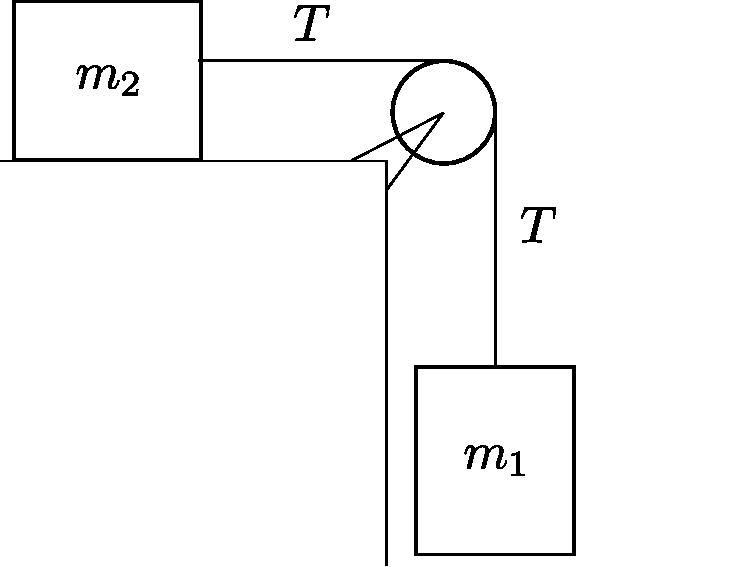
\includegraphics[scale=0.5]{poleaideal}
    \caption{Polea ideal}
    \label{fig:poleaideal}
  \end{figure}
Argumente por que la siguiente solución para la aceleración del sistema es incorrecta
\begin{align*}
      a=&\frac{g(m_1-\mu_k m_2)}{m_2-m_1}\,.
\end{align*}
\end{frame}

La condición $m_1>\mu_d m_2$  garantiza que $m_1$ cae arrastrando a $m_2$ pero con una aceleración menor que la gravedad en un factor $m_1-\mu_k m_2$. Sin embargo como $m_2$ puede ser mayor que $m_1$, la solución implicaría que el sistema se podría acelerar hacía la izquierda de $m_2$, tal que $m_1$ suba. Lo cual es claramente inconsistente. 

\end{itemize}

\section{Problemas resueltos}

\ejercicio{}
\begin{frame}
  Un jugador de baloncesto lanza un balón hacia un segundo
jugador, con una rapidez $v_0$ formando un ángulo $\theta$ por
encima de la horizontal. 
En ese instante el receptor, que está a una distancia $x_0$ adelante
del lanzador, va al encuentro del balón con cierta rapidez $v_1$
constante para atraparlo a la misma altura a la cual fue lanzado.
\begin{enumerate}
\item Haga un diagrama ilustrativo de la situación planteada, donde se muestre el sistema de referencia a emplear, la trayectoria seguida por el balón y la posición inicial del receptor.
  \label{item:1jug}
\item Plantee las ecuaciones cinemáticas de posición y velocidad que rigen el movimiento del balón y del receptor.
  \label{item:2jug}
\item Encuentre el valor de la rapidez del receptor que le permite atrapar el balón. 
  \label{item:3jug}
\item Calcule la rapidez $v_1$ hallada en el literal anterior para los valores particulares de $\theta=30^\circ$ , $v_0=\SI{20}{\meter\per\second}$  y $x_0=\SI{20}{\meter}$. De acuerdo con su resultado, ¿en qué sentido se mueve el receptor?.
  \label{item:4jug}
\end{enumerate}
\end{frame}


\subsection*{Solución}
  \begin{itemize}
  \item[~\ref{item:1jug})] Escogemos el sistema de referencia en el origen del primer jugador
  \item[~\ref{item:2jug})] Para el balón
    \begin{align*}
      y=&v_{0y}t-\frac{1}{2}gt^2\nonumber\\
      x=&v_{0x}t\,.
    \end{align*}
    Para el receptor
    \begin{align*}
      x_r=&x_0+v_1 t
    \end{align*}
  \item[~\ref{item:3jug})]
    El tiempo de vuelo $t_v$ del balón se encuentra para $y=0$
    \begin{align*}
      v_{0y}t_v=&\frac{1}{2}gt_v^2\nonumber\\
      v_{0y}=&\frac{1}{2}gt_v\,,
    \end{align*}
    de modo que
    \begin{align}
      \label{eq:tv}
      t_v=&\frac{2v_{0y}}{g}\,,
    \end{align}

    Para el tiempo de vuelo $t_v$, obtenemos el alcance
    \begin{align}
      \label{eq:13}
      R=&v_{0x}t_v \nonumber\\
       =&2 v_{0x}\frac{v_{0y}}{g} \nonumber\\
       =&\frac{2 v_{0}^2\cos\theta\sin\theta}{g} \nonumber\\
       =&\frac{v_0^2}{g}\sin(2\theta)
    \end{align}
    Para que el receptor pueda atrapar el balón, su posición con respecto al sistema de referencia después de un tiempo $t_v$ debe ser justo el alcance $R$
    \begin{align*}
      x_0+v_1 t_v=&R\nonumber\\
      v_1 t_v=&\frac{v_0^2}{g}\sin(2\theta)-x_0\nonumber\\
      2 v_1 \frac{v_{0y}}{g}=&\frac{v_0^2}{g}\sin(2\theta)-x_0\nonumber\\
      v_1 =&\left( \frac{v_0^2}{g}\sin(2\theta)-x_0 \right) \frac{g}{2v_0\sin\theta}\nonumber\\
      =&\frac{v_0^2\sin(2\theta)-gx_0}{2v_0\sin\theta}\nonumber\\
    \end{align*}

    
  \item[~\ref{item:4jug})]Evaluando la ec.~(\ref{eq:v1})
    \begin{align*}
      v_1=\SI{7.52}{\meter\per\second}
    \end{align*}

además 
\begin{align*}
t_v=&\SI{2.04}{\second}\nonumber\\
 R=&\SI{35.35}{\meter}\,
\end{align*}

y el receptor se mueve en la misma dirección del balón.\finejemplo
  \end{itemize}



\ejercicio{}
\begin{frame}
 Una cuerda ideal pasa a través de una polea ideal con uno de sus
  extremos unido al bloque 1 que cuelga sobre un lado de la mesa que
  sostiene la polea. El otro extremo de la cuerda esta unido a un
  bloque 2 que se desliza a lo largo de la mesa. Ver Figura
  \ref{fig:poleaideal}. El coeficiente de fricción cinético entre la
  masa y el bloque 2 es $\mu_d$. El bloque 1 tiene una masa $m_1$ y el
  bloque 2 tiene una masa $m_2$, con $m_1>\mu_k m_2$. En el tiempo
  $t=0$, los bloques son liberados desde el reposo y la cuerda no se
  desliza alrededor de la polea, En el tiempo $t=t_1$, el bloque 1
  golpea el piso. Encuentre la magnitud de la aceleración de cada
  bloque. Exprese su respuesta en términos de $m_1$, $m_2$, $\mu_d$. 
\end{frame}

\subsubsection*{Solución}
\begin{frame}[fragile,allowframebreaks]
\begin{itemize}
\item  \textbf{Escogencia del sistema}. Para el sistema compuesto por el bloque 2, el entorno es la mesa y la cuerda, mientras que para el sistema compuesto por el bloque 1, el entorno es la cuerda y la tierra. Además escogemos un sistema de referencia $x-y$ usual. 

\item \textbf{Diagramas de fuerzas} De acuerdo a los diagramas de cuerpo libre para ambos cuerpos ilustrado en la figura~\ref{fig:poleaidealfzas}. Tenemos
  \begin{itemize}
  \item Fuerzas en $x$ bloque 2:
  \begin{align}
    \label{eq:pi1}
    (T-{\color{red}f})\hat{\mathbf{i}}=&m_2 (a\,\hat{\mathbf{i}})\nonumber\\
    T-{\color{red}f}=&m_2 a\,.
  \end{align}
  \item Fuerzas en $y$ bloque 2:
  \begin{align}
    (N-W_2)\hat{\mathbf{j}}=&0\nonumber\\
    N-W_2=&0\nonumber\\
    N=&m_2 g\,
  \end{align}
  en adelante suprimiremos los vectores unitarios en las ecuaciones
  resultantes de los diagramas de cuerpo libre.

  \item Fuerzas en $y$ bloque 1:
  \begin{align}
    \label{eq:pi2}
    T-W_1=&{\color{blue}-}m_1 a\nonumber\\
    T-m_1 g=&{\color{blue}-}m_1 a
  \end{align}
   donde el signo menos se debe a que la aceleración está en la dirección opuesta a $y$
  \end{itemize}
\item \textbf{Establezca las condiciones de ligadura:} La relación entre la fuerza normal y la fuerza de fricción es
  \begin{align}
    \label{eq:pi3}
    {\color{red}f}=&{\color{red}\mu_d} N\nonumber\\
    =&{\color{red}\mu_d} m_2 g\,.
  \end{align}
\item \textbf{Solucine las ecuaciones:} Restando las ecuaciones \eqref{eq:pi1} y \eqref{eq:pi2}, tenemos
  \begin{align*}
    -f+m_1 g=m_2 a+m_1 a=(m_2{\color{blue}+}m_1)a\,.
  \end{align*}
Despejando $a$ y usando \eqref{eq:pi3}
\begin{align}
  \label{eq:polea}
  a=&\frac{m_1g-f}{m_2{\color{blue}+}m_1}\nonumber\\
  =&\frac{m_1g-{\color{red}\mu_d} m_2 g}{m_2{\color{blue}+}m_1}\nonumber\\
  =&\frac{m_1-{\color{red}\mu_d} m_2 }{m_2{\color{blue}+}m_1}g\\
  \le&g\nonumber\,.
\end{align}
\finejemplo
\end{itemize}
%incluir aceleración


\begin{figure}
    \centering
    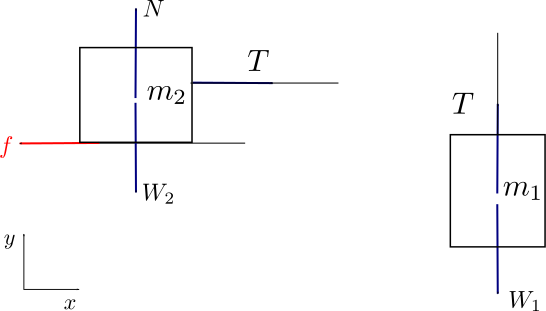
\includegraphics[scale=0.5]{poleaidealfzas}
    \caption{Diagramas de cuerpo libre ideal}
    \label{fig:poleaidealfzas}
  \end{figure}
\end{frame}
  \begin{itemize}
  \item[\textbf{Ejercicio}] Repita el problema usando un sistema de referencia rotado 90 grados en la dirección de las manecillas del reloj, para el bloque de masa $m_1$.
  \end{itemize}

\ejercicio{}

(Tomado de \cite{gabriel}) Se coloca un bloque de masa $m_1$ sobre un bloque de masa $m_2$ (como se muestra en la figura). Los coeficientes de fricción cinético y estático entre los bloques son $\mu_k$ y $\mu_e$ respectivamente. Suponer que no hay fricción entre el bloque de masa $m_2$ y la superficie sobre la cual reposa. Se aplica una fuerza $\mathbf{F}$ horizontal al bloque de masa $m_2$

  \begin{minipage}{0.4\linewidth}
    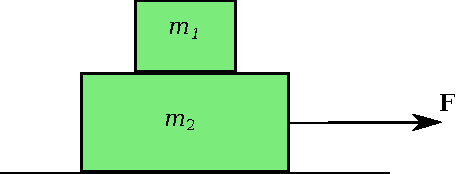
\includegraphics[scale=0.95]{bloques}
  \end{minipage}
  \begin{minipage}{0.6\linewidth}
    \begin{enumerate}
    \item Dibujar todas las fuerzas que actúan sobre cada bloque.
      \label{item:d1a}
    \item Escribir las ecuaciones de movimiento para cada bloque
      \label{item:d1b}
    \item ¿Cuál es la máxima fuerza que puede aplicarse al bloque $m_2$ de modo que los bloques se muevan juntos?
      \label{item:d1c}
    \item ¿Cual es la aceleración cuando se aplica la fuerza máxima?
      \label{item:d1d}
    \item ¿Que distancia recorren los bloques a esa aceleración durante dos segundos?
      \label{item:d1e}
    \item Evalue sus respuestas para $m_1=3\ $Kg, $m_2=5\ $Kg, $\mu_k=0.1$, $\mu_e=0.2$
      \label{item:d1f}
    \end{enumerate}
  \end{minipage}

\subsubsection*{Solución}
  \begin{itemize}
  \item[\ref{item:d1b})] Para $m_1$
    \begin{align}
      \label{eq:d11}
      m_1 a_1=&f & N_1-m_1 g=0
    \end{align}
Para $m_2$
\begin{align*}
  m_2 a_2=&F-f & N_2-N_1-m_2g=&0\,.
\end{align*}
    De modo que
    \begin{align*}
      a_1=&\frac{f}{m_1}& a_2=&\frac{F-f}{m_2}\,,
    \end{align*}
    y
    \begin{align*}
      f=\mu m_1 g\,.
    \end{align*}
  \item[\ref{item:d1c})]
    La condición de que los bloques se muevan juntos corresponde a $a_1=a_2$:
    \begin{align*}
      \frac{f}{m_1}=&\frac{F-f}{m_2}\\
      m_2 f =&m_1(F-f)\\
      m_1F =&f(m_1+m_2)\\
      m_1F =&\mu m_1 g(m_1+m_2)\\
      F =&\mu g(m_1+m_2)\,. 
    \end{align*}
    $F$ es máxima cuando $\mu=\mu_e$
    \begin{align*}
      F_{\text{max}}=\mu_e g(m_1+m_2)\,. 
    \end{align*}

    \item[\ref{item:d1d})] La aceleracíon máxima se obtiene de \eqref{eq:d11}:
      \begin{align*}
        a=\frac{f}{m_1}=\mu_e g\,.
      \end{align*}
    \item[\ref{item:d1e})] Para $t=\SI{2}{\second}$
      \begin{align*}
        x=&\frac{1}{2}a t^2
      \end{align*}
    \item[\ref{item:d1e})] $F=\SI{15.7}{\newton}$, $a=\SI{1.96}{\meter\per\second^2}$, $x=\SI{3.92}{\meter}$ \finejemplo

    \end{itemize}

\ejercicio{}
\begin{frame}[fragile,allowframebreaks]
 Dos bloques de masa $m_1$ y masa $m_2$ se mueven como lo índica la figura. Suponga que el piso es una superficie lisa (no hay fricción) y que la superficie de contacto entre los dos bloques es rugosa con coeficiente de fricción  $\mu$.

  \begin{minipage}{0.4\linewidth}
    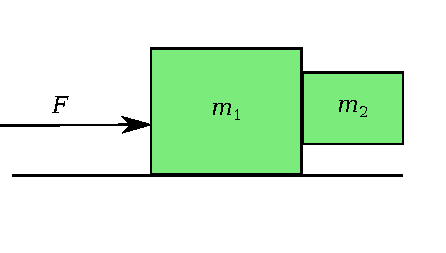
\includegraphics[scale=0.95]{bloquespegados0}
  \end{minipage}
  \begin{minipage}{0.6\linewidth}
    \begin{enumerate}
    \item Dibujar todas las fuerzas que actúan sobre cada bloque.
      \label{item:dp1a}
    \item Determine la magnitud de la fuerza mínima para que $m_2$ no se deslice. Justifique porque es mínima.
      \label{item:dp1b}
    \item Calcule dicha fuerza para $m_1=\SI{6}{\kilo\gram}$, $m_2=3\times 10^3\si{\gram}$, y $\mu=0.6$
      \label{item:dp1c}
    \end{enumerate}
  \end{minipage}
\end{frame}
\subsubsection*{Solución}
\begin{frame}[fragile,allowframebreaks]
\begin{itemize}
  \item[\ref{item:dp1a})] Recapitulemos de nuevo los pasos para solucionar los problemas de dinámica, pues en este caso son muy importantes la ecuaciones de ligadura. Primero establecemos los diagramas de cuerpo libre:
 
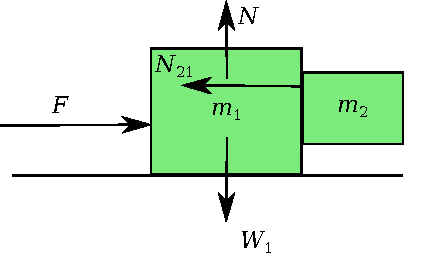
\includegraphics{bloquespegados1} 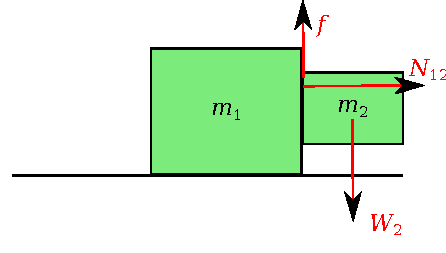
\includegraphics{bloquespegados2}

  \item[\ref{item:dp1b})] Continuamos estableciendo las ecuaciones de movimiento en forma vectorial.  


La sumatoria de fuerzas para $m_1$
    \begin{align*}
    \sum \mathbf{F}=&(F,0,0)-(N_{21},0,0)+(0,N,0)-(0,W_1,0)=(m_1 a_x,0,0)\,,  
    \end{align*}
    donde $N_{21}$ es la fuerza de reacción del bloque 2 sobre el bloque 1, de modo que la ecuación de movimiento relevante es
    \begin{align}
      \label{eq:dp1}
      F-N_{21}=&m_1 a_x\,.
    \end{align}

    Para el bloque 2 tenemos
    \begin{align*}
    \sum \mathbf{F}=&(N_{12},0,0)+(0,f,0)-(0,W_2,0)=(m_2a_x,-m_2 a_y,0)\,. 
    \end{align*}
    que da lugar a
    \begin{align}
      \label{eq:dp2}
      \sum F_x:\quad&N_{12}=m_2 a_x\nonumber\\
      \sum F_y:\quad&f-W_2=-m_2 a_y\,.
    \end{align}

    \textbf{Condiciones de ligadura}
    Para este problema podemos establecer tres condiciones de ligadura
    \begin{enumerate}
    \item $f=\mu N_{12}$, donde $N_{12}$ es la fuerza normal del bloque 1 sobre el 2.
    \item $a_y=0$, para que el bloque $m_2$ no deslice.
    \item $N_{12}=N_{21}$: los pares acción reacción son iguales en magnitud (los signos ya se tuvieron en cuenta en las respectivas ecuaciones de movimiento)
    \end{enumerate}

    Reemplazando las ecuaciones de ligadura en las ecs.~\eqref{eq:dp2}, tenemos
    \begin{align*}
      \mu N_{12}-m_2g=&0\nonumber\\
      \mu N_{21}=&m_2g\,.
    \end{align*}
    de modo que 
    \begin{align*}
    N_{21}=N_{12}=&m_2\frac{g}{\mu}\,.
    \end{align*}
    \begin{align*}
    a_x=\frac{N_{12}}{m_2}=&\frac{g}{\mu}\,.
    \end{align*}

    Reemplazando en \eqref{eq:dp1}, tenemos
    \begin{align}
      \label{eq:dp4}
      F_{\text{min}}=&N_{21}+m_1 a_x\nonumber\\
      =&m_2\frac{g}{\mu}+m_1 \frac{g}{\mu}\nonumber\\
      =&(m_1+m_2)\frac{g}{\mu}\,.
    \end{align}

    \item[\ref{item:d1b})] Evaluando numéricamente tenemos que
      \begin{align*}
        F_{\text{min}}=\SI{147}{\newton}\,.
      \end{align*}

      Como un chequeo de consistencia, podemos ver de \eqref{eq:dp4}
      \begin{align*}
        F_{\text{min}}=&(m_1+m_2)\frac{g}{\mu}\nonumber\\
        =&(m_1+m_2)a_x\,.
      \end{align*}
      de modo que el sistema completo de los dos bloques, dentro del
      cual se cancelan todas las fuerzas internas, se mueve como un
      sistema de masa $m_1+m_2$ bajo el efecto de la fuerza externa
      $F_{\text{min}}$.\finejemplo

\end{itemize}
\end{frame}
\subsubsection*{Ejercicio}
Calcule la aceleración con la que cae el bloque 2 para un determinado valor de la fuerza aplicada $F$.
% \begin{extrapage}
%   \newpage
%   \qquad
%   \newpage
% \end{extrapage}

%%% Local Variables: 
%%% mode: latex
%%% TeX-master: "mecanica"
%%% End: 


\chapter{Momentum}
La segunda  segunda ley de Newton en us forma más general puede escribirse, para una partícula de moméntum $\mathbf{p}$, como (ver ec.~(\ref{eq:28})
\begin{align}
  \mathbf{F}=\frac{d\mathbf{p}}{dt}\,.
\end{align}
Demostraremos que la ecuación anterior cuando es aplicada a un sistéma de partículas sólo contribuyen las fuerzas externas. 

\section{Dinámica de un sistema de partículas}
Considere un sistema de $N$ partículas interactuantes con masas $m_1$, $m_2$, $m_3$, $\ldots$, $m_N$. La posición de la $i$-sima partícula es $\mathbf{r}_i$, y la fuerza sobre esta es $\mathbf{F}_i$. La ecuación de movimiento de la $i$-sima partícula es
\begin{align}
  \mathbf{F}_i=\frac{d\mathbf{p}_i}{dt}
\end{align}
Las fuerza sobre la partícula $i$ puede desdoblarse en dos términos
\begin{align}
  \mathbf{F}_i=\mathbf{F}_i^{\text{int}}+\mathbf{F}_i^{\text{ext}}\,.
\end{align}
Aquí $\mathbf{F}_i^{\text{int}}$, la fuerza \emph{interna} sobre la partícula $i$, es la fuerza debida a todas las partículas dentro del sistema, y $\mathbf{F}_i^{\text{ext}}$, la fuerza externa sobre la partícula $i$, es decir la fuerza debida a fuentes externas al sistema. La ecuación de movimiento es entonces
\begin{align}
  \mathbf{F}_i^{\text{int}}+\mathbf{F}_i^{\text{ext}}=\frac{d\mathbf{p}_i}{dt}\,.
\end{align}

El resultado de sumar todas las ecuaciones de movimiento para cada una de las partículas es entonces
\begin{align}
  \label{eq:msumfi}
  \sum_{i=1}^N  \mathbf{F}_i^{\text{int}}+\sum_{i=1}^N\mathbf{F}_i^{\text{ext}}=\sum_{i=1}^N \frac{d\mathbf{p}_i}{dt}\,.
\end{align}
El segundo término corresponde a todas las fuerzas externas actuando sobre todas las partículas. Ésta es la fuerza externa total, $\mathbf{F}_{\text{ext}}$, actuando sobre el sistema
\begin{align}
 \mathbf{F}_{\text{ext}}=& \sum_{i=1}^N\mathbf{F}_i^{\text{ext}}\,.
\end{align}
El primer término en la ec.~(\ref{eq:msumfi}), es la suma de todas las fuerzas internas actuando sobre todas las partículas. De acuerdo a la tercera ley de Newton, las fuerzas entre cualquier  par de partículas son iguales y opuestas de modo que su suma es cero. Se sigue que la suma de las fuerzas entre todas las partículas también es cero, de modo que las fuerzas internas se cancelan e pares. De aquí
\begin{align}
\sum_{i=1}^N  \mathbf{F}_i^{\text{int}}=&0\,.  
\end{align}

La ec.~(\ref{eq:msumfi}) se simplifica a
\begin{align}
  \label{eq:mfext}
  \mathbf{F}_{\text{ext}}=&\sum_{i=1}^N \frac{d\mathbf{p}_i}{dt}\nonumber\\
  =& \frac{d}{dt}\sum_{i=1}^N\mathbf{p}_i\nonumber\\
 \mathbf{F}_{\text{ext}} =& \frac{d}{dt}\mathbf{P}\,,
\end{align}
donde
\begin{align}
  \mathbf{P}=\sum_{i=1}^N\mathbf{p}_i\,,
\end{align}
es el momentum total del sistema. De modo que la fuerza externa aplicada a un sistema es igual a la tasa de cambio del momentum del sistema. Esto es cierto independiente de los detalles de la interacción. $\mathbf{F}_{\text{ext}}$ podría ser una sola fuerza actuando en una sola partículas, o podría ser la resultante de muchas interacciones involucrando cada una de las partículas del sistema.

En adelante omitiremos el subíndice ext de la ec.~(\ref{eq:mfext}), de modo que
\begin{align}
  \label{eq:mfdpdt}
  \mathbf{F}=&\frac{d\mathbf{P}}{dt}\,.
\end{align}
El resultado es idéntico a la ecuación de movimiento para una sola partícula, aunque de hecho se refiere a un sistema de partículas. 


\section{Centro de masa}




Si consideremos el sistema en su totalidad con una masa
\begin{align}
  M=\sum_{i=1}^N m_i\,,
\end{align}
podemos intentar escribir la ecuación de movimiento la forma especial de masa constante
\begin{align}
    \mathbf{F}=&\frac{d\mathbf{P}}{dt}\nonumber\\
    \mathbf{F}=&\sum_{i=1}^N\frac{d\mathbf{p}_i}{dt}\nonumber\\
    \mathbf{F}=&\sum_{i=1}^N\frac{d(m_i\mathbf{v}_i)}{dt}\nonumber\\
    \mathbf{F}=&\sum_{i=1}^Nm_i\frac{d\mathbf{v}_i}{dt}\nonumber\\
    \mathbf{F}=&\sum_{i=1}^Nm_i\frac{d\dot{\mathbf{r}}_i}{dt}\,,
\end{align}
que podemos escribir en la forma
\begin{align}
  \label{eq:mcm}
  \mathbf{F}=M\ddot{\mathbf{R}}\,,
\end{align}
si
\begin{align}
  M\ddot{\mathbf{R}}=\frac{d\mathbf{P}}{dt}=&\frac{d}{dt}\sum_{i=1}^N m_i\dot{\mathbf{r}}_i\nonumber\\
=&\sum_{i=1}^N m_i\ddot{\mathbf{r}}_i\,,
\end{align}
con $\mathbf{r}_i$ el vector de posición de cada una de las partículas con respecto a un sistema de coordenadas. Entonces
\begin{align}
\label{eq:mveccm}
  \ddot{\mathbf{R}}=\frac{1}{M}\sum_{i=1}^Nm_i\ddot{\mathbf{r}}_i\,.
\end{align}
Integrando formalmente dos veces
\begin{align}
  \int_0^{\dot{\mathbf{R}}}d(\dot{\mathbf{R}})=&\frac{1}{M}
  \sum_{i=1}^N m_i\int_0^{\dot{\mathbf{r}}_i}d(\dot{\mathbf{r}}_i)\nonumber\\
  \dot{\mathbf{R}}=&\frac{1}{M}
  \sum_{i=1}^N m_i\dot{\mathbf{r}}_i\,,\nonumber\\
  \int_0^{{\mathbf{R}}}d({\mathbf{R}})=&\frac{1}{M}
  \sum_{i=1}^N m_i\int_0^{{\mathbf{r}}_i}d({\mathbf{r}}_i)\nonumber\\
  {\mathbf{R}}=&\frac{1}{M}
  \sum_{i=1}^N m_i{\mathbf{r}}_i\,.
\end{align}

Definido de esta forma $\mathbf{R}$ es un vector desde el origen de coordenadas a un punto llamado el \emph{centro de masa} del sistema. El sistema se comporta como si toda la masa está concentrada en el centro de masa y todas las fuerzas externas actuaran sobre ese punto.

Muchas veces estamos interesado en el movimiento de cuerpos relativamente rígidos como pelotas o automóviles. Cuerpos de esta índole, corresponde a sistemas de partículas que están fijas entre sí por fuertes fuerzas externas. La ec.~(\ref{eq:mveccm}) muestra que con respecto a fuerzas externas, el cuerpo se comporta como si fuera una partícula virtual. En el capítulo~\ref{cha:dinamica}, casualmente tratamos cada cuerpo como si fuesen partículas; vemos ahora que esto esta justificado con tal de centremos nuestra atención en el movimiento del centro de masa. 

La ecuación~(\ref{eq:mcm}) es solo válida para estudiar la traslación del centro de masa. En ausencia de fuerzas externas, la aceleración del centro de masa: $\ddot{\mathbf{R}}=0$, es decir, el centro de masa se mueve a velocidad constante. Esta ley de conservación proviene de la invarianza de los sistemas bajo transformaciones de Galileo

Ilustración del movimiento de centro de masa: \url{http://www.wired.com/wiredscience/2011/09/modeling-a-falling-slinky/}. Simulación y código  \href{http://www.wired.com/wiredscience/2011/10/more-slinky-physics/}{con una pelota de tenis en el extermo}

\begin{itemize}
\item[\textbf{Ejemplo:}] Calcule el centro de masa de masa de un par de esferas de masa $m_1$ y $m_2$ unidas por una varilla de masa despreciable.
  \begin{align}
    \label{eq:mbaton}
    \mathbf{R}=\frac{m_1\mathbf{r}_1+m_2\mathbf{r}_2}{m_1+m_2}
  \end{align}
Note que la línea que une los extremos de los vectores de posición $\mathbf{r}_1$ y $\mathbf{r}_2$ corresponde a la diferencia $\mathbf{r}_1-\mathbf{r}_2$. Para comprobar que $\mathbf{R}$ se encuentra sobre esa línea,
sea el desplazamiento desde la punta de $\mathbf{R}$ hasta la punta $\mathbf{r}_1$ el vector $\mathbf{r}_1'$. De la misma forma, sea $\mathbf{r}_2'$ el vector de desplazamiento entre los extremos de $\mathbf{R}$ y $\mathbf{r}_2$. Entonces
\begin{align}
  \mathbf{r}_1'=&\mathbf{r}_1-\mathbf{R}\nonumber\\
  \mathbf{r}_2'=&\mathbf{r}_2-\mathbf{R}\,.
\end{align}
De la ec.~(\ref{eq:mbaton})
\begin{align}
  \mathbf{r}_1'=&\mathbf{r}_1-\mathbf{R}\nonumber\\
  =&\mathbf{r}_1-\frac{m_1\mathbf{r}_1+m_2\mathbf{r}_2}{m_1+m_2}\nonumber\\
    =&\frac{\mathbf{r}_1(m_1+m_2)-m_1\mathbf{r}_1-m_2\mathbf{r}_2}{m_1+m_2}\nonumber\\
    =&\frac{m_2}{m_1+m_2}(\mathbf{r}_1-\mathbf{r}_2)\,,
\end{align}
de modo que el vector $\mathbf{r}_1$ es paralelo a la varilla que une las dos esferas determinada por $\mathbf{r}_1-\mathbf{r}_2$. Similarmente
\begin{align}
  %faltan detalles
 \mathbf{r}_2'=-\left(\frac{m_1}{m_1+m_2} \right)\left(\mathbf{r}_1-\mathbf{r}_2 \right)\,.
\end{align}
De modo que tanto $\mathbf{r}_1'$ como $\mathrm{r}_2'$ yacen sobre la línea que une $m_1$ y $m_2$. Además, si la longitud de dicha línea es $l$
\begin{align}
  r_1'=&\frac{m_2}{m_1+m_2}l\nonumber\\
  r_2'=&\frac{m_1}{m_1+m_2}l\,.
\end{align}

Asumiendo que la fricción es despreciable, la fuerza externa sobre el cuerpo cuando es lanzado al aire es
\begin{align}
  \mathbf{F}=m_1\mathbf{g}+m_2\mathbf{g},
\end{align}
donde
\begin{align}
  \mathbf{g}=-g\hat{\mathbf{j}}\,.
\end{align}
La ecuación de movimiento para el centro de masa es:
\begin{align}
  \left(m_1+m_2 \right)\ddot{\mathbf{R}}=\left(m_1+m_2 \right)\mathbf{g}\,,
\end{align}
o
\begin{align}
  \ddot{\mathbf{R}}=\mathbf{g}\,.
\end{align}
El centro de masa sigue la trayectoria parabólica de una sola masa.
\end{itemize}

Para cuerpos continuos es más conveniente hacer una integral:
%faltan detalles
\begin{align}
  \mathbf{R}=\frac{1}{M}\int \mathbf{r} dm\,.
\end{align}

Para visualizar esta integral, piense $dm$ como las masa en un elemento de volumen $dV$ localizada en la posición $\mathbf{r}$. Si la densidad de masa del elemento es $\rho$, entonces $dm=\rho\,dV$, y
\begin{align}
\label{eq:mintvol}
  \mathbf{R}=\frac{1}{M}\int_V \mathbf{r}\,\rho\,dV\,, 
\end{align}
donde
\begin{align}
  \mathbf{r}=x\hat{\mathbf{i}}+y\hat{\mathbf{j}}+z\hat{\mathbf{k}}\,.
\end{align}
La integral en (\ref{eq:mintvol}), es llamada una integral de volumen.

\begin{itemize}
\item[\textbf{Ejemplo}] \textbf{Centro de masa de una varilla no uniforme}: Calcular el centro de masa de una varilla de densidad lineal $\lambda=\lambda_0(x/L)$, donde $L$ es la longitud de la varilla
  \begin{align}
    \mathbf{R}=&\frac{1}{M}\int \mathbf{r}\lambda\,dx\,.
  \end{align}
Teniendo en cuenta que
\begin{align}
  \mathbf{r}=&(x,0,0)\nonumber\\
  \mathbf{R}=&(R_x,0,0)\,,
\end{align}
tenemos que
\begin{align}
  \label{eq:m38}
  R_x=&\frac{1}{M}\int_0^L x\lambda(x)dx\nonumber\\
  =&\frac{1}{M}\frac{\lambda_0}{L}\int_0^L x^2\,dx\,.
\end{align}
Debemos calcular $M$:
\begin{align}
  M=\int dm=\frac{\lambda_0}{L}\int_0^L x\,dx=\frac{\lambda_0}{L}
  \left.\frac{x^2}{2}  \right|_0^L=\frac{\lambda_0}{2}L\,.
\end{align}
Reemplazando en \eqref{eq:m38}
\begin{align}
  R_x=&\frac{2}{\lambda_0L}\frac{\lambda_0}{L}\int_0^L x^2\,dx\nonumber\\
  =&\frac{2}{L^2}\left.\frac{x^3}{3}  \right|_0^L\nonumber\\
  =&\frac{2}{L^2}\frac{L^3}{3}\nonumber\\
  =&\frac{2}{3}L\,.
\end{align}

\item[\textbf{Ejemplo}] \textbf{Centro de masa de una hoja triangular} 
\end{itemize}

\section{Conservación del momentum}
Para un sistema aislado, es decir, un sistema que no interactúa con sus alrededores se tiene que $\mathbf{F}=0$, y por lo tanto
\begin{align}
  \frac{d\mathbf{P}}{dt}=0\,.
\end{align}
De modo que el momentum total es constante, sin importar que tan fuerte son las interacciones internas, y sin importar lo complicado del movimiento. Esta es la ley de conservación del momentum.

\begin{itemize}
\item[\textbf{Ejemplo}] \textbf{Retroceso de un cañón de resorte}\\
Un cañón de resorte cargado, inicialmente en reposo en una superficie horizontal sin fricción, dispara una canica con un ángulo de elevación $\theta$. La masa del cañón es $M$, la masa de la canica es $m$, y la velocidad de salida de la canica es $v_0$ relativa al cañón. ¿Cual es la velocidad final del cañon?

Considere el sistema como compuesto por el cañón más la canica. Como la gravedad y la fuerza son verticales no existen fuerzas horizontales en la dirección $x$, de modo que
\begin{align}
  \frac{d P_x}{dt}=0,.
\end{align}
Como $P_x$ se conserva:
\begin{align}
  P_{x,\text{inicial}}=P_{x,\text{final}}
\end{align}
Sea el tiempo inicial anterior a disparar el cañón. Entonces $P_{x,\text{inicial}}=0$, ya que el sistema está inicialmente en reposo. Después de que la canica ha abandonado la boca del cañón, el cañón retrocede con alguna rapidez $V_f$, y su momentum final es $M V_f$ hacia la izquierda. La velocidad de la canica relativa a la  mesa es $v_0\cos\theta-V_f$. Por conservación del momentum horizontal, tenemos por consiguiente que
\begin{align}
  0=m(v_0\cos\theta-V_f)-M V_f\,,
\end{align}
o
\begin{align}
  V_f=\frac{m v_0\cos\theta}{M+m}\,.
\end{align}

\end{itemize}

\begin{itemize}
\item[\textbf{Ejemplo}] \textbf{Rebote de pelota de goma}
\end{itemize}

\section{Sistemas de masa variable}
Para este tipo de sistemas se debe usar
\begin{align}
  \mathbf{F}=\frac{d\mathbf{P}}{dt}\,.
\end{align}

Para analizar este tipo de sistemas es esencial tratar con el mismo conjunto de partículas a través de todo el intervalo temporal desde el tiempo inicial al tiempo final; debemos rastrear todas las partícula que estaban originalmente en el sistema. Consecuentemente, la masa del sistema no puede cambiar durante el intervalo de interés. En el caso de un cohete, el sistema está compuesto por el cohete en sí, y el combustible que tenga al momento inicial. 



Considere un cohete a un tiempo $t$ que se mueve a velocidad $\mathbf{v}$. Entre un tiempo $t$ y $t+\Delta t$, una masa de combustible $\Delta m$ es quemada y expulsada como gas a una velocidad $\mathbf{u}$ relativa al cohete.

El sistema consiste de $\Delta m$ más la masa remanente del cohete $M$. De aquí que la masa total es $M+\Delta m$.

La velocidad del cohete al tiempo $t$ es $\mathbf{v}(t)$, y en $t+\Delta t$, es $\mathbf{v}+\Delta\mathbf{v}$. Similarmente, la velocidad de la masa de combustible al tiempo $t$ es $\mathbf{v}(t)$, y al tiempo $t+\Delta t$, es la velocidad del cohete a ese tiempo, más la suma vectorial de su propia velocidad: $\mathbf{v}+\Delta\mathbf{v}+\mathbf{u}$. 

El momentum inicial es:
\begin{align}
  \mathbf{P}(t)=(M+\Delta m)\mathbf{v}\,,
\end{align}
y el momentum final es
\begin{align}
  \mathbf{P}(t+\Delta t)=M(\mathbf{v}+\Delta\mathbf{v})+\Delta m(\mathbf{v}+\Delta\mathbf{v}+\mathbf{u})\,.
\end{align}
El cambio en el momentum es
\begin{align}
  \Delta\mathbf{P}=&\mathbf{P}(t+\Delta t)-\mathbf{P}(t)\nonumber\\
=&M\Delta\mathbf{v}+(\Delta m)(\Delta\mathbf{v})+(\Delta m)\mathbf{u}\nonumber\\
\approx &M\Delta\mathbf{v}+(\Delta m)\mathbf{u}\,,
\end{align}
donde hemos despreciado el producto de términos pequeños. Por consiguiente
\begin{align}
  \frac{d\mathbf{P}}{dt}=&\lim_{\Delta t\to 0}\frac{\Delta\mathbf{p}}{\Delta t}\nonumber\\
=&M\frac{d\mathbf{v}}{dt}+\mathbf{u}\frac{dm}{dt}\,.
\end{align}
$dm/dt$ es la tasa de cambio de la masa expulsada. Ya que esta masa proviene del cohete
\begin{align}
  \frac{dm}{dt}=-\frac{dM}{dt}\,,
\end{align}
y
\begin{align}
  \frac{d\mathbf{P}}{dt}=M\frac{d\mathbf{v}}{dt}-\mathbf{u}\frac{dM}{dt}\,.
\end{align}
como
\begin{align}
  \mathbf{F}=\frac{d\mathbf{P}}{dt},,
\end{align}
entonces
\begin{align}
  \label{eq:mrocket}
   \mathbf{F}_{\text{ext}}=M\frac{d\mathbf{v}}{dt}-\mathbf{u}\frac{dM}{dt}\,.
\end{align}

\subsection{Cohete en el espacio libre}

En el espacio exterior en ausencia de gravedad no hay fuerzas externas actuando sobre el cohete, de modo que $\mathbf{F}=0$ y la ecuación de movimiento~(\ref{eq:mrocket}) esta dada por
\begin{align}
\label{eq:m40}
  \mathbf{F}_{\text{ext}}=0\Longrightarrow M\frac{d\mathbf{v}}{dt}=\mathbf{u}\frac{dM}{dt}\,,
\end{align}
Definimos la fuerza de empuje del cohete como
\begin{align}
  \label{eq:m39}
  \mathbf{F}_E=M\frac{d\mathbf{v}}{dt}=\mathbf{u}\frac{dM}{dt}\,.
\end{align}

La ec.~\eqref{eq:40} puede reescribirse como
\begin{align}
  \label{eq:m41}
  \frac{d\mathbf{v}}{dt}=\mathbf{u}\frac{1}{M}\frac{dM}{dt}\,.
\end{align}


Generalmente la velocidad de expulsión $\mathbf{u}$ es constante, en tal caso es fácil integrar la ecuación de movimiento:
\begin{align}
{d\mathbf{v}}=\mathbf{u}\frac{dM}{M}\,.
\end{align}
La antiderivada de $1/x$ es $\ln x$, ya que
\begin{align}
  \frac{d}{dx}\ln x=\frac{1}{x},.
\end{align}
Entonces
\begin{align}
  \int_{\mathbf{v}_0}^{\mathbf{v}_f}{d\mathbf{v}}=&\mathbf{u}\int_{M_0}^{M_f}\frac{dM}{M}\nonumber\\
\mathbf{v}_f-\mathbf{v}_0=&\mathbf{u}\ln M\left|_{{}_{M_0}}^{{}^{M_f}}\right.\nonumber\\
=&\mathbf{u}\left(\ln M_f-\ln M_0\right)\nonumber\\
=&\mathbf{u}\ln\frac{M_f}{M_0}\nonumber\\
=&-\mathbf{u}\ln\frac{M_0}{M_f}\,.
\end{align}

Si $\mathbf{v}_0=0$, entonces
\begin{align}
  \mathbf{v}_f=&-\mathbf{u}\ln\frac{M_0}{M_f}\,.
\end{align}
La velocidad final es independiente de como la masa es liberada. Las únicas cantidades importante son las velocidades de expulsión y el cociente entre las masas finales e iniciales.

\begin{itemize}
\item[\textbf{Ejemplo}]Si un cohete de masa $M=\unit{1000}{\kilo\gram}$ está expulsando gas a una tasa de $\unit{10}{\kilo\gram\per\second}$, y a una velocidad de expulsión de $\unit{500}{\meter\per\second}$. Calcule la velocidad después de $\unit{20}{\second}$.\\
Después de $\unit{20}{\second}$ el cohete a expulsado una masa de $\unit{10}{\kilo\gram\per\second}\timesm\unit{20}{\second}=\unit{200}{\kilo\gram}$, de modo que $M_f=\unit{1000}{\kilo\gram}-\unit{200}{\kilo\gram}=\unit{800}{\kilo\gram}$, entonces
\begin{align}
  v_f=(-\unit{500}{\meter\per\second})\ln\frac{800}{1000}=\unit{112}{\meter\per\second}\,.
\end{align}
Del enunciado del problema se puede 
\begin{align}
  \frac{dM}{dt}=-10\ \frac{\text{Kg}}{\text{s}}\,,
\end{align}
donde el signo menos indica que la masa total del sistema cohete--combustible esta disminuyendo con el tiempo. Integrando entre un tiempo $t_i=0$ y un tiempo final $t$, tenemos
\begin{align}
  \int_0^t dM&=-10\int_0^t\nonumber\\
  M(t)&=-M(0)-10 t
\end{align}
Usando el valor para la masa inicial $M(0)=\unit{1000}{\kilo\gram}$, tenemos
\begin{align}
  M(t)=\unit{(1000-10t)}{\kilo\gram}
\end{align}
Usando la ec.~\eqref{eq:m39} podemos calcular el empuje del cohete:
\begin{align}
  \mathbf{F}_E=\mathbf{u}\frac{dM}{dt}=&\mathbf{u}(-10)\nonumber\\
  =&(-500)\timesm(-10)\hat{\mathbf{i}}\nonumber\\
  =&{5000}{\newton}\,\hat{\mathbf{i}}\,,
\end{align}
y  el empuje producido por el cohete es de ${5000}{\newton}$,  
\end{itemize}

%\begin{inprogress}
%http://mypages.iit.edu/~smart/acadyear/rockets.htm
y la aceleración
\begin{align}
  \mathbf{a}=&\frac{\mathbf{F}_E}{M(t)}\nonumber\\
  =&\unit{\frac{5000}{1000-10t}}{\meter\per\second\squared}\,\hat{\mathbf{i}}\nonumber\\
  =&\unit{\frac{500}{100-t}}{\meter\per\second\squared}\,\hat{\mathbf{i}}
\end{align}
de modo que
\begin{align}
  \textbf{v}=\unit{[-500\ln(-100+t)]}{\meter\per\second}\,\hat{\mathbf{i}}
\end{align}
\begin{align}
 \mathbf{x}=\unit{\{-500 [-t+t \ln (t-100)-100 \ln (100-t)]\}}{\meter}\,\hat{\mathbf{i}}
\end{align}
%\end{inprogress}


Si el cohete está en presencia de un campo gravitacional constante (cerca a la superficie de la tierra), la fuerza externa es
\begin{align}
  \mathbf{F}=M\mathbf{g}
\end{align}
y de \eqref{eq:mrocket}
\begin{align}
     M\mathbf{g}=M\frac{d\mathbf{v}}{dt}-\mathbf{u}\frac{dM}{dt}\,,
\end{align}
de donde
\begin{align}
  \frac{d\mathbf{v}}{dt}=\frac{\mathbf{u}}{M}\frac{dM}{dt}+\mathbf{g}\,.
\end{align}
Integrando como en la ec.~\eqref{eq:m41}
\begin{align}
   \int_{\mathbf{v}_0}^{\mathbf{v}_f}{d\mathbf{v}}=&
   -\mathbf{u}\ln\frac{M_0}{M_f}+\mathbf{g}(t_f-t_0)
\end{align}






\section{Impulso}
Definimos el impulso de una fuerza $\mathbf{F}$, durante un intervalo suficientemente pequeño $\Delta t=t_b-t_a$, como
\begin{align}
   \mathbf{I}=\mathbf{F}\Delta t=&\mathbf{P}(t_b)-\mathbf{P}(t_a)\,.
\end{align}

\subsection{Transporte de momomentum}

Considere un chorro de partículas de masa $m$ y separación $l$
%ver notas en cuaderno estrellitas

%%% Local Variables: 
%%% mode: latex
%%% TeX-master: "mecanica"
%%% End: 


\chapter{Trabajo y Energía}
\label{chap:energia}

Hasta ahora hemos explotado la homogeneidad del espacio que da lugar a la conservación de las tres componentes de la cantidad de movimiento. En este capítulo ilustraremos de nuevo el Teorema de Noether mostrando que la cantidad conservada asociada a la homogeneidad del tiempo es la \emph{Energía}. 

La homogeneidad de las ecuaciones de movimiento con respecto al tiempo queda manifiesta cuando estás se reescriben de una forma independiente del tiempo. 
 
En el caso de caída libre integramos la ecuación de movimiento para una fuerza constante $\mathbf{F}=-m g\hat{\mathbf{j}}$:
\begin{align}
  \frac{d^2y}{dt^2}=-g\,,
\end{align}
para encontrar la velocidad y la posición en función del tiempo. A partir de dichas ecuaciones encontramos la ecuación de la trayectoria \eqref{eq:trayectoriay}
\begin{align}
\label{eq:trayl}
  v^2-v_0^2=-2g(y-y_0)\,.
\end{align}

En general, es posible integrar directamente la ecuación de movimiento para obtener la ecuación de la trayectoria si consideramos la fuerza dependiendo de la posición en lugar del tiempo.

Para analizar la trayectoria de un movimiento bajo una fuerza arbitraria debemos mirar como cambia su vector de velocidad, o equivalentemente su vector de desplazamiento $\Delta\mathbf{r}$. El $v^2$ provendrá del producto escalar $\mathbf{F}\cdot \Delta\mathbf{r}$, donde
\begin{align}
  \mathbf{F}\Delta t\approx \Delta\mathbf{p}\,.
\end{align}

\section{Movimiento en una dimensión}
En el caso de masa constante, podemos escribir la ecuación de movimiento en una dimensión como
\begin{align*}
  F=&m a \nonumber\\
  F=& m \frac{dv}{dt} \nonumber\\
  Fdx=& m \frac{dv}{dt} dx = m \frac{dv}{dt}\frac{dx}{dt} dt = m v\frac{dv}{dt} dt \nonumber\\
  Fdx=& m v\, dv\,,
\end{align*}
e integrando directamente con respecto en la dirección de movimiento, asumiendo que ésta es a lo largo de $x$, tenemos que
\begin{align}
\label{eq:tray1d}
\int_{x_0}^x F dx =&m\int_{v_0}^v v dv  \nonumber\\
=&\frac{1}{2}m \left( v^2-v_0^2 \right)
\end{align}
Para el caso de $F=-mg$ y la dirección en $y$, la ecuación general de la trayectoria para un sistema de masa constante (\ref{eq:tray1d}) da lugar inmediatamente a la ec.~(\ref{eq:trayl}).


\section{Integral de línea}
A modo de teorema establecemos que la ecuación de la trayectoria para una partícula de masa constante, se puede determinar de la ecuación de movimiento  en tres dimensiones
\begin{align*}
  \mathbf{F}=m\mathbf{a}=m \frac{d\mathbf{v}}{dt}
\end{align*}
cuando se realiza la \emph{integral de línea} a lo largo de la curva continua $C$ que sigue la partícula:
\begin{align}
\label{eq:flinea}
   \int_C\mathbf{F}(\mathbf{r})\cdot d\mathbf{r}=&m\int_C\frac{d\mathbf{v}}{dt}\cdot d\mathbf{r}
\end{align}
donde la integral de línea se puede evaluar si conocemos como cambia el argumento, $\mathbf{r}$, del una función vectorial $\mathbf{G}$, en términos de algún parámetro $t$:
\begin{align}
  \label{eq:e12}
  \int_C \mathbf{G}(\mathbf{r})\cdot\,d\mathbf{r} = \int_{t_a}^{t_b} \mathbf{G}(\mathbf{r}(t))\cdot\frac{d\mathbf{r(t)}}{dt}\,dt.
\end{align}
donde $\mathbf{r}$ es el vector de posición desde un origen de coordenadas a cada uno de los segmento $d\mathbf{r}$ tangenciales a la trayectoria $C$, tal que $\mathbf{r}_a=\mathbf{r}(t_a)$ y $\mathbf{r}_b$ corresponden a las posiciones de los extremos de $C$. Aquí $\mathbf{G}(\mathbf{r})$ es una función vectorial general. Para visualizar la integral de línea, se divide la trayectoria desde la posición inicial $\mathbf{r}_a$ hasta la posición final $\mathbf{r}_b$ en $N$ segmentos cortos de longitud $\Delta \mathbf{r}_j$, donde $j$ es un índice que numera los segmentos.  Ver fig~\ref{fig:lineint}.

\begin{frame}
\begin{figure}
  \centering
  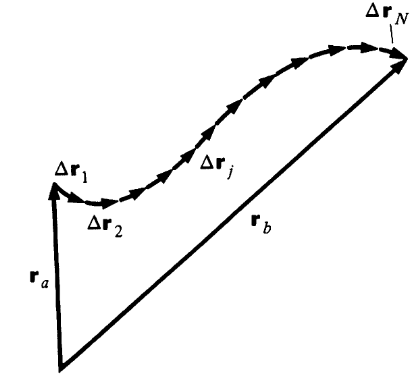
\includegraphics[scale=0.5]{lineint}
  \caption{Integral de línea}
  \label{fig:lineint}
\end{figure}
\end{frame}

Si $\Delta \mathbf{r}_j$ es suficientemente pequeño, el integrando del lado derecho de la ec.~\eqref{eq:flinea} puede escribirse como
\begin{align}
  \label{eq:dW}
  \mathbf{F}(\mathbf{r}_j)\cdot\Delta\mathbf{r}_j
\end{align}

Si $\Delta t$ es el tiempo que se tarda en atravesar un segmento, entonces
\begin{align}
  \Delta\mathbf{r}_j = \mathbf{r}(t_j+\Delta t)-\mathbf{r}(t_j)=\frac{\Delta\mathbf{r}}{\Delta t}\Delta t\,,
\end{align}
\begin{align}
  \int_C \mathbf{F}(\mathbf{r})\cdot\,d\mathbf{r}=&\lim_{\Delta t\to 0}\sum_{j=1}^N\mathbf{F}(\mathbf{r}_j)\cdot\frac{\Delta\mathbf{r}}{\Delta t}\Delta t\nonumber\\
=&\int_{t_a}^{t_b}\mathbf{F}(\mathbf{r}(t))\cdot\frac{d\mathbf{r(t)}}{dt}\,dt\,.
\end{align}
\begin{inprogress}
  Ejemplos de integrales de Línea para fuerzas constantes y centrales.
\end{inprogress}


\section{Ecuación de la trayectoria}

Aplicando el concepto de integral de línea a la ecuación de movimiento con masa constante
\begin{align}
\label{eq:trayectoria}
  \mathbf{F}(\mathbf{r})=&m\frac{d\mathbf{v}}{dt}\nonumber\\
  \int_C\mathbf{F}(\mathbf{r})\cdot d\mathbf{r}=&m\int_C\frac{d\mathbf{v}}{dt}\cdot d\mathbf{r}\nonumber\\
 \int_{t_a}^{t_b}\mathbf{F}(\mathbf{r})\cdot \frac{d\mathbf{r}}{dt}\,dt=&m\int_{t_a}^{t_b}\frac{d\mathbf{v}}{dt}\cdot \frac{d\mathbf{r}}{dt}\,dt\,.
\end{align}

Analicemos primero el caso del movimiento bajo una fuerza $F(x)$ en una dimensión. La ec.~\eqref{eq:trayectoria} queda
\begin{align}
  \label{eq:1dt}
 \int_{t_a}^{t_b}F(x)\frac{dx}{dt}\,dt=&m\int_{t_a}^{t_b}\frac{dv}{dt}\frac{dx}{dt}\,dt\nonumber\\\, 
 =&m\int_{t_a}^{t_b}\frac{dv}{dt}v\,dt\nonumber\\\, 
 =&m\int_{t_a}^{t_b}v\,\frac{dv}{dt}dt\,.
\end{align}
Realizando el cambio de variables
\begin{align}
  t\to&x(t) & t\to&v(t)\nonumber\\
 t_a\to& x(t_a)=x_a& t_a\to& v(t_a)=v_a\nonumber\\
 t_b\to& x(t_b)=x_b& t_b\to& v(t_b)=v_b\nonumber\\
 \frac{dx}{dt}dt\to& dx& \frac{dv}{dt}dt\to&dv\,,
\end{align}
y reemplazando en \eqref{eq:1dt}
\begin{align}
  \label{eq:1dtn}
 \int_{x_a}^{x_b}F\,{dx}=&m\int_{v_a}^{v_b}v\,{dv}\nonumber\\
 =&\left.\frac{1}{2}mv^2\right|_{v_a}^{v_b}\nonumber\\
=&\tfrac{1}{2}mv_b^2-\tfrac{1}{2}mv_a^2\,.
\end{align}
Definimos:
\begin{align}
  \label{eq:K}
  K\equiv&\frac{1}{2}m v^2\nonumber\\
  W_{a b}\equiv&\int_{x_a}^{x_b}F(x)dx\,,
\end{align}
donde $K$ es la \emph{energía cinética}, y $W_{a b}$ es el \emph{trabajo} hecho por la fuerza $F$ sobre la partícula a medida que ésta se mueve de $a$ a $b$. Entonces la ec.~(\ref{eq:1dtn}) queda
\begin{align}
    W_{ba}=K_b-K_a\,.
\end{align}




En el caso general de tres dimensiones, el lado derecho de la ec.~\eqref{eq:trayectoria} se puede evaluar directamente
\begin{align}
  \int_C\frac{d\mathbf{v}}{dt}\cdot d\mathbf{r}
 =&\lim_{\Delta t\to 0}\sum_{j=1}^N\frac{d\mathbf{v}}{dt}\cdot\frac{\Delta\mathbf{r}}{\Delta t}\Delta t\,.
\end{align}
Para un segmento suficientemente corto, $\mathbf{v}$ es aproximadamente constante. De aquí que $\Delta\mathbf{r}=\mathbf{v}\Delta t$, por consiguiente
\begin{align}
    \int_C\frac{d\mathbf{v}}{dt}\cdot d\mathbf{r}
    =&\int_{t_a}^{t_b}\frac{d\mathbf{v}}{dt}\cdot\mathbf{v}dt\nonumber\\
    =&\int_{t_a}^{t_b}\frac{1}{2}\left(\mathbf{v}\cdot\frac{d\mathbf{v}}{dt}+\frac{d\mathbf{v}}{dt}\cdot\mathbf{v}\right)dt\nonumber\\
    =&\int_{t_a}^{t_b}\frac{1}{2}\frac{d}{dt}\left(\mathbf{v}\cdot\mathbf{v}\right)dt\nonumber\\
    =&\int_{t_a}^{t_b}\frac{1}{2}\frac{d}{dt}(v^2)\,dt\,.
\end{align}
Como la antiderivada de $v^2$ es justamente $d(v^2)/dt$, entonces
\begin{align}
  \int_C\frac{d\mathbf{v}}{dt}\cdot d\mathbf{r}
  =&\int_{t_a}^{t_b}\frac{1}{2}\frac{d}{dt}(v^2)\,dt\nonumber\\
  =&\left.\frac{1}{2}v^2\right|_{t_a}^{t_b}\nonumber\\
  =&\tfrac{1}{2}v(t_b)^2-\tfrac{1}{2}v(t_a)^2\nonumber\\
  =&\tfrac{1}{2}v_b^2-\tfrac{1}{2}v_a^2\,.
\end{align}
y reemplazando en la ecuación para la trayectoria~\eqref{eq:trayectoria}
\begin{align}
  \label{eq:linev2}
    \int_C\mathbf{F}(\mathbf{r})\cdot d\mathbf{r}=&m\int_C\frac{d\mathbf{v}}{dt}\cdot d\mathbf{r}\nonumber\\
  =&\tfrac{1}{2}mv_b^2-\tfrac{1}{2}mv_a^2\,.
\end{align}

\section{Teorema de Trabajo-Energía}
El trabajo hecho por una fuerza $\mathbf{F}$ sobre una partícula que se mueve de $a$ hasta $b$, se define como
\begin{align}
  W_{ba}=\int_C\mathbf{F}\cdot d\mathbf{r}\,.
\end{align}
La ecuación (\ref{eq:linev2}) toma ahora la forma
\begin{align}
  \label{eq:tte}
  W_{ba}=K_b-K_a\,.
\end{align}
donde $K$ es la energía cinética de la partícula de masa $m$ y una rapidez $v$ y esta dada por la ec.~\eqref{eq:K},
\begin{align*}
  K=\tfrac{1}{2}m v^2\,.
\end{align*}



Para un sistema extendido
\begin{align}
  \int_C \mathbf{F}\cdot d\mathbf{R}=\tfrac{1}{2}M V_b^2-\tfrac{1}{2}M V_a^2\,,
\end{align}
donde $d\mathbf{R}=\mathbf{V}dt$ es el desplazamiento del centro de masa en un tiempo $t$.


\section{Cálculo del trabajo}
En el caso de movimiento en una dimensión
\begin{align*}
  \mathbf{F}=(F_x,0,0)
\end{align*}
la integral de línea se reduce a una integral normal
\begin{align*}
  \int_{\text{1-dim}}\mathbf{F}\cdot d\mathbf{R}=\int_{x_0}^{x}F_x(x)\,dx\,.
\end{align*}


\subsection{Fuerza gravitacional constante}
\begin{frame}
Considere el trabajo que tiene que realizar la fuerza gravitacional
para reducir la rapidez de una partícula que ha sido lanzada hacia
arriba con rapidez $v_0$ hasta una rapidez $v$. Tomando el origen de coordenadas en la superficie de la tierra, tenemos
\begin{align*}
  \mathbf{F}=&(0,-mg,0)\nonumber\\
  d\mathbf{r}=&(dx,dy,dz)\,.
\end{align*}
entonces
\begin{align*}
  W_{ba}=-mg\int_{y_0}^ydy=-mg(y-y_0)<0\,.
\end{align*}
y usando la ecuación (\ref{eq:linev2})
\begin{align}
  \label{eq:consrven}
  mgy_0-mgy=\tfrac{1}{2}m v^2-\tfrac{1}{2}m v_0^2\,,
\end{align}
\end{frame}
de donde
\begin{align*}
  v^2-v_0^2=-2g(y-y_0)\,,
\end{align*}
que corresponde a la ecuación de la trayectoria en la
ecuación~\eqref{eq:trayl}. De modo que la Segunda ley de Newton en la
forma del Teorema de trabajo y energía sirve para obtener directamente
la ecuación de la trayectoria.

Finalmente, podemos reescribir la ecuación~\eqref{eq:consrven} en la
forma
\begin{align}
  \tfrac{1}{2}m v_0^2+mgy_0=\tfrac{1}{2}m v^2+mgy\,.
\end{align}

\subsection{Trabajo realizado por la fuerza de fricción}
\begin{frame}
  Considere el trabajo realizado por la fuerza de fricción para reducir
la rapidez inicial de un cuerpo lanzado con rapidez inicial $v_0$
sobre una superficie horizontal con coeficiente de fricción dinámico
$\mu$, hasta una rapidez $v$. Tomando el origen de coordenadas en la
superficie, tenemos
\begin{align*}
  \mathbf{f}=&(-\mu m g,0,0)\nonumber\\
  d\mathbf{r}=&(dx,dy,dz)\,.
\end{align*}
entonces
\begin{align*}
  W_{ba}=-mg\int_{x_0}^x\,dx=-\mu mg(x-x_0)<0\,.
\end{align*}
y usando la ecuación (\ref{eq:linev2})
\begin{align*}
  \mu mgx_0-\mu mgx=\tfrac{1}{2}m v^2-\tfrac{1}{2}m v_0^2\,.
\end{align*}
\end{frame}
y
\begin{align}
x=x_0+\frac{v_0^2-v^2}{2\mu g}
\end{align}
La principal diferencia entre los dos movimientos estudiados es que
cuando la velocidad final es igual a cero, el movimiento bajo una
fuerza gravitacional constante continua (con la velocidad en sentido
opuesto), mientras que en el caso de fuerza de fricción el movimiento
se detiene completamente. Definiendo la energía potencial como
\begin{align*}
  U(y)=mg y\,,
\end{align*}
y la energía mecánica como
\begin{align*}
  E_{\text{mecánica}}=U(y)+\tfrac{1}{2}m v^2\,,
\end{align*}
podríamos explicar porque aparece la diferencia. Si asumimos que la
energía mecánica se conserva entonces la energía cinética se debe ir
convirtiendo en energía potencial para poder mantener la energía
mecánica constante. En el punto de máxima altura la energía mecánica
es sólo energía potencial y al siguiente instante la energía potencial
debe disminuir, es decir, el cuerpo debe comenzar a caer, para que la
energía potencial puede comenzar a generar de nuevo energía cinética. 

En el caso de la fuerza de fricción, la energía cinética es cero pero
no se ha convertido en ninguna otra forma de energía mecánica. Si
insistimos en la \emph{conservación de energía}, entonces
necesariamente la energía cinética se debe disipar en alguna otra
forma de energía que no puede usarse para continuar el movimiento del
bloque. Esta forma de energía se llama calor y se refleja en el
calentamiento (aumento de temperatura) entre las
superficies. Aceptando este postulado podríamos medir el calor en
unidades de energía mecánica. 

La unidad de trabajo y energía en el SI es el joule ($\si{\joule}$):
\begin{align}
  \SI{1}{\joule}=\SI{1}{\kilo\gram\metre^2\per\second^2}\,.
\end{align}
La unidad de trabajo y energía en el sistema cgs es el ergio ($\text{erg}$):
\begin{align}
  1\ \text{erg}=&\SI{1}{\gram\centi\meter^2\per\second^2}\nonumber\\
=&10^{-7}\si{\joule}\,.
\end{align}

Precisamente fue el físico Británico James Prescott Joule el primer en
apreciar que el calor en si mismo representa una forma de energía. A
través de una serie de experimentos meticulosos sobre le calentamiento
del agua por una rueda de paletas movidas por un cuerpo cayendo,
mostró que la perdida de la energía mecánica por fricción estaba
acompañada por la aparición de una cantidad de energía equivalente por
fricción. Joule concluyó que el calor es una forma de energía y que la
suma de la energía mecánica y la energía calórica de un sistema es
conservada.

Otra diferencia importante entre los dos sistemas es que el trabajo
realizado por la fuerza gravitacional para el cambio de altura entre
$y_0$ y $y$ es independiente de si el movimiento es puramente vertical
o parabólico. Sin embargo, para el cuerpo desplazándose sobre la misma
distancia en $x$ sobre una superficie con fricción pero siguiendo una
trayectoria curva, la fuerza de fricción realiza un trabajo mayor y
disipa más calor.





\section{Fuerzas conservativas}
En la naturaleza hay ciertas fuerzas, como la de la gravedad por
ejemplo, que tienen una propiedad muy especial llamada
\emph{conservativa}. Si calculamos el trabajo hecho por una fuerza al
mover un objeto de un punto a otro a lo largo de una trayectoria
curvada, en general (como en el caso de la fuerza de fricción) el
trabajo depende de la curva, pero en algunos casos especiales no. Si
el trabajo no depende de la curva, decimos que la fuerza es
conservativa. En otras palabras, si la integral de línea de la fuerza
veces la distancia para ir de la posición 1 a 2 es calculada lo largo
de una trayectoria $A$ y entonces a lo largo de $B$ y se obtiene lo
mismo, y si es cierto para éste par de números a lo largo de
\emph{todas las curvas}, y si pasa sin importar el par de números que
usemos, entonces decimos que la fuerza es conservativa. En tales casos
el trabajo se puede calcular de una manera simple, y podemos dar una
fórmula para el resultado.

Sea el trabajo de ir de un punto $P$ a otro punto del espacio: $-U(x,y,z)$, entonces si la fuerza es conservativa (manteniendo presente que tenemos integrales de línea)

\begin{minipage}{0.5\linewidth}
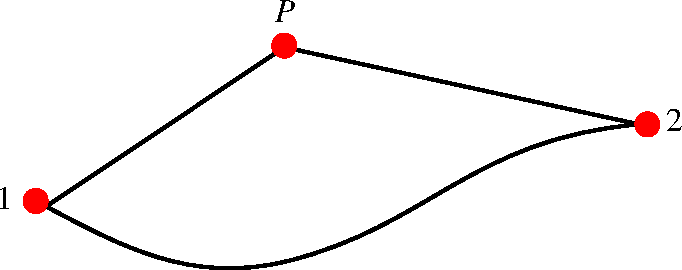
\includegraphics[scale=0.7]{paths}  
\end{minipage}
\begin{minipage}{0.5\linewidth}
  \begin{align}
  \int_1^2 \mathbf{F}\cdot d\mathbf{r}
  =&\int_1^P \mathbf{F}\cdot d\mathbf{r}+\int_P^2 \mathbf{F}\cdot d\mathbf{r}\nonumber\\
  =&-\int_P^1 \mathbf{F}\cdot d\mathbf{r}+\int_P^2 \mathbf{F}\cdot d\mathbf{r}\nonumber\\
  =&-(-U(x_1,y_1,z_1))-U(x_2,y_2,z_2)\nonumber\\
  =&U(x_1,y_1,z_1)-U(x_2,y_2,z_2)\nonumber\\
  =&U(\mathbf{r}_1)-U(\mathbf{r}_2)\,.
\end{align}
\end{minipage}

La cantidad $U(\mathbf{r}_1)-U(\mathbf{r}_2)$ es llamada el cambio en \emph{energía potencial}, y llamaremos $U$ la energía potencial.

Para el caso de fuerzas conservativas, la ec.~(\ref{eq:tte}) queda
\begin{align}
  U(\mathbf{r_a})-U(\mathbf{r_b})=&K_b-K_a\nonumber\\
  K_a+U(\mathbf{r_a})=&K_b+U(\mathbf{r_b})\,,
\end{align}
Como esto se mantiene para cualquier par de puntos $\mathbf{r}_a$ y $\mathbf{r}_b$, entonces
\begin{align}
  E\equiv K+U=\text{constante}\,.
\end{align}
La constante $E$ es llamada la \emph{energía mecánica} de la partícula, o de forma menos precisa, la energía total de la partícula. 

La Ley de Convervación de la Energía Mecánica es una consecuencia de la homogeneidad del tiempo.

Supongamos que tenemos un sistema unidimensional, en el cual la fuerza $F(x)$ es conservativa, de modo que la diferencia de energía potencial es
\begin{align}
  U_b-U_a=&-\int_C \mathbf{F}\cdot d\mathbf{r}\nonumber\\ 
  =&-\int_{t_a}^{t_b} \mathbf{F}\cdot \frac{d\mathbf{r}}{dt}dt\nonumber\\ 
  =&-\int_{t_a}^{t_b} F\frac{dx}{dt}dt\nonumber\\ 
  =&-\int_{x_a}^{x_b} F\,{dx}\,.
\end{align}
Consideremos el cambio en la energía potencial $\Delta U$ a medida que la partícula se mueve desde algún punto $x$ a $x+\Delta x$
\begin{align}
  U(x+\Delta x)-U(x)\equiv&\Delta U\nonumber\\
  =&-\int_x^{x+\Delta x}F(x)\,dx\nonumber\\
\approx &-F(x)\int_x^{x+\Delta x}\,dx\nonumber\\
=&-F(x)(x+\Delta x-x)\nonumber\\
=&-F(x)\Delta x\,,
\end{align}
o
\begin{align}
  F(x)\approx -\frac{\Delta U}{\Delta x}
\end{align}
en el límite $\Delta x\to 0$ estaríamos tentados a escribir $dU/dx$, sin embargo es más conveniente hacer explícito que la variación es sólo sobre $x$ usando la notación
\begin{align}
  F(x)= -\frac{\partial U}{\partial x}
\end{align}
definida como la derivada parcial por los matemáticos. Note entonces que en el caso unidimensional la energía potencial es justamente la antiderivada de $F(x)$

En el caso de una fuerza conservativa en tres dimensiones siempre podemos escoger una trayectoria para ir del punto 1 al punto 2 de tal forma que se mantengan dos de las direcciones constantes. A lo largo de cada dirección podemos aplicar el método anterior variando $U$ sólo en la dirección relevante. Por ejemplo,
para una fuerza en tres dimensiones
\begin{align}
  \mathbf{F}=F_x\hat{\mathbf{i}}+F_y\hat{\mathbf{j}}+F_y\hat{\mathbf{k}}\,,
\end{align}
si escogemos una trayectoria a lo largo de $x$ llegaríamos al resultado
\begin{align}
  F_x=&-\lim_{\Delta x\to 0} \frac{U(x+\Delta x,y,z)}{\Delta x}\nonumber\\
  =&-\left.\frac{\partial U}{\partial x}\right|_{yz}\,.
\end{align}
donde la parte de ``$|_{yz}$'' hace explícito que la variación se hace manteniendo las direcciones $y$ y $z$ constantes. En adelantes usaremos la notación de derivadas parciales sin explicitar la variables que se dejan constantes pues se sobreentiende del contexto.

Por un método completamente análogo para las otras direcciones, se llega al sistema de ecuaciones. 

\begin{align}
  F_x=& -\frac{\partial U}{\partial x}\nonumber\\
   F_y=& -\frac{\partial U}{\partial y}\nonumber\\
   F_z=& -\frac{\partial U}{\partial z}\,.
\end{align}
O en notación vectorial
\begin{align}
 \mathbf{F}=F_x\hat{\mathbf{i}}+F_y\hat{\mathbf{j}}+F_z\hat{\mathbf{k}}
=&-\left(\hat{\mathbf{i}}\frac{\partial U}{\partial x}
+\hat{\mathbf{j}}\frac{\partial U}{\partial y}
+\hat{\mathbf{k}}\frac{\partial U}{\partial z}\right)\nonumber\\
=&-\left(\hat{\mathbf{i}}\frac{\partial }{\partial x}
+\hat{\mathbf{j}}\frac{\partial }{\partial y}
+\hat{\mathbf{k}}\frac{\partial }{\partial z}
\right)U\nonumber\\
\mathbf{F}\equiv& -\boldsymbol{\nabla}U\,.
\end{align}
El operador
\begin{align}
\boldsymbol{\nabla}\equiv \hat{\mathbf{i}}\frac{\partial }{\partial x}
+\hat{\mathbf{j}}\frac{\partial }{\partial y}
+\hat{\mathbf{k}}\frac{\partial }{\partial z}
\end{align}
se llama \emph{gradiente} y convierte una función escalar de varias variables en una función vectorial. De éste modo para un campo conservativo, la integral de línea entre $a$ y $b$ se puede evaluar dando como resultado:
\begin{align}
  \int_C\mathbf{F}\cdot d\mathbf{r}=U(\mathbf{r}_a)-U(\mathbf{r}_b)
\end{align}
Generalizando el caso de la integración normal en una variable,
$-U(\mathbf{r})$ se podría ver como el ``antigradiente'' de
$\mathbf{F}$. El concepto de fuerza conservativa tiene su contraparte
matemática para establecer teoremas de integrabilidad de funciones de
varias variables. Para las fuerzas conservativas el campo generado por
el vector de fuerza se puede conocer a partir del \emph{gradiente} de
variaciones de una función escalar llamada el potencial.

\section{Conservación de la energía}
Las fuerzas fundamentales, o más estrictamente, las interacciones
fundamentes conocidas en la naturaleza, son todas conservativas. Como
consecuencia, la energía total de un sistema de partículas se debe
conservar. Estas interacciones fundamentales pueden generar algunas
fuerzas remanentes como la fricción que aparentemente es no
conservativa: el trabajo para arrastrar un objeto entre un par de
puntos por diferentes caminos con fricción, depende de la trayectoria
que se siga el objeto. Sin embargo, la fricción es una herramienta
para parametrizar detalles de las interacciones interatómicas las
cuales si son conservativas. La energía cinética y los diferentes
potenciales interatómicos cambian con el movimiento de un cuerpo sobre una
superficie con fricción. Estos procesos se reflejan en el calor
disipado por el cuerpo mientras se mueve sobre la superficie. En
términos modernos la temperatura de un material es una consecuencia
de la energía cinética y potencial de sus componentes. Si tenemos en
cuenta la energía mecánica del sistema y las perdidas por calor, la
energía total del sistema se debe conservar, aunque en la practica
resulte extremadamente complicado calcular el calor generado por las
interacciones conservativas entre los átomos y moléculas del sistema.

Como dijimos antes, Joule fue el primer en apreciar que
el calor en si mismo representa una forma de energía. 
En nuestros días tenemos un conocimiento más detallado de la energía
calórica que la que tenía Joule. Sabemos que los sólidos están
compuestos por átomos mantenidos juntos por fuertes interacciones
interatómicas. Cada átomo puede oscilar sobre su posición de
equilibrio y tiene una energía mecánica en forma de energías cinéticas
y potenciales provenientes de interacciones conservativas. A medida
que el sólido se calienta, la amplitud de las oscilaciones se
incrementa y la energía promedio de cada átomo se vuelve mayor. La
energía calórica de un sólido es la energía mecánica de las
vibraciones aleatorias de los átomos.
   

\section{Ejemplos de energía potencial}

\subsection{Energía potencial de un campo de fuerza uniforme}
\begin{align}
  U(h)=mgh\,,
\end{align}
donde $h$ es la altura desde el suelo.

\begin{itemize}
\item[\textbf{Ejemplo:}] \textbf{Caída libre}\\
Si $\mathbf{F}=-mg\hat{\mathbf{j}}$, $d\mathbf{r}=\hat{\mathbf{j}}dy$ tenemos
\begin{align}
\label{eq:12e}
  \tfrac{1}{2}mv_b^2-\tfrac{1}{2}mv_a^2=&\int\mathbf{F}\cdot d\mathbf{r}\nonumber\\
  =&-mg \int_{y_a}^{y_b}\, dy\nonumber\\
  \tfrac{1}{2}mv_b^2-\tfrac{1}{2}mv_a^2=&-gm(y_b-y_a)\,.
\end{align}

De esta forma hemos obtenido directamente la ecuación de la trayectoria para caída libre \eqref{eq:trayl}
\begin{align}
  \tfrac{1}{2}v_b^2-\tfrac{1}{2}v_a^2=&-g(y_b-y_a)\,.
\end{align}

En términos de conservación de la energía mecánica, la ec~(\ref{eq:12e}) también puede escribirse como:
\begin{align}
  \tfrac{1}{2}v_a^2+mgy_a=&\tfrac{1}{2}mv_b^2+mgy_b
\end{align}


Para encontrar la altura máxima de un cuerpo lanzado horizontalmente hacia arriba desde la superficie de la tierra, con rapidez inicial $v_0$, igualamos la energía cinética incial con la energía potencial final:
\begin{align}
  \frac{1}{2}mv_0^2=mgy_{\text{max}}\,,
\end{align}
de donde
\begin{align}
  y_{\text{max}}=\frac{v_0^2}{2g}\,.
\end{align}

\end{itemize}


\ejemplo{}
\label{ex:polea}


 Un cuerpo de masa $m_2$ se desliza desde el
  reposo sobre una mesa sin fricción debido al peso de un bloque de
  masa $m_1>m_2$ que cae desde una altura $y_0$ y con el cual está
  conectado a través de una polea ideal. Ver figura~\ref{fig:poleaideale}

La conservación de energía se aplica al sistema completo:
\begin{align}
  \text{Energía mecánica inicial de los dos bloques}=
\text{Energía mecánica final de los dos bloques}
\end{align}
Como los dos bloques se mueven con la misma rapidez $v$, y asumiendo
sin perdida de generalidad que la altura final del bloque 1 es cero,
tenemos (asumiendo que la altura de la mesa es $h$)

\begin{frame}
  \begin{figure}
    \centering
    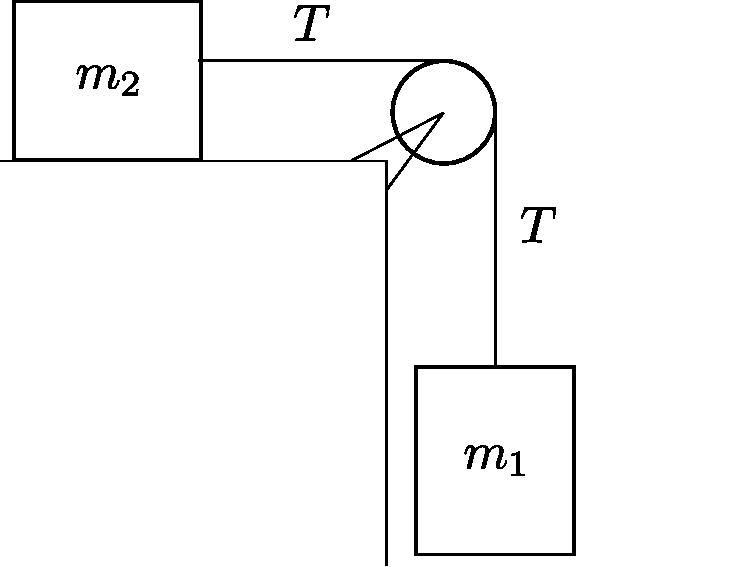
\includegraphics[scale=0.5]{poleaideal}
    \caption{Polea ideal}
    \label{fig:poleaideale}
  \end{figure}
\end{frame}

\begin{frame}
\begin{align*}
  m_1gy_0+\cancel{m_2gh}=&\tfrac{1}{2}m_1 v^2+\tfrac{1}{2}m_2 v^2+\cancel{m_2gh}\phantom{\color{red}+Q}\nonumber\\
 \phantom{\color{red}-\mu m_2 g y_0+}m_1gy_0=&\tfrac{1}{2}m_1 v^2+\tfrac{1}{2}m_2 v^2
  =\tfrac{1}{2}(m_1+m_2) v^2\,,
\end{align*}
despejando $v$, obtenemos
\begin{align*}
  v^2=2gy_0\,\frac{m_1\phantom{\color{red}-\mu m_2}}{m_1+m_2}\,.
\end{align*}
Para un movimiento bajo aceleración constante, y teniendo en cuenta que la altura final es cero
\begin{align*}
  0=&y_0-\tfrac{1}{2}a\Delta t^2\,,&
  v=&-a\Delta t\,,
\end{align*}
tenemos, de la última ecuación
\begin{align*}
  a^2 \Delta t^2=v^2
  =&2gy_0\,\frac{m_1\phantom{\color{red}-\mu m_2}}{m_1+m_2}\nonumber\\
  a^{\cancel{2}} \cancel{\Delta t^2}=&\frac{2}{2}g\,\cancel{a\Delta t^2}\,\frac{m_1\phantom{\color{red}-\mu m_2}}{m_1+m_2}\,,
\end{align*}
de donde
\begin{align}
\label{eq:acelfin}
  a=g\,\frac{m_1\phantom{\color{red}-\mu m_2}}{m_1+m_2}\,,
\end{align}
\end{frame}
que coincide con el resultado expresado en la ecuación \eqref{eq:polea} cuando $\mu=0$.


Usando directamente las leyes de Newton, como hicimos en los problemas resueltos del capítulo de dinámica
\begin{align}
  T=&m_2 a\nonumber\\
m_1g-T=&m_1 a\,,
\end{align}
donde $T$ es la tensión de la cuerda. 


\begin{inprogress}
  \begin{itemize}
  \item[\textbf{Ejemplo:}] \textbf{Energía potencial de un campo de fuerza uniforme}
  \end{itemize}
\end{inprogress}

\begin{inprogress}
  \begin{itemize}
  \item[\textbf{Ejemplo:}] \textbf{El péndulo invertido}
  \end{itemize}
\end{inprogress}


\section{Fuerzas no conservativas}
La fuerza total se puede escribir como
\begin{align}
  \mathbf{F}=\mathbf{F}^{\text{c}}+\mathbf{F}^{\text{nc}}
\end{align}
donde $\mathbf{F}^{\text{c}}$ y $\mathbf{F}^{\text{nc}}$ son las fuerzas conservativas y no conservativas respectivamente. El trabajo total es
\begin{align}
  W_{ba}^{\text{total}}=&\int_C \mathbf{F}\cdot d\mathbf{r}\nonumber\\
=&\int_C \mathbf{F}^{\text{c}}\cdot d\mathbf{r}+\int_C \mathbf{F}^{\text{nc}}\cdot d\mathbf{r}\nonumber\\
=-U_b+U_a+W_{ba}^{\text{nc}}\,.
\end{align}
Aquí $U$ es la energía potencial asociada con las fuerza conservativa y $W_{ab}^{\text{nc}}$ es el trabajo hecho por la fuerza no conservativa. El teorema de trabajo-energía, $W_{ba}^{\text{total}}=K_b-K_a$, ahora toma la forma
\begin{align}
  -U_b+U_a+W_{ba}^{\text{nc}}=K_b-K_a\,,
\end{align}
ó
\begin{align}
  K_b+U_b=K_a+U_a+W_{ba}^{\text{nc}}\,.
\end{align}
Si definimos la energía mecánica por
\begin{align}
  E=K+U\,,
\end{align}
tenemos
\begin{align}
  E_b-E_a=W_{ba}^{\text{nc}}\,.
\end{align}

Si definimos $Q=-W_{ab}$ como la energía disipada: la diferencia entre
la energía mecánica inicial y final
\begin{align}
  E_a=&E_b-W_{ba}^{\text{nc}}\nonumber\\
   E_a=&E_b+Q.
\end{align}
En el caso por ejemplo de la un movimiento en presencia de una fuerza
no conservativa como la fricción, $Q$ corresponde a la energía
disipada en forma de calor.

En el caso del ejemplo asociado a la figura~\ref{fig:poleaideale}, si consideramos que entre las dos superficies hay fuerza fricción, esta realiza un trabajo sobre el bloque $m_2$ que se disipa en calor $Q$, a medida que el cuerpo de masa $m_1$ cae una distancia $y_0$. El calor disipado esta dado por
\begin{align*}
    {\color{red}Q}=-W_{ba}=&\int_C \mathbf{F}\cdot d\mathbf{r}\nonumber\\
=&\int_C
\begin{pmatrix}
  -\mu m_2g,&0,&0
\end{pmatrix}\cdot
\begin{pmatrix}
dx,&dy,&dz  
\end{pmatrix}\nonumber\\
=&-(-\mu m_2 g)\int_0^{y_0}dx\nonumber\\
&={\color{red}\mu m_2g y_0\,,}
\end{align*}
donde $\mu$, es el coeficiente de fricción y donde hemos usado la
ligadura consistente en que la distancia vertical recorrida es la
misma que la distancia horizontal, pues la cuerda es ideal.
Repitiendo los pasos que dieron lugar a la ec.~\eqref{eq:acelfin}


\begin{frame}
\begin{align*}
  m_1gy_0+\cancel{m_2gh}=&\tfrac{1}{2}m_1 v^2+\tfrac{1}{2}m_2 v^2+\cancel{m_2gh}{\color{red}+Q}\nonumber\\
 {\color{red}-\mu m_2 g y_0+}m_1gy_0=&\tfrac{1}{2}m_1 v^2+\tfrac{1}{2}m_2 v^2
  =\tfrac{1}{2}(m_1+m_2) v^2\,,
\end{align*}
despejando $v$, obtenemos
\begin{align*}
  v^2=2gy_0\,\frac{m_1{\color{red}-\mu m_2}}{m_1+m_2}\,.
\end{align*}
Para un movimiento bajo aceleración constante, y teniendo en cuenta que la altura final es cero
\begin{align*}
  0=&y_0-\tfrac{1}{2}a\Delta t^2\,,&
  v=&-a\Delta t\,,
\end{align*}
tenemos, de la última ecuación
\begin{align*}
  a^2 \Delta t^2=v^2
  =&2gy_0\,\frac{m_1{\color{red}-\mu m_2}}{m_1+m_2}\nonumber\\
  a^{\cancel{2}} \cancel{\Delta t^2}=&\frac{2}{2}g\,\cancel{a\Delta t^2}\,\frac{m_1{\color{red}-\mu m_2}}{m_1+m_2}\,,
\end{align*}
de donde
\begin{align}
\label{eq:acelfinmu}
  a=g\,\frac{m_1{\color{red}-\mu m_2}}{m_1+m_2}
\end{align}

\end{frame}

\noindent
que coincide exactamente con el resultado obtenido en la ecuación \eqref{eq:polea} utilizando las ecuaciones de la dinámica. 

\begin{frame}
  \begin{block}{Recomendación}
    \emph{Siempre que pueda, resuelva los problemas por dos métodos diferentes y compruebe que obtiene la misma respuesta!}
    \begin{center}
          \begin{tabular}{cc}
      Ecuaciones de movimiento & Teorema trabajo y energía\\
      $\displaystyle a=g\,\frac{m_1{\color{red}-\mu m_2}}{m_1+m_2}$&
      $\displaystyle a=g\,\frac{m_1{\color{red}-\mu m_2}}{m_1+m_2}$\\
    \end{tabular}
    \end{center}
  \end{block}
\end{frame}

\begin{inprogress}
  \begin{itemize}
  \item[\textbf{Ejemplo:}] \textbf{Bloque deslizándose por un plano
      inclinado (Ejemplo 4.17 de Klepner)}\\
  \end{itemize}
\end{inprogress}


\section{Energía potencial de un resorte}
Por sencillez consideremos el caso de un resorte que se mueve a lo largo del eje $x$, como se muestra en la figura~\ref{fig:resorte}. Para una elongación $x-x_0$ a partir de su posición de equilibrio $x_0$ la fuerza está dada por la Ley de Hooke
\begin{align}
  \mathbf{F}=-k(x-x_0)\hat{\mathbf{i}}\,.
\end{align}
\begin{frame}
  \begin{figure}
    \centering
%\only<1>%
{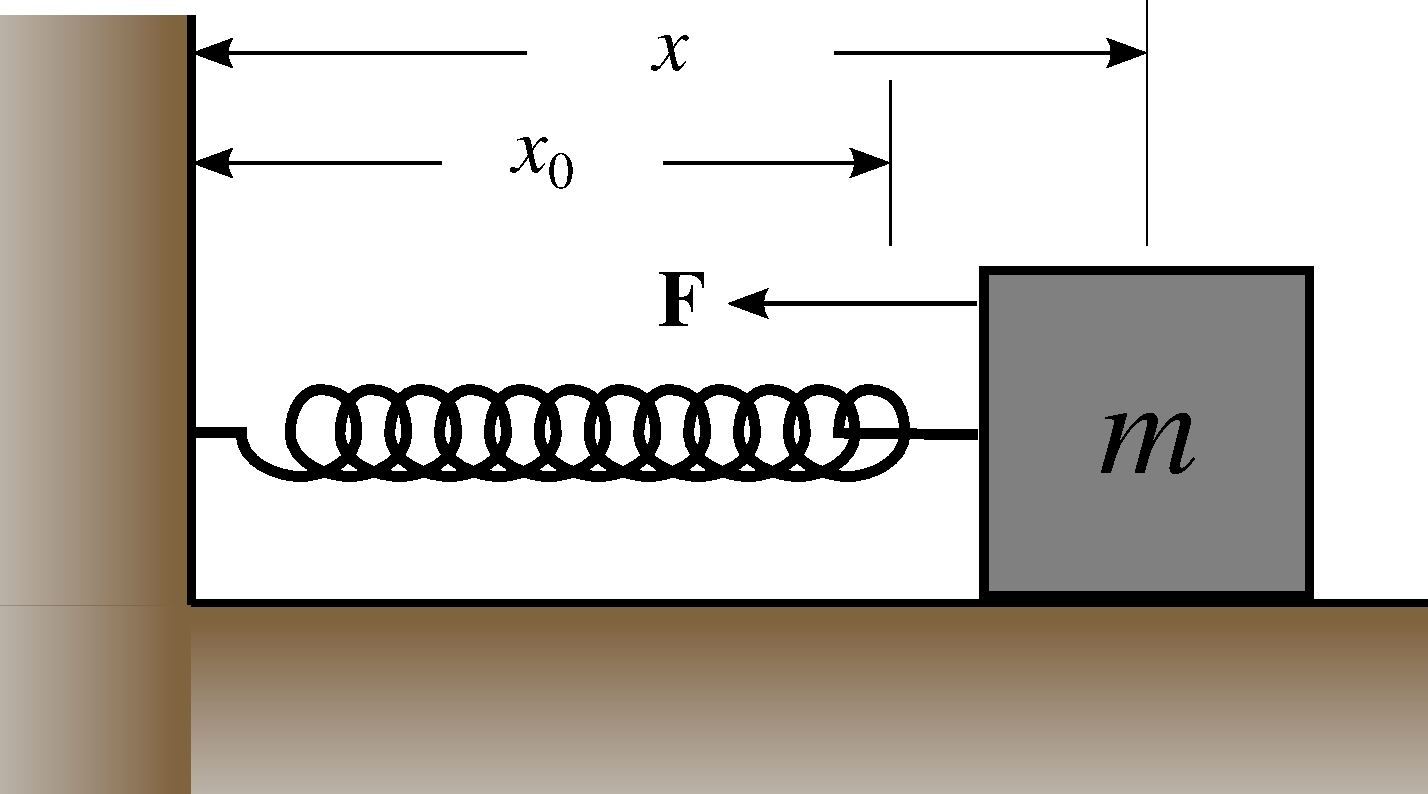
\includegraphics[scale=0.5]{resorte1}}
%\only<2>{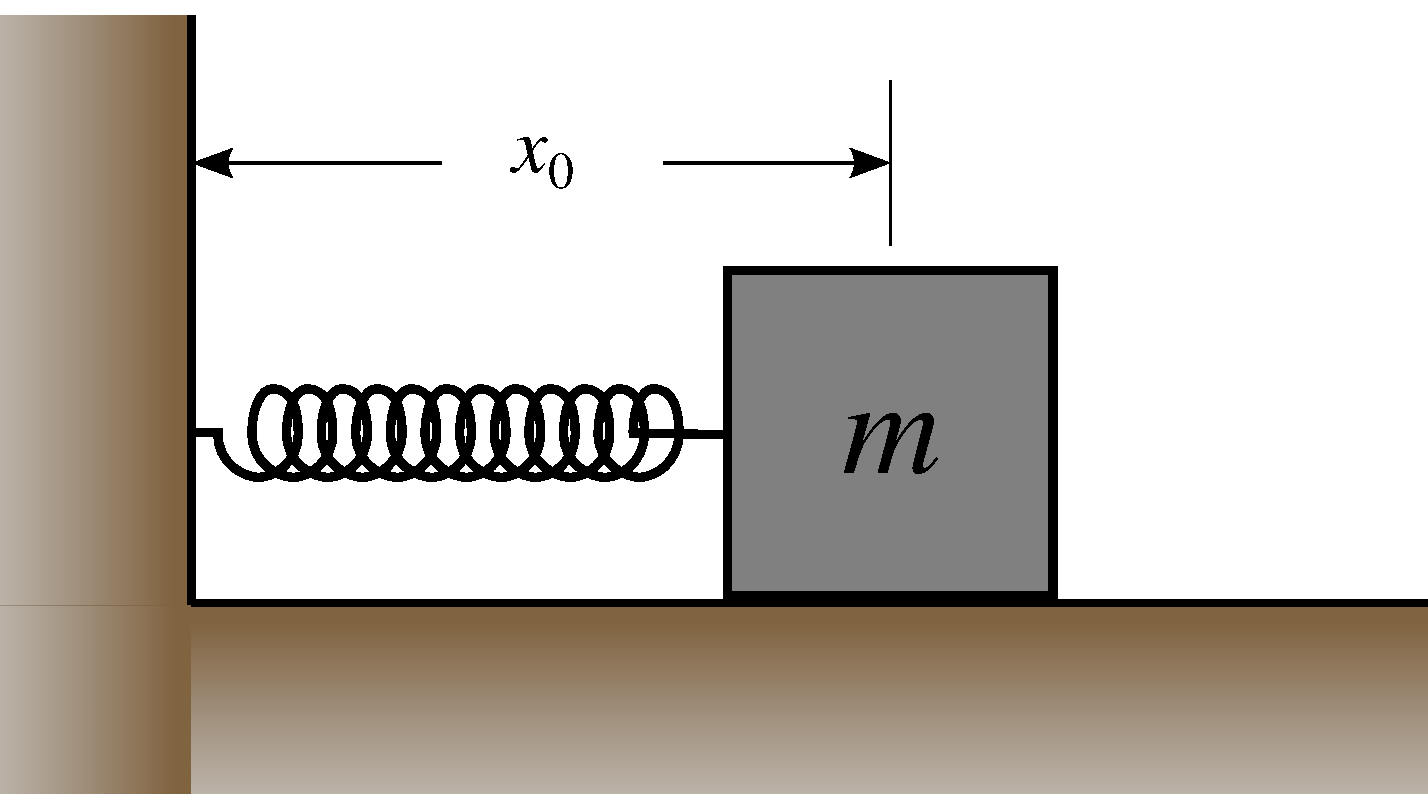
\includegraphics[scale=0.5]{resorte2}}%
%\only<3>{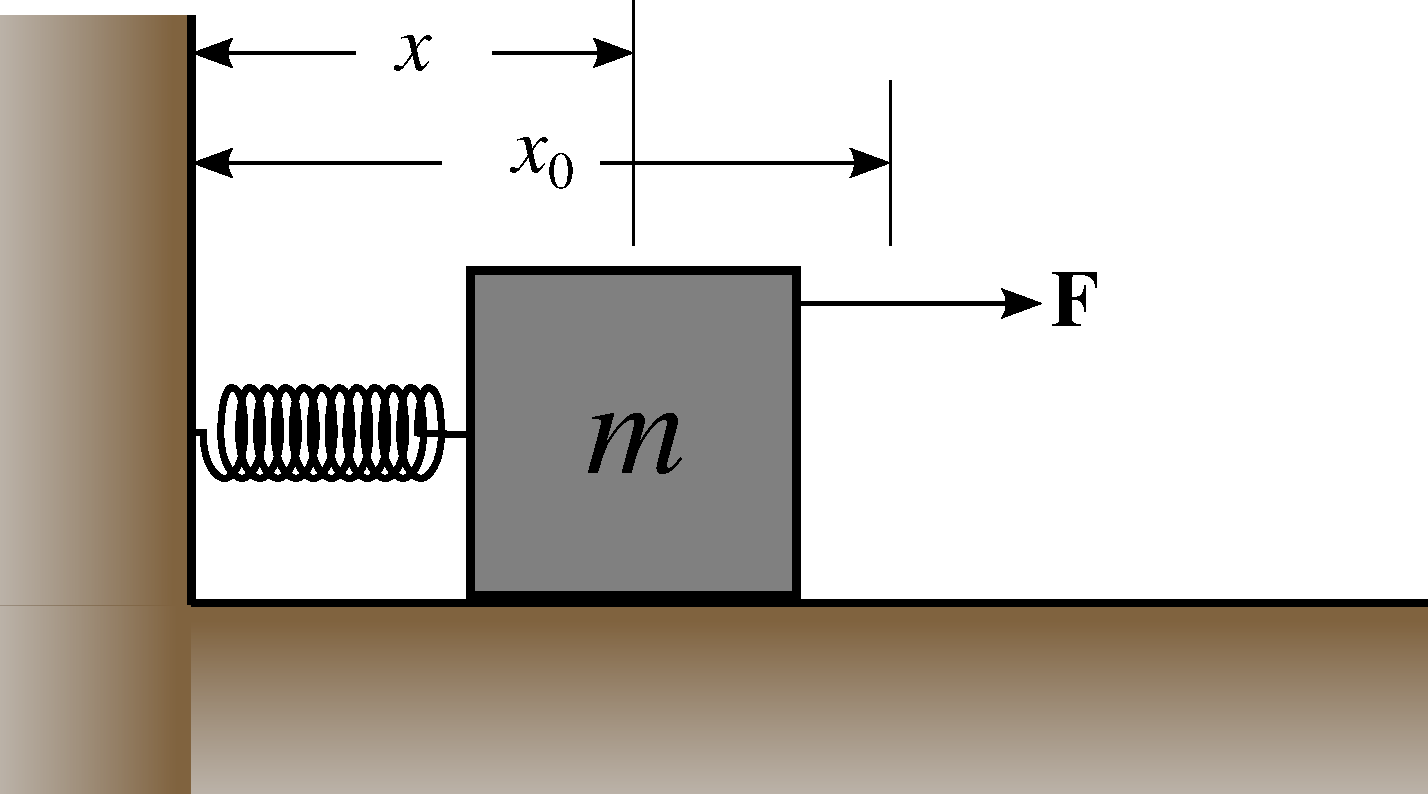
\includegraphics[scale=0.5]{resorte3}}%
    \caption{Resorte (Adaptado de Wikipedia)}
    \label{fig:resorte}
  \end{figure}
\end{frame}

El trabajo para ir de $a$ a $b$ es
\begin{align}
  W_{ab}=&\int \mathbf{F}\cdot d\mathbf{r}\nonumber\\
  =&\int_{x_a}^{x_b} Fdx\nonumber\\
  =&-k\int_{x_a}^{x_b} (x-x_0)dx\nonumber\\
  =&-\tfrac{1}{2}k \left.
    (x-x_0)^2\right|_{x_0}^x\nonumber\\
  =&-\tfrac{1}{2}k (x-x_0)^2+0\nonumber\\
  =&+0+C-(\tfrac{1}{2}k (x-x_0)^2+C)\nonumber\\
  =&U(x_0)-U(x)\,.
\end{align}
Y viceversa: de la siguiente energía potencial para el resorte,
\begin{align}
  U(x)=&\tfrac{1}{2}k{(x-x_0)^2}+C& C=&\text{contante}\,,
\end{align}
se puede obtener la fuerza conservativa
\begin{align}
  \mathbf{F}=-\frac{\partial}{\partial x}U(x)\hat{\mathbf{i}}
=&\left(
-\frac{2}{2}k(x-x_0)\frac{\partial}{\partial x}(x-x_0)+0
\right)\hat{\mathbf{i}}\nonumber\\
=&-k(x-x_0)\hat{\mathbf{i}}\,.
\end{align}

Por convención escogemos que la energía potencial sea cero en la posición de equilibrio:
\begin{align}
  U(x_0)=0=&\tfrac{1}{2}k{(x_0-x_0)^2}+C\nonumber\\
  0=&C\,,
\end{align}
de modo que la energía potencial para el resorte es
\begin{align}
  U(x)=&\tfrac{1}{2}k{(x-x_0)^2}\,.
\end{align}

\ejemplo{}
\label{ex:resorte}

En $t=0$ una masa atada a un resorte sobre
una superficie horizontal sin fricción, es
liberada desde el reposo a una distancia $x_i$ desde la posición de
equilibrio de un resorte. Encuentre la posición de la masa en
  cualquier tiempo posterior. Asumamos sin perdida de generalidad que
  la posición de equilibrio del resorte se encuentra en $x_0=0$

Usando la conservación de la Energía Mecánica:
\begin{align}
  K_i+U_i=&K_f+U_f\nonumber\\
 \tfrac{1}{2}kx_i^2=&\tfrac{1}{2}m v^2+\tfrac{1}{2}kx^2\nonumber\\
 kx_i^2=&m v^2+kx^2\,,
\end{align}
despejando $v$:
\begin{align}
  v=\sqrt{\frac{k}{m}}\sqrt{x_i^2-x^2}
\end{align}
note que la conservación de energía implica que $x\le x_i$. Entonces
\begin{align}
  \frac{dx}{dt}=\sqrt{\frac{k}{m}}\sqrt{x_i^2-x^2}\,.
\end{align}
Reorganizando términos
\begin{align}
  \label{eq:intosc}
  \frac{dx}{\sqrt{x_i^2-x^2}}=\omega dt\,,
\end{align}
donde hemos definido la frecuencia angular $\omega$ como:
\begin{align}
  \omega\equiv \sqrt{\frac{k}{m}}\,.
\end{align}
Integrando \eqref{eq:intosc}
\begin{align}
  \label{eq:intosc}
  \int_{x_i}^x\frac{dx}{\sqrt{x_i^2-x^2}}=\omega\int_0^t dt\,,
\end{align}
\begin{align}
\left.\sin^{-1}\left(\frac{x}{x_i}  \right)\right|_{x_i}^x=&\omega t\nonumber\\
\sin^{-1}\left(\frac{x}{x_i} \right)-\sin^{-1}\left(1\right)=&\omega t\nonumber\\
\sin^{-1}\left(\frac{x}{x_i} \right)-\frac{\pi}{2}=&\omega t\,,
\end{align}
despejando $x$, tenemos
\begin{align}
  x=x_i\sin\left(\omega t +\frac{\pi}{2}\right)
\end{align}
o
\begin{align}
  x=x_i\cos(\omega t)
\end{align}

  
%\left(  \right)


\begin{inprogress}
  \subsection{Estabilidad}

\section{Diagramas de energía}

\section{Oscilaciones pequeñas en un sistema ligado}

\end{inprogress}


  
\section{Potencia}
Potencia es la tasa de cambio del trabajo realizado. Si una fuerza $\mathbf{F}$ actúa en un cuerpo que sufre un desplazamiento $\Delta\mathbf{r}$, tenemos que el trabajo en dicho segmento es de la ec.\eqref{eq:dW}
\begin{align}
  \Delta W_j=\mathbf{F}(\mathbf{r}_j)\cdot \Delta \mathbf{r}_j\,.
\end{align}
en el límite $\Delta t\to 0$
\begin{align}
  dW=\mathbf{F}\cdot d\mathbf{r}\,.
\end{align}
Definimos la potencia desarrollada por la fuerza como
\begin{align}
  P=\frac{dW}{dt}=&\mathbf{F}\cdot \frac{d\mathbf{r}}{dt}\nonumber\\
=&\mathbf{F}\cdot \mathbf{v}\,.
\end{align}
La unidad de potencia en el sistema SI es el watt (W):
\begin{align}
  \SI{1}{\watt}=\SI{1}{\joule\per\second}\,.
\end{align}
La relación entre un caballo de fuerza y el watt es
\begin{align}
  1\;\text{hp}\approx \SI{746}{\watt}\,.
\end{align}
\example{} 
En la factura eléctrica se cobra la energía consumida al
mes.  El joule es una unidad demasiado pequeña, lo que obligaría a
emplear cifras demasiado grandes, por eso es conveniente reescribirlo
en potencia mayores. Note que
\begin{align}
  \SI{1}{\joule}=\si{\watt\second}\,.
\end{align}
De acuerdo a esto, pase a Joules las siguientes cantidades de energía
\begin{enumerate}
\item El $\si{\kilo\watt\hour}$ usado para medir el consumo electríco.
\item Los $\SI{75}{\giga\watt\hour}$ que consume el metro de Medellín en un año. 
%Si toda esa energía se pudiese convertir en energía cinética 
\end{enumerate}
\begin{align*}
  \SI{1}{\kilo\watt\hour}=&\SI{1000}{\watt}\cdot \SI{3600}{\second}\nonumber\\
  =&1000\frac{\si{\joule}}{\si{\second}}\cdot \SI{3600}{\second}\nonumber\\
  =&\SI{3600000}{\joule} \,.
\end{align*}

\begin{align*}
  \SI{75}{\giga\watt\hour}=&75\times 10^9\si{\watt}\cdot \SI{3600}{\second}\nonumber\\
  =&2.7\times 10^{14}\si{\joule}\,.
\end{align*}



\section{Colisiones}
Un sistema de dos partículas interaccionando en ausencia de fuerzas externas conserva el momentum total, de modo que
\begin{align}
\label{eq:consmom}
  \mathbf{P}_i=&\mathbf{P}_f\nonumber\\
m_1\mathbf{v}_1+m_2\mathbf{v}_2=&m_1\mathbf{v}'_1+m_2\mathbf{v}'_2\,.
\end{align}


\subsection{Colisiones elásticas}
Una colisión en la cual la energía la energía cinética no cambia 
es llamada una \emph{colisión elástica}. Una colisión es elástica si
las fuerzas de interacción son conservativas, como por ejemplo la
interacción entre dos bloques que se deslizan sin fricción
interaccionando a través de resortes, como se ilustra en la
figura~\ref{fig:colisionelastica}.


\begin{frame}
En tal caso, la conservación de la energía cinética da lugar a la ecuación
\begin{equation}
\label{eq:E2}
  m_1 v^2_1 + m_2 v^2_2 = m_1 {v'}^2_1 + m_2 {v'}^2_2\,.
\end{equation}

Si la colisión se desarrolla en una sola dimensión, la ec.~\eqref{eq:consmom} se reduce a 
\begin{equation}\label{eq:E1}
  m_1 v_1 + m_2 v_2 = m_1 v_1' + m_2 v_2'\,,
\end{equation}

Tenemos entonces un sistema de dos ecuaciones que podemos resolver
para las dos incógnitas $v_1'$ y $v_2'$. La solución es
\begin{align}
  v_1' =& \frac{(m_1 - m_2)v_1 + 2m_2 v_2}{m_1 + m_2} \nonumber\\
  v_2' =& \frac{(m_2 - m_1)v_2 + 2m_1 v_1}{m_1+ m_2}
\end{align}
\end{frame}


\ejemplo{}
\textbf{Colisiones entre dos bloques:}\footnote{Elaborado por Alexander Gallego}\\
Considere la colisión entre dos bloques que interactúan a través de un
resorte, como se muestra en la
figura~\ref{fig:colisionelastica}. 
Antes de la colisión el bloque de masa $m_1$ se mueve hacia la derecha
con rapidez $u_1$ y el bloque de masa $m_2$ se encuentra en
reposo. 
Encuentre las velocidades finales $v_1$ y $v_2$ en función de $u_1$ y
las masas.

\begin{figure}
  \centering
  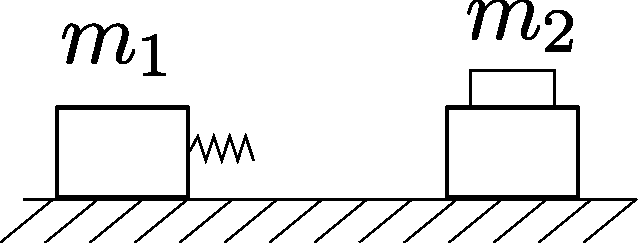
\includegraphics{colisionelastica}
  \caption{Colisión elástica}
  \label{fig:colisionelastica}
\end{figure}

Como la colisión ocurre prácticamente en un punto, podemos despreciar
la energía disipada en calor durante el pequeño intervalo de tiempo
que dura la colisión. Entonces la energía cinética se conserva antes y
después de la colisión. 

Conservación de moméntum
\begin{align}
  \label{eq:e1}
  p_{i}=&p_f\nonumber\\
  m_1 u_1 =& m_1 v_1 + m_2 v_2\,.
\end{align}

Conservación de energía cinética
\begin{align}
  \label{eq:e2}
  K_i=&K_f\nonumber\\
  m_1 u^2_1 =& m_1 v^2_1 + m_2 v^2_2\,.
\end{align}

De (\ref{eq:e1})
\begin{equation}
  \label{eq:v1}
  v_1 = \frac{1}{m_1}( m_1u_1 - m_2 v_2),
\end{equation}
Reemplazando $v_1$ en \ref{eq:e2}
\begin{equation}
   m_1 u_1^2 = m_1 \left( \frac{m_1u_1 - m_2 v_2}{m_1} \right)^2 +  m_2 v^2_2\,,
\end{equation}
y desarrollando el binomio
\begin{align}
 m_1 u_1^2 =& \frac{1}{m_1}( m_1^2 u_1^2 - 2 m_1 m_2 u_1 v_2 + m_2^2 v_2^2) + m_2 v_2^2\nonumber\\
m_1 u_1^2 =&  m_1 u_1^2 - 2 m_2 u_1 v_2 + \frac{m_2^2}{m_1} v_2^2 + m_2 v_2^2\,.
\end{align}
Cancelando $m_1 u_1^2$ a ambos lados y dividiendo por $m_2v_2$ y factorizando $v_2$
\begin{align}
  0=& - 2 m_2 u_1 v_2 + \frac{m_2^2}{m_1} v_2^2 + m_2 v_2^2\nonumber\\
  0=& - 2  u_1  + \frac{m_2}{m_1} v_2 + v_2\nonumber\\
  0=& - 2  u_1  + \left(\frac{m_2}{m_1} +1 \right)v_2\nonumber\\
  0=& - 2  u_1  + \left(\frac{m_2+m_1}{m_1}\right)v_2\,,
\end{align}
obtenemos
\begin{equation}
  v_2 = \frac{2m_1}{m_1+ m_2}u_1\,.
\end{equation}
Reemplazando este valor en \eqref{eq:v1}

\begin{align}
  v_1 =& \frac{1}{m_1}\left(m_1u_1 - \frac{2m_2 m_1u_1}{m_1+m_2} \right)\nonumber\\
  =& \frac{u_1}{m_1}\left(m_1 - \frac{2m_2 m_1}{m_1+m_2} \right)\nonumber\\
  =& u_1\left(1 - \frac{2m_2}{m_1+m_2} \right)\nonumber\\
  =& u_1\left(\frac{m_1+m_2 - 2m_2}{m_1+m_2} \right)\nonumber\\
  v_1 = &\frac{m_1 - m_2}{m_1 + m_2} u_1
\end{align}
Asumiendo que el bloque 1 se mueve inicialmente hacia la derecha: $u_1>0$,  tenemos los siguientes casos:
\begin{align}
  v_1\to
  \begin{cases}
    =0 & \text{si\ }m_1=m_2\\
    >0 & \text{si\ }m_1>m_2\\
    <0 & \text{si\ }m_1<m_2
  \end{cases}\,.
\end{align}
\finejemplo







\subsection{Colisiones inelásticas}
En un segundo experimento, tome el mismo par de bloques y reemplace el
resorte por una masilla adhesiva. Considere el segundo bloque
inicialmente en reposo. Después de la colisión ambos bloques se quedan
pegados y se mueven con alguna velocidad $v'$. Por conservación del
moméntum
\begin{align}
  m_1 v=(m_1+m_2)v'\,,
\end{align}
de modo que
\begin{align}
  v'=\frac{m_1}{m_1+m_2}v\,.
\end{align}
La diferencia de energías cinéticas inicial menos final:
\begin{align}
  \tfrac{1}{2}m_1v^2-\tfrac{1}{2}(m_1+m_2)v'^2=&
  \tfrac{1}{2}m_1v^2-\tfrac{1}{2}(m_1+m_2)\frac{m_1^2}{(m_1+m_2)^2}v^2\nonumber\\
  =&\tfrac{1}{2}m_1v^2-\tfrac{1}{2}\frac{m_1^2}{m_1+m_2}v^2\nonumber\\
  =&\tfrac{1}{2}m_1v^2  \left(1-\frac{m_1}{m_1+m_2} \right)
\end{align}
es claramente diferente de cero. Por ejemplo, si $m_1=m_2$, la energía
disipada corresponde a la mitad de la energía cinética inicial. La
energía cinética a cambiado debido a que las fuerzas fueron no
conservativas. Parte de la energía del movimiento colectivo fue
transformada en una energía calórica en el proceso de pegado durante
la colisión. Una colisión en la cual la energía es no conservada es
llamada una \emph{colisión inelástica}. Si los cuerpos quedan juntos
después de la colisión, decimos que la colisión es completamente
inelástica.


Aunque la energía total del sistema es siempre conservada en colisiones, parte de la energía cinética puede ser convertida a alguna otra forma. Para tener en cuenta éste hecho, escribamos la conservación de la energía para colisiones como
\begin{align}
\label{eq:calor}
  K_i=K_f+Q\,,
\end{align}
donde $Q=K_i-K_f$ es la cantidad de energía cinética convertida a otra forma

Para colisiones en una dimensión, la ec.~\eqref{eq:consmom}
Conservación de moméntum  se reduce a
\begin{equation}\label{eq:E1}
  m_1 v_1 + m_2 v_2 = m_1 v_1' + m_2 v_2'\,,
\end{equation}
y conservación de energía cinética es
\begin{equation}\label{eq:E2}
  m_1 v^2_1 + m_2 v^2_2 = m_1 {v'}^2_1 + m_2 {v'}^2_2+Q\,.
\end{equation}
Una vez se calcule $Q$, el sistema de dos ecuaciones con dos
incógnitas se puede resolver

\ejemplo{}
\begin{frame}[fragile,allowframebreaks]
 \textbf{Colisiones
    inelásticas:}\footnote{Elaborado por Nicolás Moure} Un bloque de masa $m$ inicialmente en reposo
  en el punto $A$, se deja caer por una superficie circular de radio
  $R$ como se muestra en la figura ~\ref{fig:colision}. Al llegar al
  punto $B$, sufre una colisión totalmente inelástica con un segundo
  bloque de la misma masa y se quedan pegados hasta alcanzar el reposo
  en $D$. Las dos secciones circulares, tramos $AB$ y $CD$, son
  completamente lisas. El tramo $BC$ es rugoso y el coeficiente de
  fricción entre los bloques y la superficie del piso es
  $\mu$. Encuentre el  el ángulo $\theta$ mostrado en la figura ~\ref{fig:colision}

  \begin{figure}
    \centering
    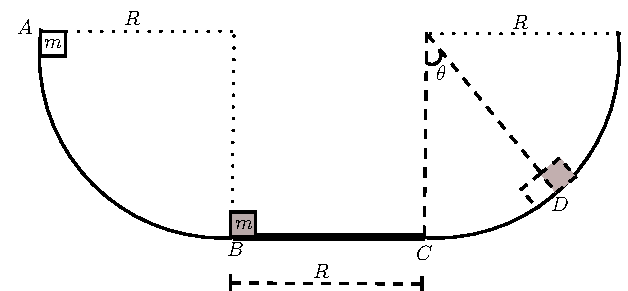
\includegraphics{colision}
    \caption{Ejemplo conservación de energía y colisiones inelásticas}
    \label{fig:colision}
  \end{figure}


\end{frame}

\noindent
\textbf{Solución}] 
En los tramos $AB$ y $CD$ sólo realiza trabajo el peso porque
$\mathbf{N}$ es perpendicular a la trayectoria. En el sector $BC$ sólo
realiza trabajo la fricción, porque el peso y la normal sor
perpendiculares a la trayectoria. El peso es una fuerza conservativa,
mientras que la fricción es una fuerza no conservativa.



En el sector AB: Conservación de la energía
\begin{align}
  mgR=\tfrac{1}{2}m v^2_B\,
\end{align}
de donde
\begin{align}
  v_B=\sqrt{2gR}
\end{align}

En el sector $BC$: El moméntum en la dirección horizontal es igual justo
antes y justo después de la colisión; como la colisión es
completamente inelástica los cuerpos se quedan pegados
\begin{align}
  m v_B=&(m+m) v_B'\nonumber\\
  m v_B=&2m v_B'\nonumber\\
   v_B=&2v_B'\,,
\end{align}
entonces
\begin{align}
  v_B'=&\tfrac{1}{2}v_B\nonumber\\
  =&\tfrac{1}{2}\sqrt{2gR}\nonumber\\
  =&\sqrt{\frac{gR}{2}}\,.
\end{align}
Como la fricción es constante en $BC$,
\begin{align}
  W_f=-f(x_C-x_B)=-f R\,.
\end{align}
Por otro lado $f=\mu N_2=2 m g$, de modo que
\begin{align}
  W_f=-2 \mu m g R=-Q\,.
\end{align}
De la ec.~\eqref{eq:calor}
\begin{align}
  K_B-K_C=Q=2\mu m g R\,.
\end{align}
de donde
\begin{align}
  \tfrac{1}{2}(2m){v_B'}^2-  \tfrac{1}{2}(2m)v_C^2=&2\mu m g R\nonumber\\
  {v_B'}^2- v_C^2=&2\mu  g R
\end{align}
despejando $v_C$
\begin{align}
   v_C^2=&{v_B'}^2-2\mu g R\nonumber\\
\end{align}
\begin{align}
  v_C^2=&\frac{gR}{2}-2\mu g R\nonumber\\
  =&\frac{gR}{2}\left(1-4\mu \right)\,.
\end{align}
de modo que
\begin{align}
  v_C=&\sqrt{\frac{gR}{2}\left(1-4\mu \right)}\,.
\end{align}
El sistema alcanza a llegar a $C$ si $v_c$ es real, esto es si
\begin{align}
  1-4\mu\ge 0\Longrightarrow \mu\le \frac{1}{4}\,.
\end{align}

En el sector CD: Conservación de la energía
\begin{align}
  \tfrac{1}{2}(2m)v_C^2=&2mgh\nonumber\\
&=2mg(R-R\cos\theta)\nonumber\\
&=2mgR(1-\cos\theta)\nonumber\\
  \frac{1}{2}\cdot\frac{gR}{2}\left(1-4\mu \right)&=gR(1-\cos\theta)\nonumber\\
  \frac{1}{4}\left(1-4\mu \right)&=1-\cos\theta\nonumber\\
  \frac{1}{4}-\mu&=1-\cos\theta\,.
\end{align}
\begin{align}
  \cos\theta=&1-\frac{1}{4}+\mu\nonumber\\
  =&\frac{3}{4}+\mu\,,
\end{align}
El $\theta_{\text{min}}$ se obtiene cuando $\mu=1/4$:
\begin{align}
 \cos \theta_{\text{min}}=&1 &\text{o} \qquad \theta_{\text{min}}=0
\end{align}
Así mismo, el $\theta_{\text{max}}$ se obtiene cuando $\mu=0$:
\begin{align}
  \theta_{\text{max}}&\approx 0.723\ \text{rad}\nonumber\\
&\approx 41.4^\circ\,.
\end{align}
Note que si $m=\SI{1}{\kilo\gram}$ y $R=\SI{1}{\meter}$, la energía disipada en
forma de calor en el tramo $BC$ cuando $\mu=0.1$ es
\begin{align}
  Q=&2 \mu m g R\nonumber\\
  =&2\cdot 0.1\cdot \SI{1}{\kilo\gram}\cdot \SI{9.8}{\meter\per\second^2}\cdot
  \SI{1}{\meter}\nonumber\\
  =&\SI{1.96}{\kilo\gram \meter^2\per\second^2}\nonumber\\
  =&\SI{1.96}{\joule}\,.
\end{align}

\finejemplo





\section{Colisiones y coordenadas de centro de masa}
Para estudiar las colisiones de dos partículas que se mueven con
velocidades $\mathbf{v}_1$ y $\mathbf{v}_2$ en lo que se denomina \emph{sistema de
  laboratorio} $L$, es conveniente reescribir las posiciones y velocidades
en el sistema de centro de masa $C$.

Del Capítulo \ref{cha:momentum} sobre moméntum, tenemos:
  \begin{align}
    \label{eq:mbaton}
    \mathbf{R}=\frac{m_1\mathbf{r}_1+m_2\mathbf{r}_2}{m_1+m_2}
  \end{align}
De modo que las coordenadas en el sistema $C$ satisfacen:
\begin{align}
  \mathbf{r}_{1c} =&\mathbf{r}_1-\mathbf{R}\nonumber\\
  \mathbf{r}_{2c}=&\mathbf{r}_2-\mathbf{R}\,.
\end{align}
De la ec.~(\ref{eq:mbaton})
\begin{align}
  \mathbf{r}_{1c}
    =&\frac{m_2}{m_1+m_2}(\mathbf{r}_1-\mathbf{r}_2)\nonumber\\
 \mathbf{r}_{2c}=&-\left(\frac{m_1}{m_1+m_2} \right)\left(\mathbf{r}_1-\mathbf{r}_2 \right)\,.
\end{align}
Derivando con respecto al tiempo estas expresiones, obtenemos
 
\begin{minipage}{0.5\linewidth}
  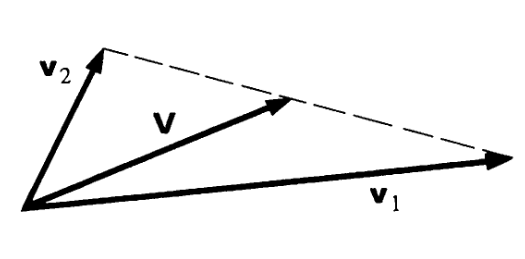
\includegraphics[scale=0.35]{vcm}

\noindent
$V$ está en la línea que une $\mathbf{v}_1$ con $\mathbf{v}_1$.
\end{minipage}
\begin{minipage}{0.5\linewidth}
  \begin{align}
    \label{eq:mbaton}
    \mathbf{V}=\frac{m_1\mathbf{v}_1+m_2\mathbf{v}_2}{m_1+m_2}
  \end{align}
\end{minipage}


\begin{minipage}{0.5\linewidth}
  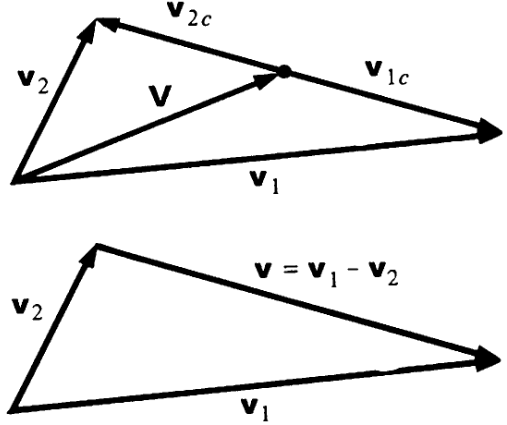
\includegraphics[scale=0.35]{v12cm}

\noindent
$\mathbf{v}_{1c}$ y $\mathbf{v}_{2c}$ están en direcciones opuestas a lo largo del vector de velocidad relativa $\mathbf{v}=\mathbf{v}_1-\mathbf{v}_2$
\end{minipage}
\begin{minipage}{0.5\linewidth}
De modo que las coordenadas en el sistema $C$ satisfacen:
\begin{align}
  \mathbf{v}_{1c} =&\mathbf{v}_1-\mathbf{V}\nonumber\\
  \mathbf{v}_{2c}=&\mathbf{v}_2-\mathbf{V}\,.
\end{align}
De la ec.~(\ref{eq:mbaton})
\begin{align}
  \mathbf{v}_{1c}
    =&\frac{m_2}{m_1+m_2}(\mathbf{v}_1-\mathbf{v}_2)\nonumber\\
 \mathbf{v}_{2c}=&-\left(\frac{m_1}{m_1+m_2} \right)\left(\mathbf{v}_1-\mathbf{v}_2 \right)\,.
\end{align}
\end{minipage}
  
De esta forma, las cantidades de movimiento desde el sistema $C$ son
\begin{align}
  \mathbf{p}_{1c}=&m_1\mathbf{v}_{1c}\nonumber\\
                =&\frac{m_1m_2}{m_1+m_2}(\mathbf{v}_1-\mathbf{v}_2)\nonumber\\
                =&\mu(\mathbf{v}_1-\mathbf{v}_2)\nonumber\\
\end{align}
\begin{align}
    \mathbf{p}_{2c}=&m_2\mathbf{v}_{2c}\nonumber\\
    =&-\left(\frac{m_1m_2}{m_1+m_2} \right)\left(\mathbf{v}_1-\mathbf{v}_2 \right)\nonumber\\
                =&-\mu(\mathbf{v}_1-\mathbf{v}_2)\,,
\end{align}
donde
\begin{align}
  \mu=\frac{m_1m_2}{m_1+m_2}\,.
\end{align}

Podemos ahora calcular el moméntum total en el sistema de centro de masa $C$
\begin{align*}
\mathbf{p}_{1c}+\mathbf{p}_{2c}=&\mu(\mathbf{v}_1-\mathbf{v}_2)
-\mu(\mathbf{v}_1-\mathbf{v}_2)\nonumber\\
=&0\,,
\end{align*}
y las cantidades de movimiento en el centro de masa son iguales y opuestas
\begin{align}
  \mathbf{p}_{1c}=&-\mathbf{p}_{2c}\,.
\end{align}

El moméntum en el sistema $L$ es
\begin{align*}
  m_1\mathbf{v}_1+m_2\mathbf{v}_2=&(m_1+m_2)\frac{m_1\mathbf{v}_1+m_2\mathbf{v}_2}{m_1+m_2}\nonumber\\
  =&(m_1+m_2)\mathbf{V}
\end{align*}
y ya que el moméntum es conservado en cualquier colisión, entonces
$\mathbf{V}$ es constante. 
Podemos usar este resultado como una ayuda para visualizar los
vectores de velocidad antes y después de la colisión.

\begin{figure}
  \centering
  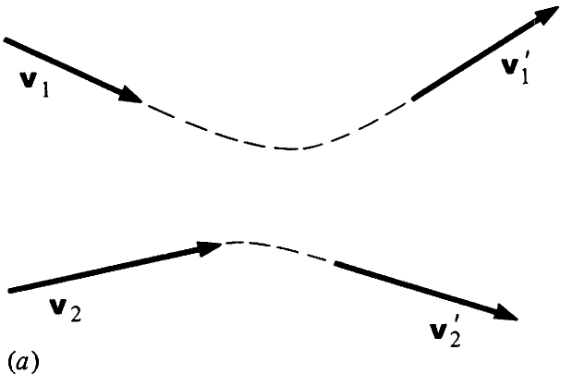
\includegraphics[scale=0.3]{coli1}
  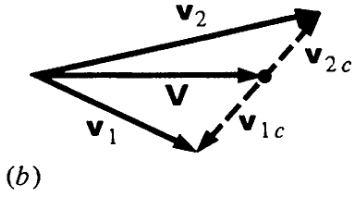
\includegraphics[scale=0.3]{coli2}
  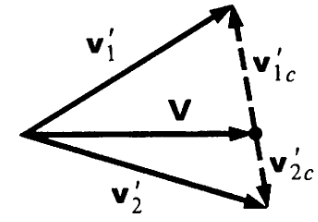
\includegraphics[scale=0.3]{coli3}

\hspace{7cm}{(c)}
  \caption{Colisiones}
  \label{fig:coli}
\end{figure}

La figura~\ref{fig:coli}~(a) muestra las trayectoria y velocidades de
dos partículas en colisión.  
En la figura~\ref{fig:coli}~(b) mostramos las velocidades iniciales en
los sistema $L$ y $C$.
Todos los vectores están sobre el mismo plano.
$\mathbf{v}_{1c}$ y $\mathbf{v}_{2c}$ deben estar espalada con espalda
ya que el moméntum total en el sistema $C$ es cero. 
Después de la colisión, como se muestra en la
figura~\ref{fig:coli}~(c), las velocidades en el sistema $C$ son de
nuevo espalda a espalda. 
La figura también muestra las velocidades
finales en el sistema de laboratorio.
Note que el plano de la figura~\ref{fig:coli}~(c) no es necesariamente
el plano de la figura~\ref{fig:coli}~(a). 
Evidentemente las relaciones geométricas entre las velocidades
iniciales y finales en el sistema $L$ es bastante complicado. 
Afortunadamente, la situación en el sistema $C$ es mucho más simple. 
Las velocidades iniciales y finales en el sistema $C$ determinan un
plano conocido como el plano de dispersión. 
Cada partícula es desviada a través del mismo ángulo de dispersión
$\Theta$ en este plano.

La fuerza de interacción debe ser conocida para poder calcular
$\Theta$, o al contrario, midiendo la desviación podemos aprender
sobre la fuerza de interacción. Sin, embargo evitaremos estas
consideraciones y asumiremos que la interacción ha causado alguna
desviación en el sistema $C$.


Si además la colisión es elástica y denotando con primas las
velocidades después de la colisión tenemos
\begin{align}
\label{eq:cecm}
  \tfrac{1}{2}m_1 v_{1c}^2+  \tfrac{1}{2}m_2 v_{2c}^2
= \tfrac{1}{2}m_1 {v_{1c}'}^2+ \tfrac{1}{2}m_2 {v_{2c}'}^2\,.
\end{align}
Ya que el moméntum inicial y final es cero, y escogiendo
convenientemente el eje $x$ de los sistemas $C$ y $C$, de manera que
coincida con los vectores moméntum, tenemos
\begin{align}
  m_1 v_{1c}+m_2 v_{2c}=&0 \nonumber\\
  m_2 v_{1c}'+m_2 v_{2c}'=&0\,
\end{align}
y
\begin{align}
\label{eq:ccp}
  v_{2c}=&-\frac{m_1}{m_2}v_{1c}\nonumber\\
  v_{2c}'=&-\frac{m_1}{m_2}v_{1c}'\,.
\end{align}
Reemplazando en ec.~(\ref{eq:cecm})
\begin{align}
  m_1 v_{1c}^2+  \frac{m_1^2}{m_2} v_{1c}^2
=& m_1 {v_{1c}'}^2+ \frac{m_1^2}{m_2} {v_{1c}'}^2 \nonumber\\
 \left(m_1+\frac{m_1^2}{m_2}  \right) v_{1c}^2
=&\left(m_1+\frac{m_1^2}{m_2}  \right) {v_{1c}'}^2 \nonumber\\
v_{1c}^2=&{v_{1c}'}^2\,,
\end{align}
de modo que
\begin{align*}
  v_{1c}=&v_{1c}'\,.
\end{align*}
Sustituyendo en la ec.~(\ref{eq:ccp}), obtenemos que
\begin{align*}
  v_{2c}=&v_{2c}'\,.
\end{align*}
En resumen, el problema general de lo colisión de dos cuerpos, visto
desde el sistema del centro de masa, implica que
\begin{align}
  v_{1c}=&v_{1c}'\nonumber\\
  v_{2c}=&v_{2c}'\,.
\end{align}
En una colisión elástica, la rapidez de cada partícula en el sistema
de centro de masa es la misma antes y después de la colisión. Así, los
vectores de velocidad simplemente rotan en el ángulo de dispersión,
como se muestra en la figura~\ref{fig:particolgen}
\begin{figure}
  \centering
  \includegraphics[scale=0.6]{particolgen}
  \caption{Colisión general de dos cuerpos}
  \label{fig:particolgen}
\end{figure}
\begin{inprogress}


\subsection{Ángulo de dispersión}
\end{inprogress}





\section{Problemas resueltos}
\begin{enumerate}
\item Un auto \textbf{A} cuya rapidez es $v_1$ choca con un auto \textbf{B}, cuya rapidez es $v_2$, tal como se muestra en la figura. La masa del auto \textbf{A} es $m$ y la masa del auto \textbf{B} es $6/5$ $m$. Se sabe que los automóviles se aproximaban con cantidads de movimiento de igual magnitud y direcciones opuestas, y que la colisión es elástica, es decir, que la energía cinética del sistema se conserva en la colisión.

  \begin{minipage}{0.4\linewidth}
    \includegraphics[scale=0.7]{colision1}    
  \end{minipage}  \begin{minipage}{0.6\linewidth}
    \begin{enumerate}
    \item Determine  $v_2$ en términos de $v_1$.% y  v'2 en términos de  v'1 .
      \label{item:p1a}
    \item Encuentre la magnitud de las velocidades $v'_1$ y $v'_2$ de cada auto después de la colisión.
      \label{item:p1b}
    \item Calcule las cantidades del literal anterior para  $v_1=10$ m/s. 
      \label{item:p1c}
    \end{enumerate}
  \end{minipage}
\begin{itemize}
\item[\textbf{Solución:}]
  \begin{itemize}
  \item[\ref{item:p1a}]: De la conservación del moméntum, sobe la línea de colisión
    \begin{align*}
      \mathbf{p}_1+\mathbf{p}_2=&0\nonumber\\
      m v_1-\tfrac{6}{5}m v_2=&0\nonumber\\
      v_2=\tfrac{5}{6}v_1
    \end{align*}
  \item[~\ref{item:p1b}]
    El momentúm después de la colisión es cero y por consiguiente
\begin{align*}
  v_2'=\tfrac{5}{6}v_1'\,,
\end{align*}
De la conservación de energía cinética
\begin{align*}
  \tfrac{1}{2}m v_1^2+\tfrac{1}{2}(\tfrac{6}{5}m)  v_2^2=&
  \tfrac{1}{2}m {v_1'}^2+\tfrac{1}{2}(\tfrac{6}{5}m)  {v_2'}^2\nonumber\\
  v_1^2+(\tfrac{5}{6})  v_1^2=&
  {v_1'}^2+(\tfrac{5}{6}) {v_1'}^2\nonumber\\
  \frac{11}{6}{v_1^2}'=&\frac{11}{6}v_1^2\nonumber\\
  {v_1^2}'=&v_1^2\,,
\end{align*}
y entonces
\begin{align*}
 v_2'=\tfrac{5}{6}v_1\,.
\end{align*}

  \end{itemize}

\end{itemize}


\item 

\item (Tomado de \cite{gabriel}) Un bloque de masa $m$ se suelta desde el punto $A$ y este se desliza sobre el cuadrante circular $AB$ de radio $R$, llegando a $B$ con velocidad $v_1$ de acuerdo a la figura. En $B$ choca elásticamente con el bloque de masa $2m$ que se encuentra inicialmente en reposo. Luego del choque, la masa $2m$ se mueve sobre la superficie horizontal lisa hasta chocar y comprimir un resorte de constante elástica $k$. El cuadrante circular AB es rugoso. Calcular

  \begin{minipage}{0.5\linewidth}
    \includegraphics[scale=0.5]{planosuple}
  \end{minipage}
  \begin{minipage}{0.5\linewidth}
    \begin{enumerate}
    \item El trabajo realizado por la fuerza de fricción en el tramo $AB$.
      \label{item:p2a}
    \item La velocidad de cada bloque después del choque.
      \label{item:p2b}
    \item La compresión del resorte.
      \label{item:p2c}
    \item Calcule las cantidades de los literales anteriores para $m=2\ $Kg, $RO=0.5\ $m, $v_1=2.1\ $m/s, $k=1000\ $N/m
    \end{enumerate}
  \end{minipage}

%sln pag 130
  \begin{itemize}
  \item[\textbf{Solución}]
  \item[\ref{item:p2a}]
    \begin{align*}
      W_{ba}=&E_b-E_a\nonumber\\
      =&\tfrac{1}{2}m v_1^2-mgR\,,
    \end{align*}
  \item[\ref{item:p2b}] 
    \begin{align}
      \label{eq:pp2b}
      m v_1=&m v_1'+2m v_2'\\
      \label{eq:pp2bb}
      \tfrac{1}{2}m v_1^2=&\tfrac{1}{2}m {v_1'}^2+\tfrac{1}{2}(2m){v_2'}^2\,.
    \end{align}
    de \eqref{eq:pp2b}
    \begin{align*}
      v_1'=v_1-2v_2'\,,
    \end{align*}
    y en \eqref{eq:pp2bb}
    \begin{align*}
      2{v_2'}^2=&v_1^2-{v_1'}^2\nonumber\\
      =&v_1^2-(v_1^2-4 v_1 v_2'+4{v_2'}^2)\nonumber\\
      =&4v_2'(v_1-v_2')\,.
    \end{align*}
    Simplificando
    \begin{align*}
      v_2'=2v_1-2v_2'\,,
    \end{align*}
    y
    \begin{align*}
      v_2'=\tfrac{2}{3}v_1\,,
    \end{align*}
    además
    \begin{align*}
      v_1'=&v_1-2v_2'\nonumber\\
      =&v_1-\tfrac{4}{3}v_1\nonumber\\
      =&-\tfrac{1}{3}v_1\nonumber\\
    \end{align*}
  \item[\ref{item:p2c}]
    \begin{align*}
      \tfrac{1}{2}(2m){v_2'}^2=&\tfrac{1}{2}kx^2\nonumber\\
       m{v_2'}^2=&\tfrac{1}{2}kx^2\nonumber\\
       mv_2'=&\tfrac{1}{2}\sqrt{k}x\nonumber\\
    \end{align*}
    \begin{align*}
      x=&{v_2'}\sqrt{\frac{2m}{k}}\nonumber\\
      =&\frac{2v_1}{3}\sqrt{\frac{2m}{k}}\,.
    \end{align*}
  \end{itemize}


\item Un anillo resbala a lo largo de un arco metalico ABC muy pulido
  que es arco de una circunferencia de radio
  $R=\SI{1.2}{\meter}$. 
  Sobre el anillo actúa una fuerza $\mathbf{F}$ de magnitud
  $\SI{150}{\newton}$ y dirección constante formando un ángulo de
  $\alpha=\pi/6$ con la horizontal.

  \begin{minipage}{0.5\linewidth}
   \includegraphics[scale=0.5]{anillos}
  \end{minipage}
  \begin{minipage}{0.5\linewidth}
    Calcular el trabajo efectuado por la fuerza $\mathbf{F}$ sobre el anillo al moverse desde $A$ a $B$ y de $B$ a $C$
  \end{minipage}
  \begin{itemize}
  \item[\textbf{Solución}]
    En la figura se muestra el anillo en una posición general, de la figure tenemos que en el sistema de coordenadas $\hat{\mathbf{r}}$-$\hat{\boldsymbol{\theta}}$:
    \begin{align*}
      \mathbf{F}=F_r \hat{\mathbf{r}}+F_\theta\hat{\boldsymbol{\theta}}\,,
    \end{align*}
    donde
    \begin{align*}
      F_\theta=&F\cos(\pi/2-\theta+\alpha)\nonumber\\
      =&F\sin(\alpha-\theta)\,. %comprobar
    \end{align*}

    Además del próximo capítulo:
    \begin{align*}
      \frac{d\mathbf{r}}{dt}=\frac{dr}{dt} \hat{\mathbf{r}}+ r\frac{d\theta}{dt}\hat{\boldsymbol{\theta}}\,,
    \end{align*}
    de modo que
    \begin{align*}
      d\mathbf{r}=dr \hat{\mathbf{r}}+ r \, d\theta\hat{\boldsymbol{\theta}}\,.
    \end{align*}
    Por la simetría del problema el trabajo para ir de $A$ a $C$ es el doble de ir de $A$ a $B$, además, como el movimiento sólo de da a lo largo de dirección tangencail al arco, entonces sólo la componente tangencial de la fuerza realiza trabajo. Con todas estas consideraciones tenemos:
    \begin{align*}
      W_{AC}=2W_{AB}=&\int_A^B \mathbf{F}\cdot d\mathbf{r}\nonumber\\
      =&2\int_A^B (F_r\hat{\mathbf{r}}+F_\theta\hat{\boldsymbol{\theta}})\cdot (dr \hat{\mathbf{r}}+ r \, d\theta\hat{\boldsymbol{\theta}})\nonumber\\
      =&2\int_A^B (F_\theta r \, d\theta)\hat{\boldsymbol{\theta}}\cdot\hat{\boldsymbol{\theta}}\nonumber\\
      =&2\int_{0}^{\pi/2}F_\theta r \, d\theta\nonumber\\
      =&2Fr\int_{0}^{\pi/2}\sin(\alpha-\theta) \, d\theta\nonumber\\
      =&2Fr\cos(\alpha-\theta)|_0^{\pi/2}\nonumber\\
      =&2Fr[\sin(\alpha-\pi/2)-\sin(\pi/6)]\nonumber\\
      =&\SI{131.77}{\joule}\,.
    \end{align*}

   
  \end{itemize}



\item ...
  \begin{minipage}{0.5\linewidth}
    ...
  \end{minipage}
  \begin{minipage}{0.5\linewidth}
    ...
  \end{minipage}
  \begin{itemize}
  \item[\textbf{Solución}]
  \item[iref]
  \end{itemize}
\end{enumerate}

%%% Local Variables: 
%%% mode: latex
%%% TeX-master: "mecanica"
%%% End: 


\chapter{Movimiento circular}
\label{chap:cin1}



% \subsection{Caida libre}
% La observaci\'on experimental, como por ejemplo la caida de una pluma y un bal\'\i n en un tubo de vacio, han establecido que todos los objetos cerca a la tierra se aceleran al la misma tasa constante cuando otros efectos externos est\'an excluidos.


% En un sistema de coordenadas donde la direcci\'on de movimiento es perpendicular a la superficie de la tierra, podemos definir un \emph{vector unitario}, es decir, un vector de magnitud 1 y direcci\'on positiva como $\hat{\mathbf{j}}$, tal que
% \begin{align}
%   |\hat{\mathbf{j}}| = 1,
% \end{align}
% donde los simbolos $|\ |$ representan la magnitud del vector. Entonces el vector de aceleraci\'on gravitacional se puese escribir como
% \begin{align}
%   \mathbf{a}=-g \hat{\mathbf{j}}\,.
% \end{align}

% Los vectores se denotan con letra negrilla o con una flecha arriba $\vec a$. Usaremos la primera opci\'on en este texto. La magnitud del vector de aceleraci\'on gravitacional es entonces:
% \begin{align}
%   |\mathbf{a}|=g=9.8\ \frac{\text{m}}{\text{s}}
% \end{align}

% La soluci\'on a la ecuaci\'on de movimiento
% \begin{align}
%   \frac{d^2y(t)}{dt^2}=-g\,,
% \end{align}

% % ver notas Kowalaski 3-11


\section{Movimiento Circular Uniforme}

Considere el movimiento descrito por la siguiente ecuaci\'on
\begin{align}
  \label{eq:mua}
  \mathbf{r}(t)=r\left(\hat{\mathbf{i}}\cos(\omega t)+\hat{\mathbf{j}}\sin(\omega t)\right),
\end{align}
con $r=\text{constante}$ y $\omega=\text{constante}$, representado en la figura~\ref{fig:mua1}.

La velocidad es
\begin{align}
  \mathbf{v}=&%detalles\\
  r\omega\left(-\hat{\mathbf{i}}\sin(\omega t)+\hat{\mathbf{j}}\cos(\omega t)\right),
\end{align}
representado en la figura~\ref{fig:mua2}. Note que $\mathbf{r}\cdot\mathbf{v}=0$, de modo que los vectores son perpendiculares.

La aceleraci\'on es
\begin{align}
  \mathbf{a}=&%detalles\\
  -r\omega^2\left(\hat{\mathbf{i}}\cos(\omega t)+\hat{\mathbf{j}}\sin(\omega t)\right),
\end{align}
representado en la figura~\ref{fig:mua3}. Note que $\mathbf{a}\cdot\mathbf{v}=0$, de modo que los vectores son perpendiculares. Adem\'as
$\mathbf{r}\cdot\mathbf{a}=-1$, de modo que los vectores son antiparalelos.


\begin{frame}[fragile,allowframebreaks]
  \begin{figure}
    \centering
    \includegraphics[scale=0.65]{mua1}    
    \caption{Posici\'on}
    \label{fig:mua1}
  \end{figure}

\end{frame}
\begin{frame}[fragile,allowframebreaks]
  \begin{figure}
    \centering
    \includegraphics[scale=0.65]{mua2}    
    \caption{Velocidad: tangente a la curva}
    \label{fig:mua2}
  \end{figure}
\end{frame}

\begin{frame}[fragile,allowframebreaks]
  \begin{figure}
    \centering
    \includegraphics[scale=0.65]{mua3}
    \caption{Aceleraci\'on: centr\'\i peta}
    \label{fig:mua3}
  \end{figure}


\end{frame}

\subsection{Movimiento generalizado en coordenadas polares}
La ecuaci\'on para el vector de posici\'on puede escribirse en general como
\begin{align}
\label{eq:rpol}
  \mathbf{r}(t)=r(t)\left(\hat{\mathbf{i}}\cos[\theta(t)]+\hat{\mathbf{j}}\sin[\theta(t)]\right)\,.
\end{align}
Para algunos problemas es conveniente reescribir \'esta ecauaci\'on en coordenadas polares:
\begin{inprogress}
  Faltan detalles
\end{inprogress}
\begin{align}
  \label{eq:polinv}
  \begin{pmatrix}
    \hat{\mathbf{r}}\\
    \hat{\boldsymbol{\theta}}
  \end{pmatrix}=
  \begin{pmatrix}
    \cos\theta&-\sin\theta\\
    \sin\theta&\cos\theta\\
  \end{pmatrix}
  \begin{pmatrix}
    \;\hat{\mathbf{i}}\;\\
    \hat{\mathbf{j}}\\
  \end{pmatrix}.
\end{align}
con inverso
\begin{align}
  \begin{pmatrix}
    \;\hat{\mathbf{i}}\;\\
    \hat{\mathbf{j}}\\
  \end{pmatrix}=
  \begin{pmatrix}
    \cos\theta&-\sin\theta\\
    \sin\theta&\cos\theta\\
  \end{pmatrix}
  \begin{pmatrix}
    \hat{\mathbf{r}}\\
    \hat{\boldsymbol{\theta}}
  \end{pmatrix}.
\end{align}

La velocidad es
\begin{align}
  \label{eq:vpol}
  \mathbf{v}(t)=&%detalles\\
  \dot{r}(t)\hat{\mathbf{r}}(t)+r(t)\dot{\theta}(t)\hat{\boldsymbol{\theta}}(t)\,.
\end{align}
y la aceleraci\'on es
\begin{align}
\label{eq:apol}
  \mathbf{a}(t)=&%detalles\\
[\underbrace{\ddot{r}(t)}_{{\text{Acel. lineal.}}}
-\underbrace{r(t)\dot{\theta}^2(t)}_{{\text{Acel. centr\'\i peta.}}}]\hat{\mathbf{r}}(t)
+[\underbrace{r(t)\ddot{\theta}(t)}_{{\text{Acel. lineal tangencial.}}}
+\underbrace{2\dot{r}(t)\dot{\theta}(t)}_{{\text{Acel. de coriolis.}}}]\hat{\boldsymbol{\theta}}(t).
\end{align}
\begin{itemize}
\item[\textbf{Ejemplo}] \textbf{MCU}:\\
Comparando (\ref{eq:mua}) con (\ref{eq:rpol}), tenemos para el Movimiento Circular Uniforme que
\begin{align}
  \label{eq:muapol}
   \dot{r}=&0&&&&\\
  \theta(t)=&\omega t\,,&\dot{\theta}(t)=&\omega\,,&\ddot{\theta}(t)=&0\,.
\end{align}
De modo que reemplazando las ecuaciones \eqref{eq:muapol} en las ecuaciones \eqref{eq:vpol}, \eqref{eq:apol}, y usando la transformaci\'on inversa \eqref{eq:polinv}, tenemos que
\begin{align}
  \mathbf{r}(t)=&r\hat{\mathbf{r}}(t)\nonumber\\
  =&r\left(\hat{\mathbf{i}}\cos(\omega t)+\hat{\mathbf{j}}\sin(\omega t)\right),
\end{align}
\begin{align}
    \mathbf{v}(t)=&r\omega\hat{\boldsymbol{\theta}}(t)\nonumber\\
    =&r\omega\left(-\hat{\mathbf{i}}\sin(\omega t)+\hat{\mathbf{j}}\cos(\omega t)\right),
\end{align}
\begin{align}
  \mathbf{a}(t)=&-r\omega^2\hat{\mathbf{r}}(t)\nonumber\\
  =&-r\omega^2\left(\hat{\mathbf{i}}\cos(\omega t)+\hat{\mathbf{j}}\sin(\omega t)\right),
\end{align}
de modo que en el MCU la velocidad no tiene componente radial, y s\'olo
contribuye la aceleraci\'on centr\'\i peta, como era de esperarse.
\end{itemize}

Continuara...

%\left(\right)
%ver inkscape vectores primera capa






%%% Local Variables: 
%%% mode: latex
%%% TeX-master: "mecanica"
%%% End: 



\chapter{Movimiento del cuerpo rígido}

\section{Movimiento Circular Uniforme I}


Considere el movimiento de un objeto atado a una cuerda que es forzado a girar en un plano horizontal. Queremos encontrar determinar la tensión de la cuerda en función de la rapidez y el radio de giro. Si la rapidez es constante el movimiento está descrito por la siguiente ecuación
%%Modificar en adelante de acuerdo a este discurso
\begin{align}
  \label{eq:mua}
  \mathbf{r}(t)=r\left[\hat{\mathbf{i}}\cos(\omega t)+\hat{\mathbf{j}}\sin(\omega t)\right],
\end{align}
con $r=\text{constante}$ y $\omega=\text{constante}$, representado en la figura~\ref{fig:mua1}.

La velocidad es
\begin{align}
  \mathbf{v}=&%detalles\\
  r\omega\left[-\hat{\mathbf{i}}\sin(\omega t)+\hat{\mathbf{j}}\cos(\omega t)\right],
\end{align}
representado en la figura~\ref{fig:mua2}. Note que, 
\begin{align*}
\mathbf{r}\cdot\mathbf{v}=r^2\omega 
   \left[-\sin(\omega t)\cos(\omega t)+\sin(\omega t)\cos(\omega t) \right]
  =0\,,
\end{align*}
de modo que los vectores son perpendiculares entre sí.

La aceleración es
\begin{align}
  \mathbf{a}=&%detalles\\
  -r\omega^2\left[\hat{\mathbf{i}}\cos(\omega t)+\hat{\mathbf{j}}\sin(\omega t)\right],
\end{align}
representado en la figura~\ref{fig:mua3}. Note que
\begin{align*}
  \mathbf{a}\cdot\mathbf{v}=r^2\omega^3 
   \left[-\sin(\omega t)\cos(\omega t)+\sin(\omega t)\cos(\omega t) \right]
  =0\,,
\end{align*}
de modo que los vectores son perpendiculares. Además 
$\mathbf{r}\cdot\mathbf{a}=-1$, de modo que los vectores son antiparalelos.


\begin{frame}[fragile,allowframebreaks]
  \begin{figure}
    \centering
    \includegraphics[scale=0.65]{mua1}    
    \caption{Posici\'on}
    \label{fig:mua1}
  \end{figure}

\end{frame}
\begin{frame}[fragile,allowframebreaks]
  \begin{figure}
    \centering
    \includegraphics[scale=0.65]{mua2}    
    \caption{Velocidad: tangente a la curva}
    \label{fig:mua2}
  \end{figure}
\end{frame}

\begin{frame}[fragile,allowframebreaks]
  \begin{figure}
    \centering
    \includegraphics[scale=0.65]{mua3}
    \caption{Aceleraci\'on: centr\'\i peta}
    \label{fig:mua3}
  \end{figure}


\end{frame}

\subsection{Movimiento generalizado en coordenadas polares}

%Hacer una figura con los ejes rotados con hat theta a pi/2+theta 

Para algunos problemas en dos dimensiones, es conveniente reescribir el vector de posición $\mathbf{r}(t)=x(t)\hat{\mathbf{i}}+y(t)\hat{\mathbf{j}}$ en términos de coordenadas polares:

\begin{frame}
\noindent
\begin{minipage}{0.2\textwidth}
\includegraphics[scale=1]{polares}  
\end{minipage}
\begin{minipage}{0.8\textwidth}
  \begin{align}
    \label{eq:polares}
    x(t)=&r(t)\cos \left[ \theta(t) \right]\nonumber\\
    y(t)=&r(t)\sin \left[ \theta(t) \right]
  \end{align}
\end{minipage}
\end{frame}


La ecuaci\'on para el vector de posici\'on puede escribirse en general como
\begin{align}
\label{eq:rpol}
  \mathbf{r}(t)=&r(t)\left\{\hat{\mathbf{i}}\cos[\theta(t)]+\hat{\mathbf{j}}\sin[\theta(t)]\right\}\nonumber\\
=&r(t)\hat{\mathbf{r}}(t)\,,
\end{align}
donde
\begin{align}
\label{eq:runit}
  \hat{\mathbf{r}}(t)=\hat{\mathbf{i}}\cos[\theta(t)]+\hat{\mathbf{j}}\sin[\theta(t)]\,.
\end{align}


El vector perpendicular a $\hat{\mathbf{r}}(t)$ describe la dirección angular. De la figura %ver notas
\begin{align}
\label{eq:thetaunit}
  \hat{\boldsymbol{\theta}}(t)=&\hat{\mathbf{i}}\cos[\theta(t)+\pi/2]+\hat{\mathbf{j}}\sin[\theta(t)+\pi/2]\nonumber\\
=&-\hat{\mathbf{i}}\sin[\theta(t)]+\hat{\mathbf{j}}\cos[\theta(t)]\,.
\end{align}

Las ecuaciones \eqref{eq:runit} y \eqref{eq:thetaunit} pueden escribirse en forma matricial


\begin{align}
  \label{eq:polinv}
  \begin{pmatrix}
    \hat{\mathbf{r}}\\
    \hat{\boldsymbol{\theta}}
  \end{pmatrix}=
  \begin{pmatrix}
    \cos\theta&\sin\theta\\
    -\sin\theta&\cos\theta\\
  \end{pmatrix}
  \begin{pmatrix}
    \;\hat{\mathbf{i}}\;\\
    \hat{\mathbf{j}}\\
  \end{pmatrix}.
\end{align}
con inverso
\begin{align}
  \begin{pmatrix}
    \;\hat{\mathbf{i}}\;\\
    \hat{\mathbf{j}}\\
  \end{pmatrix}=
  \begin{pmatrix}
    \cos\theta&-\sin\theta\\
    \sin\theta&\cos\theta\\
  \end{pmatrix}
  \begin{pmatrix}
    \hat{\mathbf{r}}\\
    \hat{\boldsymbol{\theta}}
  \end{pmatrix}.
\end{align}

De la ec.~\eqref{eq:rpol}, la velocidad es
\begin{align}
  \label{eq:vcurvprev}
  \mathbf{v}(t)=\dot{\mathbf{r}}(t)=\dot{r}(t)\hat{\mathbf{r}}(t)+
r(t)\dot{\hat{\mathbf{r}}}(t)\,.
\end{align}
Ahora, de la ec.~\eqref{eq:runit}
\begin{align}
  \dot{\hat{\mathbf{r}}}(t)=&\frac{d}{dt}\left(\hat{\mathbf{i}}\cos[\theta(t)]+\hat{\mathbf{j}}\sin[\theta(t)]\right)\nonumber\\
  =&\dot{\theta}
  \left(
    -\hat{\mathbf{i}}\sin[\theta(t)]+\hat{\mathbf{j}}\cos[\theta(t)]
  \right)
\end{align}
y usando la ec.~\eqref{eq:thetaunit}
\begin{align}
\label{eq:dhr}
\dot{\hat{\mathbf{r}}}(t)=\dot{\theta}\hat{\boldsymbol{\theta}}\,.
\end{align}
Sustituyendo en la ec.~\eqref{eq:vcurvprev}:
\begin{align}
  \label{eq:vpol}
  \mathbf{v}(t)=&\dot{r}(t)\hat{\mathbf{r}}(t)+r(t)\dot{\theta}(t)\hat{\boldsymbol{\theta}}(t)\nonumber\\
  =&\dot{r}(t)\hat{\mathbf{r}}(t)+r(t)\omega(t)\hat{\boldsymbol{\theta}}(t)\,.
\end{align}
donde hemos definido la velocidad angular instantánea como
\begin{align}
  \omega(t)=\dot\theta(t)\,.
\end{align}
Además
\begin{align}
\label{eq:dht}
  \dot{\hat{\boldsymbol{\theta}}}(t)=&
  -\hat{\mathbf{i}}\dot{\theta}(t)\cos[\theta(t)]-\hat{\mathbf{j}}\dot{\theta}(t)\sin[\theta(t)]\nonumber\\
  =&-\hat{\mathbf{r}}(t)\,.
\end{align}

Usando (\ref{eq:vpol}) con (\ref{eq:dhr})  y (\ref{eq:dht}), la aceleraci\'on es %ver notas
\begin{align}
\label{eq:apol}
  \mathbf{a}(t)=&\frac{d\mathbf{v}(t)}{dt}\nonumber\\
=& \ddot{r}(t)\hat{\mathbf{r}}(t)+\dot{r}(t)\dot{\hat{\mathbf{r}}}(t)+\dot{r}(t)\dot{\theta}(t)\hat{\boldsymbol{\theta}}(t)
+r(t)\ddot{\theta}(t)\hat{\boldsymbol{\theta}}(t)
+r(t)\dot{\theta}(t)\dot{\hat{\boldsymbol{\theta}}}(t) \nonumber\\
=&
 \ddot{r}(t)\hat{\mathbf{r}}(t)+\dot{r}(t)\dot{\theta}(t)\hat{\boldsymbol{\theta}}(t)+\dot{r}(t)\dot{\theta}(t)\hat{\boldsymbol{\theta}}(t)
+r(t)\ddot{\theta}(t)\hat{\boldsymbol{\theta}}(t)
-r(t)\dot{\theta}(t)\dot{\theta}(t)\hat{\mathbf{r}} \nonumber\\
=&[\underbrace{\ddot{r}(t)}_{{\text{Acel. lineal.}}}
-\underbrace{r(t)\dot{\theta}^2(t)}_{{\text{Acel. centr\'\i peta.}}}]\hat{\mathbf{r}}(t)
+[\underbrace{r(t)\ddot{\theta}(t)}_{{\text{Acel. lineal tangencial.}}}
+\underbrace{2\dot{r}(t)\dot{\theta}(t)}_{{\text{Acel. de coriolis.}}}]\hat{\boldsymbol{\theta}}(t).
\end{align}

\begin{frame}
  En resumen, en coordenadas polares $\hat{\mathbf{r}}$, $\hat{\boldsymbol{\theta}}$ la velocidad y la aceleración están dadas por
\begin{align*}
   \mathbf{v}(t)=&\dot{\mathbf{r}}(t)=\dot{r}(t)\hat{\mathbf{r}}(t)+
r(t)\dot{\hat{\mathbf{r}}}(t)\nonumber\\
 \mathbf{a}(t)=&
\left[\ddot{r}(t)-r(t)\dot{\theta}^2(t)\dot{\theta}(t)\right]\hat{\mathbf{r}} 
+\left[r(t)\ddot{\theta}(t)+2\dot{r}(t)\dot{\theta}(t)  \right]\hat{\boldsymbol{\theta}}(t)
\end{align*}
\end{frame}

\subsection{Vector de velocidad angular}

Es conveniente definir un espacio tridimensional asignando un vector unitario,
$\hat{\boldsymbol{\omega}}$, perpendicular al plano en coordenadas polares
$\hat{\mathbf{r}}$, $\hat{\boldsymbol{\theta}}$, tal que
\begin{align*}
  \hat{\boldsymbol{\omega}}=\hat{\mathbf{r}}\times \hat{\boldsymbol{\theta}}\,.
\end{align*}
Entonces
\begin{align*}
 \hat{\boldsymbol{\theta}}=&\hat{\boldsymbol{\omega}}\times\hat{\mathbf{r}}& \hat{\mathbf{r}}=&\hat{\boldsymbol{\theta}}\times\hat{\boldsymbol{\omega}}\,.
\end{align*}
De esta formula, la ecuación para la velocidad en coordenadas polares \eqref{eq:vpol}, puede escribirse como
\begin{align}
    \mathbf{v}(t)
  =&\dot{r}(t)\hat{\mathbf{r}}(t)+r(t)\omega(t)\hat{\boldsymbol{\theta}}(t)\nonumber\\
  =&\frac{\dot{r}(t)}{r(t)}r(t)\hat{\mathbf{r}}(t)+r(t)\omega(t)\hat{\boldsymbol{\omega}}\times\hat{\mathbf{r}}\nonumber\\
  =&\frac{\dot{r}(t)}{r(t)}\mathbf{r}(t)+\boldsymbol{\omega}(t)\times\mathbf{r}(t)\,,
\end{align}
donde hemos identificado la dirección perpendicular al plano $\hat{\mathbf{r}}$-$\hat{\boldsymbol{\theta}}$, con la dirección de la velocidad angular
\begin{align}
  \boldsymbol{\omega}(t)=\omega(t)\hat{\boldsymbol{\omega}}(t)\,.
\end{align}




Las componentes angulares como tal:
\begin{align*}
  \theta_x\hat{\mathbf{i}}+\theta_y\hat{\mathbf{j}}+\theta_k\hat{\mathbf{k}}\,,
\end{align*}
no pueden formar un vector, pues no resultaria ser conmutativo, como
puede mostrarse facilmente haciendo rotaciones sobre los tres ejes de
un libro en el espacio. La diferencia entre las diferentes
posibilidades de rotaciones son del orden de $\Delta
\theta_{x,y,x}^2$, de modo que las componentes diferenciales si forman
un vector. 

Definimos entonces la velocidad angular en tres dimensiones como:
\begin{align}
  \boldsymbol{\omega}=&\frac{d\theta_x}{dt}\hat{\mathbf{i}}+\frac{d\theta_y}{dt}\hat{\mathbf{j}}
+\frac{d\theta_z}{dt}\hat{\mathbf{k}}\nonumber\\
=&\omega_x\hat{\mathbf{i}}+\omega_y\hat{\mathbf{j}}+\omega_z\hat{\mathbf{k}}\,,
\end{align}
la cual si constituye un vector.

\subsection{Movimiento circular uniforme II}


Una partícula en movimiento circular uniforme (MCU), dado por la ec.~\eqref{eq:muapol}, mantiene el radio del movimiento constante con respecto a un sistema de referencia en el centro de giro. Por lo tanto, en coordenadas polares dicho movimiento satisface que
\begin{align}
  \label{eq:muapol}
   \dot{r}=&0&&&&\\
  \theta(t)=&\omega t\,,&\dot{\theta}(t)=&\omega\,,&\ddot{\theta}(t)=&0\,.
\end{align}
De modo que reemplazando las ecuaciones  en las ecuaciones \eqref{eq:vpol}, \eqref{eq:apol}, y usando la transformaci\'on inversa \eqref{eq:polinv}, tenemos que
\begin{align}
  \mathbf{r}(t)=&r\hat{\mathbf{r}}(t)\nonumber\\
  =&r\left(\hat{\mathbf{i}}\cos(\omega t)+\hat{\mathbf{j}}\sin(\omega t)\right),
\end{align}
\begin{align}
    \mathbf{v}(t)=&r\omega\hat{\boldsymbol{\theta}}(t)\nonumber\\
    =&r\omega\left(-\hat{\mathbf{i}}\sin(\omega t)+\hat{\mathbf{j}}\cos(\omega t)\right),
\end{align}
en magnitud:
\begin{align}
  \label{eq:vome}
  v=r\omega\,.
\end{align}

La siguiente derivada da lugar a 
\begin{align*}
  \mathbf{a}(t)=\dot{\mathbf{v}}(t)=&-r(t)\omega^2(t)\hat{\mathbf{r}}(t)\nonumber\\
  =&-\frac{(r\omega)^2}{r}\hat{\mathbf{r}}\,,
\end{align*}
y usando la ec.\eqref{eq:vome}
\begin{align}
\label{eq:muaa}
  \mathbf{a}(t)=-\frac{v^2}{r}\hat{\mathbf{r}}
\end{align}

de modo que en el MCU la velocidad no tiene componente radial, y s\'olo
contribuye la aceleraci\'on centr\'\i peta, como era de esperarse.
\ejemplo{\textbf{MCU}:}
Calcule la fuerza para mantener un cuerpo de masa $m$ en un movimiento circular uniforme


Tenemos que la ec.~\eqref{eq:muaa} da lugar a
\begin{align}
  \mathbf{F}=m\mathbf{a}=-\frac{m v^2}{r}\hat{\mathbf{r}}\,.
\end{align}


\qed

%theta es theta_z y la direccion de omega_z es a lo largo del eje z


\ejemplo{} 
\label{eje:movim-gener-en}
Calcular la velocidad de rotación de una partícula 
girando en movimiento circular en una plano paralelo al plano $x$-$y$
y con el eje $z$ pasando por el centro de la orbita circular.

%hacer dibujo obtener la formula para la velocidad en términos de la
%velocidad angular.  ver notas en estrellitas
\qed


\section{Momento angular y torque para una partícula}
Como último caso de aplicación del teorema de Noether, debemos
preguntarnos cual es la cantidad conservada asociada a la isotropía
del espacio, es decir con la invarianza de la leyes de la naturaleza
con respecto a rotaciones en el espacio: si realizamos un experimento
sobre una mesa, y luego lo repetimos con la mesa rotada en algún
ángulo sobre un eje perpendicular a la superficie, entonces el resultado
del experimento debe ser el mismo.

La cantidad conservada es más fácil de visualizar en el caso de la
rotación de un cuerpo rígido, es decir, un cuerpo dentro del cual
todas la partículas que lo componen mantienen su posición de manera
que el cuerpo siempre esta cohesionado. 
De este modo, dentro un cuerpo rígido en rotación con respecto a algún
eje todas la partículas se mueven con la misma velocidad angular
$\boldsymbol{\omega}$.
Cuando observamos un cuerpo rígido girando con respecto a un
\emph{sólo} eje de giro como la rueda de una bicicleta, un yoyó, un
trompo, etc; podemos ver que la dirección del eje de giro se opone al
cambio de dirección. 
En particular la conservación del eje de giro de las ruedas es lo que
garantiza el equilibrio de una bicicleta en movimiento.


La cantidad conservada entonces debe ser una cantidad proporcional al
vector $\boldsymbol{\omega}$ asociada con el giro de una de la
partículas que compone el cuerpo rígido. 
Como por definición el radio de giro de tal partícula es constante,
entonces la combinación de cantidades vectoriales relevante debe ser
alguna de las combinaciones entre $\mathbf{r}$, $\mathbf{v}$ y
$\boldsymbol{\mathbf{\omega}}$ (tal que usando la regla de la mano
derecha, la mano se debe enrollar de $\mathbf{r}$ a $\mathbf{v}$ para
definir $\boldsymbol{\Omega}$)
\begin{align*}
  \mathbf{v}=\boldsymbol{\omega}\times\mathbf{r}\,,\qquad
  \mathbf{r}=\mathbf{v}\times\boldsymbol{\omega}\,,\qquad
  \boldsymbol{\omega}=\mathbf{r}\times\mathbf{v}\,.
\end{align*}
Asumimos entonces que la cantidad conserva es proporcional al vector
de velocidad angular, y la definimos de manera que el factor de
proporcionalidad sea la masa de la partícula:
$m(\mathbf{r}\times\mathbf{v})=\mathbf{r}\times\mathbf{p}$. 

Comencemos entonces definiendo el momento angular para una partícula de moméntum $\mathbf{p}$ como
\begin{align}
  \label{eq:L}
  \mathbf{L}=&\mathbf{r}\times\mathbf{p}\,.
\end{align}
y el correspondiente vector de torque como el causante de los cambios
en el momento angular cuando es aplicado durante algún intervalo
$\Delta t$ sobre la partícula. 

Podemos establecer entonces el \emph{principio de momento angular}
para una partícula como
\begin{align}
  \Delta \mathbf{L}\approx \boldsymbol{\tau}\Delta t\,.
\end{align}
donde $\boldsymbol{\tau}$ es el torque aplicado sobre la partícula. 

En forma diferencial el principio de momento angular puede escribirse como
\begin{align}
\label{eq:tautor}
  \boldsymbol{\tau}=\frac{d\,\mathbf{L}}{dt}\,.
\end{align}
Desarrollando esta expresión, tenemos que
\begin{align}
  \boldsymbol{\tau}=&\frac{d}{dt}\left(\mathbf{r}\times\mathbf{p}\right)\nonumber\\
=&\left(\frac{d\mathbf{r}}{dt}\right)\times\mathbf{p}+
\mathbf{r}\times\frac{d\mathbf{p}}{dt}\nonumber\\
=&\mathbf{v}\times\mathbf{p}+
\mathbf{r}\times\frac{d\mathbf{p}}{dt}\nonumber\\
\end{align}
como $\mathbf{v}$ es paralelo a $\mathbf{p}$,
$\mathbf{v}\times\mathbf{p}=0$, y teniendo en cuenta que la variación
del momentum es la fuerza aplicada, $\mathbf{F}$, entonces
\begin{align}
  \label{eq:torqueini}
  \boldsymbol{\tau}=\mathbf{r}\times\mathbf{F}\,.
\end{align}

Para entender las definiciones de momento angular y torque es mejor
ir hacia atrás del resultado en \eqref{eq:torqueini} al resultado en
\eqref{eq:L}: La capacidad de una fuerza para ejercer un giro sobre
una partícula depende de la distancia a la que es aplicada la fuerza.
%\left(\right)

\section{momento angular para un cuerpo rígido}


El momento angular para un cuerpo rígido es la suma del momentum
angular para cada partícula dentro del cuerpo rígido como se ilustra
en la fig.~\ref{fig:centrodemasarigido}

\begin{frame}
\begin{figure}
  \centering
  \includegraphics{centrodemasarigido}
  \caption{Cuerpo rígido}
  \label{fig:centrodemasarigido}
\end{figure}
\end{frame}
\begin{align}
  \mathbf{L}_{\text{total}}=\sum_{i=1}^N\mathbf{L}_i=\sum_{i=1}^N \mathbf{r}_i\times m_i\dot{\mathbf{r}}_i
\end{align}
Usando la relación entre las coordenas con respecto a una sistema
externo y las coordenadas del centro de masa
\begin{align}
  \mathbf{r}_i=\mathbf{R}+\mathbf{r}_i'\,,
\end{align}

\begin{align}
   \mathbf{L}_{\text{total}}=&\sum_{i=1}^N
   \left(\mathbf{R}+\mathbf{r}_i'\right)\times m_i
   \left(\dot{\mathbf{R}}+\dot{\mathbf{r}}_i'\right)
\end{align}
Analicemos término a término
\begin{enumerate}
\item 
\begin{align*}
  \sum_{i=1}^N\mathbf{R}\times m_i\dot{\mathbf{R}}=&\mathbf{R}\times
  \left(\sum_{i=1}^N m_i\right)\dot{\mathbf{R}}\nonumber\\
  =&\mathbf{R}\times M\mathbf{V}\nonumber\\
  =&\mathbf{R}\times \mathbf{P}\nonumber\\
  =&\mathbf{L}_{\text{orb}}\,,
\end{align*}
donde $\mathbf{P}$ es el moméntum lineal total del cuerpo rígido con
respecto al centro de masa y el momento angular orbital,
$\mathbf{L}_{\text{orb}}$, es momento angular ocasionado por las
fuerzas externas al cuerpo rígido
\item
  \begin{align}
    \label{eq:rmr}
    \sum_{i=1}^N\mathbf{r}_i'\times m_i \dot{\mathbf{R}}
    =&\sum_{i=1}^N m_i\left(\mathbf{r}_i-\mathbf{R}\right)\times  \dot{\mathbf{R}}\nonumber\\
    =&\left(M\frac{\sum_{i=1}^N m_i\mathbf{r}_i}{M}- M \mathbf{R}\right)\times  \dot{\mathbf{R}}\nonumber\\
    =&\left(M\mathbf{R}- M \mathbf{R}\right)\times  \dot{\mathbf{R}}\nonumber\\
    =&\mathbf{0}\,.
  \end{align}
  %
\item
  \begin{align*}
    \sum_{i=1}^N \mathbf{R}\times m_i \dot{\mathbf{r}}_i'=0\,.
  \end{align*}
\item
  \begin{align*}
    \sum_{i=1}^N \mathbf{r}_i'\times m_i \dot{\mathbf{r}}_i'=&
    \sum_{i=1}^N \mathbf{r}_i'\times m_i \mathbf{v}_i'\nonumber\\
    =&\mathbf{L}_0\,,
  \end{align*}
donde hemos definido el momento angular intrínseco del cuerpo rígido $\mathbf{L}_0$


\end{enumerate}

Entonces el momento angular total puede  escribirse en el sistema de centro de masa, $\mathbf{r}_i'$, como 
\begin{align}
  \label{eq:lcm}
   \mathbf{L}_{\text{total}}=&\mathbf{L}_{\text{orb}}+\mathbf{L}_0\nonumber\\
   =&\mathbf{R}\times M\mathbf{V}+\sum_{i=1}^N \mathbf{r}_i'\times m_i\dot{\mathbf{r}}_i'\,,
\end{align}
\noindent
\textbf{Teorema}: Desarrollando está expresión se puede obtener
\begin{align}
  \label{eq:tensorI}
  \mathbf{L}_{\text{total}}=\mathbf{R}\times M\mathbf{V}+\mathbb{I}\boldsymbol{\omega}\,,
\end{align}
donde $\mathbb{I}$ es el tensor de inercia. 
\medskip

\noindent
\textbf{Demostración}
\begin{align*}
\mathbf{L}_0 =& \sum_{i=1}^N \mathbf{r}_i'\times
m_i\dot{\mathbf{r}}_i' \nonumber\\
=&  \sum_{i=1}^N \mathbf{r}_i'\times m_i\dot{\mathbf{v}}_i' \nonumber\\
=&  \sum_{i=1}^N \mathbf{r}_i'\times m_i (\boldsymbol{\omega}\times \mathbf{r}'_i)
\end{align*}
Usando la identidad
\begin{align*}
  \mathbf{A}\times\left(\mathbf{B}\times\mathbf{C}\right)=\left(\mathbf{A}\cdot\mathbf{C}\right)\mathbf{B}-\left(\mathbf{A}\cdot\mathbf{B}\right)\mathbf{C}
\end{align*}
tenemos para $\mathbf{A}=\mathbf{C}=\mathbf{r}_i$ y
$\mathbf{B}=\boldsymbol{\omega}$, que
\begin{align*}
  \mathbf{L}_0=&\sum_{i=1}^N m_i \left[ \left(\mathbf{r}_i'\cdot\mathbf{r}_i'
  \right)\boldsymbol{\omega}
  -\left( \mathbf{r}_i'\cdot\boldsymbol{\omega}\right)\mathbf{r}_i' \right] \nonumber\\
=&\sum_{i=1}^N m_i \left[\left( {x_i'}^2+{y_i'}^2+{z_i'}^2 \right)\boldsymbol{\omega}
-\left(x_{i}'\omega_x+y_{i}'\omega_y+z_{i}'\omega_z  \right)\mathbf{r}_i'\right]\,.
\end{align*}
En términos de componentes tenemos
\begin{align}
\label{eq:Lox}
 L_{0x}=&\sum_{i=1}^N m_i \left[  \left( {x_i'}^2+{y_i'}^2+{z_i'}^2 \right)\omega_x
-\left(x_{i}'\omega_x+y_{i}'\omega_y+z_{i}'\omega_z  \right) x_i'\right] \nonumber\\
=&\sum_{i=1}^N m_i \left[\left( {x_i'}^2+{y_i'}^2+{z_i'}^2 \right)\omega_x
-\left({x_i'}^2\omega_x+x_i'y_i'\omega_yx_i+x_i'z_i'\omega_z  \right)\right] \nonumber\\
=&\sum_{i=1}^N m_i \left[\left( {y_i'}^2+{z_i'}^2 \right)\omega_x
-x_i'y_i'\omega_y-x_i'z_i'\omega_z  \right] \nonumber\\
=&\sum_{i=1}^N m_i\left( {y_i'}^2+{z_i'}^2 \right)\omega_x
-\sum_{i=1}^N m_i x_i' y_i'\omega_y-\sum_{i=1}^N m_ix_i'z_i'\omega_z \,.
\end{align}
Similarmente
\begin{align}
\label{eq:Loyz}
  L_{0y}=&\sum_{i=1}^N m_i\left( {x_i'}^2+{z_i'}^2 \right)\omega_y
-\sum_{i=1}^N m_i y_i'x_i' \omega_x-\sum_{i=1}^N m_iy_i'z_i'\omega_z \nonumber\\
  L_{0z}=&\sum_{i=1}^N m_i\left( {x_i'}^2+{y_i'}^2 \right)\omega_y
-\sum_{i=1}^N m_i z_i'x_i' \omega_x-\sum_{i=1}^N m_iz_i'y_i'\omega_z \,.
\end{align}
Las ecs.~\eqref{eq:Lox} y \eqref{eq:Loyz} pueden escribirse en forma
matricial como
\begin{frame}
\begin{align}
  \begin{pmatrix}
    L_{0x}\\
    L_{0y}\\
    L_{0z}\\
  \end{pmatrix}=\mathbb{I}
  \begin{pmatrix}
    \omega_x\\
    \omega_y\\
    \omega_z\\
  \end{pmatrix}=&
  \begin{pmatrix}
    I_{xx}&I_{xy}&I_{xz}\\
    I_{yx}&I_{yy}&I_{yz}\\
    I_{zx}&I_{zy}&I_{zz}\\
  \end{pmatrix}
  \begin{pmatrix}
     \omega_x\\    
     \omega_y\\    
     \omega_z\\    
  \end{pmatrix}\nonumber\\
   =&
  \sum_{i=1}^Nm_i\begin{pmatrix}
    {y_i'}^2+{x_i'}^2&-x_i'y_i'        &-x_i'z_i'\\
    -x_i'y_i'       &{x_i'}^2+{z_i'}^2&-y_i'z_i'\\
    -x_i'z_i'       &-y_i'z_i'       &{x_i'}^2+{y_i'}^2\\
  \end{pmatrix}
  \begin{pmatrix}
     \omega_x\\    
     \omega_y\\    
     \omega_z\\    
  \end{pmatrix},
\end{align}
\end{frame}
de modo que $\mathbb{I}$, que definimos como el \emph{tensor de
  inercia}, es una matriz $3\times 3$ simétrica. 
Cada entrada de la matriz es una sumatoria de operaciones sobre
coordenadas, de modo que el resultado es un número.
En el caso continuo, cada entrada sería el resultado numérico de una
integral definida


El momento angular alrededor del centro de masa es entonces
\begin{align}
  \mathbf{L}_0=\mathbb{I}\boldsymbol{\omega}\,.
\end{align}

El momento angular puede entonces dividirse en dos partes
\begin{itemize}
\item $\mathbf{L}_0$: Momento angular debido a la rotación del cuerpo sobre su centro de masa
\item $\mathbf{L}_{\text{orb}}$: Momento angular debido al movimiento del centro de masa con respecto al origen del sistema inercial de coordenadas.
\end{itemize}


\section{Torque}

Definimos el torque sobre un cuerpo rígido como la derivada temporal de su momento angular:
\begin{align}
  \label{eq:torque}
  \boldsymbol{\tau}=\frac{d\mathbf{L}_{\mathrm{total}}}{dt}\,.
\end{align}
Esta ecuación define el \emph{Principio de Momento Angular}. 

Tomando la derivada temporal en la ec.~(\ref{eq:lcm}), y usando
\begin{align}
  \mathbf{F}=\sum_{i=1}^N\mathbf{F}_i\,,
\end{align}
tenemos
\begin{align}
  \boldsymbol{\tau}=&\sum_{i=1}^N\mathbf{r}_i\times \mathbf{F}_i\nonumber\\
=&\sum_{i=1}^N\left(\mathbf{r}_i'+\mathbf{R}\right)\times \mathbf{F}_i\nonumber\\
=&\sum_{i=1}^N\mathbf{r}_i'\times \mathbf{F}_i+\mathbf{R}\times \sum_{i=1}^N\mathbf{F}_i\nonumber\\
=&\sum_{i=1}^N\mathbf{r}_i'\times \mathbf{F}_i+\mathbf{R}\times\mathbf{F}\,,
\end{align}
El primer termino corresponde al torque sobre el centro de masa debido a las diversas fuerzas externas, y el segundo término es el torque debido a la fuerza externa total actuando sobre el centro de masa

%\left(\right)
Similarmente, tomando la derivada de la expresión para el moméntum en la ec.~(\ref{eq:tensorI})
\begin{align}
  \boldsymbol{\tau}=&\mathbb{I}\frac{d\boldsymbol{\omega}}{dt}+\mathbf{R}\times M\frac{d\mathbf{V}}{dt}\nonumber\\
=&\mathbb{I}\boldsymbol{\alpha}+\mathbf{R}\times M\mathbf{a}\,.
\end{align}




\subsection{Conservación del momento angular}
Como los torques de los pares de fuerzas de acción reacción son iguales y opuestos, entonces al torque neto sobre un sistema de partículas sólo contribuyen las fuerzas externas

La ec.~(\ref{eq:torque}) la podemos escribir más explícitamente como
\begin{align}
  \label{eq:torqueneto}
  \boldsymbol{\tau}_{\text{neto}}=\frac{d\mathbf{L}}{dt}\,.
\end{align}
Podemos observar que si el torque neto alrededor de una localización
$A$ es cero, el momento angular sobre esa localización no cambia.

Pueden existir fuerzas actuando, causando cambios en el moméntum
lineal, pero si las fuerzas no ejercen ningún torque, la tasa de
cambio del momento angular es cero y se conserva. Por ejemplo en el
caso de la interacción de dos cuerpos que se mueven bajo el efecto de
una fuerza con sólo componente radial, la cual no ejerce torques,
entonces el momento angular del sistema se debe conservar. Este es el
caso de las orbitas planetarias.


\section{Energía cinética rotacional}
Expresando la energía cinética de un cuerpo rígido 
\begin{align}
  K=\frac{1}{2}\sum_{i=1}^N m_i v_i^2\,,
\end{align}
en la coordenadas del centro de masa, tenemos
\begin{align}
  K=&\frac{1}{2}\sum_{i=1}^N m_i |\mathbf{v}_i|^2\nonumber\\
  =&\frac{1}{2}\sum_{i=1}^N m_i |\mathbf{v}_i'+\mathbf{V}'|^2\,.
\end{align}
El producto escalar cruzado de
\begin{align*}
  \sum_{i=1}^N m_i \mathbf{v}_i'\cdot\mathbf{V}'=0\,,
\end{align*}
si se sigue el mismo análisis que en la ec.~\eqref{eq:rmr}.
\begin{align*}
 K =&\frac{1}{2}M V^2+\frac{1}{2}\sum_{i=1}^N m_i \mathbf{v}_i'\cdot\mathbf{v}_i'\nonumber\\
 =&\frac{1}{2}M V^2+\frac{1}{2}\sum_{i=1}^N m_i (\boldsymbol{\omega}\times \mathbf{r}_i')\cdot\mathbf{v}_i'\,,
\end{align*}
Usando la identidad
\begin{align}
  (\mathbf{A}\times\mathbf{B})\cdot \mathbf{C}=\mathbf{A}\cdot(\mathbf{B}\times\mathbf{C})\,,
\end{align}
tenemos
\begin{align}
K =&\frac{1}{2}M V^2+\frac{1}{2}\sum_{i=1}^N m_i \boldsymbol{\omega}\cdot( \mathbf{r}_i'\times\mathbf{v}_i')\nonumber\\
=&\frac{1}{2}M V^2+\frac{1}{2}\boldsymbol{\omega}\cdot
\left(\sum_{i=1}^N m_i  \mathbf{r}_i'\times\mathbf{v}_i'\right)\nonumber\\
    =&\frac{1}{2}M V^2+\frac{1}{2}\boldsymbol{\omega}\cdot
  \mathbf{L}_0\nonumber\\
0&\frac{1}{2}M V^2+\frac{1}{2}\boldsymbol{\omega}\cdot
  \left(\mathbb{I}\boldsymbol{\omega}\right)\,.
\end{align}
Cuando $\mathbf{L}_0$ y $\boldsymbol{\omega}$ están referidos a los ejes principales de inercia
\begin{align}
  \mathbf{L}_0=\mathbb{I}\boldsymbol{\omega}=  \left(I_1\omega_1,I_2\omega_2,I_3\omega_3  \right)\,,
\end{align}
y
\begin{align}
  K=\frac{1}{2}MV^2+\frac{1}{2}I_1\omega_1^2+\frac{1}{2}I_2\omega_2^2+\frac{1}{2}I_3\omega_3^2\,.
\end{align}

\section{Teorema de los ejes paralélos}

Sea $I_0$ el momento de inercia sobre un eje pasando por el centro de masa de un cuerpo de masa $M$. El momento de inercia sobre un eje paralelo a $I_0$ es
\begin{align}
  I=I_0+M l^2\,,
\end{align}
donde $l$ es la distancia entre los ejes.

\noindent
\textbf{Demostración} La ecuación que relaciona las coordenadas en el sistema de centro de masa para una partícula del cuerpo rígido es
  \begin{align}
    \mathbf{r}_i=&\mathbf{R}+\mathbf{r}'_i\nonumber\\
    (x_i,y_i,z_i)=&(x'_i,y'_i,z'_i)+(R_x,R_y,R_z)\nonumber\\
    \boldsymbol{\rho}_i+z_i\hat{\mathbf{k}}=& \boldsymbol{\rho}'_i+z'_i\hat{\mathbf{k}}+\mathbf{R}_T+R_z\hat{\mathbf{k}}\,.
  \end{align}
Igualando las componentes transversales tenemos
\begin{align}
  \boldsymbol{\rho}_i=& \mathbf{R}_T+\boldsymbol{\rho}'_i
\end{align}
La interpretación de los vectores transversos se basa en la figura~\ref{fig:centrodemasarigidoparalelo}

\begin{frame}
\begin{figure}
  \centering
%\only<1>{\includegraphics[scale=1]{centrodemasarigidoparalelo1}}%
%\only<2>%
{\includegraphics[scale=1]{centrodemasarigidoparalelo2}}
  \caption{Teorema ejes paralelos}
  \label{fig:centrodemasarigidoparalelo}
\end{figure}
\end{frame}

Es claro que
\begin{align}
\label{eq:I0}
  I_0=&\sum_i m_i\boldsymbol{\rho}'_i)^2\,.
\end{align}

Para obtener el momento de inercia alrededor de un eje paralelo al del centro de masa, primero hacemos coincidir el eje $z$ el nuevo eje de giro. Elevando al cuadrado y sumando sobre todas masas  
\begin{align}
  I=\sum_i m_i\boldsymbol{\rho}_i^2=&\sum_i m_i(\mathbf{R}_T+\boldsymbol{\rho}'_i)^2\,,
\end{align}
el producto cruzado de nuevo es cero por la definición de centro de masa
\begin{align}
  I=\sum_i m_i\boldsymbol{\rho}_i^2=&\sum_i m_i\mathbf{R}_T^2+\sum_i m_i{\boldsymbol{\rho}'}_i^2\nonumber\\
  =&M\mathbf{R}_T^2+\sum_i m_i{\boldsymbol{\rho}'}_i^2\,.
\end{align}
Usando el momento de  inercia alrededor del centro dado en la ec.~\eqref{eq:I0}
y definiendo  $l=\left|\mathbf{R}_T\right|$, es decir, la distancia entre los ejes, tenemos finalmente que
\begin{align}
  I=I_0+M l^2\,,
\end{align}
\qed


\section{Resumen}
\begin{enumerate}
\item Rotación pura sobre un eje sin traslación
  \begin{align}
    L=&I\omega\nonumber\\
    \tau=&I\alpha\nonumber\\
    K=&\tfrac{1}{2}I\omega^2\,.
  \end{align}
\item Rotación y traslación sobre un eje $z$ (el subíndice cero se refiere al centro de masa)
  \begin{align}
    L_z=&I_0\omega+(\mathbf{R}\times M\mathbf{V})_z\nonumber\\
    \tau_z=&\tau_0+(\mathbf{R}\times\mathbf{F})_z\nonumber\\
    \tau_0=&I_0\alpha\nonumber\\
    K=&\tfrac{1}{2}I_0\omega^2+\tfrac{1}{2}M V^2\,.
  \end{align}


\end{enumerate}


\section{Cálculo de moméntos de inercia}

\subsection{Varilla uniforme}

\subsection{Disco uniforme}
Masa $M$ y radio $R$
\begin{align}
  I_{\text{CM}}=\frac{1}{2}MR^2
\end{align}
\subsection{Cilindro uniforme}
Masa $M$ y radio $R$
\begin{align}
  I_{\text{CM}}=\frac{1}{2}MR^2
\end{align}

\subsection{Esfera}

\section{Movimiento de rodadura sin deslizamiento}

Si un sistema formado por un cuerpo rígido simétrico rueda sin
deslizar, el movimiento de rodadura se puede considerar como la suma de
una traslación del centro de masa y una rotación pura alrededor del
centro de masa. 
Entonces, podemos hacer una reducción en el punto de contacto de forma
que el movimiento de rodadura es equivalente a una rotación pura
aplicada en el punto de contacto $P$



Para ilustrar estos conceptos, consideremos un cuerpo uniforme que
rueda sin deslizar sobre su eje de simetría por un plano inclinado por
un ángulo $\theta$. Ver figura~\ref{fig:rodadura}. Vamos a calcular la aceleración del cuerpo.

Las ecuación de movimiento será obtenida con respecto a un sistema de
referencia en el centro de masa~\footnote{Aunque puede parecer que
  dicho sistema no es inercial, podemos considerar el sistema completo
  cuerpo y resto de la tierra y despreciar el movimiento de la tierra
  ocasionado por el bloque}. 
Entonces los torques se deben tomar con respecto al centro de
masa. Tomemos el eje $x$ paralelo al plano inclinado. 

\begin{frame}
\begin{figure}
  \centering
  \includegraphics{rodadura}
  \caption{Rodadura}
  \label{fig:rodadura}
\end{figure}
\end{frame}

Primero consideraremos el movimiento del cuerpo como una traslación y
una rotación. En tal caso se deben cumplir las ecuaciones de la
dinámica de traslación
\begin{enumerate}
\item Sumatoria de fuerzas en $x$ 
  \begin{align}
    \label{eq:fxcil}
    Mg\sin\theta-f=&M a_c\,.
  \end{align}
\item Sumatoria de fuerzas en $y$
  \begin{align*}
    Mg\cos\theta-N=&0\,.
  \end{align*}
\end{enumerate}
y la dinámica de rotación. Es decir, el torque con respecto al centro de masa. 
\begin{align}
  \label{eq:tcmcil}
  Rf=&I_{\text{CM}}\alpha\,.
\end{align}
Sin embargo vemos que la ecuación para la sumatoria de fuerzas en $y$
no es necesaria pues sólo se requieren dos ecuaciones para las dos
incógnitas $f$ y $a_c$, una vez tenemos en cuenta la ecuación de
ligadura
\begin{align}
  \label{eq:acal}
  a_c=R\alpha\,.
\end{align}

Ahora consideremos el movimiento del cuerpo como una rotación pura si
nos centramos en el \emph{eje instantáneo de rotación}: un eje
perpendicular que pasa por el punto de contacto $P$.
\begin{align*}
  R\sin\theta M g=&I_p\alpha\nonumber\\
  =&(I_{\text{CM}}+MR^2)\alpha\,,
\end{align*}

Junto con la ecuación de ligadura

Para ver que las dos formas de abordar el problema son equivalentes, podemos reemplazar \eqref{eq:fxcil} en \eqref{eq:tcmcil} y usar \eqref{eq:acal} 
\begin{align*}
  R(Mg\sin\theta-M a_c)=&I_{\text{CM}}\alpha\nonumber\\
  RMg\sin\theta=&I_{\text{CM}}\alpha+M R a_c\nonumber\\
  R\sin\theta Mg=&I_{\text{CM}}\alpha+M R^2\alpha\nonumber\\
  R\sin\theta Mg=&(I_{\text{CM}}+M R^2)\alpha\,.
\end{align*}
Podemos entonces ver que la opción de usar el eje de rotación instantáneo, combinado con el teorema de ejes paralelos, permiten simplificar significativamente el problema.

Podemos entonces encontrar la aceleración angular del cuerpo
\begin{align}
  \alpha=\frac{R\sin\theta M g}{I_{\text{CM}}+MR^2}\,,
\end{align}
y la correspondiente aceleración
\begin{align}
  \label{eq:acelcil}
  a_c=&\frac{R^2\sin\theta M g}{I_{\text{CM}}+MR^2}\nonumber\\
  =&\frac{\sin\theta }{M+I_{\text{CM}}/R^2}M g\,.
\end{align}


Mientras existe rodadura (rueda sin deslizar) el suelo ejerce una
fuerza de rozamiento sobre la esfera, es una fuerza de rozamiento
estática $f \le\mu N$ , y no hay disipación de energía mecánica. 
Por lo tanto en el movimiento de rodadura la energía mecánica se
conserva.

De hecho, aplicando la conservación de la energía, y asumiendo que el cuerpo parte del reposo (sistema de referencia en el piso)
\begin{align*}
  Mgy=&\frac{1}{2}Mv_c^2+\frac{1}{2}I_{\text{CM}}\omega^2\nonumber\\
  =&\frac{1}{2}Mv_c^2+\frac{1}{2R^2}I_{\text{CM}}v_c^2\nonumber\\
  =&\frac{1}{2}\left(M+I_{\text{CM}}/R^2\right)v_c^2\,.
\end{align*}
asumiendo que el cuerpo recorre una distancia $h$ asociada con la altura vertical $y$, y considerando que
\begin{align*}
  v_c^2=2a_c h\,,
\end{align*}
entonces
\begin{align*}
  Mgh\sin\theta=&\frac{1}{2}v_c^2\left(M+I_{\text{CM}}/R^2\right)\nonumber\\
  \cancel{2h}\sin\theta Mg=&\cancel{2h}a_c\left(M+I_{\text{CM}}/R^2\right)\nonumber\\
  \sin\theta Mg=&\left(M+I_{\text{CM}}/R^2\right)a_c\,,
\end{align*}
y obtenemos de nuevo la ecuación para la aceleración \eqref{eq:acelcil}:
\begin{align*}
  a_c=\frac{\sin\theta}{M+I_{\text{CM}}/R^2}Mg\,.
\end{align*}

\ejercicio{}
Calcular el ángulo crítico para el cual un cuerpo inicialmente en reposo sobre una superficie horizontal comienza a deslizar. Ayuda: ver 




\begin{itemize}
\item[\textbf{Ejemplo}]     Un cilíndro de radio $R$ y masa $M$ rueda sin deslizar a lo largo
    de una superficie debido a una cinta delgada enrollada en torno de
    el, que pasa por una polea ideal y está conectada a un bloque de
    masa $m$ como se muestra en la figura~\ref{fig:cilindropol}. Un estudiante obtiene la siguiente respuesta para la aceleración del cuerpo:
    \begin{align*}
      a_{\text{CM}}=\frac{4mg}{8m-3M}\,.
    \end{align*}
Justifique porqué dicha respuesta es incorrecta. 



\item[\textbf{Solución:}] El cilindro podría moverse hacia la izquierda.


\end{itemize}

\begin{figure}
  \centering
  \includegraphics[scale=0.7]{cilindropol}
  \caption{Cilindro}
  \label{fig:cilindropol}
\end{figure}

\section{Problemas resueltos}

\begin{itemize}
\item[\textbf{Ejemplo}] Dos masas $m_1$ y $m_2$ unidas por una cuerda ideal están enrrolladas en una polea de radio $R$ y masa $M$ que puede rotar alrededor de un eje fijo que pasa por el centro de la polea, tal como se muestra en la figura~\ref{fig:polea}. Suponga que no hay fricción en el eje de la polea, que las dos masas están inicialmente en reposo, que $m_1 > m_2$ y que las dos masas están originalmente separadas una distancia $h$. Calcule la rapidez de cada una de las masas justamente cuando una pasa al lado de la otra, es decir, la rapidez de encuentro.

  \begin{figure}
    \centering
    \includegraphics[scale=0.8]{polea}
    \caption{Ejemplo conservación de la energía}
    \label{fig:polea}
  \end{figure}
La conservación de la energía mecánica se debe aplicar al sistema completo de masas $m_1$ y 
\end{itemize}



\begin{itemize}
\item[\textbf{Ejemplo:}] Tomado de \cite{mit2009}. Un péndulo físico consiste de una varilla uniforme de masa $m_1$ con un pivote en un extremo. La varilla tiene longitud $l_1$ y momento de inercia $I_1$  sobre le punto del pivote. Un disco de masa $m_2$ y radio $r_2$ con momento de inercia $I_{\text{cm}}$ sobre su centro de masa está unido rígidamente a una distancia $l_2$ del punto de pivote. El péndulo está inicialmente desplazado a un ángulo $\theta_0$ y entonces es liberado desde el reposo.
  \begin{enumerate}
  \item ¿Cual es el momento de inercia del péndulo físico sobre el punto de pivote?
    \label{item:1}
  \item ¿Cuan lejos del punto de pivote está el centro de masa del sistema?
    \label{item:2}
  \item ¿Cual es la velocidad angular del péndulo cuando el péndulo cuando el péndulo está en la parte de abajo de su oscilación?
\label{item:3}

\ref{item:1}. El momento de inercia sobre el punto de pivote será la suma del momento de inercia de la varilla, dada por $I_1$, y el momento de inercia del disco sobre el punto de pivote. El momento de inercia del disco sobre el punto de pivote se encuentra a partir del teorema de los ejes paralelos:
\begin{align}
  I_{\text{disc}}=I_{\text{cm}}+m_2 l_2^2\,.
\end{align}
El momento de inercia total sobre el punto de pivote es entonces
\begin{align}
  \label{eq:rig3}
  I_S=I_1+I_{\text{disc}}=I_1+I_{\text{cm}}+m_2 l_2^2\,.
\end{align}

\ref{item:2}. El centro de masa del sistema compuesto esta localizado a una distancia del punto de pivote dada por
\begin{align}
  \label{eq:rig5}
  l_{\text{cm}}=\frac{m_1(l_1/2)+m_2 l_2}{m_1+m_2}
\end{align}

\ref{item:3}. Podemos usar la conservación de la energía mecánica, para encontrar la velocidad angular del péndulo en la para de abajo de su oscilación. 

Tomando el punto de energía potencial gravitacional cero como el punto donde la parte de abajo de la varilla está en su posición más baja, esto es, $\theta=0$, tenemos que la energía mecánica inicial es (ver Figura~\ref{fig:pendulofisico})
\begin{align}
  E_0=U_0=m_1 g  \left(l_1-\frac{l_1}{2}\cos\theta_0  \right)
+m_2 g  \left(l_1-l_2\cos\theta_0  \right)
\end{align}

\begin{figure}
  \centering
  \includegraphics{pendulofisico}
  \caption{Energía potencial inicial del péndulo físico}
  \label{fig:pendulofisico}
\end{figure}

La energía mecánica final es
\begin{align}
  E_f=U_f+K_f=m_1 g \frac{l_1}{2}+m_2 g(l_1-l_2)+\frac{1}{2}I_S \omega_f^2\,.
\end{align}
Igualando las energías inciales y finales
\begin{align}
\label{eq:rig4}
  m_1 g  \left(l_1-\frac{l_1}{2}\cos\theta_0  \right)
+m_2 g  \left(l_1-l_2\cos\theta_0  \right)&=m_1 g \frac{l_1}{2}+m_2 g(l_1-l_2)+\frac{1}{2}I_S \omega_f^2\nonumber\\
  m_1 g  \left(l_1-\frac{l_1}{2}\cos\theta_0  \right)-m_1 g \frac{l_1}{2}-m_2 g(l_1-l_2)
+m_2 g  \left(l_1-l_2\cos\theta_0  \right)&=\frac{1}{2}I_S \omega_f^2\nonumber\\
  m_1 g  \left(l_1-\frac{l_1}{2}\cos\theta_0  \right)-m_1 g \frac{l_1}{2}-\cancel{m_2 g l_1}+\cancel{m_2 gl_1}+m_2 gl_2
-m_2 g  l_2\cos\theta_0 &=\frac{1}{2}I_S \omega_f^2\nonumber\\
  m_1 g  \left(\frac{l_1}{2}-\frac{l_1}{2}\cos\theta_0  \right)+m_2 gl_2
-m_2 g  l_2\cos\theta_0 &=\frac{1}{2}I_S \omega_f^2\nonumber\\
  \frac{m_1 l_1}{2}g \left(1-\cos\theta_0  \right)+
m_2 l_2 g(1-\cos\theta_0) &=\frac{1}{2}I_S \omega_f^2\nonumber\\
  \left(\frac{m_1 l_1}{2}+ m_2 l_2 \right)g \left(1-\cos\theta_0  \right) &=\frac{1}{2}I_S \omega_f^2\,.
\end{align}

Ahora solucionamos para $\omega_f$ (tomando la raíz cuadrada positiva para asegurar que estamos calculando la velocidad angular)
\begin{align}
  \omega_f=\sqrt{\frac{2\left(\frac{m_1 l_1}{2}+ m_2 l_2 \right)g \left(1-\cos\theta_0  \right)}{I_S}}\,.
\end{align}
Finalmente sustituyendo el resultado para $I_S$ de la ec.~\eqref{eq:rig3}
\begin{align}
    \omega_f=\sqrt{\frac{2\left(\frac{m_1 l_1}{2}+ m_2 l_2 \right)g \left(1-\cos\theta_0  \right)}{I_1+I_{\text{cm}}+m_2 l_2^2\,.}}\,.
\end{align}
  \end{enumerate}

Note que podemos reescribir la ec.~\eqref{eq:rig4}, usando la ecuación \eqref{eq:rig5} para la distancia entre el centro de masa y el punto de pivote, y obtener
\begin{align}
\label{eq:rig6}
 (m_1+m_2)l_{\text{cm}} g \left(1-\cos\theta_0  \right) &=\frac{1}{2}I_S \omega_f^2\,. 
\end{align}

Podemos interpretar esta ecuación como sigue. Trate el sistema compuesto como una partícula puntual de masa $m_1+m_2$ localizada en el centro de masa $l_{\text{cm}}$. Tome el punto cero de energía potencial gravitacional para ser el punto donde le centro de masa está en su punto más bajo, esto es, en $\theta=0$. Ver Figura~\ref{fig:pendulofisicocm}. Entonces
\begin{align}
  E_0=(m_1+m_2)l_{\text{cm}} g \left(1-\cos\theta_0  \right)
\end{align}
y
\begin{align}
  E_f=\frac{1}{2}I_S \omega_f^2\,,
\end{align}
de modo que la ecuación \eqref{eq:rig6} se puede obtener directamente de la conservación de la energía del sistema simplificado.
\begin{figure}
  \centering
  \includegraphics{pendulofisicocm}
  \caption{Sistema visto como un péndulo simple}
  \label{fig:pendulofisicocm}
\end{figure}

\end{itemize}

\begin{itemize}
\item[\textbf{Ejemplo:}] Encuentra la ecuación de movimiento para un péndulo simple de longitud $l$  usando la condición de conservación de la energía mecánica $dE/dt=0$. 

De la Figura.~\ref{fig:pendulofisicocm}, reemplazando $l_{\text{cm}}$ por $l$ y considerando una posición genérica del péndulo formando un ángulo $\theta$ con la vertical podemos calcular la energía mecánica
\begin{align}
 E=& m l g(1-\cos\theta)+\frac{1}{2}I \omega^2\nonumber\\
 =& m l g(1-\cos\theta)+\frac{1}{2}I \dot\theta^2\,.
\end{align}
El momento de inercia para el péndulo simple sobre un eje perpendicular al punto de pivote es
\begin{align}
  I=ml^2\,,
\end{align}
de modo que
\begin{align}
  E=m l g(1-\cos\theta)+\frac{1}{2}m l^2 \dot\theta^2\,.
\end{align}
Aplicando la condición de conservación de la energía mecánica tenemos
\begin{align}
  \frac{dE}{dt}=mlg\dot\theta\sin\theta+\frac{1}{2}m l^2 2\dot\theta\ddot\theta=&0\nonumber\\
mlg\dot\theta\sin\theta+m l^2 \dot\theta\ddot\theta=&0\,.
\end{align}
Simplificando este expresión, tenemos
\begin{align}
 l\ddot\theta+ g\sin\theta=&0\nonumber\\
 \ddot\theta+ \frac{g}{l}\sin\theta=&0\,.
\end{align}
\end{itemize}
Cuando las oscilaciones son pequeñas $\sin\theta\approx\theta$ y
\begin{align}
   \ddot\theta+ \frac{g}{l}\theta=&0\,.
\end{align}
Entonces el péndulo simple realiza un movimiento armónico simple con frecuencia:
\begin{align}
  \omega_0=\sqrt{\frac{g}{l}}
\end{align}
\begin{itemize}
\item[\textbf{Ejemplo:}] Tomado de \cite{mit2009}. Considere una polea de masa $m_p$, radio $R$, y momento de inercia $I_{\text{cm}}$ sobre su centro de masa en uno de los lados de una mesa. Una cuerda inextensible de masa despreciable pasa a través de la polea y esta unida en uno de sus extremos al bloque 1 que cuelga sobre un lado de la mesa. El otro extremo esta unido al bloque 2 que se desliza a lo largo de la mesa. Ver Figura \ref{fig:poleafisica}. El coeficiente de fricción cinético entre la masa y el bloque 2 es $\mu_k$. El bloque 1 tiene una masa $m_1$ y el bloque 2 tiene una masa $m_2$, con $m_1>\mu_k m_2$. En el tiempo $t=0$, los bloques son liberados desde el reposo y la cuerda no se desliza alrededor de la polea,  En el tiempo $t=t_1$, el bloque 1 golpea el piso.
  \begin{enumerate}
  \item Encuentre la magnitud de la aceleración de cada bloque. Exprese su respuesta en términos de $m_p$, $I_{\text{cm}}$, $R$, $m_1$, $m_2$, $\mu_k$, y $t_1$
    \label{item:4}
  \item ¿Cuanto cae el bloque 1 antes de tocar el piso?
    \label{item:5}
  \end{enumerate}

  \begin{figure}
    \centering
    \includegraphics[scale=0.7]{poleafisica}
    \caption{Polea física}
    \label{fig:poleafisica}
  \end{figure}

\ref{item:4}. Escogemos el sistema de referencia tal que los ejes $x$ y $y$ coinciden con el plano de movimiento con $x$ hacia la derecha y $y$ hacia abajo, de modo que  el eje $z$ este entrando a ese plano. 

Entonces, el torque sobre el centro de la polea esta dado por
\begin{align}
  \boldsymbol{\tau}_2+\boldsymbol{\tau}_1=&I_{\text{cm}}\alpha_z\hat{\mathbf{k}}\nonumber\\
  R(-\hat{\mathbf{j}})T_2(-\hat{\mathbf{i}})+R\hat{\mathbf{i}}T_1\hat{\mathbf{j}}=&I_{\text{cm}}\alpha_z\hat{\mathbf{k}}\nonumber\\
  RT_2(-\hat{\mathbf{k}})+RT_1\hat{\mathbf{k}}=&I_{\text{cm}}\alpha_z\hat{\mathbf{k}}\,,
\end{align}
de modo que
%\hat{\mathbf{}}
\begin{align}
  \label{eq:1}
  R(T_1-T_2)=I_{\text{cm}}\alpha_z\,.
\end{align}

La segunda ley de Newton sobre el bloque 1 da lugar a
\begin{align}
  \label{eq:2}
  m_1g-T_1=m_1 a\,.
\end{align}

La segunda ley de Newton sobre el bloque 2 en la dirección $\hat{\mathbf{j}}$, da lugar a
\begin{align}
  N-m_2g=0\,.
\end{align}

La segunda ley de Newton sobre el bloque 2 en la dirección $\hat{\mathbf{i}}$, da lugar a
\begin{align}
  \label{eq:3}
  T_2-f_k=&m_2 a\nonumber\\
  T_2-\mu_k N=&m_2 a\nonumber\\
  T_2-\mu_k m_2 g=&m_2 a\,.
\end{align}

Solucionando las ecs.~\eqref{eq:2} y \eqref{eq:3} para las dos tensiones da lugar a
\begin{align}
  \label{eq:4}
  T_1=&m_1g -m_1 a\nonumber\\
  T_2=&\mu_k m_2 g+m_2 a\,.
\end{align}
El punto en el borde de la polea tiene una aceleración tangencial que es igual a la aceleración de los bloques, de modo que
\begin{align}
  a=R\alpha_z\,.
\end{align}

La ec.~\eqref{eq:1} se puede reescribir como
\begin{align}
  \label{eq:5}
  T_1-T_2=\frac{I_{\text{cm}}}{R^2}a\,.
\end{align}

Sustituyendo la ec.~\eqref{eq:4} en la ec.~\eqref{eq:5} tenemos
\begin{align}
  m_1g -m_1 a-\mu_k m_2 g-m_2 a=\frac{I_{\text{cm}}}{R^2}a\,,
\end{align}
de la cual podemos despejar la aceleración
\begin{align}
    -m_1 a-m_2 a-\frac{I_{\text{cm}}}{R^2}a=&-m_1g+\mu_k m_2 g\nonumber\\
    \left( m_1+m_2+\frac{I_{\text{cm}}}{R^2}\right)a=&m_1g-\mu_k m_2 g\nonumber\\
    a=&\frac{m_1g-\mu_k m_2 g}{m_1+m_2+I_{\text{cm}}/R^2}\,.
\end{align}

\ref{item:5}. El bloque 1 golpea el piso después de un tiempo $t_1$, por consiguiente viajo una distancia
\begin{align}
  y_1=&\frac{1}{2}a t_1^2\nonumber\\
  =&\frac{1}{2}
  \left(
    \frac{m_1g-\mu_k m_2 g}{m_1+m_2+I_{\text{cm}}/R^2}
  \right)t_1^2\,.
\end{align}
\end{itemize}

\begin{itemize}
\item[\textbf{Ejemplo:}] Tomado de \cite{mit2009}: Dos objetos puntuales están localizados en los puntos $A$ y $B$, con masas $m_A=2M$ y $m_B=M$, como se muestra en la figura~\ref{fig:barrabolas} Una fuerza de magnitud $F$ es aplicado a lo largo del eje $x$ al objeto en $B$ de la figura~\ref{fig:barrabolas} en $t=0$ por un intervalo de tiempo $\Delta t$. Despreciando la gravedad, de todas sus respuesta en términos de $M$ y $D$.
  \begin{figure}
    \centering
    \includegraphics{barrabolas}
    \caption{Sistema de dos partículas de masas diferentes unidos por una barra de masa despreciable.}
    \label{fig:barrabolas}
  \end{figure}

  \begin{enumerate}
  \item Como se mueve el sistema después de aplicar la fuerza.

El sistema rota en el sentido antihorario alrededor del centro de masa, el cual se desplaza a su vez a velocidad constante en la dirección $x$.
\item Cuan lejos esta el centro de masa del sistema desde el punto $B$.

Tomando el origen de coordenadas en el punto medio:
\begin{align}
\mathbf{R}=\frac{m_A(D/2)-m_B(D/2)}{m_A+m_B}\hat{\mathbf{j}}\,.  
\end{align}

\begin{align}
R=&\frac{2M(D/2)-M(D/2)}{3M}\nonumber\\
=&\frac{D-D/2}{3}\nonumber\\
=&\frac{D}{6}\,,
\end{align}
Desde el punto $B$
\begin{align}
  R_B=\frac{D}{2}+\frac{D}{6}=\frac{3D}{6}+\frac{D}{6}=\frac{4D}{6}=\frac{2D}{3}\,.
\end{align}
\item Cual es la magnitud y dirección de la velocidad del centro de masa

  \begin{align}
    \mathbf{F}\cdot \Delta t=\Delta \mathbf{P}=&m_{\text{total}}(\mathbf{V}_{\text{CM}}-\cancel{\mathbf{V}_{\text{CM}}^i})\nonumber\\
    =&(2M+M)\mathbf{V}_{\text{CM}}\nonumber\\
    =&(3M)V_{\text{CM}}\hat{\mathbf{i}}\,.
  \end{align}
de modo que
\begin{align}
  \label{eq:6}
  \mathbf{V}_{\text{CM}}=\frac{F\Delta t}{3M}\,\hat{\mathbf{i}}\,.
\end{align}
\item Cual es la magnitud de la velocidad angular después la colisión:

  \begin{align}
    \label{eq:7}
    \mathbf{L}_f=&\mathbf{R}\timesm M\mathbf{V}_{CM}+\mathbf{L}_0\,,
  \end{align}
donde $\mathbf{L}_f$ es el momento angular final. Como el correspondiente momento angular inicial es cero
\begin{align}
    \mathbf{L}_i=&\mathbf{R}\timesm \mathbf{V}_{CM}^i\,,
\end{align}
pues la velocidad inicial del centro de masa es cero, y como el correspondiente torque en el punto $B$ durante la  aplicación de la fuerza es cero:
\begin{align}
  \boldsymbol{\tau}_B=\mathbf{0}\timesm \mathbf{F}=0\,. 
\end{align}
Por consiguiente el momento angular alrededor del punto $B$ se conserva y
\begin{align}
  \mathbf{L}_f=\mathbf{L}_i=0\,,
\end{align}
y reemplazando en la ec.~(\ref{eq:7}), tenemos
\begin{align}
  \mathbf{L}_0=& -\mathbf{R}\timesm M\mathbf{V}_{CM}\nonumber\\
=& -\mathbf{R}\timesm \mathbf{P}\nonumber\\
=& -\mathbf{R}\timesm \mathbf{P}-\mathbf{P}_i\nonumber\\
=& -\mathbf{R}\timesm \Delta \mathbf{P}\nonumber\\
=& -\mathbf{R}\timesm \mathbf{F}\Delta t\nonumber\\
\end{align}
Para interpretar correctamente es producto vectorial $\mathbf{R}\timesm \mathbf{F}$ considere el diagrama en la fig.~\ref{fig:barrabolas2}, donde $\mathbf{R}$ es el que une el origen de coordenadas con el centro de masa. El ángulo entre los vectores $\mathbf{R}$ y $\mathbf{F}$ es $\theta$, de modo que
\begin{align}
  \mathbf{L}_0=&-(R \sin\theta)F \Delta t(-\hat{\mathbf{k}})\nonumber\\
=&(R \sin\theta)F \Delta t\,\hat{\mathbf{k}}\,.
\end{align}


\begin{figure}
  \centering
  \includegraphics{barrabolas2}
  \caption{Producto vectorial $\mathbf{R}\timesm \mathbf{F}$}
  \label{fig:barrabolas2}
\end{figure}

De la fig.~\ref{fig:barrabolas2} también tenemos que
\begin{align}
  R\sin\theta=\frac{2D}{3}\,,
\end{align}
de modo que
\begin{align}
\label{eq:8}
\mathbf{L}_0= \frac{2D}{3} F\Delta t\,\hat{\mathbf{k}}\,.
\end{align}

De otro lado el momento angular alrededor del centro de masa satisface la ecuación de movimiento
\begin{align}
  \label{eq:9}
  \mathbf{L}_0=I_{\text{CM}}\omega\,\hat{\mathbf{k}}\,,
\end{align}
donde, el momento de inercia sobre el centro de masa esta dados por las distancias desde el centro de masa a cada una de las partículas:
\begin{align}
  \label{eq:10}
  I_{\text{CM}}=&m_A {r'_{A}}^2+m_B {r'_{B}}^2\nonumber\\
  =&2M \left(\frac{D}{3}\right)^2+M\left(\frac{2D}{3}\right)^2\nonumber\\
  =&M D^2 \left(\frac{2}{9}+\frac{4}{9}\right)\nonumber\\
   =&\frac{6}{9}M D^2 \nonumber\\
   =&\frac{2D}{3}M D\,.
\end{align}

Reemplazando las ecs.~\eqref{eq:8} y \eqref{eq:10} en \eqref{eq:9}, obtenemos
\begin{align}
  \frac{2D}{3} F\Delta t=\frac{2D}{3}M D \omega\,,
\end{align}
y despejando para la velocidad angular, obtenemos el resultado final
\begin{align}
  \omega=\frac{F\Delta t}{M D}\,.
\end{align}

%\left(\right)
  \end{enumerate}

  \begin{itemize}
  \item Hallar la aceleración de un cilindro uniforme de radio $R$ y masa $M$ cuando rueda sin deslizar por un plano inclinado a un ángulo $\beta$
  \end{itemize}
  \begin{itemize}
  \item Aplicando la ecuación de torque sobre el centro de masa:...

  \end{itemize}

  \begin{itemize}
  \item[\textbf{Ejemplo:}] Ejemplo 27.7.4 (pag. 17) de \cite{mit2009}: \textbf{Cilindro rodando hacia abajo de un plano inclinado}.
  \end{itemize}
\end{itemize}

\section{Ecuaciones de Euler}


Suponga un sistema rotando a través de sus tres ejes principales, de modo que las componentes de $\mathbf{L}$ son
\begin{align}
  \mathbf{L}=(I_1\omega_1,I_2\omega_2,I_3\omega_3)
\end{align}

Hay dos formas en las cuales $L_1$ puede cambiar: por cambios en $\omega_1$, o cambios en $L_2$ y $L_3$. Fijemos las posible rotaciones a lo largo de los ejes en el sentido de la mano derecha. Entonces
\begin{align}
  \label{eq:DL1}
  \Delta L_1=I_1\Delta\omega_1+\Delta(L_2)+\Delta(L_3)\,,
\end{align}
consideremos primero la rotación sobre el eje principal 2. Esta induce un cambio en el momento angular $L_1$ que contribuye a la ec.~\eqref{eq:DL1} como
\begin{align}
    \Delta L_1=&I_1\Delta\omega_1+L_3\sin(\Delta\theta_2)+\Delta(L_3)\nonumber\\
    =&I_1\Delta\omega_1+I_3\omega_3\Delta\theta_2+\Delta(L_3)\,.
\end{align}
Similarmente, una rotación sobre el eje principal 3
\begin{align}
    \Delta L_1=&I_1\Delta\omega_1+I_3\omega_3\Delta\theta_2-I_2\omega_2\Delta\theta_3\,.
\end{align}
\begin{align}
  \lim_{\Delta t\to 0}\frac{\Delta L_1}{\Delta t}=&
I_1\frac{d\omega_1}{dt}+(I_3-I_2)\omega_2\omega_3\,.
\end{align}
Repitiendo el mismo proceso para $L_2$ y $L_3$ obtenemos las ecuaciones de Euler para el movimiento del cuerpo rígido
\begin{align}
  \tau_1=\frac{dL_1}{dt}=&I_1\frac{d\omega_1}{dt}+(I_3-I_2)\omega_2\omega_3\nonumber\\
  \tau_2=\frac{dL_2}{dt}=&I_2\frac{d\omega_2}{dt}+(I_1-I_3)\omega_1\omega_3\nonumber\\
  \tau_3=\frac{dL_3}{dt}=&I_3\frac{d\omega_3}{dt}+(I_2-I_1)\omega_2\omega_1\,.
\end{align}
\subsection{Estabilidad del movimiento rotacional}
\begin{align}
\omega_1=&\text{cte}&   \omega_2=&0& \omega_3=&0\,,
\end{align}
después de una pequeña perturbación
\begin{align}
  \omega_2\ne&0\,,&\omega_3\ne&0\,,\qquad\text{pero}\nonumber\\
  \omega_2\ll& \omega_1 \,,&\omega_3\ll &\omega_1\,.
\end{align}

se llega a las ecuaciones
\begin{align}
  \frac{d\omega_1}{dt}=&0\nonumber\\
  \frac{d^2\omega_2}{dt^2}+A\omega_2=&0\,,
\end{align}
donde
\begin{align}
  A=\frac{(I_1-I_2)(I_1-I_3)}{I_2I_3}\omega_1^2\,.
\end{align}
Si $A>0$ tenemos una solución oscilatoria, que corresponde a un movimiento de precesión a lo largo del eje 1, el cual es un movimiento de rotacional estable. Si $A>0$, la solución es
\begin{align}
  \omega_2 C\exp(A^2 t)
\end{align}
(donde $C$ es una constante por especificar) de modo que $w_2$ se incrementa exponencialmente con el tiempo, dando lugar a un movimiento inestable.

El movimiento estable, es decir con $A>0$, cuando $I_1=I_{\text{max}}$ ó si  $I_1=I_{\text{min}}$. El movimiento es inestable, es decir con $A<0$, cuando $I_1$ es el momento de inercia intermedio.

\begin{itemize}
\item[\textbf{Ejemplo:}] Tomado de \cite{mit2009}: Un disco con momento de inercia sobre el centro de masa $I_{\text{cm}}$ rota en un plano horizontal. Está suspendido por una varilla delgada de masa despreciable. Si el disco se rota fuera de su posición de equilibrio por un ángulo $\theta$, la varilla ejerce una torque restaurardor dado por $\boldsymbol{\tau}_{\text{cm}}=-\gamma \theta$. En $t=0$ el disco es liberado desde el reposo con un desplazamiento angular de $\theta_0$. Encuentre la subsecuente dependencia temporal del desplazamiento angular $\theta(t)$


Escojamos un sistema de coordenadas tal que $\hat{\mathbf{k}}$ apunte hacia arriba.  La componente $\hat{\mathbf{k}}$ de la ecuación de torque
\begin{align}
  \boldsymbol{\tau}_{\text{cm}}=I_{\text{cm}}\boldsymbol{\alpha}\,,
\end{align}
es
\begin{align}
  -\gamma \theta= I_{\text{cm}}\frac{d^2\theta}{d t^2}\,.
\end{align}
o
\begin{align}
\frac{d^2\theta}{d t^2}+\frac{\gamma}{I_{\text{cm}}}\theta=0\,.
\end{align}

Esto es una ecuación de un oscilador armónico simple con solución
\begin{align}
  \theta(t)=A\cos(\omega_0 t)+B\sin(\omega_0 t)\,.
\end{align}
Donde la frecuencia de oscilación está dada por
\begin{align}
  \omega_0=\sqrt{\gamma/I_{\text{cm}}}\,.
\end{align}
La componente $z$ de la velocidad angular está dada por
\begin{align}
  \frac{d\theta(t)}{dt}=-A\omega_0\sin(\omega_0 t)+B\omega_0\sin(\omega_0 t)\,.
\end{align}

Las condiciones iniciales en $t=0$, son que $\theta(t=0)=A=\theta_0$, y $d\theta/dt=0=\omega_0B$, de donde $B=0$. Entonces
\begin{align}
   \theta(t)=\theta_0\cos\left(\sqrt{\gamma/I_{\text{cm}}} t \right)\,.
\end{align}
\end{itemize}

\section{Problemas resueltos}

\begin{enumerate}
\item (Tomado de \cite{gabriel}) Un bloque de masa $m$ desliza por la superficie del plano inclinado de ángulo $\theta$, mostrado en la figura. El coeficiente de fricción entre el bloque y la superficie es $\mu$. Por la acción de la cuerda, el cilindro macizo de masa $M$ y radio $R$ gira alrededor de un eje fijo que para por $C$.  La cuerda esta enrollada alrededor de un pequeño saliente de radio $r=0.1\ $m. Desprecie la fricción entre el volante y el eje alrededor del cual gira. 

  \begin{minipage}{0.3\linewidth}
    \includegraphics[scale=0.45]{poleasuple}
  \end{minipage}
  \begin{minipage}{0.7\linewidth}
    \begin{enumerate}
    \item Haga el diagrama de fuerzas que actúan sobre cada uno de los cuerpos.
      \label{item:p3a}
    \item Escriba las ecuaciones de movimiento para estos cuerpos.
      \label{item:p3b}
    \item Encuentre la tensión en la cuerda, la aceleración angular del volante y la aceleración del bloque. 
      \label{item:p3c}
    \item Hallar la energía cinética rotacional del sistema cuando el bloque ha recorrido una distancia $h$. 
    \item Finalmente, calcule las cantidades anteriores para el caso particular de $m=5\ $Kg, $\mu=0.25$, $M=20\ $Kg, $R=0.2\ $m $r=0.1\ $m, $\theta=37^\circ$
    \end{enumerate}
  \end{minipage}
%sln pag 183

  \begin{itemize}
  \item[\textbf{Solución}]
  \item[\ref{item:p3b}] 
    Para la polea, si el eje $z$ apunta hacia afuera de la página:
    \begin{align*}
      \boldsymbol{\tau}=&I\boldsymbol{\alpha}\nonumber\\
      -rT=&-I_c\alpha\,.
    \end{align*}
    Para el bloque
    \begin{align*}
      mg\sin\theta-T-\mu N=&m a\nonumber\\
      N=&mg\cos\theta\,.
    \end{align*}
  \item[\ref{item:p3c}]
    Usando la ligadura
    \begin{align*}
      a=&r\alpha\,,
    \end{align*}
    Tenemos
    \begin{align*}
      T=\frac{I_c}{r^2}a
    \end{align*}
    y sustityendo en la ecuación de movimiento para el bloque
    \begin{align*}
      mg\sin\theta-\frac{I_c}{r^2}a-\mu g \cos\theta=&ma\,,
    \end{align*}
    podemos despejar $a$
    \begin{align*}
      a(m+I_c/r^2)=&mg(\sin\theta-\mu\cos\theta)\nonumber\\
      a=&\frac{mg(\sin\theta-\mu\cos\theta)}{m+I_c/r^2}\nonumber\\
      =&\frac{mg(\sin\theta-\mu\cos\theta)}{m+MR^2/(2r^2)}\nonumber\\
      =&\frac{2r^2mg(\sin\theta-\mu\cos\theta)}{2r^2m+MR^2}\,,
    \end{align*}
    y reemplzando de nuevo en $T$
    \begin{align*}
      T=\frac{MR^2}{2r^2}a\,.
    \end{align*}

  \end{itemize}

\item Un cilíndro de radio $R$ y masa $M$ rueda sin deslizar a lo largo
    de una superficie debido a una cinta delgada enrollada en torno de
    el, que pasa por una polea ideal y está conectada a un bloque de
    masa $m$ como se muestra en la figura.


\begin{minipage}{9 cm}

\includegraphics[scale=0.8]{cilindropol}

\end{minipage}
\begin{minipage}{8 cm}
\begin{enumerate}
\item Haga un diagrama de cuerpo libre para cada cuerpo.
      \label{item:r3a}
\item Plantee las ecuaciones de movimiento para cada cuerpo.
      \label{item:r3b}
\item Halle la aceleración del cilindro y la aceleración del bloque
      \label{item:r3c}
\item Calcule la tensión en la cuerda para $M=1$ kg, $m=750$ g
      \label{item:r3d}
\end{enumerate}
\end{minipage}
%variaciones: plano inclinado pag 181,  y polea no ideal, pag. 185

\begin{itemize}
\item[\ref{item:r3b}] Para el cilíndro y tomando los torques con respecto al punto de contacto con la superficie
  \begin{align*}
    -T-f=&M a_{\text{CM}}\\
    N=&Mg\\
    2 R T=I_p \alpha\,,
  \end{align*}
Para el cuerpo
\begin{align*}
  T-m g=&-ma\,.
\end{align*}
\item[\ref{item:r3c}] La aceleración del cilindro $a_{\text{CM}}$, la aceleración angular $\alpha$, y la aceleración $a$ del bloque están relacionadas por
  \begin{align*}
    a=2\alpha R=2 a_{\text{CM}}
  \end{align*}
Entonces, de la ecuación de movimiento para el cilindro
\begin{align*}
  a_{\text{CM}}=&\alpha R\\
  =&\frac{2 R^2 T}{I_p}\\
  =&\frac{2 R^2 T}{\frac{3}{2}MR^2}\\
  =&\frac{4 T}{3M}\,
\end{align*}
y para el cuerpo
\begin{align*}
  a=&\frac{mg-T}{m}\\
  a_{\text{CM}}=\frac{a}{2}=&\frac{mg-T}{2m}\\
  =&\frac{g}{2}-\frac{T}{2m}\,.
\end{align*}
Igualanado las expresiones podemos obtener la tensión
\begin{align*}
\frac{4 T}{3M}=&\frac{g}{2}-\frac{T}{2m}\\
  \frac{4 T}{3M}+\frac{T}{2m}=&\frac{g}{2}\\
  T  \left(\frac{4 }{3M}+\frac{1}{2m}\right)=&\frac{g}{2}\\
  T  \left(\frac{8m+3M }{6Mm}\right)=&\frac{g}{2}\\
  T=&\frac{3Mmg}{8m+3M}\,,
\end{align*}
finalmente, reemplazando en la primera expresión para $a_{\text{CM}}$
\begin{align*}
  a_{\text{CM}}=&\frac{4}{3M}\frac{3Mmg}{8m+3M}\\
=&\frac{4mg}{8m+3M}\,.
\end{align*}


Por conservación de la energía...

\end{itemize}
\end{enumerate}

%%% Local Variables: 
%%% mode: latex
%%% TeX-master: "mecanica"
%%% End: 


\chapter{Fuerzas centrales}

\section{Problema de dos cuerpos}
El problema de la interacción de dos cuerpos bajo el efecto de una fuerza central se puede solucionar analíticamente, transformando el problema de dos cuerpos a un problema equivalente de un sólo cuerpo. Desafortunadamente el método no puede ser generalizado. No hay forma de reducir el problema de tres o más partículas a uno equivalente de un sólo cuerpo, por está razón la solución del problema de tres cuerpos sólo puede hacerse numéricamente. 

Considere un sistema aislado que conste de dos partículas interactuando bajo una fuerza central $\mathbf{F}(\mathbf{r})$, como se ilustra en la figura~\ref{fig:fuerzascentrales}
\begin{figure}
  \centering
  \includegraphics{fuerzascentrales}
  \caption{Fuerzas centrales atractivas}
  \label{fig:fuerzascentrales}
\end{figure}

De la tercera ley de Newton tenemos que la fuerza que ejerce la partícula 2 sobre la partícula 1 es
\begin{align}
  \mathbf{F}=\mathbf{F}_{12}=-\mathbf{F}_{21}=F(r)\hat{\mathbf{r}}\,,
\end{align}
donde $\mathbf{F}_{21}$ es la fuerza de reacción que ejerce la partícula 1 sobre la 2 y
\begin{align}
  \label{eq:rcentral}
  \mathbf{r}=\mathbf{r}_1-\mathbf{r}_2\,.
\end{align}

Las ecuaciones de movimiento son
\begin{align}
  \label{eq:edmfc}
  m_1\ddot{\mathbf{r}}_1=&\mathbf{F}_{12}=\mathbf{F}=F(r)\hat{\mathbf{r}}\nonumber\\
  m_2\ddot{\mathbf{r}}_2=&\mathbf{F}_{21}=-\mathbf{F}=-F(r)\hat{\mathbf{r}}\,.
\end{align}

De las convenciones en la figura~\ref{fig:fuerzascentrales} para el caso de fuerzas atractivas podemos observar que la dirección de $\mathbf{F}_{12}$ es opuesta al vector unitario $\hat{\mathbf{r}}$, por lo tanto $F(r)<0$. El caso $F(r)>0$ corresponde a un par de fuerzas atractivas. 

El problema se simplifica si reemplazamos las coordenadas $\mathbf{r}_1$ y $\mathbf{r}_2$ por $\mathbf{r}$ y el vector de centro de masa $\mathbf{R}$, donde
\begin{align}
  \label{eq:Rcm}
  \mathbf{R}=&\frac{m_1\mathbf{r}_1+m_2\mathbf{r}_2}{m_1+m_2}\nonumber\\
  M=&m_1+m_2\,.
\end{align}
La ecuación de movimiento para $\mathbf{R}$ es
\begin{align}
  M \ddot{\mathbf{R}}=&\frac{M}{M}(m_1\ddot{\mathbf{r}}_1+m_2\ddot{\mathbf{r}}_2)\nonumber\\
  =&\mathbf{F}_{12}+\mathbf{F}_{21}\nonumber\\
  =&\mathbf{F}_{12}-\mathbf{F}_{12}\nonumber\\
  =&0\,.
\end{align}
Sobre la partícula equivalente de masa $M$ y en la posición del centro de masa $\mathbf{R}$ no tiene fuerzas externas actuando sobre ellas y por tanto se mueve a velocidad $\mathbf{V}=\dot{\mathbf{R}}$ constante, con ecuación de movimiento
\begin{align}
  \mathbf{R}=\mathbf{R}_0+\mathbf{V}t\,.
\end{align}
Las constantes $\mathbf{R}_0$ y $\mathbf{V}$ dependen de la escogencia del sistema de referencia y de las condiciones iniciales. 

Para encontrar las ecuaciones de movimiento para $\mathbf{r}$ usaremos la ec.~\eqref{eq:edmfc}
\begin{align}
  \ddot{\mathbf{r}}_1=&\frac{F(r)}{m_1}\hat{\mathbf{r}}\nonumber\\
  \ddot{\mathbf{r}}_2=&-\frac{F(r)}{m_2}\hat{\mathbf{r}}\,.
\end{align}
que al restarlas dan lugar a
\begin{align}
  \label{eq:prevcentral}
  \ddot{\mathbf{r}}_1-\ddot{\mathbf{r}}_2=&\left(\frac{1}{m_1}+\frac{1}{m_2}\right)F(r)\hat{\mathbf{r}}\nonumber\\
  =&\frac{m_1 m_2}{m_1+m_2}F(r)\hat{\mathbf{r}}\nonumber\\
  =&\mu F(r)\hat{\mathbf{r}}\,,
\end{align}
donde hemos definido la masa reducida
\begin{align}
  \mu=  \frac{m_1 m_2}{m_1+m_2}\,.
\end{align}
Además, derivando dos veces la ec.~\eqref{eq:rcentral}
\begin{align}
   \ddot{\mathbf{r}}=\ddot{\mathbf{r}}_1-\ddot{\mathbf{r}}_2\,,
\end{align}
podemos escribir la ec.~\eqref{eq:prevcentral} como una ecuación de movimiento para una partícula de masa $\mu$ bajo el efecto de una fuerza $F(r)\hat{\mathbf{r}}$ como
\begin{align}
  \label{eq:singlebody}
  \ddot{\mathbf{r}}=\mu F(r)\hat{\mathbf{r}}\,.
\end{align}
y el problema de dos cuerpos se reduce al problema de una sola partícula como se ilustra en la figura~\ref{fig:singlecentral}
\begin{figure}
  \centering
  \includegraphics{singlecentral}
  \caption{Reducción del problema de dos cuerpos al problema de un sólo cuerpo}
  \label{fig:singlecentral}
\end{figure}
El problema ahora es encontrar $\mathbf{r}$ como una función del tiempo a partir de la ec.~\eqref{eq:singlebody}, pero esto no es posible sin antes especificar $F(r)$. Suponiendo que podemos encontrar $\mathbf{r}$, podemos encontrar $\mathbf{r}_1$ y $\mathbf{r}_2$, usando las relaciones \eqref{eq:rcentral} y \eqref{eq:Rcm}, solucionando para $\mathbf{r}_1$ y $\mathbf{r}_2$. De \eqref{eq:Rcm}
\begin{align}
  (m_1+m_2)\mathbf{R}=&m_1\mathbf{r}_1+m_2\mathbf{r}_2\,,
\end{align}
y usando \eqref{eq:rcentral}
\begin{align}
   (m_1+m_2)\mathbf{R}=&m_1(\mathbf{r}+\mathbf{r}_2)+m_2\mathbf{r}_2\nonumber\\
     (m_1+m_2)\mathbf{R}=&m_1\mathbf{r}+m_1\mathbf{r}_2+m_2\mathbf{r}_2\nonumber\\
     (m_1+m_2)\mathbf{R}=&m_1\mathbf{r}+\mathbf{r}_2(m_1+m_2)\,,
\end{align}
despejando $\mathbf{R}$
\begin{align}
     \mathbf{R}=&\frac{m_1}{m_1+m_2}\mathbf{r}+\mathbf{r}_2\,,
\end{align}
obtenemos
\begin{align}
\label{eq:r2}
  \mathbf{r}_2=\mathbf{R}-\frac{m_1}{m_1+m_2}\mathbf{r}\,,
\end{align}
y usando de nuevo \eqref{eq:rcentral}
\begin{align}
\label{eq:r1}
  \mathbf{r}_1=&\mathbf{r}+\mathbf{r_2}\nonumber\\
  =&\mathbf{r}+\mathbf{R}-\frac{m_1}{m_1+m_2}\mathbf{r}\nonumber\\
  =&\mathbf{R}+\left(1-\frac{m_1}{m_1+m_2}\right)\mathbf{r}\nonumber\\
  =&\mathbf{R}+\frac{m_1+m_2-m_1}{m_1+m_2}\mathbf{r}\nonumber\\
  \mathbf{r}_1  =&\mathbf{R}+\frac{m_2}{m_1+m_2}\mathbf{r}\,.
\end{align}

\section{Propiedades generales del movimiento bajo fuerzas centrales}
Antes de abordar soluciones específicas establezcamos las propiedades generales del movimiento bajo fuerzas centrales
\begin{align}
  \label{eq:singlebody2}
  F(r)\hat{\mathbf{r}}=\mu \ddot{\mathbf{r}}\,.
\end{align}
Aunque formalmente la ecuación \eqref{eq:singlebody2} corresponde a un sistema de tres ecuaciones, con la ayuda de las leyes de conservación se puede reducir a una sola ecuación.

\subsection{El movimiento está confinado a un plano}
Lo cual reduce el problema a uno de dos ecuaciones. Para demostrar esta propiedad del movimiento bajo fuerzas centrales, partimos del hecho que la fuerza $F(r)\hat{\mathbf{r}}$, es a lo largo de $\hat{\mathbf{r}}$ y por consiguiente no puede ejercer torque sobre la masa reducida $\mu$, es decir
\begin{align}
  \mathbf{r}\times\mathbf{F}=F(r)\mathbf{r}\times\hat{\mathbf{r}}=0\,,
\end{align}
En ausencia de torques externos entonces el moméntum angular se debe conservar. Ya que
\begin{align}
  \mathbf{L}=\mathbf{r}\times \mu \mathbf{v}\,,
\end{align}
donde $\mathbf{v}=\dot{\mathbf{r}}$, entonces $\mathbf{r}$ debe ser perpendicular a $\mathbf{L}$. Ya que $\mathbf{L}$ está fijo en el espacio $\mathbf{r}$ tiene que permanecer en el plano perpendicular a $\mathbf{L}$. De modo que el movimiento de la partícula de masa reducida $\mu$ queda confinado a un plano y tenemos una ecuación menos a considerar.

Podemos entonces escoger un sistema de coordenadas tal que el vector $\mathbf{r}$ permanezca sobre el plano $xy$. Es conveniente usar coordenadas polares. 
Recapitulando la ecuaciones del movimiento curvilíneo \eqref{eq:vcurvprev}
\begin{align}
  \label{eq:vcurvprevc}
  \mathbf{v}=\dot{\mathbf{r}}=&\dot{r}\hat{\mathbf{r}}+
r\dot{\theta}\hat{\boldsymbol{\theta}}\nonumber\\
=&v_r\hat{\mathbf{r}}+v_\theta\hat{\boldsymbol{\theta}} \nonumber\\
  \mathbf{a}(t)=&%detalles\\
[\ddot{r}-r\dot{\theta}^2]\hat{\mathbf{r}}
+[r\ddot{\theta}+2\dot{r}\dot{\theta}]\hat{\boldsymbol{\theta}}\,.
\end{align}
Sustituyendo en \eqref{eq:singlebody2}
\begin{align}
  F(r)=&\mu(\ddot{r}-r\dot{\theta})\nonumber\\
  0=&r\ddot{\theta}+2\dot{r}\dot{\theta}\,.
\end{align}
Estas dos ecuaciones describen el movimiento de la partícula de masa reducida $\mu$ en el plano $xy$, pero en una forma en la cual es difícil de solucionar. 

\subsection{Cantidades conservadas}

Moméntum angular
\begin{align}
  \mathbf{L}=&\mathbf{r}\times \mu\mathbf{r} \nonumber\\
  =&\mu \mathbf{r}\times \dot{\mathbf{r}}\,.
\end{align}
Usando la ec.\eqref{eq:vcurvprevc}
\begin{align}
  \mathbf{L}=&\mu\mathbf{r}\times(\dot{r}\hat{\mathbf{r}}+
r\dot{\theta}\hat{\boldsymbol{\theta}})\nonumber\\
=&\mu r\hat{\mathbf{r}}\times r\dot{\theta}\hat{\boldsymbol{\theta}}\nonumber\\
=&\mu r^2\dot{\theta}\hat{\mathbf{r}}\times\hat{\boldsymbol{\theta}}\,,
\end{align}
de donde
\begin{align}
  \label{eq:Lcte}
  L=&\mu r^2 \dot{\theta}=\mu r v_\theta\,,
\end{align}
con
\begin{align}
  v_\theta=r \dot{\theta}\,.
\end{align}

Energía total
\begin{align}
E=&\frac{1}{2}\mu v^2+U(r)\nonumber\\
 =& \frac{1}{2}\mu \dot{r}^2+U_{\text{eff}}(r)\,,
\end{align}
donde
\begin{align}
  U_{\text{eff}}(r)=\frac{1}{2}\frac{L^2}{\mu r^2}+U(r)\,,
\end{align}
donde $U(r)$ es la energía potencial asociada a una fuerza $F(r)$ conservativa:
\begin{align}
  \label{eq:fzacons}
  \mathbf{F}=-\boldsymbol{\nabla}U(r)\,.
\end{align}

En términos de las cantidades conservadas llegamos a dos ecuaciones diferenciales
\begin{align}
  \frac{dr}{dt}=\sqrt{\frac{2}{\mu}\left(E-U_{\text{eff}}(r)\right)}\,,
\end{align}
\begin{align}
  \frac{d\theta}{dt}=\frac{L}{\mu r^2(t)}\,,
\end{align}
que pueden combinarse en la ecuación de la trayectoria
\begin{align}
  \label{eq:traycent}
  \frac{d\theta}{dr}=\frac{L}{\mu r^2}\frac{1}{\sqrt{({2}/{\mu})\left(E-U_{\text{eff}}(r)\right)}}
\end{align}


\subsection{Encontrando el movimiento en problemas reales}
Necesitamos relacionar la posición de $m_1$ y $m_2$ a $\mathbf{r}$ y evaluar $L$ y $E$. De los datos iniciales del problema: $m_1$, $m_2$, $\mathbf{r}_1$ y $\mathbf{r}_2$, podemos calcular el moméntum angular y la Energía total en el sistema de centro de masa:
\begin{align}
  \label{eq:ecmfc}
  \mathbf{r}=\mathbf{r}_1-\mathbf{r}_2=&\mathbf{r}_1'-\mathbf{r}_2'\nonumber\\
  \dot{\mathbf{r}}=\dot{\mathbf{r}}_1-\dot{\mathbf{r}}_2=&\dot{\mathbf{r}}_1'-\dot{\mathbf{r}_2}'\,,
\end{align}
e intentarlo relacionar con $L$ y $E$ en el sistema de masa reducida

De la ecs. \eqref{eq:r1} y \eqref{eq:r2} tenemos
\begin{align}
    \mathbf{r}_1=&\mathbf{R}+\frac{m_2}{m_1+m_2}\mathbf{r}\nonumber\\
    \mathbf{r}_2=&\mathbf{R}-\frac{m_1}{m_1+m_2}\mathbf{r}\,.
\end{align}
Las posiciones de los vectores de $m_1$ y $m_2$ relativas al centro de masa son
\begin{align}
  \label{eq:cmefc}
  \mathbf{r}_1'=\mathbf{r}_1-\mathbf{R}=&\frac{m_2}{m_1+m_2}\mathbf{r}\nonumber\\
  \mathbf{r}_2'=\mathbf{r}_2-\mathbf{R}=&-\frac{m_1}{m_1+m_2}\mathbf{r}\,.
\end{align}
El moméntum angular alrededor del centro de masa es, usando ec.\eqref{eq:ecmfc}
\begin{align}
  \mathbf{L}_c=&m_1\mathbf{r}_1'\times \mathbf{v}_1'+m_2\mathbf{r}_2'\times \mathbf{v}_2'\nonumber\\
=&\frac{m_1m_2}{m_1+m_2}\mathbf{r}\times \mathbf{v}_1'-\frac{m_1m_2}{m_1+m_2}\mathbf{r}_2'\times \mathbf{v}_2'\nonumber\\
=&\mu \mathbf{r}\times(\mathbf{v}_1'-\mathbf{v}_2')\nonumber\\
=&\mu \mathbf{r}\times(\dot{\mathbf{r}}_1'-\dot{\mathbf{r}_2}')\nonumber\\
=&\mu \mathbf{r}\times\dot{\mathbf{r}}\nonumber\\
=&\mathbf{L}\,.
\end{align}
Similarmente
\begin{align}
  E_c=&\tfrac{1}{2}m_1{v_1'}^2+\tfrac{1}{2}m_2{v_2'}^2+U(r)\nonumber\\
=&\tfrac{1}{2}m_1\mathbf{v}_1'\cdot\mathbf{v}_1'+\tfrac{1}{2}m_2\mathbf{v}_2'\cdot\mathbf{v}_2'+U(r)\,.
\end{align}
De \eqref{eq:cmefc}
\begin{align}
    \dot{\mathbf{r}}_1'=&\frac{\mu}{m_1}\dot{\mathbf{r}}\nonumber\\
  \dot{\mathbf{r}}_2'=&-\frac{\mu}{m_2}\dot{\mathbf{r}}\,.
\end{align}
tenemos
\begin{align}
  E_c=&\tfrac{1}{2}\mu \dot{\mathbf{r}}\cdot(\mathbf{v}_1'-\mathbf{v}_2')+U(r)\nonumber\\
  =&\tfrac{1}{2}\mu \dot{\mathbf{r}}\cdot(\mathbf{v}_1'-\mathbf{v}_2')+U(r)\nonumber\\
  =&\tfrac{1}{2}\mu \dot{\mathbf{r}}\cdot\dot{\mathbf{r}}+U(r)\nonumber\\
  =&\tfrac{1}{2}\mu v^2+U(r)\nonumber\\
  =&E\,.
\end{align}
Una vez calculada $\mathbf{L}_c$ y $E_c$ podemos solucionar la ecuación de la trayectoria \eqref{eq:traycent}

\subsection{Ley de áreas iguales}

Considerese el movimiento de la partícula de masa reducida $\mu$ en el plano perpendicular al moméntum angular conservado. En un tiempo $t$ la partícula se encuentra en $(r,\theta)$, mientras que en un tiempo $t+\Delta t$ la partícula se encuentra en $(r+\Delta r,\theta+\Delta \theta)$. Durante el intervalo de tiempo entre $t$ y $t+\Delta t$ la partícula ha barrido un área $\Delta \mathcal{A}$. Para pequeños valores de $\Delta \theta$, el área $\Delta \mathcal{A}$ es aproximadamente igual al área de un triángulo con base $r+\Delta r$ y altura $r\Delta\theta$
\begin{align}
  \Delta \mathcal{A}\approx& \tfrac{1}{2}(r+\Delta r)(r\Delta\theta)\nonumber\\
  =& \tfrac{1}{2}r^2\Delta\theta+\tfrac{1}{2}r\Delta r\Delta\theta
\end{align}
La tasa a la cual el área es barrida es
\begin{align}
  \frac{d\mathcal{A}}{dt}=&\lim_{\Delta t\to 0}\frac{\Delta \mathcal{A}}{\Delta t}\nonumber\\
  =&\lim_{\Delta t\to 0}\left(\frac{1}{2}r^2\frac{\Delta\theta}{\Delta t}+\frac{1}{2}r\frac{\Delta r\Delta\theta}{\Delta t}\right)\nonumber\\
  =&\frac{1}{2}r^2\frac{d\theta}{dt}\nonumber\\
  =&\frac{1}{2}r^2\dot{\theta}\,.
\end{align}
Usando la ec.\eqref{eq:Lcte} tenemos que
\begin{align}
  \label{eq:leyareas}
  \frac{d\mathcal{A}}{dt}=\frac{L}{2\mu}\,.
\end{align}
Ya que $L$ es constante para una fuerza central, se sigue que $d\mathcal{A}/dt$ es también constante, de modo que podemos establecer la \emph{Ley de áreas iguales} para el movimiento bajo una fuerza central de la siguiente manera: \emph{El radio vector del origen de coordenadas al radio vector de la posición de la masa reducida en un determinado tiempo(ver Figura \ref{fig:singlecentral}) barre áreas iguales en tiempos iguales} 


\subsection{Diagramas de energía}
Muchas veces se pueden encontrar las características más interesantes de un movimiento en un sistema unidimensional usando \emph{diagramas de energía}, en los cuales la energía total $E$ y la energía potencial $U$ se grafican como funciones de la posición. La energía cinética $K=E-U$ se encuentra rápidamente pos inspección.

Los diagramas de energía permiten visualizar la estabilidad de un sistema. Un mínimo del potencial (en una dimensión) en el diagrama de energía corresponde a $dU/dx=0$. Si la segunda derivada en el mínimo
\begin{align}
  \frac{d^2U}{dx^2}>0\,,
\end{align}
el mínimo corresponde a un punto de equilibrio estable. Así mismo, sí
\begin{align}
  \frac{d^2U}{dx^2}<0\,,
\end{align}
el mínimo corresponde a un punto de equilibrio inestable.

Para el oscilador armónico con $U=\frac12 k x^2$, el diagrama de Energía corresponde a una parábola con el mínimo en el origen. Ya que la energía total es constante para un sistema conservativo, $E$ se representa con una línea horizontal. El movimiento está limitado a la región donde $E\ge U$. %como se ilustra en la figura
Los límite del movimiento, $x_1$ y $x_2$ %en la figura
son usualmente llamados puntos de retorno.

Lo que nos dice el diagrama es lo siguiente. La energía cinética $K=E-U$ es más grande en el origen, en el punto de equilibrio estable del sistema. A medida que la partícula pasa  a través del origen en cualquier dirección, es frenada por el resorte y llega al reposo completo en los puntos $x_1$ y $x_2$. La partícula se mueve entonces hacia el origen con una energía cinética en aumento y el ciclo se repite.

El oscilador armónico es un buen ejemplo de un sistema de movimiento confinado. A medida que $E$ se incremente, los puntos de retorno se alejan cada vez más, pero la partícula nunca se mueve libremente. Si $E$ decrece, la amplitud del movimiento decrece, hasta que finalmente para $E=0$ la partícula permanece en reposo en $x=0$.

En el caso del movimiento bajo una fuerza central, la expresión para la energía total en términos de $U_{\text{eff}}(r)$ depende sólo de $r$ y podemos visualizar el movimiento a través de los diagramas de energía. En el caso de una fuerza repulsiva de tipo $(A/r^2)\hat{\mathbf{r}}$, con $A=\text{constante}$, la energía potencial es $U(r)=A/r$, de modo que
\begin{align}
  U_{\text{eff}}=\frac{1}{2}\frac{L^2}{\mu r^2}+\frac{A}{r} 
\end{align}
que en total es una función decreciente de la distancia. %como se ilustra en la figura.
Hay una distancia de máximo acercamiento, $r_{\text{min}}$, pero el movimiento no está confinado para $r$ grande ya que $U_{\text{eff}}$ decrece con la distancia. Sí la partícula es disparada hacia el origen, esta gradualmente pierde energía cinética hasta que alcanza momentáneamente el reposo en $r_{\text{min}}$. El movimiento entonces se invierte y la partícula se mueve hacia el infinito. La rapidez inicial y final en un cualquier punto es idéntica; la colisión sólo invierte la velocidad.

Para el caso de una fuerza central atractiva del tipo $-(A/r^2)\hat{\mathbf{r}}$, con $A=\text{constante}$, la energía potencial es $U(r)=-A/r$, de modo que
\begin{align}
  \frac{1}{2}\frac{L^2}{\mu r^2}-\frac{A}{r}\,.
\end{align}
Ahora hay dos contribuciones compitiendo. La primera domina para $r\to 0$ y la segunda para $r\to \infty$. El resultado se ilustra en la figura y puede obtener con un código similar al siguiente
\begin{lstlisting}
from pylab import *
r=linspace(0.01,1.2,1000)
plot(r,0.03/r**2,'g--',lw=2)
plot(r,-1/r,'b-.',lw=2)
plot(r,0.03/r**2-1/r,'r-')
hlines(0,0.,1.2,colors='k', linestyles='solid')
ylim(-10,10)
xlim(0,1.2)
ylabel(r'$U_{eff}(r)$',size=20)
xlabel(r'$r$',size=20)
savefig('diagener.pdf')
show()
\end{lstlisting}
\begin{frame}
  
\begin{figure}
  \centering
  \includegraphics[scale=0.5]{diagener}
  \caption{Diagrama de energía para una fuerza atractiva}
  \label{fig:diagener}
\end{figure}
\end{frame}
%continua en el cuaderno
\begin{frame}  
\begin{figure}
  \centering
  \only<1>{\includegraphics[scale=0.45]{hiperbolaparabola}}\only<2>{\includegraphics[scale=0.45]{elipsecirculo}}
  %\includegraphics[scale=0.45]{hiperbolaparabola}  \includegraphics[scale=0.45]{elipsecirculo}
  \caption{Cónicas}
  \label{fig:conicas}
\end{figure}
\end{frame}

Note que en el caso de otros potenciales de la forma $-1/r^n$ con $n>1$, no es posible obtener el conjunto de trayectorias posible de hipérbolas y elipses que se obtiene para el caso de $n=1$.

\section{Ecuación de las trayectoria}
La ec. para la trayectoria \eqref{eq:traycent} 
\begin{align}
  \frac{d\theta}{dr}=\frac{L}{\mu r^2}\frac{1}{\sqrt{({2}/{\mu})\left(E-U_{\text{eff}}(r)\right)}}
\end{align}
con
\begin{align}
  U(r)=-\frac{C}{r}\,,\qquad C=\text{constante}\,,
\end{align}
da lugar a
\begin{align}
  U_{\text{eff}}=\frac{L^2}{2\mu r^2}-\frac{C}{r}\,,
\end{align}
y
\begin{align}
   \frac{d\theta}{dr}=&\frac{L}{\mu r^2}\frac{1}{\sqrt{({2}/{\mu})\left[E-L^2/(2\mu r^2)+C/r\right]}}\nonumber\\
   =&\frac{L}{\mu r^2}\frac{1}{\sqrt{({2}/{\mu})[1/(2\mu r^2)]\left[2\mu Er^2-L^2+2\mu Cr\right]}}\nonumber\\
  =&\frac{L}{r}\frac{1}{\sqrt{\left[2\mu Er^2-L^2+2\mu Cr\right]}}\,.
\end{align}
Integrando
\begin{align}
 \theta-\theta_0  =&L\int_{r_0}^r\frac{dr}{r\sqrt{\left[2\mu Er^2+2\mu Cr-L^2\right]}}
\end{align}
Está integral es de la forma:

\begin{align}
  \int\frac{dx}{x\sqrt{ax^2+bx+c}}=\frac{1}{\sqrt{-c}}\sin^{-1}\left(\frac{bx+2c}{|x|\sqrt{b^2-4ac}}\right), ~ c < 0, b^2-4ac>0
\end{align}
donde
\begin{align}
  a=&2\mu E\,, & b=&2\mu C \,,& c=&-L^2<0
\end{align}
y
\begin{align}
  b^2-4 a c=&4\mu^2 C^2+8\mu E L^2\nonumber\\
           =&4(\mu^2C^2+2\mu E L^2)>0\,.
\end{align}
El resultado de la integración es:
\begin{align}
  \theta-\theta_0=&L\frac{1}{\sqrt{L^2}}
  \sin^{-1}\left[\frac{2\mu C r-2L^2}{2r\sqrt{\mu^2C^2+2\mu E L^2}}\right]_{r_0}^r\nonumber\\
=&\sin^{-1}\left[\frac{\mu C r-L^2}{r\sqrt{\mu^2C^2+2\mu E L^2}}\right]_{r_0}^r\nonumber\\
\end{align}
\begin{align}
   =&\sin^{-1}\left(\frac{\mu C r-L^2}{r\sqrt{\mu^2C^2+2\mu E L^2}}\right)-
   \sin^{-1}\left(\frac{\mu C r_0-L^2}{r_0\sqrt{\mu^2C^2+2\mu E L^2}}\right)
\end{align}

La convención usual es tomar $\theta_0=-\pi/2$ y $r_0=L^2/(\mu C)$, de modo que 
\begin{align}
  \theta+\frac{\pi}{2}=&\sin^{-1}\left(\frac{\mu C r-L^2}{r\sqrt{\mu^2C^2+2\mu E L^2}}\right)\nonumber\\
  \sin\left(\theta+\frac{\pi}{2}\right)=&\frac{\mu C r-L^2}{r\sqrt{\mu^2C^2+2\mu E L^2}}\nonumber\\
  \cos\theta=&\frac{\mu C r-L^2}{r\sqrt{\mu^2C^2+2\mu E L^2}}\,,
\end{align}
despejando $r$
\begin{align}
  \mu C r-L^2=&r\sqrt{\mu^2C^2+2\mu E L^2}\,\cos\theta\nonumber\\
   \left[\mu C -\sqrt{\mu^2C^2+2\mu E L^2}\,\cos\theta\right]r=& L^2
\end{align}

\begin{align}
   r=&\frac{L^2}{\mu C -\sqrt{\mu^2C^2+2\mu E L^2}\,\cos\theta} \nonumber\\
     =&\frac{(L^2/\mu C)}{1 -(1/\mu C)\sqrt{\mu^2C^2+2\mu E L^2}\,\cos\theta} \nonumber\\
    r =&\frac{(L^2/\mu C)}{1 -\sqrt{1+2EL^2/(\mu C^2)}\,\cos\theta}\,.
\end{align}
Esta es la ecuación de las secciones cónicas en coordenadas polares ($\sin(\theta-\theta_0)=\cos\theta$)
\begin{align}
  \label{eq:11}
  r=\frac{a(1-\epsilon^2)}{1-\epsilon\cos\theta}\,,
\end{align}
si definimos
\begin{align}
  \label{eq:17exc}
  a=&\frac{-C}{2E}\nonumber\\
  \epsilon=&\sqrt{1+\frac{2EL^2}{\mu C^2}}\,.
\end{align}
donde $\epsilon$ se define como la \emph{excentricidad}. Entonces
\begin{align}
  \epsilon^2-1=&\frac{2EL^2}{\mu C^2}\nonumber\\
  \epsilon^2-1=&-\frac{L^2}{\mu C a}\,,
\end{align}
y
\begin{align}
  \frac{L^2}{\mu C}=a(1-\epsilon^2)\,.
\end{align}


Además definimos
\begin{align}
  r_0\equiv=a(1-\epsilon^2)\,,
\end{align}
Como $r(-\theta)=r(\theta)$, el eje de simetría es el eje $x$.

Con estas definiciones obtenemos
\begin{align}
  \label{eq:conicaspol}
   r=\frac{a(1-\epsilon^2)}{1-\epsilon\cos\theta}
=\frac{r_0}{1-\epsilon\cos\theta}\to
   \begin{cases}
     0<e<1:&\text{elipse}\\
     e=1:& \text{parábola}\\
     e>1:& \text{hipérbola}\\
   \end{cases}
\end{align}
Para ver esto es conveniente reescribir la ecuación en coordenadas cartesianas. Sea
\begin{align*}
  x=&r\cos\theta\\
  y=&r\sin\theta\,,
\end{align*}
tenemos entonces que
\begin{align}
\label{eq:conicacar}
r-\epsilon r\cos\theta=&a(1-\epsilon^2)\nonumber\\
\sqrt{x^2+y^2}-\epsilon x=&a(1-\epsilon^2)\nonumber\\
\sqrt{x^2+y^2}-\epsilon x-a(1-\epsilon^2)=0&\nonumber\\
\{\sqrt{x^2+y^2}-[\epsilon x+a(1-\epsilon^2)]\}=0&\nonumber\\
\{\sqrt{x^2+y^2}+[\epsilon x+a(1-\epsilon^2)]\}\{\sqrt{x^2+y^2}-[\epsilon x+a(1-\epsilon^2)]\}=0&\nonumber\\
x^2+y^2-[\epsilon x+a(1-\epsilon^2)]^2=&0\nonumber\\
x^2+y^2-[\epsilon^2 x^2+2\epsilon a(1-\epsilon^2)x+a^2(1-\epsilon^2)^2]=&0\nonumber\\
(1-\epsilon^2)x^2-2\epsilon a(1-\epsilon^2)x+y^2=&a^2(1-\epsilon^2)^2\,,
\end{align}


\subsection{$0\le \epsilon\le 1$: Órbitas elípticas}
La ec.~\eqref{eq:conicacar} tiene la forma
\begin{align}
    y^2+A x^2-Bx=\text{constante}\,,
  \end{align}
que es la ecuación de una \emph{parábola}, con
\begin{align}
  A=&1-\epsilon^2& B=2\epsilon a(1-\epsilon^2)
\end{align}
que puede reescribirse como
\begin{align}
  \label{eq:eli1}
x^2-2\epsilon ax + \frac{y^2}{1-\epsilon^2}=&a^2(1-\epsilon^2)\nonumber\\
(x^2-2\epsilon ax+\epsilon^2a^2)-\epsilon^2a^2 + \frac{y^2}{1-\epsilon^2}=&a^2(1-\epsilon^2)\nonumber\\
(x-\epsilon a)^2+ \frac{y^2}{1-\epsilon^2}=&a^2\nonumber\\
\frac{(x-\epsilon a)^2}{a^2}-\frac{y^2}{a^2(\epsilon^2-1)}=&1\,.
\end{align}
que puede compararse con la ecuación de la elipse con centro en $(x_0,y_0)$
\begin{align}
  \label{eq:hip2}
\frac{(x-x_0)^2}{a^2}+\frac{(y-y_0)^2}{b^2}=1\,.
\end{align}
Dicha elipse está ilustrada en la figura~\ref{fig:elipsecar}
\begin{frame}
  

\begin{figure}
  \centering
  \includegraphics[scale=0.8]{elipsecar}
  \caption{Elipse (tomado de MathWorld)}
  \label{fig:elipsecar}
\end{figure}
\end{frame}
Una elipse es una curva que es el locus de todos los puntos en el plano, cuya suma de las distancias $r_1$ y $r_2$ desde dos punto fijos $F_1$ y $F_2$ (los focos) separados por una distancia $2c$ es dado por una constante positiva $2a$, que resulta en la ecuación
\begin{align}
  r_1+r_2=2a\,
\end{align}
donde $a$ es el semieje mayor (asumiendo que $a>b$) y el origen de coordenadas está en uno de los focos. La distancia desde el origen de coordenadas al centro de la elipse está data por $(x_0,y_0)$. El parámetro $b$ se conoce como el semieje menor.  


Los focos de la elipse satisfacen, haciendo $f=c$
\begin{align}
  \label{eq:14c}
  c^2=a^2-b^2\,,
\end{align}
Para demostrar esta última expresión, considere el hecho de que una elipse se puede construir desplazando un lápiz que estira una cuerda que esta fija en ambos extremos. Una posición del lápiz corresponde al locus de la parábola. Los extremos fijos de la cuerda definen los focos de la elipse. Si la longitud de la cuerda es $2h$ tenemos que cuando el locus esta a lo largo del semieje menor:
\begin{align}
  \label{eq:16c}
h^2=c^2+b^2\,,
\end{align}
mientras que cuando el punto fijo esta a lo largo de semieje mayor:
\begin{align}
  2h=(c+a)+(a-c)=2a
\end{align}
de modo que $h=a$ y reemplazando en la ec.~(\ref{eq:16c}) obtenemos que
\begin{align}
  c^2=a^2-b^2\,.
\end{align}
Definimos la excentricidad como
\begin{align}
  \epsilon=&\frac{c}{a}\nonumber\\
  =&\frac{\sqrt{a^2-b^2}}{a}\nonumber\\
  =&\sqrt{1-\frac{b^2}{a^2}},,
\end{align}
de modo que
\begin{align}
  b^2=a^2(1-\epsilon^2)\,.
\end{align}
A partir de ésta expresión podemos expresar $b$, en términos de la energía y el moméntum angular
\begin{align*}
  b=&a\sqrt{(1-\epsilon^2)}\nonumber\\
  b=&\frac{-C}{2E}\sqrt{1-1-\frac{2EL^2}{\mu C^2}}\nonumber\\
  b=&\frac{-C}{2E}\sqrt{-\frac{2EL^2}{\mu C^2}}\nonumber\\
  b=&\frac{L}{2E}\sqrt{-\frac{2E}{\mu}}\,,
\end{align*}
de modo que
\begin{align}
  \label{eq:b}
  b=&\frac{L}{\sqrt{-2\mu E}}\,.
\end{align}
Note que como la energía gravitacional es negativa cuando la orbita es elíptica, la raíz cuadrada esta bien definida.

Usando está ecuación podemos escribir la ec.~\eqref{eq:eli1} finalmente como
\begin{align}
  \frac{(x-c)^2}{a^2}-\frac{y^2}{b^2}=&1\,.
\end{align}
De modo que la solución a la ecuación de la órbita para $0\le\epsilon\le 1$ corresponde a una elipse con centro en $(c,0)$, de modo que el centro de masa coincide con el foco de la elipse:
\begin{align}
  x_0=c\,.
\end{align}

El valor de $r_{\text{min}}$ y $r_{\text{max}}$ se pueden obtener haciendo $y=0$ en la ec.~\eqref{eq:eli1}
\begin{align}
  \frac{(x-\epsilon a)^2}{a^2}=&1\nonumber\\
  (x-\epsilon a)^2=&a^2\nonumber\\
  (x-\epsilon a)=&\pm a\nonumber\\
  x=&\epsilon a\pm a\nonumber\\
  x=&a(\pm 1+\epsilon)\,,
\end{align}
de donde
\begin{align}
  x_{\text{max}}=&a(1+\epsilon)&x_{\text{min}}=&-a(1-\epsilon)\nonumber\\
  r_{\text{max}}=&a(1+\epsilon)&r_{\text{min}}=|x_{\text{min}}|=&a(1-\epsilon)\,,
\end{align}





%\left(\right)


El valor máximo y mínimo para $r$ se pueden obtener también de la ecuación de las orbitas en coordenadas polares cuando $\cos\theta=1$ ($\theta=0$) y $\cos\theta=-1$ ($\cos\theta=-1$) respectivamente
\begin{align}
  \label{eq:22cent}
  r_{\text{max}}=&a\frac{(1-\epsilon)(1+\epsilon)}{1-\epsilon}=a(1+\epsilon)\nonumber\\
  r_{\text{min}}=&a\frac{(1-\epsilon)(1+\epsilon)}{1+\epsilon}=a(1-\epsilon)\,.
\end{align}
Como $r$ se mide con respecto al origen de coordenadas, la distancia del centro de la elipse, el cual se encuentra sobre el eje $x$, al origen de coordenadas es
\begin{align}
\label{eq:15}
  x_0=&a-r_{\text{min}}\nonumber\\
  =&a-a(1-\epsilon)\nonumber\\
  =&a\epsilon\nonumber\\
  =&\frac{\epsilon r_0}{1-\epsilon^2}\,.
\end{align}

Además de la ec.~(\ref{eq:17exc}), la condición $\epsilon\le 1$ implica que
\begin{align}
  \epsilon^2=1+\frac{2EL^2}{\mu C^2}\le&1\nonumber\\
  \frac{2EL^2}{\mu C^2}\le&0\,,
\end{align}
de donde resulta que $E<0$ como se esperaba de la figura~\ref{fig:conicas}. ($E=0$ corresponde a la ecuación de la parábola). La energía mínima se obtiene para la condición $\epsilon=0$:
\begin{align}
  1+\frac{2E_{\text{min}}L^2}{\mu C^2}=&0\nonumber\\
  \frac{2E_{\text{min}}L^2}{\mu C^2}=&-1\nonumber\\
  E_{\text{min}}=&-\frac{\mu C^2}{2L^2}\,,
\end{align}
Además, de la ec.~\eqref{eq:22cent}, tenemos que para $\epsilon=0$ $r_{\text{min}}=r_{\text{max}}$, que corresponde a una orbita circular.

$A=2a$ se define como el eje mayor de la elipse. 

\begin{itemize}
\item[\textbf{Ejemplo}] Demuestre directamente de la ec.~\eqref{eq:conicaspol} que  
el centro de masa coincide con el foco de la elipse.  
La ecuación se puede escribir en coordenadas cartesianas como
\begin{align}
  r=&\frac{r r_0}{r-\epsilon r\cos\theta}\nonumber\\
  r=&\frac{r r_0}{r-\epsilon x}\nonumber\\
  1=&\frac{r_0}{r-\epsilon x}\,,
\end{align}
y despejando $r$
\begin{align}
  r=&r_0+\epsilon x\nonumber\\
  r^2=&r_0^2+\epsilon^2 x^2+2r_0\epsilon x\nonumber\\
  x^2+y^2=&r_0^2+\epsilon^2 x^2+2r_0\epsilon x\,,
\end{align}
de modo que
\begin{align}
  \label{eq:12c}
  (1-\epsilon^2)x^2-2 r_0 \epsilon x +y^2=r_0^2
\end{align}
Expresando la ec.~(\ref{eq:12c}) en la forma (\ref{eq:hip2}) podemos identificar
\begin{align}
  \frac{b^2}{a^2}=(1-e^2)\,,
\end{align}
 de modo que
 \begin{align}
   \label{eq:18}
   b=&a\sqrt{(1-\epsilon^2)}\nonumber\\
   =&\frac{r_0}{(1-\epsilon^2)}\sqrt{(1-\epsilon^2)}\nonumber\\
   =&\frac{r_0}{\sqrt{(1-\epsilon^2)}}
 \end{align}
De (\ref{eq:14})
\begin{align}
  c^2=&a^2-a^2(1-\epsilon^2)\nonumber\\
  =&a^2\epsilon^2\,,
\end{align}
de modo que
\begin{align}
  c=a \epsilon=x_0\,.
\end{align}
Concluimos entonces que el centro de masa está en uno de los focos de la elipse.

\end{itemize}

\subsection{$\epsilon>1$: Órbitas hiperbólicas}

Los coeficientes de $x$ y $y$ son diferentes y opuestos en signo; la ecuación
  \begin{align}
    -(\epsilon^2-1)x^2+2\epsilon a(\epsilon^2-1)x+y^2=&a^2(\epsilon^2-1)^2\,,
  \end{align}
tiene la forma
  \begin{align}
    y^2-A x^2+Bx=\text{constante}\,,
  \end{align}
que es la ecuación de una \emph{hipérbola}, con
\begin{align}
  A=&\epsilon^2-1& B=2\epsilon a(\epsilon^2-1)
\end{align}
que puede reescribirse como
\begin{align}
  \label{eq:hip1}
-x^2+2\epsilon ax + \frac{y^2}{\epsilon^2-1}=&a^2(\epsilon^2-1)\nonumber\\
-(x^2-2\epsilon ax+\epsilon^2a^2)+\epsilon^2a^2 + \frac{y^2}{\epsilon^2-1}=&a^2(\epsilon^2-1)\nonumber\\
-(x^2-\epsilon a)^2+ \frac{y^2}{\epsilon^2-1}=&-a^2\nonumber\\
\frac{(x-\epsilon a)^2}{a^2}-\frac{y^2}{a^2(\epsilon^2-1)}=&1\,.
\end{align}
que puede compararse con la ecuación de la hipérbola con centro en $(x_0,y_0)$
\begin{align}
  \label{eq:hip2}
\frac{(x-x_0)^2}{a^2}-\frac{(y-y_0)^2}{b^2}=1\,.
\end{align}
Dicha hipérbola está ilustrada en la figura~\ref{fig:hiperbola}. $a$ es semieje menor de la hipérbola y $b/a$ es la pendiente de las asíntotas de la hipérbolas, mostradas como las líneas a trazos en la figura. $c$ es el foco de la hipérbola y está relacionada con la excentricidad de la hipérbola por %falta demostación from mathworld
\begin{align}
  \epsilon=\frac{c}{a}=\sqrt{1+\frac{b^2}{a^2}}
\end{align}
de donde
\begin{align}
  b^2=a^2(\epsilon^2-1)\,,
\end{align}
como aparece en la ec.~\eqref{eq:hip1}.
\begin{frame}
\begin{figure}
  \centering
  \includegraphics[scale=0.7]{hiperbola}
  \caption{Hipérbola (tomada de MathWorld)}
  \label{fig:hiperbola}
\end{figure}
\end{frame}
Comparando la ecs.~\eqref{eq:hip1} y \eqref{eq:hip2} tenemos que 
\begin{align}
  x_0=&\epsilon a=c\,,
\end{align}
De modo que el centro de masa, que coincide con el origen de coordenadas, está en el foco de la hipérbola correspondiente a la trayectoria física.

Además de la ec.~(\ref{eq:17exc})
\begin{align}
  \epsilon^2=1+\frac{2EL^2}{\mu C^2}>&1\nonumber\\
  \frac{2EL^2}{\mu C^2}>&0\,,
\end{align}
de donde resulta que $E>0$ como se esperaba de la figura~\ref{fig:conicas}. En el límite de $\epsilon\to 1$ tendremos una parábola y $E=0$.

 
\section{Gravitación}

Ley de gravitación universal
\begin{align*}
  \mathbf{F}=-\frac{Gm_1m_2}{r^2}\hat{\mathbf{r}}\,,
\end{align*}


\subsection{Potencial gravitacional}
La Ley de Gravitación Universal define una fuerza central atractiva y conservativa la cual puede obtener a partir del potencial gravitacional
\begin{align*}
  U(r)=-\frac{Gm_1m_2}{r}\,,
\end{align*}
De hecho %ver detalles en cuaderno
\begin{align*}
\mathbf{F}(\mathbf{r})=-\boldsymbol{\nabla}U(r)
=&Gm_1m_2\boldsymbol{\nabla}\left(\frac{1}{r}\right)\nonumber\\
=&Gm_1m_2\boldsymbol{\nabla}\left(\frac{1}{\sqrt{x^2+y^2+z^2}}\right)\nonumber\\
=&Gm_1m_2\left(\frac{\partial}{\partial x},\frac{\partial}{\partial y},\frac{\partial}{\partial z}\right)\left(\frac{1}{\sqrt{x^2+y^2+z^2}}\right)\nonumber\\
=&Gm_1m_2\left(\frac{\partial}{\partial x}\frac{1}{\sqrt{x^2+y^2+z^2}},\frac{\partial}{\partial y}\frac{1}{\sqrt{x^2+y^2+z^2}},\frac{\partial}{\partial z}\frac{1}{\sqrt{x^2+y^2+z^2}}\right)\nonumber\\
=&Gm_1m_2\left(\frac{\partial}{\partial x}\frac{1}{\sqrt{x^2+y^2+z^2}},\frac{\partial}{\partial y}\frac{1}{\sqrt{x^2+y^2+z^2}},\frac{\partial}{\partial z}\frac{1}{\sqrt{x^2+y^2+z^2}}\right)\nonumber\\
=&Gm_1m_2\left(\frac{-1}{2}\frac{2x}{(x^2+y^2+z^2)^{3/2}},\frac{-1}{2}\frac{2x}{(x^2+y^2+z^2)^{3/2}},\frac{-1}{2}\frac{2z}{(x^2+y^2+z^2)^{3/2}}\right)\nonumber\\
=&-\frac{Gm_1m_2}{r^2}\frac{(x,y,z)}{r}\nonumber\\
=&-\frac{Gm_1m_2}{r^2}\frac{\mathbf{r}}{r}\nonumber\\
=&-\frac{Gm_1m_2}{r^2}\hat{\mathbf{r}}\,.
\end{align*}
%\left(\right)

%Ejemplo: potencial gravitacional cerca a la superficie de la tierra.

\section{Leyes de Kepler}

\begin{align}
    C=&GmM=G\mu(M+m)\,.
\end{align}


\begin{enumerate}
\item El radio vector del sol al planeta barre áreas iguales en tiempos iguales.
\item Cada planeta se mueve en una elipse con el sol en su foco (aproximada).
\label{item:6}
\item El período de revolución $T$ de un planeta sobre el sol esta relacionado al eje mayor de la elipse $A=2a$ por
  \begin{align}
    T^2=k A^2\,,
  \end{align}
donde $k$ es la misma para todos los planetas (aproximada).
\label{item:7}
\end{enumerate}

Como ya hemos demostrado que el centro de masa está en uno de los focos para un sistema de fuerzas centrales gravitacional, debemos considerar en este caso el sistema compuestop por el sol y alguno de sus planetas. En tal caso el centro de masa coincide con el sol, y la ley \ref{item:6} resulta ser valida con buena aproximación. 

Queda entonces por demostrar \ref{item:7}. Partiendo de la definición del momento angular con respecto al centro del sistema reducido, tenemos:
\begin{align}
  L=&\mu r v=\mu r^2 \frac{d\theta}{dt}\,.
\end{align}

%ver notas para diagrama
\begin{align}
  \frac{L}{2\mu}dt =&\frac{1}{2}r (r\,d\theta)\nonumber\\
=&d\mathcal{A}\,,
\end{align}
donde $d\mathcal{A}$ es el area diferencial barrida durante el diferencial de tiempo $dt$. Integrando durante un período de la orbita
\begin{align}
  \frac{L}{2\mu} T=&\mathcal{A}=\pi a b\,,
\end{align}
el área de la elipse. Entonces
\begin{align}
  T^2=&\frac{4\mu^2}{L^2}\mathcal{A}^2\nonumber\\
  =&\frac{4\mu^2}{L^2}\pi^2 a^2 b^2\,,
\end{align}
Podemos usar la  ecuación (\ref{eq:b}) para $b$:
\begin{align*}
  b=&\frac{L}{\sqrt{-2\mu E}}\,.
\end{align*}
Como
\begin{align}
  b^2=&-\frac{L^2}{2\mu E}\nonumber\\
\end{align}
entonces
\begin{align}
  \label{eq:19}
T^2=&-\frac{4\mu^2}{L^2}\pi^2\frac{L^2}{2\mu E} a^2 \nonumber\\
=&-\frac{4\mu\pi^2}{2E} a^2 \nonumber\\
=&4\pi^2\frac{\mu}{-2E} a^2 \,.
\end{align}
Ya que
\begin{align}
  \mu=\frac{mM}{m+M}=\frac{C}{G(m+M)}\,,
\end{align}
La ec.~(\ref{eq:19}) puede escribirse como:
\begin{align}
  T^2=&\frac{4\pi^2}{G(m+M)}\frac{C}{(-2E)} a^2 \nonumber\\
=&\frac{4\pi^2}{G(m+M)}a^3 \nonumber\\
=&\frac{4\pi^2}{8G(m+M)}(2a)^3 \nonumber\\
=&\frac{\pi^2}{2G(m+M)}A^3 \,.
\end{align}
Ya que para todos los planetas $M\gg m$, la constante aproximada de Kepler puede definirse como
\begin{align}
  k=\frac{\pi^2}{2GM}
\end{align}
y la tercera ley queda establecida aclarando que es válida sólo de forma aproximada.


\begin{itemize}
\item[\textbf{Ejemplo}] (Ejercicio 9.8 Klepner). Un proyectil de masa $m$ es disparado desde la superficie de la tierra formando un ángulo $\alpha$ con la vertical. La velocidad inicial es igual a $\sqrt{GM/R}$. ¿cuanto se eleva el proyectil si $\alpha=60^\circ$?. Desprecie la resistencia del aire y la rotación de la tierra. 

Solucionaremos primero el problemas usando las leyes de conservación de la energía y del momento angular en el momento del lanzamiento y en la altura máxima. Luego solucionaremos el problemas usando la la ecuación de la orbita. Finalmente escribiremos y graficaremos la ecuación de la trayectoria.
\item[\textbf{Solución}] Resolveremos el problema utilizando la ecuación de la orbita debemos conocer la energía en al menos un punto
\begin{align}
  E=&E_0=\frac{1}{2}m v_0^2-\frac{GMm}{R}\nonumber\\
  L=&L_0=\mu R v_0 \sin\alpha
\end{align}
Para
\begin{align}
  v_0^2=\frac{GM}{R}\,,
\end{align}
tenemos
\begin{align}
    E=&\frac{1}{2}m\frac{GM}{R} -\frac{GMm}{R}\nonumber\\
    =&-\frac{GMm}{2R}\nonumber\\
   =&-\frac{C}{2R}\,,
\end{align}
y
\begin{align}
  L=&\mu R v_0 \sin\alpha\nonumber\\
  =&\mu R\sqrt{\frac{GM}{R}}\sin\alpha\nonumber\\
  =&\mu \sqrt{\frac{RC}{m}}\sin\alpha\nonumber\\
\end{align}
Entonces, usando las ecs.~(\ref{eq:17})
\begin{align}
\label{eq:24}
  a=&-\frac{C}{(-2C/2R)}=R\,.
\end{align}
\begin{align}
  \epsilon^2=&1+\frac{2EL^2}{\mu C^2}\nonumber\\
  =&1-\frac{2}{\mu C^2}\frac{C}{2R}\mu^2\frac{RC}{m}\sin^2\alpha\nonumber\\
  =&1-\frac{2}{\mu C^2}\frac{C}{2R}\mu^2\frac{RC}{m}\sin^2\alpha\nonumber\\
  =&1-\frac{\mu}{m}\sin\alpha\nonumber\\
  \approx&1-\sin^2\alpha\nonumber\\
  =&\cos^2\alpha\nonumber\\
\end{align}
Para $\alpha=\pi/3$:
\begin{align}
\label{eq:25}
\epsilon=\frac{1}{2}\,.
\end{align}

A partir de (\ref{eq:24}) y (\ref{eq:25}) podemos obtener el $c$ y $b$ 
\begin{align}
  \label{eq:23}
  f=c=&a\epsilon=\frac{R}{2}\nonumber\\
  b=&R\sqrt{1-\frac{1}{4}}=R\sqrt{\frac{3}{4}}=\frac{\sqrt{3}}{2}R
\end{align}

Podemos escribir ahora la ecuación de la trayectoria:
\begin{align}
  \label{eq:tray1}
  r=&\frac{a(1-\epsilon^2)}{1-\epsilon\cos\theta}\nonumber\\
  =&\frac{3R}{4-2\cos\theta}
\end{align}
y teniendo en cuenta que $x_0=f=R/2$
\begin{align}
  \label{eq:tray2}
  \frac{x-R/2}{R^2}+\frac{y^2}{3R^2/4}=1
\end{align}


El problema se reduce a encontrar $r_{\text{max}}$ a partir de cualquiera de las dos ecuaciones de trayectoria anteriores, o usando directamente la ec.~(\ref{eq:22cent}):
\begin{align}
  r_{\text{max}}=&a(1+\epsilon)\nonumber\\
  =&R(1+1/2)\nonumber\\
  =&\frac{3R}{2}\,.
\end{align}



El gráfico correspondiente se muestra en la figura~\ref{fig:elipse}.
\begin{frame}  
\begin{figure}
  \centering
  \includegraphics{elipse}
  \caption{Grafíco de una elipse con $a=R$ y $\epsilon=1/2$. El foco de la elipse que coincide con el origen de coordenadas está localizado en el centro del círculo de radio $R$. El extremo positivo del semieje menor está a un ángulo de $\pi/3$ con respecto al origen de coordenadas y sus correspondientes coordendas $(x,y)$ son  $(R/2,\sqrt{3}R/2)$} 
  \label{fig:elipse}
\end{figure}
\end{frame}
%TODO: Analizar que pasa para otros ángulos de lanzamiento.
%EXAMEN: hallar el punto de colisión

\item También podemos resolver el problema usando conservación de energía (asumiendo que la tierra permanece en reposo)
  \begin{align}
    \label{eq:21}
    \frac{1}{2}m v_0^2-\frac{GMm}{R}=&\frac{1}{2}mv^2-\frac{GMm}{r_{\text{max}}}\nonumber\\
    \frac{1}{2}v_0^2-\frac{GM}{R}=&\frac{1}{2}v^2-\frac{GM}{r_{\text{max}}}\,.
  \end{align}
Para aplicar la conservación del momento angular tenga en cuenta que al momento de lanzamiento el ángulo entre $\mathbf{r}$ y la velocidad incial es $\alpha$, mientras que en el punto de máxima altura, el ángulo entre los dos vectores es de $90^\circ$. Entonces
  \begin{align}
    \mu R v_0 \sin\alpha=&\mu v r_{\text{max}}\nonumber\\
     R v_0 \sin\alpha=&v r_{\text{max}}\,,
  \end{align}
de donde
\begin{align}
  \label{eq:20}
  v=\frac{R}{r_{\text{max}}}v_0 \sin\alpha\,.
\end{align}
(\ref{eq:20}) en (\ref{eq:21})
\begin{align}
  \frac{1}{2}v_0^2-\frac{1}{2}\frac{R^2}{r^2_{\text{max}}}v^2_0 \sin^2\alpha-\frac{GM}{R}+\frac{GM}{r_{\text{max}}}=0\,.
\end{align}
Usando
\begin{align}
  v_0^2=\frac{GM}{R}\,,
\end{align}
\begin{align}
    \frac{1}{2}\frac{GM}{R}-\frac{1}{2}\frac{R^2}{r^2_{\text{max}}}\frac{GM}{R} \sin^2\alpha-\frac{GM}{R}+\frac{GM}{r_{\text{max}}}=&0\nonumber\\
\end{align}
\begin{align}
      \frac{1}{2R}-\frac{R}{2r^2_{\text{max}}} \sin^2\alpha-\frac{1}{R}+\frac{1}{r_{\text{max}}}=&0\,.
\end{align}
multiplicando $2R r_{\text{max}}^2$ 
\begin{align}
 r_{\text{max}}^2-{R^2} \sin^2\alpha-2 r^2_{\text{max}}+2Rr_{\text{max}}=&0\nonumber\\
   r_{\text{max}}^2-2Rr_{\text{max}}+R^2 \sin^2\alpha=&0\,.
\end{align}
Si $\alpha=\pi/3$
\begin{align}
r_{\text{max}}^2-2Rr_{\text{max}}+\frac{3}{4}R^2 =&0\nonumber\\
(2r_{\text{max}}-3R)(2r_{\text{max}}-R)=&0\,.
\end{align}
La solución física es
\begin{align}
  r_{\text{max}}=\frac{3R}{2}\,.
\end{align}
Como el centro de la tierra está en un de los focos de la elipse, entonces la otra solución corresponde a $r_{\text{min}}$
\begin{align}
  r_{\text{min}}=\frac{R}{2}\,,
\end{align}
Despejando $a$ y $\epsilon$ de la ec.~(\ref{eq:22cent}) tenemos
\begin{align}
  r_{\text{min}}+r_{\text{max}}=&2a=\frac{3R}{2}+\frac{R}{2}=2R\nonumber\\
  r_{\text{max}}-r_{\text{min}}=&2a\epsilon=\frac{3R}{2}-\frac{R}{2}=R\,,
\end{align}
de modo que
\begin{align}
  a=&R\nonumber\\
  \epsilon=&\frac{R}{2R}=\frac{1}{2}\,,
\end{align}
de donde podemos obtener el $c$ y $b$ dados en la ec.~(\ref{eq:23}):
\begin{align*}
  f=&a\epsilon=\frac{R}{2}\nonumber\\
  b=&R\sqrt{1-\frac{1}{4}}=R\sqrt{\frac{3}{4}}=\frac{\sqrt{3}}{2}R
\end{align*}

Con estos datos podemos escribir la ecuación de la trayectoria en coordenadas polares~(\ref{eq:tray1}) o cartesiana~(\ref{eq:tray2})

\end{itemize}



\section{Velocidad de escape}

%ver calculo en el cuaderno
Si definimos el potencial gravitacional tal que sea cero en el infinito tenemos las diferentes posibilidades para el movimiento en términos de la velocidad de escape mostradas en la fig.~\ref{fig:velocidadescape}

\begin{frame}
\begin{figure}
  \centering
  \includegraphics[scale=0.66]{velocidadescape}
  \caption{Velocidad de escape}
  \label{fig:velocidadescape}
\end{figure}
\end{frame}

\section{Campo gravitacional}
Definimos el campo gravitacional de la partícula  $m$ sobre otra partícula como
\begin{align}
\boldsymbol{\mathcal{G}}(\mathbf{r})=-\frac{Gm}{r^2}\hat{\mathbf{r}}\,,
\end{align}
donde $r$ es la distancia entre $m_1$ y la otra partícula

Si consideramos la otra partícula como una partícula de prueba se puede hacer un mapa del campo gravitacional donde en cada punto la magnitud del vector de campo va disminuyendo con la distancia al cuadrado %como se muestra en la figura

%definir la lineas equpotenciales.

\begin{frame}
\begin{figure}
  \centering
  \only<1>{\includegraphics{bullet-cluster2}}\only<2>{\includegraphics[scale=0.44]{bullet-cluster1}}
  %\includegraphics{bullet-cluster2} \includegraphics[scale=0.44]{bullet-cluster1}
  \caption{Bullet cluster}
  \label{fig:bullet}
\end{figure}
\end{frame}

En general, si el campo gravitacional en un punto del espacio es $\boldsymbol{\mathcal{G}}$, la fuerza gravitacional sobre una masa $m'$ es ese punto es
\begin{align}
  \mathbf{F}=m'\boldsymbol{\mathcal{G}}\,,
\end{align}
De la segunda Ley de Newton obtenemos que el campo gravitacional en un punto es numéricamente igual a la aceleración gravitacional experimentada por un cuerpo localizado allí.

Por ejemplo, el campo gravitacional cerca a la superficie de la tierra es
\begin{align}
  \mathbf{g}=\boldsymbol{\mathcal{G}}=&-\frac{GM}{r^2}\hat{\mathbf{r}}\nonumber\\
  \approx&-\frac{GM}{R^2}\hat{\mathbf{r}}\,,
\end{align}
donde $M$ es la masa de la Tierra y $R$ es el radio de la Tierra. ya que $|\mathbf{f}|\approx 9.8$

%Establecer el ppio de equivalencia

\begin{itemize}
\item[\textbf{Ejemplo}] \textbf{Variación del campo gravitacional cerca a la superficie de la Tierra} %ver notas en el cuaderno

\end{itemize}


\section{Fuerzas ficticias}
Considere un sistema en reposo $\alpha$ y un sistema acelerado $\beta$ en una posición $\mathbf{S}$ respecto al sistema inicial como se muestra en la figura~\ref{fig:noinercial}
\begin{figure}
  \centering
  \includegraphics{noinercial}
  \caption{Sistema no inercial}
  \label{fig:noinercial}
\end{figure}

El movimiento de una partícula de masa $m$ visto desde el sistema inercial $\alpha$ y del sistema no inercial $\beta$ esta relacionado por
\begin{align*}
  \mathbf{r}_\alpha=\mathbf{r}_\beta+\mathbf{S}\,.
\end{align*}
derivando con respecto al tiempo obtenemos
\begin{align*}
   \mathbf{v}_\alpha=&\mathbf{v}_\beta+\mathbf{V}\nonumber\\
   \mathbf{a}_\alpha=&\mathbf{a}_\beta+\mathbf{A}\,,
\end{align*}
donde
\begin{align*}
  \mathbf{V}=&\dot{\mathbf{S}} &   \mathbf{A}=&\dot{\mathbf{V}}\,,  
\end{align*}
es la velocidad y aceleración del sistema no inercial con respecto al sistema inercial. 

El sistema inercial podemos aplicar la segunda ley de Newton
\begin{align*}
  \mathbf{F}=m \mathbf{a}_\alpha\,.
\end{align*}

Para un observador en el sistema no inercial la segunda Ley de Newton queda
\begin{align*}
  \mathbf{F}=&m \mathbf{a}_\beta+m\mathbf{A}\nonumber\\
  \mathbf{F}-m\mathbf{A}=&m \mathbf{a}_\beta\nonumber\\
  \mathbf{F}+\mathbf{F}_{\text{fict}}=&m \mathbf{a}_\beta\,.
\end{align*}
de modo que el observador en el sistema no inercial ve la aceleración de la partícula $\mathbf{a}_\beta$ como el resultado de la fuerza aplicada $\mathbf{F}$ y una fuerza ficticia
\begin{align*}
  \mathbf{F}_{\text{fict}}=-m\mathbf{A}\,.
\end{align*}
O de otro lado, un observador que requiera de fuerzas ficticias para describir el movimiento de una partícula, puede concluir que se encuentra en un sistema no inercial. Aunque normalmente se deben usar sistemas inerciales para hacer cálculo dinámicos, en algunos problemas es conveniente usar sistemas no inerciales.


\subsection{Mareas}
%Con este ejemplo se puede aclarar lo que significa campo gravitacional local
Las mareas son una evidencia de que la tierra se encuentra en un sistema noinercial. Sea $\boldsymbol{\mathcal{G}}(\mathbf{r}_{l}$ el campo gravitacional de la luna o el sol sobre el centro  de la tierra, con $\mathbf{r}_{l}$ la distancia desde el centro del cuerpo que ejerce el campo hasta el centro de la tierra. Un observador sobre la superficie de la tierra atribuye la marea a una fuerza ficticia $\mathbf{F}'$. De la ec.% 
tenemos
\begin{align}
  \mathbf{F}'=&\mathbf{F}+\mathbf{F}_{\text{fict}}\nonumber\\
  \mathbf{F}'=&m \boldsymbol{\mathcal{G}}(\mathbf{r})-m \boldsymbol{\mathcal{G}}(\mathbf{r}_l)
\end{align}

\subsection{Principio de equivalencia}



A partir de estos resultado podemos establecer el \emph{El principio de equivalencia}:
\begin{quote}
una fuerza ficticia $\mathbf{F}_{\text{fict}}=-m\mathbf{A}$ es indistinguible de la fuerza debido a un campo gravitacional uniforme (localmente)
\begin{align*}
  \boldsymbol{\mathcal{G}}=-\mathbf{A}\,.
\end{align*}
\end{quote}
En un campo gravitacional localmente constante $\boldsymbol{\mathcal{G}}$ una partícula de masa $m$ experimenta una fuerza
\begin{align*}
  \mathbf{F}=m\boldsymbol{\mathcal{G}}\,.
\end{align*}
La misma partícula en un sistema no inercial uniformemente acelerado con
\begin{align*}
  \mathbf{A}=-\boldsymbol{\mathcal{G}}
\end{align*}
sin presencia de campo gravitacional ni ninguna otra interacción, tenemos
\begin{align*}
   \mathbf{F}_{\text{fict}}=-m\mathbf{A}=m\boldsymbol{\mathcal{G}}\,,
\end{align*}
de donde
\begin{align*}
  \mathbf{A}=-\boldsymbol{\mathcal{G}}\,.
\end{align*}
No hay forma de distinguir localmente entre la aceleración gravitacional uniforme y un sistema de coordenadas con aceleración $\mathbf{A}=-\boldsymbol{\mathcal{G}}$. Localmente quiere decir que $\boldsymbol{\mathcal{G}}$ es constante en magnitud y dirección y que el sistema está confinado. Un observador no confinado si podría distinguir las dos situaciones. El carácter local de $\boldsymbol{\mathcal{G}}$ tiene que ver con el hecho de un campo gravitacional uniforme no puede extenderse a través de todo el espacio. 

Para ilustrar el principio de equivalencia considere un observador confinado dentro de un ascensor (sin ningún contacto con el exterior). En la primera situación el ascensor está cayendo libremente cerca de la superficie de la tierra. En la segunda situación el ascensor esta subiendo con una aceleración igual a la aceleración gravitacional. En ambos casos el observador se encuentra en un estado de ingravidez y ambos sistemas son indistinguible para el observador dentro del ascensor. Una situación similar ocurre en el interior de una nave espacial orbitando la tierra. A lo largo de la orbita el campo gravitacional es aproximadamente constante y la nave se encuentra en ``caída libre'' por lo que los astronautas están también en estado de ingravidez. En los entrenamientos de gravedad cero, se suele usar un avión el cual se deja caer desde una gran altura durante el tiempo que dura el estado de ingravidez. 




\begin{itemize}
\item[\textbf{Ejemplo:}] Un peso de masa $m$ cuelga de una cuerda en un vagón con aceleración constante de magnitud $A$. ¿Cómo puede un observador dentro del vagón aislado que se encuentra en un sistema no inercial? ¿Cual es ángulo estático de la cuerda con la horizontal y cual es la tensión?

\item[\textbf{Solución:}] 
Al encontrarse la posición de equilibrio del péndulo fuera de la vertical se necesita incluir un fuerza ficticia que implica que el vagón está en un estado de aceleración uniforme.

%De acuerdo a la figura
Las ecuaciones de movimiento en $x$ y $y$ desde un sistema inercial desde fuera del vagón:
\begin{align*}
  \text{En $x$:}&&T\sin\theta=&m A\nonumber\\
  \text{En $y$:}&&T\cos\theta-m g=&0\,,
\end{align*}
entonces
\begin{align}
  \label{eq:tencfic}
  T\cos\theta=&mg\nonumber\\
  T=&\frac{m g}{\cos\theta}\,,
\end{align}
y
\begin{align*}
  \label{eq:tensfic}
  T\sin\theta=&m A\nonumber\\
  {m g}\frac{\sin\theta}{\cos\theta}=&mA\,,
\end{align*}
de donde
\begin{align*}
  \tan\theta=\frac{A}{g}
\end{align*}
De la ecs.~\eqref{eq:tencfic} y \eqref{eq:tensfic}
\begin{align*}
  T^2(\cos^2\theta+\sin^2\theta)=m^2(A^2+g^2)\,,
\end{align*}
y
\begin{align*}
  T=m\sqrt{g^2+A^2}\,
\end{align*}

Las ecuaciones de movimiento desde el sistema no inercial con aceleración constante son
%ver figura
En $y$ es la misma que antes
\begin{align*}
  T\cos\theta-mg=&0\,,
\end{align*}
pero en $x$
\begin{align*}
    T\sin\theta-F_{\text{fict}}=0\,,
\end{align*}
Usando $F_{\text{fict}}=|\mathbf{F}_{\text{fict}}|=m A$, obtenemos
\begin{align*}
  T\sin\theta=m A\,,
\end{align*}
que corresponde a la ec.~\eqref{eq:tensfic}
\end{itemize}



%ejemplo pendulo oscilando en vagón


%%% Local Variables: 
%%% mode: latex
%%% TeX-master: "mecanica"
%%% End: 


\chapter{Oscilador harmónico}

\section{Oscilador armónico}
Analizaremos en detalle la solución a la ecuación de movimiento del oscilador armónico simple que resulta de considerar la fuerza restauradora (en una dimensión)
\begin{align}
  \label{eq:restaur}
  \mathbf{F}=&-kx\hat{\mathbf{i}}\nonumber\\
  F_x=&-kx\,,
\end{align}
en la segunda Ley de Newton (en una dimensión)
\begin{align*}
  F_x=m\ddot{x}\,.
\end{align*}
Usando la ec.~\eqref{eq:restaur} tenemos
\begin{align}
  \label{eq:osci}
  m\ddot{x}+kx=&0\nonumber\\
  \ddot{x}+\omega_0^2 x=&0\nonumber\\
\end{align}donde hemos definido la \emph{frecuencia característica} del oscilador armónico como
\begin{align*}
  \omega_0=\sqrt{\frac{k}{m}}\,.
\end{align*}
Note que la frecuencia característica de un oscilador armónico es por definición positiva y es \emph{característica} de cada oscilador. 

Se propone como solución general a la ecuación diferencial~\eqref{eq:osci}
\begin{align}
  \label{eq:oscisol}
  x=A\cos(\omega_0 t+\phi)\,,
\end{align}
donde $A$ es la amplitud del oscilador y $\phi$ su fase. %(ver figura)
O equivalentemente
\begin{align*}
  x=B\sin(\omega_0 t)+C\cos(\omega_0 t)
\end{align*}
donde
\begin{align}
  B=&-A \sin\phi\,, & C=&A\cos\phi\,.
\end{align}
o en términos de $B$ y $C$
\begin{align}
  \label{eq:BCAphi}
  \tan\phi=&-\frac{B}{C} & A=&\sqrt{B^2+C^2}\,.
\end{align}

$B$ y $C$ ó la amplitud y la fase pueden obtenerse a partir de las condiciones
\begin{align*}
t=&0 & x_0=&x(0)& v_0=&v(0)\,,  
\end{align*}
\begin{align*}
  B=&\frac{v_0}{\omega_0}&  C=&x_0 \nonumber\\
  A=&\sqrt{x_0^2+\frac{v_0^2}{\omega_0^2}}& \tan\phi=&-\frac{v_0}{\omega_0 x_0}\,.
\end{align*}

\subsection{Energía del oscilador armónico}

La fuerza restauradora es una fuerza conservativa que puede obtenerse a partir de la energía potencial
\begin{align*}
  U(x)=\tfrac{1}{2}k x^2\,,
\end{align*}
por lo tanto la energía mecánica del oscilador armónico se conserva. Para encontrar la energía conservada usaremos la solución~\eqref{eq:oscisol} para obtener la energía potencial y cinética en cualquier punto de la oscilación
\begin{align}
\label{eq:osciU}
U(x)=&\tfrac{1}{2}k A^2\cos^2(\omega_0 t+\phi)\,,
\end{align}
\begin{align}
  \label{eq:osciK}
  K(x)=\tfrac{1}{2}k A^2\sin^2(\omega_0 t+\phi)\,.
\end{align}

La energía mecánica es
\begin{align}
  \label{eq:osciE}
  E=&K(x)+U(x)\nonumber\\
  =&\tfrac{1}{2}k A^2\,,
\end{align}
que, en efecto, es constante. 

La Energía mecánica puede relacionarse con cantidades globales asociadas a una oscilación completa. Para ello definimos el promedio de una función sobre un intervalo de tiempo $t_1$ a $t_2$ como
\begin{align*}
  \langle f\rangle=&\frac{1}{(t_2-t_1)}\int_{t_1}^{t_2} f(t) dt\,.
\end{align*}
Si $f(t)=\sin t$, para un período completo del seno entre $0$ y $2\pi$, dado por $T=2\pi$, tenemos:
\begin{align*}
  \langle f\rangle_T=&0
\end{align*}
como puede esperarse de la resta de las dos áreas en el gráfico del seno. %ver figura

Sin embargo, el promedio de $\sin^2t$ es diferente de cero: %ver figura
\begin{align*}
  \langle f^2\rangle_T=&\frac{1}{2}\,,
\end{align*}
de modo que $1/2$ es el valor promedio de $\sin^2 t$. 

Aplicando estos resultados a las funciones de energía potencial y cinética dadas por las ecuaciones \eqref{eq:osciU} y \eqref{eq:osciK}
\begin{align*}
  \langle U\rangle=&\tfrac{1}{4}k A^2\nonumber\\
  \langle K\rangle=&\tfrac{1}{4}k A^2\,,
\end{align*}
y
\begin{align*}
  \langle E\rangle=E\,,
\end{align*}
de modo que la energía mecánica del oscilador armónico coincide con su energía promedio.

El oscilador armónico es un sistema ideal. En la práctica ningún sistema oscila por siempre pues está sometido a fuerzas de amortiguamiento no conservativas debidas a la fricción con el medio que afectan la amplitud (pero no la frecuencia) del oscilador con el tiempo. Una vez el oscilador esta en reposo deber ser forzado, con una fuerza periódica, para regresarlo a su estado de oscilación. Desde el punto de vista práctico es conveniente estudiar las características que debe tener la fuerza periódica para maximizar la amplitud inicial de oscilación y así aumentar el tiempo que dura el sistema oscilando antes de amortiguarse completamente. 

En adelante asumiremos que el oscilador se encuentra inicialmente en reposo en un sistema viscoso y veremos el efecto que tiene una fuerza periódica sobre su movimiento.

\section{Oscilador forzado y amortiguado}
Un oscilador forzado y amortiguado de masa $m$ sufre el efecto combinado de la fuerza restauradora $F_x$ (que depende de la elongación), la fuerza de fricción $f$ (que depende de la rapidez a la que se mueve el oscilador) y una fuerza periódica $\mathcal{F}$ (que depende del tiempo), de modo que está sometido a la fuerza total
\begin{align*}
  F_{\text{total}}=F_x(x)+\mathcal{F}(t)+f(v)\,.
\end{align*}

La fuerza de fricción sobre un objeto moviéndose a través de un fluido líquido o gaseoso  (a bajas velocidades) es usualmente proporcional a la rapidez de su movimiento\footnote{A velocidades altas la fuerza de fricción es proporcional al cuadrado de la rapidez}
\begin{align*}
  f(v)=-b v\,,
\end{align*}
la constante de proporcionalidad depende de la forma y la masa del cuerpo, además de las propiedades del medio a través del cual se mueve el cuerpo. 
El fluido también se denomina medio viscoso. 

A modo de ilustración, si el cuerpo es una placa horizontal sobre la superficie de un líquido que se comporta como un \emph{fluido newtoniano}, como por ejemplo el agua
\begin{align*}
  b=\mu\frac{A}{h}\,,
\end{align*}
donde $\mu$ es el coeficiente de viscosidad, $A$ el área de la placa, y $h$ la altura del fluido.

Sin perdida de generalidad se puede escribir la fuerza periódica aplicada sobre un cuerpo como
\begin{align*}
  \mathcal{F}(t)=\mathcal{F}_0\cos(\omega t)\,,
\end{align*}
donde $\omega$ es la frecuencia de la fuerza aplicada y en general es independiente de la frecuencia propia del oscilador $\omega_0$. 

Con estas consideraciones la fuerza total queda
\begin{align*}
  F_{\text{total}}=-k x -b\dot x+\mathcal{F}_0\cos(\omega t)
\end{align*}
que da lugar a la ecuación de movimiento
\begin{align}
  \label{eq:oscforamo}
  \ddot x+\gamma \dot x+\omega_0^2 x=\frac{\mathcal{F}_0}{m}\cos(\omega t)\,,
\end{align}
donde
\begin{align*}
  \gamma=&\frac{b}{m}&\omega_0^2=&\frac{k}{m}\,,
\end{align*}
donde $\gamma$ y $\omega^2$ tienen unidades de $1/\text{seg}$. En lugar de solucionar directamente esta ecuación diferencial inhomogénea, es decir, que depende explícitamente del tiempo, introducimos una ecuación similar en términos de una variable \emph{imaginaria} $y$
\begin{align*}
    \ddot y+\gamma \dot y+\omega_0^2 y=\frac{\mathcal{F}_0}{m}\sin(\omega t)\,,
\end{align*}
y construimos una ecuación diferencial inhomogénea en términos de la variable compleja $z$
\begin{align}
  \label{eq:oscforamoz}
   \ddot x+i\ddot y+\gamma \dot x+i\gamma \dot y+\omega_0^2 x+i\omega_0^2 y=&
   \frac{\mathcal{F}_0}{m}\left[\cos(\omega t)+i\sin(\omega t)\right]\nonumber\\
    \ddot z+\gamma \dot z+\omega_0^2 z=&\frac{\mathcal{F}_0}{m}e^{i\omega t}\,.
\end{align}
Si logramos solucionar está ecuación, la parte real de dicha solución corresponderá a la solución del oscilador armónico forzado amortiguado~\eqref{eq:oscforamo}.

Proponemos como solución para~\eqref{eq:oscforamoz}
\begin{align}
  \label{eq:propsol}
  z=z_0 e^{i\omega t}
\end{align}

de donde %detalles
\begin{align}
  \label{eq:soluz}
  (-\omega^2+i\omega\gamma+\omega_0^2)z_0=&\frac{\mathcal{F}_0}{m}\nonumber\\
  (\omega_0^2+i\omega\gamma-\omega^2)z_0=&\frac{\mathcal{F}_0}{m}\,,
\end{align}
De esta ecuación podemos despejar $z_0$, para luego obtener su magnitud y fase
\begin{align*}
  z_0=&\frac{\mathcal{F}_0}{m}\frac{1}{\omega_0^2+i\omega\gamma-\omega^2}\nonumber\\
  =&\frac{\mathcal{F}_0}{m}\frac{1}{(\omega_0^2-\omega^2)+i\omega\gamma}
\frac{(\omega_0^2-\omega^2)-i\omega\gamma}{(\omega_0^2-\omega^2)-i\omega\gamma}\nonumber\\
  =&\frac{\mathcal{F}_0}{m}\frac{(\omega_0^2-\omega^2)-i\omega\gamma}{(\omega_0^2-\omega^2)^2+\omega^2\gamma^2}\nonumber\\
  =&\frac{\mathcal{F}_0}{m}\frac{(\omega_0^2-\omega^2)}{(\omega_0^2-\omega^2)^2+\omega^2\gamma^2}-
i\frac{\mathcal{F}_0}{m}\frac{\omega\gamma}{(\omega_0^2-\omega^2)^2+\omega^2\gamma^2}\nonumber\\
=&x_0+iy_0\,,
\end{align*}
donde
\begin{align*}
  x_0=&\frac{\mathcal{F}_0}{m}\frac{(\omega_0^2-\omega^2)}{(\omega_0^2-\omega^2)^2+\omega^2\gamma^2}\nonumber\\
  y_0=&-\frac{\mathcal{F}_0}{m}\frac{\omega\gamma}{(\omega_0^2-\omega^2)^2+\omega^2\gamma^2}\,.
\end{align*}
Podemos escribir $z_0$ en coordenadas polares encontrando su magnitud y fase
\begin{align}
  \label{eq:rphiz0}
  \phi=&\tan^{-1}\left(\frac{\omega\gamma}{\omega^2-\omega_0^2}\right)\nonumber\\
  |z_0|^2=&x_0^2+y_0^2\nonumber\\
  =&\left(\frac{\mathcal{F}_0}{m}\right)^2\frac{(\omega_0^2-\omega^2)^2+\omega^2\gamma^2}{%
    \left[(\omega_0^2-\omega^2)^2+\omega^2\gamma^2\right]^2}\nonumber\\
  =&\left(\frac{\mathcal{F}_0}{m}\right)^2\frac{1}{%
    (\omega_0^2-\omega^2)^2+\omega^2\gamma^2}\,.
\end{align}
Expandiendo la solución en \eqref{eq:propsol}
\begin{align}
  z=&z_0 e^{i\omega t}\nonumber\\
  =&|z_0|e^{i\phi}e^{i\omega t}\nonumber\\
  =&|z_0|\exp[i(\omega t +\phi)]\nonumber\\
  =&|z_0|\cos(\omega t+\phi)+i|z_0|\sin(\omega t+\phi)\nonumber\\
  =&x(t)+iy(t)\,,
\end{align}

\begin{frame}
Usando las ecs.~\eqref{eq:rphiz0}, llegamos finalmente a %detalles
\begin{align}
  \label{eq:soluforzamo}
  x(t)=A(\omega)\cos(\omega t+\phi)\,,
\end{align}
donde
\begin{align}
  \label{eq:aomega}
  A(\omega)=|z_0|=&\frac{\mathcal{F}_0}{m}\frac{1}{\left[\left(\omega_0^2-\omega^2\right)^2+\gamma^2\omega^2\right]^{1/2}}\nonumber\\
  \phi=&\tan^{-1}\left(\frac{\omega\gamma}{\omega^2-\omega_0^2}\right).
\end{align}
La solución queda completamente especificada sin tener que usar las condiciones iniciales. %discusión al respecto
\end{frame}

\subsection{Oscilador forzado}
En ausencia de fricción con el medio viscoso, $\gamma=0$ y la ec.~\eqref{eq:aomega} se reduce a
\begin{align*}
  A(\omega)=&\frac{\mathcal{F}_0}{m}\frac{1}{\omega_0^2-\omega^2}\nonumber\\
  \phi=&\tan^{-1}0=0\,,
\end{align*}
de modo que la solución \eqref{eq:soluforzamo} queda 
\begin{align*}
  x(t)=\frac{\mathcal{F}_0}{m}\frac{1}{\omega_0^2-\omega^2}\cos(\omega t)
\end{align*}
La amplitud de oscilación $A(\omega)$ es máxima, de hecho $\pm$infinita, cuando $\omega\to \omega_0$ a izquierda y derecha, como se ilustra en la figura~\ref{fig:resonance}
\begin{frame}
  \begin{figure}
    \centering
    \includegraphics[scale=0.4]{forzado}
    \caption{Resonancia}
    \label{fig:resonance}
  \end{figure}
\end{frame}


Cuando la frecuencia de forzado $\omega$ es igual a $\omega_0$, se dice que se está operando a la \emph{frecuencia de resonancia}. Operar en resonancia permite obtener amplitudes grandes para fuerzas impulsoras pequeñas, como ocurre por ejemplo en los tubos de órganos, o en el sintonizador de una radio. Un caso extremo es la bahía de Fundy en Canada, donde el período del oleaje para ir de un lado al otro de la bahía y el tiempo entre dos mareas altas (12.4 horas) es similar, lo que produce olas de mas de $\SI{10}{\meter}$.  En otras aplicaciones es necesario reducir la respuesta a una resonancia, como en la suspensión de un automóvil donde una fuerza viscosa es utilizada para disipar energía. 

\example{}
Explique para un punto $A(\omega)<0$ como se intepreta la solución
\begin{align}
  x(t)=&-|A(\omega)|\cos(\omega t)\nonumber\\
  =&|A(\omega)|\cos(\omega t)\cos\pi\nonumber\\
  =&|A(\omega)|\left(\cos(\omega t)\cos\pi-\sin(\omega t)\sin\pi  \right)\nonumber\\
  =&|A(\omega)|\cos(\omega t+\pi)\,,
\end{align}
de modo que entre las soluciones a derecha e izquierda de la frecuencias de resonancia ocurre un desfase de $\pi$.

Por consiguiente, la solución al oscilador forzado se puede escribir como
\begin{align*}
  x(t)=\begin{cases}
  \frac{\mathcal{F}_0}{m}\frac{1}{|\omega_0^2-\omega^2|}\cos(\omega t) & \omega<\omega_0\\
  \frac{\mathcal{F}_0}{m}\frac{1}{|\omega_0^2-\omega^2|}\cos(\omega t+\pi) & \omega>\omega_0\\
  \end{cases}
\end{align*}



\subsection{Oscilador forzado y amortiguado}
\begin{frame}[fragile,allowframebreaks]
Retornando a la solución general~\eqref{eq:soluforzamo} podemos estudiar como se comporta la amplitud en función de $\omega$. Los puntos extremos de la amplitud se encuentra derivando con respecto a $\omega$
\begin{align*}
\frac{d A(\omega)}{d\omega}=
  -\frac{(\mathcal{F}_0/m) \omega  \left(\gamma^2+2 \omega^2-2 \omega_0^2\right)}{
  \left[\left(\omega_0^2-\omega^2\right)^2+\gamma^2\omega^2\right]^{3/2}}
\end{align*}
La derivada es cero cuando
\begin{align*}
  \gamma^2+2 \omega^2-2 \omega_0^2=0
\end{align*}
y teniendo en cuenta que por definición $\omega$ es positiva, llegamos al punto extremo
\begin{align*}
  \tilde\omega=&\sqrt{\omega _0^2-\frac{\gamma^2}{2}}\nonumber\\
=&\omega_0\sqrt{1-\frac{1}{2}\frac{\gamma^2}{\omega_0^2}}\,.
\end{align*}
que está definido si
\begin{align}
  \label{eq:solcon}
  1-\frac{1}{2}\frac{\gamma^2}{\omega_0^2}>0\,.
\end{align}

La segunda derivada
\begin{align*}
  \frac{d^2A(\omega)}{d\omega}=
\frac{(\mathcal{F}_0/m) \left(2 \gamma ^4 \omega
   ^2+5 \gamma ^2 \omega ^4+\omega
   _0^4 \left(2 \omega ^2-\gamma
   ^2\right)-2 \omega _0^2 \left(4
   \gamma ^2 \omega ^2+5 \omega
   ^4\right)+6 \omega ^6+2 \omega
   _0^6\right)}{%
\left[\left(\omega_0^2-\omega^2\right)^2+\gamma^2\omega^2\right]^{5/2}}
\end{align*}
evaluada en el punto extremo $\tilde\omega$
\begin{align*}
  \left.\frac{d^2A(\omega)}{d\omega}\right|_{\omega=\tilde\omega}=&
  \frac{16 (\mathcal{F}_0/m) \left(\gamma^2-2 \omega_0^2\right) \sqrt{4 \gamma^2\omega_0^2-\gamma^4}}{
  \gamma^4 \left(\gamma^2-4 \omega_0^2\right)^2}\nonumber\\
=&
  -2\omega_0\left(1-\frac{1}{2}\frac{\gamma^2}{\omega_0^2}\right)\frac{16 (\mathcal{F}_0/m)  \sqrt{4 \gamma^2\omega_0^2-\gamma^4}}{\gamma^4 \left(\gamma^2-4 \omega_0^2\right)^2}\,.
\end{align*}
Como el primer término entre paréntesis es positivo de acuerdo a la ec.~\eqref{eq:solcon}, la segunda derivada es negativa, de manera que el punto $\tilde\omega$ en el gráfico de $A(\omega)$ en función de $\omega$ es un máximo. Al valor máximo de la amplitud $A(\tilde\omega)$ se le llama \emph{amplitud de resonancia} y a diferencia del caso sin amortiguamiento es finito.

Además
\begin{align}
  \lim_{\omega\to \pm\infty}A(\omega)=&
\lim_{\omega\to \pm\infty}\frac{\mathcal{F}_0}{m}\frac{1}{\left[\left(\omega_0^2-\omega^2\right)^2+\gamma^2\omega^2\right]^{1/2}}\nonumber\\
=&
\lim_{\omega\to \pm\infty}\frac{\mathcal{F}_0}{m}\frac{1}{\left[\omega^4\left(1-\frac{\omega_0^2}{\omega^2}\right)^2+\gamma^2\omega^2\right]^{1/2}}\nonumber\\
=&
\lim_{\omega\to \pm\infty}\frac{1}{\omega^2}\frac{\mathcal{F}_0}{m}\frac{1}{\left[\left(1-\frac{\omega_0^2}{\omega^2}\right)^2+\frac{\omega^2}{\gamma^2}\right]^{1/2}}\nonumber\\
=&0\,
\end{align}
%El gráfico generico se muestra en la figura

En el caso de amortiguamiento suave correspondiente a
\begin{align*}
  \frac{\gamma}{\omega_0}\ll 1\,,
\end{align*}
El máximo valor de la amplitud se alcanza para $\omega=\tilde\omega=\omega_0$, y de la ec.~\eqref{eq:aomega}, tenemos que la amplitud en la resonancia es
\begin{align*}
  A(\omega_0)\approx&\frac{\mathcal{F}_0}{m\gamma\omega}\nonumber\\
\approx&\frac{\mathcal{F}_0}{m\gamma\omega_0}\,.
\end{align*}
A medida que $\gamma\to0$, $A(\omega_0)\to\infty$ como es de esperarse para un oscilador no amortiguado.


Para analizar la energía del sistema es conveniente calcular la energía mecánica promedio del sistema, la cual será una función de la frecuencia impulsora. Como
\begin{align*}
  x=& A(\omega)\cos(\omega t +\phi)\nonumber\\
  v=& -A(\omega)\omega\sin(\omega t +\phi)\,.
\end{align*}
Entonces
\begin{align*}
  E(t)=\tfrac{1}{2}A^2(\omega)\left[m\omega^2\sin^2(\omega t+\phi)+k\cos^2(\omega t +\phi)\right]\,,
\end{align*}
mientras que la energía promedio sobre un período de la oscilación es
\begin{align*}
  \langle E(t)\rangle=&\tfrac{1}{4}A^2(\omega)(m\omega^2+k)\nonumber\\
=&\tfrac{1}{4}A^2(\omega)(m\omega^2+m\omega_0^2)\nonumber\\
=&\tfrac{1}{4}m A^2(\omega)(\omega^2+\omega_0^2)\nonumber\\
=&\frac{1}{4}\frac{\mathcal{F}_0^2}{m}\frac{(\omega^2+\omega_0^2)}{\left(\omega_0^2-\omega^2\right)^2+\gamma^2\omega^2}\nonumber\\
=&\frac{1}{4}\frac{\mathcal{F}_0^2}{m}\frac{\omega_0^2}{\omega_0^4}\frac{(1+{\omega^2}/{\omega_0^2})}{\left(1-\omega^2/\omega_0^2\right)^2+\gamma^2\omega^2/\omega_0^4}\nonumber\\
=&\frac{1}{4}\frac{\mathcal{F}_0^2}{m\omega_0^2}\frac{(1+{\omega^2}/{\omega_0^2})}{\left(1-\omega^2/\omega_0^2\right)^2+\gamma^2\omega^2/\omega_0^4}\,.
\end{align*}

Si $\omega\approx\omega_0$, $1+\omega^2/\omega_0^2\approx 2$, y en el límite de amortiguamiento suave $\gamma/\omega\ll1$
\begin{align*}
 \langle E(t)\rangle\approx&\frac{1}{4}\frac{\mathcal{F}_0^2}{m\omega_0^2}\frac{2}{[(1-{\omega}/{\omega_0})(1+{\omega}/{\omega_0})]^2+(\gamma^2/\omega_0^2)\omega^2/\omega_0^2}\nonumber\\
 \approx&\frac{1}{4}\frac{\mathcal{F}_0^2}{m\omega_0^2}\frac{2}{(1-{\omega}/{\omega_0})^2(1+{\omega}/{\omega_0})^2+(\gamma^2/\omega_0^2)\omega^2/\omega_0^2}\nonumber\\
\approx&\frac{1}{4}\frac{\mathcal{F}_0^2}{m\omega_0^2}\frac{2}{(1-{\omega}/{\omega_0})^2(4)+(\gamma^2/\omega_0^2)}\nonumber\\
\approx&\frac{1}{8}\frac{\mathcal{F}_0^2}{m\omega_0^2}\frac{1}{(1-{\omega}/{\omega_0})^2+(\gamma^2/4\omega_0^2)}\nonumber\\
\approx&\frac{1}{8}\frac{\mathcal{F}_0^2}{m\omega_0^2}\frac{\omega_0^2}{(\omega_0-{\omega}/{\omega_0})^2+(\gamma/2)^2}\,,
\end{align*}
donde también hemos hecho la aproximación $1+\omega/\omega_0\approx 2$. Por consiguiente 
\begin{align*}
   \langle E(t)\rangle=&\frac{1}{8}\frac{\mathcal{F}_0^2}{m}
   \left[\frac{1}{(\omega-\omega_0)^2+(\gamma/2)^2}\right]\,,
\end{align*}
una función conocida como \emph{Lorentziana}
\end{frame}

Sí $\omega=\omega_0$, la parte
\begin{align*}
  h(\omega)\equiv\frac{1}{(\omega-\omega_0)^2+(\gamma/2)^2}\,,
\end{align*}
define la \emph{altura de la Lorentziana}, como se ilustra en la Figura~\ref{fig:lorentzian}
\begin{align*}
 h_0\equiv h(\omega_0)=\frac{1}{(\gamma/2)^2}=\frac{4}{\gamma^2}
\end{align*}
\begin{frame}
\begin{figure}
  \centering
  \includegraphics[scale=0.8]{lorentzian}
  \caption{Curvas lorentzianas para varios valores de $\gamma$. Se ha tomado $\omega_0=\SI{8}{\radian\per\second}$.}
  \label{fig:lorentzian}
\end{figure}
\end{frame}
Además 
\begin{align*}
  \left.h(\omega)\right|_{(\omega-\omega_0)^2=(\gamma/2)^2}=\frac{h_0}{2}
\end{align*}
Definimos la \emph{amplitud de resonancia}, como la amplitud de la curva $\Gamma(\omega)$ en función de $\omega$ a la mitad del valor máximo. Dicha amplitud es la distancia en el eje $\omega$ entre un $\omega_+$ y $\omega_-$ que son solución a la ecuación
\begin{align*}
  (\omega-\omega_0)^2=(\gamma/2)^2\,,
\end{align*}
es decir,
\begin{align*}
  \omega_{\pm}=\pm \frac{\gamma}{2}\,.
\end{align*}
La amplitud de la resonancia es entonces
\begin{align*}
  \Delta\omega=\omega_+-\omega_-=\gamma
\end{align*}

A medida que $\gamma$ decrece, la curva se vuelve más alta y estrecha. De modo que el rango sobre el cual el sistema responde llega a ser más pequeño y el oscilador llega a ser cada vez más selectivo en frecuencia, de la ecuación para el factor de calidad \eqref{eq:calidad}, teníamos
\begin{align*}
Q=&\frac{\omega_0}{\gamma}\qquad\text{si}\ \frac{\gamma}{\omega}\ll 1  
\end{align*}
Como $\Delta\omega=\gamma$, entonces, el factor de calidad de  un oscilador forzado y suavemente amortiguado es
\begin{align*}
  Q=\frac{\omega_0}{\Delta \omega}=\frac{\text{frecuencia de resonancia}}{\text{amplitud de resonancia}}\,.
\end{align*}

$Q$ caracteriza la frecuencia de respuesta de un sistema, a medida que $Q$ crece, el sistema se vuelve más selectivo en frecuencias. Por ejemplo, en sistemas atómicos $Q\sim 10^8$ lo que implica que el sistema no genera ninguna respuesta a menos que sea forzado muy cerca a su amplitud de resonancia. Como la frecuencia de oscilación de dichos sistemas atómicos es independiente de influencias externas, la característica de tener alto $Q$ puede usarse en algunas aplicaciones como los relojes atómicos. 



\subsection{Oscilador amortiguado}
\begin{frame}[fragile,allowframebreaks]
Cuando la fuerza impulosora deja de actuar, la ecuación diferencial~\eqref{eq:oscforamoz} se reduce a la ecuación diferencial homogénea
\begin{align*}
     \ddot z+\gamma \dot z+\omega_0^2 z=0
\end{align*}
Escogemos una solución con una exponencial compleja, en lugar de la exponencial imaginaria de la ec.\eqref{eq:propsol}:
\begin{align*}
  z=z_0 e^{\alpha t}
\end{align*}
y siguiendo los pasos que dieron lugar a la ec.~\eqref{eq:soluz} (reemplazando $\omega\to -i\alpha$), obtenemos
\begin{align*}
  \omega_0^2+\alpha \gamma+\alpha^2=0
\end{align*}
que debe interpretarse como una ecuación cuadrática para el parámetro complejo $\alpha$.
Esta ecuación para $\alpha$ da lugar a dos raíces
\begin{align*}
  \alpha^{\pm}=\frac{-\gamma\pm\sqrt{\gamma^2-4\omega_0^2}}{2}\,.
\end{align*}
Las soluciones que vayamos a explorar a partir de este punto dependen del signo del radicando. Como estamos interesados en el amortiguamiento como un efecto pequeño, estableceremos a partir de ahora la condición de amortiguamiento suave
\begin{align}
  \label{eq:12}
  \omega_0\gg \gamma\,.
\end{align}
Luego se entenderá la razón de esta condición, pero de momento se puede tomar como la exploración de una de las dos posibilidades. Utilizando esta ecuación tenemos
\begin{align}
  \alpha^{\pm}=&-\frac{\gamma}{2}\pm\frac{1}{2}\sqrt{-4 \left(\omega_0^2-\frac{\gamma^2}{4}\right)}\nonumber\\
  =&-\frac{\gamma}{2}\pm\frac{1}{2}\sqrt{-4}\sqrt{\omega_0^2-\frac{\gamma^2}{4}}\nonumber\\
  =&-\frac{\gamma}{2}\pm i\sqrt{\omega_0^2-\frac{\gamma^2}{4}}\,,
\end{align}
y definiendo
\begin{align}
  \label{eq:newoc}
  \omega\equiv&\sqrt{\omega_0^2-\frac{\gamma^2}{4}}\,,
\end{align}
tenemos finalmente la solución válida para amortiguamiento suave
\begin{align*}
  \alpha^{\pm}=-\frac{\gamma}{2}\pm i\omega\,.
\end{align*}

Note que en un fluido viscoso la frecuencia característica del oscilador cambia con respecto a su valor en el vacío $\omega_0$. Al ser de nuevo una ecuación diferencial homogénea, es necesario establecer condiciones iniciales para determinar la magnitud y la fase de $z_0=|z_0|e^{i\phi}$. La solución propuesta puede escribirse de una forma más general como
\begin{borrar}
\begin{align*}
  z(t)=&z_1 e^{\alpha^+ t}+z_2 e^{\alpha^- t}\\
=&e^{-(\gamma/2) t}\left(z_1 e^{i\omega t}+z_2 e^{-i \omega t}\right)\nonumber\\
=&e^{-(\gamma/2) t}\left\{(x_1+iy_1)[\cos(\omega t)+i\sin(\omega t)]+(x_2+iy_2)[\cos(\omega t)-i\sin(\omega t)]\right\}\nonumber\\
=&e^{-(\gamma/2) t}\left\{(x_1+x_2)\cos(\omega t)+(y_2-y_1)\sin(\omega t)+i[(x_1-x_2)\sin(\omega t)+(y_1-y_2)\cos(\omega t)]\right\}\nonumber\\
=&x(t)+i y(t)\,.
\end{align*}
%\left(\right)

La parte real da lugar a
\begin{align*}
  x(t)=&e^{-(\gamma/2) t}\left[(x_1+x_2)\cos(\omega t)+(y_2-y_1)\sin(\omega t)\right]\nonumber\\
  x(t)=&e^{-(\gamma/2) t}\left[B\sin(\omega t)+C\cos(\omega t)\right]\,,
\end{align*}
donde hemos definido $B=y_2-y_1$ y $C=x_1+x_2$. O usando las relaciones en eq.\eqref{eq:BCAphi}:  
\end{borrar}
\begin{align*}
  z(t)=&|z_0|e^{i\phi} e^{\alpha t}\nonumber\\
  =&|z_0|e^{(-\gamma/2)t}e^{i(\pm \omega t+\phi)}\nonumber\\
  =&|z_0|e^{-(\gamma/2)t}[\cos(\pm \omega t+\phi)+i\sin(\pm \omega t+\phi)]\,,
\end{align*}
Tomando la parte real de $z(t)$, definiendo $A_0\equiv |z_0|$, y tomando sin perdida de generalidad la solución positiva $+\omega t$\footnote{Bajo un cambio de fase $\phi\to-\phi'$: $\cos(-\omega t+\phi)\to \cos(-\omega t-\phi')=\cos(\omega t+\phi')$.}
\begin{align}
  \label{eq:soluflui}
  x(t)=A_0 e^{-(\gamma/2)t}\cos(\omega t+\phi)\,,
\end{align}
donde $A_0$ y $\phi$ son constante arbitrarias que deben determinarse a partir de las condiciones iniciales. A la parte no oscilatoria
\begin{align*}
  A(t)=A_0 e^{-(\gamma/2)t}\,,
\end{align*}
se llama la envolvente de la parte oscilatoria restante, y se representa con la línea a trazos en la Fig.~\ref{fig:damping}
\end{frame}
%%%%%%%%%%
\begin{frame}
\begin{figure}
  \centering
  \includegraphics[scale=0.5]{damping}
  \caption{Oscilador amortiguado con }
  \label{fig:damping}
\end{figure}
\end{frame}
La frecuencia característica  depende ahora de las propiedades del fluido y es, a partir de  la ec.\eqref{eq:newoc}
\begin{align*}
  \omega_0\to \omega=&\sqrt{\omega_0^2-\frac{\gamma^2}{4}}\nonumber\\
=&\omega_0\sqrt{1-\left(\frac{1}{2}\frac{\gamma}{\omega}\right)^2}\,.
\end{align*}
Definimos el caso de amortiguamiento suave, la situación en la cual
\begin{align}
  \label{eq:SoftDamping}
  \frac{\gamma}{\omega}\ll 1\,,
\end{align}
tal que $\omega_0\approx\omega$. 

%definir los casos de poco, critico y sobreamortiguado

El sistema ya no es conservativo de manera que la energía mecánica debe ser dependiente del tiempo

%  a un tiempo final $t$
% \begin{align}
%   \label{eq:Eoscamo}
%   E(t)-E(0)=W_{\text{fricc}}\,,
% \end{align}
% donde $W_{\text{fricc}}$ es la energía disipada por la fuerza de fricción
% \begin{align*}
%   W=&\int \mathbf{f}\cdot d \mathbf{r}\nonumber\\
%   =&\int \mathbf{f}\cdot \frac{d \mathbf{r}}{dt}\,dt\nonumber\\
%   =&\int \mathbf{f}\cdot  \mathbf{v}\,dt\nonumber\\
%   =&\int_0^t |\mathbf{f}| |\mathbf{v}|\cos(\pi)\,dt\nonumber\\
%   =&-b\int_0^tv^2(t) \,dt<0\,.
% \end{align*}
% de modo que la energía decrece con el tiempo. Para calcular $E(t)$,
\begin{align*}
  E(t)=&K(t)+U(t)\nonumber\\
=&\tfrac{1}{2}m v^2+\tfrac{1}{2}k x^2\,.
\end{align*}

Necesitamos $v(t)$. De \eqref{eq:soluflui}
\begin{align*}
  v=&\dot{x}=A_0 \left[-\frac{\gamma}{2}e^{-(\gamma/2)t}\cos(\omega t+\phi)+
            -\omega e^{-(\gamma/2)t}\sin(\omega t+\phi)\right]\nonumber\\
=&-A_0 \omega e^{-(\gamma/2)t} \left[\sin(\omega t+\phi)+\frac{1}{2}\frac{\gamma}{\omega}\cos(\omega t+\phi)\right].
\end{align*}

Aplicando la condición de amortiguamiento suave \eqref{eq:SoftDamping}
\begin{align*}
v\approx  -A_0 \omega e^{-(\gamma/2)t} \sin(\omega t+\phi),
\end{align*}
y reemplazando en la ecuación para la energía 
\begin{align*}
  E(t)\approx&\tfrac{1}{2}A_0^2 e^{-\gamma t} \left[
m\omega^2 \sin^2(\omega t+\phi)+k\cos^2(\omega t+\phi)\right]
\end{align*}
como en el límite de amortiguamiento suave $\omega_0\approx \omega$, $k=m\omega_0^2\approx m\omega^2$, y
\begin{align*}
  E(t)\approx&\tfrac{1}{2}k A_0^2 e^{-\gamma t} \left[
 \sin^2(\omega t+\phi)+\cos^2(\omega t+\phi)\right]\nonumber\\
=&\tfrac{1}{2}k A_0^2 e^{-\gamma t}\,.
\end{align*}
En $t=0$,
\begin{align*}
 E_0\equiv E(0)=\tfrac{1}{2}k A_0^2 \,,
\end{align*}
de modo que
\begin{align*}
  E(t)\approx E_0 e^{-\gamma t}\,.
\end{align*}
Resulta entonces que la energía mecánica decrece exponencialmente con el tiempo.  El decaimiento puede se caracterizado por el tiempo $\tau$ requerido para que la energía decaiga a $e^{-1}=0.368$ de su valor inicial %como se muestra en el plot
\begin{align*}
  E(\tau)=E_0 e^{-\gamma \tau}=E_0 e^{-1}\,.
\end{align*}
La condición para $\tau$ es entonces que
\begin{align*}
  \gamma \tau=&1\,,
\end{align*}
y
\begin{align}
  \label{eq:vidamedia}
  \tau=\frac{1}{\gamma}=\frac{m}{b}\,.
\end{align}
$\tau$ es el tiempo de amortiguamiento del sistema. Definimos el \emph{grado de amortiguamiento} como
\begin{align*}
  Q=\frac{\text{energía almacenada en el oscilador}}{\text{energía disipada por radian}}
\end{align*}

Energía perdida durante el tiempo que le toma al sistema oscilar por un radian.  En el tiempo $T$ el sistema oscila $2\pi$ radianes:
\begin{align*}
  T=\frac{2\pi\ \text{rad}}{\omega}
\end{align*}
El tiempo para oscilar por un radián es
\begin{align*}
  \Delta t\approx \frac{T}{2\pi}=\frac{2\pi/\omega}{2\pi}=\frac{1}{\omega}\,.
\end{align*}

Para el caso de amortiguamiento suave
\begin{align*}
  \frac{dE}{dt}=-\gamma E_0 e^{-\gamma t}=-\gamma E\,,
\end{align*}

La energía disipada en un intervalo de tiempo corto $\Delta t$ es la cantidad positiva
\begin{align*}
  \Delta E\approx\left|\frac{d E}{d t}\right|\Delta t=\gamma E \Delta t
\end{align*}
como un radian de oscilación toma un tiempo
\begin{align*}
  \Delta t=\frac{1}{\omega}\,,
\end{align*}
% la energía disipada por radian es
% \begin{align*}
%   \gamma E \Delta t=\frac{\gamma}{\omega}\,,
% \end{align*}
entonces
\begin{align}
  \label{eq:calidad}
  Q=\frac{E}{\Delta E}=\frac{E}{\gamma E \Delta t}=\frac{E}{\gamma E/\omega}=\frac{\omega}{\gamma}\,.
\end{align}
Un oscilador suavemente amortiguado satisface que $\omega\approx\omega_0$ y tiene
\begin{align*}
 Q \approx \frac{\omega_0}{\gamma}\gg 1\,.
\end{align*}
Es decir, un oscilador suavemente amortiguado tiene $Q\gg 1$. Un oscilador altamente amortiguado tiene un $Q$ bajo

% \begin{itemize}
% \item[\textbf{Ejemplo:}] \textbf{Gas de hidrógeno}. 
% \end{itemize}



Note que entre más pequeño sea el amortiguamiento, menos energía se disipa. El tiempo de disipación de amortiguamiento del sistema  fue definido en la ec.~\eqref{eq:vidamedia}. En el caso de un oscilador forzado y suavemente amortiguado, dicho tiempo satisface la condición
\begin{align*}
  \tau \Delta \omega =1\,,
\end{align*}
que límita el diseño de osciladores. Si un elemento es muy selectivo en frecuencia entonces necesariamente oscila durante mucho tiempo. Además,  un elemento de estas característica le tomará mucho tiempo regresar al reposo después de aplicar una fuerza impulsora adecuada. 

\begin{frame}
  En mecánica cuántica existe una relación similar que corresponde al \emph{principio de incertidumbre}
\begin{align*}
  \Delta t \Delta E\ge \frac{\hbar}{2}
\end{align*}
que limita la respuesta de los sistemas cuánticos. 
\end{frame}
\begin{itemize}
\item[\textbf{Ejemplo:}] La partícula $Z$ corresponde a una resonancia centrada en $91.1876\pm 0.0021$~GeV y con una amplitud de $2.4952\pm0.023$\~GeV (En unidades naturales). ¿Cual es el tiempo de amortiguamiento (en este caso de decaimiento) de la resonancia?, ¿Cual es el factor de Calidad? 

\item[\textbf{Solución:}] El factor de conversión de GeV  a segundos es
  \begin{align*}
    1\ \text{GeV}^{-1}=\SI{6.58211899E-25}{\second}\,,
  \end{align*}
  Entonces
  \begin{align*}
    \tau=\frac{1}{\gamma}=\SI{2.6379E-25}{\second}\,.
  \end{align*}
  \begin{align*}
    Q=\frac{\omega_0}{\gamma}=36.5
  \end{align*}
\end{itemize}

\ejemplo{} Si el factor de calidad de dos espejos esféricos que forman una cavidad resonante es $Q=4\times 10^{10}$. Dentro de esta cavidad se logra mantener un rayo de luz durante un tiempo de vida media de $\SI{130}{ms}$. Calcular el período de rebotes del rayo de luz dentro de la cavidad, y el tamaño de la misma.

\noindent
\textbf{Solución:} Como el factor de calidad es muy grande, podemos usar la aproximación de amortiguamiento suave. Usando $\tau=\SI{0.13}{s}$,
\begin{align*}
\omega_0=Q\gamma=&\frac{Q}{\tau}\\
=&\frac{\num{4E10}}{\SI{0.13}{s}}\\
=&\num{3.08E11}
\end{align*}
De aquí obtenemos el período
\begin{align*}
T=\frac{2\pi}{\omega_0}=\SI{2.04E-11}{s}
\end{align*}
y la distancia que recorre la luz en ese tiempo es
\begin{align*}
l&cT=\SI{299792458}{m/s}\times\SI{2.04E-11}{s}\\
=&\SI{0.006}{m}\\
=&\SI{0.6}{cm}
\end{align*}
\qed


%ejemplos

%\left(\right)

%%% Local Variables: 
%%% mode: latex
%%% TeX-master: "mecanica"
%%% End: 


\chapter{Relatividad Especial}

\section{Principio de relatividad}
El \emph{principio de relatividad} establece que:
\begin{quote}
  Las leyes de la física tienen la misma forma en todos los sistemas inerciales. 
\end{quote}
Esto generaliza lo que se conoce de la mecánica en donde si en un sistema inercial $S$ el principio de moméntum  es $\mathbf{F}=d\mathbf{P}/dt$, en un sistema inercial $S'$, será $\mathbf{F}'=d\mathbf{P}'/dt$.
\section{Transformaciones de Lorentz}
Sea el sistema de referencia $S'$ moviendose a lo largo del eje $x$ con rapidez $V$ relativa al sistema de referencia estacionario de referencia $S$ como se muestra en la figura~\ref{fig:lorentz}
\begin{figure}
  \centering
  \includegraphics[scale=0.7]{lorentz}
  \caption{Transformaciones entre sistemas inerciales}
  \label{fig:lorentz}
\end{figure}

Cuando escribimos las transformaciones de Galileo
\begin{align*}
  x=Vt+x'\,,
\end{align*}
se ésta asumiendo que la regla de metro no cambia so longitud por estar en movimiento, pero esto no es del todo obvio. De los fenómenos electromagnéticos que las cargas eléctricas en reposo generan campos eléctricos, mientras que las cargas eléctricas en movimiento generan además campos magnéticos. Además con el movimiento los campos eléctricos se deforman. Como la fuerzas eléctricas son importante para moldear la estructura atómica de la materia, podría en principio esperarse que la forma de la regla de metro cambia su configuración y de aquí so forma (longitud) por estar en movimiento. 


Entonces, admitiendo esta posibilidad, cambiaremos la Transformación de Galileo por la transformación más general:
\begin{align}
  \label{eq:gammafactor}
  x=Vt+\frac{1}{\gamma(V^2)} x'\,,
\end{align}
donde el factor de escala $\gamma(V^2)$ de cuenta del posible cambio de longitud en la regla de metro en el sistema $S'$, como se ilustra en la Figura~\ref{fig:lorentz}. La dependencia de $\gamma$ en sólo la magnitud de la velocidad relativa dan cuenta del \emph{principio de relatividad} y de la isotropía del espacio. Además $\gamma$ debe ser adimensional.

De la ec.\eqref{eq:gammafactor}
\begin{align}
\label{eq:genltxp}
  x'=\gamma(V^2)(x-V t)\,.
\end{align}
El principio de relatividad nos dice que la misma relación se mantiene si las coordenadas primadas son cambiadas por las coordenadas sin primar, con $V$ reemplazado por $-V$, debido a que la velocidad de $S$ con respecto a $S'$ es $-V$. Además como en general las medidas de distancia en $S'$ son diferentes, no podemos asumir que el tiempo sea el mismo. Por consiguiente
\begin{align*}
    x=&\gamma(V^2)(x'+V t')\nonumber\\
    =&\gamma\left[\gamma(x-V t)+V t'\right]
\end{align*}
Despejando en términos de $t'$ %detalles
\begin{align}
  \label{eq:genlttp}
  t'=\gamma\left[t-\frac{1-\gamma^{-2}}{V}x\right]
\end{align}
Derivando \eqref{eq:genltxp}, \eqref{eq:genlttp} obtenemos la \emph{Ley de adición de velocidades} %detalles
\begin{align*}
  v_{x'}=\frac{v_x-V}{1-\frac{1-\gamma^{-2}}{V}v_x}
\end{align*}
la cual debe satisfacer el principio de relatividad, por lo tanto, al cambiar al sistema no primado debe mantener su forma ($V\to -V$)
\begin{align}
  \label{eq:adicionvel}
  v_{x}=\frac{v_{x'}+V}{1+\frac{1-\gamma^{-2}}{V}v_{x'}}\,.
\end{align}
Definimos
\begin{align*}
  F(v_{x'},V)\equiv\frac{v_{x'}+V}{1+\frac{1-\gamma^{-2}}{V}v_{x'}}
\end{align*}

\subsection{Propiedades de $F(v_{x'},V)$}
\begin{itemize}
\item \textbf{Paridad:}
  \begin{align}
    \label{eq:paridad}
    F(-v_{x'},-V)=-F(v_{x'},V)
  \end{align}
%demostración
\item \textbf{Asociatividad}
  \begin{align}
    \label{eq:asociatividad}
    v_{CA}=F(v_{CB},v_{BA})=-v_{AC}=-F(v_{AB},v_{BC})
  \end{align}
%demostración
\item \textbf{Intercambio:}
  \begin{align}
    \label{eq:intercambio}
    F(v_{CB},v_{BA})=F(v_{BA},v_{CB})
  \end{align}
\textbf{Demostración:} Usando ecs.~\eqref{eq:paridad}\eqref{eq:asociatividad}

\end{itemize}

\section{Soluciones}

Entonces
\begin{align*}
  F(v_{x'},V)=F(V,v_{x'})\,.
\end{align*}
Obtenemos %detalles
\begin{align*}
  \Gamma=\frac{1-\gamma^{-2}}{V^2}
\end{align*}
Por las dimensiones de $\Gamma$ podemos definir
\begin{align*}
  \Gamma=\frac{1}{c^2}\,.
\end{align*}

\subsection{$\Gamma >0$}
%detalles
\begin{align*}
  \gamma=&\frac{1}{\sqrt{1-\Gamma V^2}}\nonumber\\
  =&\frac{1}{\sqrt{1-V^2/c^2}}\,,
\end{align*}
de modo que si $\Gamma>0$ entonces $\gamma>1$. las \emph{Transformaciones de Lorentz} quedan
\begin{align}
  \label{eq:lorentz}
  x'=&\gamma(x-V t)\nonumber\\
  t'=&\gamma\left(t-\frac{V}{c^2}x\right)
\end{align}
Mientras que las transformaciones inversas son
\begin{align}
  \label{eq:lorentzinv}
  x=&\gamma(x'+V t')\nonumber\\
  t=&\gamma\left(t'+\frac{V}{c^2}x'\right)\,.
\end{align}


Las Transformaciones de Lorentz  a lo largo del eje $x$ se pueden escribir en forma matricial como
\begin{equation}
\label{eq:147qft}
  \begin{pmatrix}
    ct\\
    x\\
    y\\
    z
  \end{pmatrix}\to
  \begin{pmatrix}
    ct'\\
    x'\\
    y'\\
    z'
  \end{pmatrix}=
  \begin{pmatrix}
    \frac{ct-Vx}{\sqrt{1-V^2/c^2}}\\
    \frac{x-Vct}{\sqrt{1-V^2/c^2}}\\
    y\\
    z
  \end{pmatrix}=
  \begin{pmatrix}
    \cosh\xi&\sinh\xi&0&0\\
    \sinh\xi&\cosh\xi&0&0\\
    0     &  0  &1&0\\
    0     &  0  &0&1
  \end{pmatrix}
  \begin{pmatrix}
    ct\\
    x\\
    y\\
    z
  \end{pmatrix}
\end{equation}
donde
\begin{equation}
  \cosh\xi=\gamma\qquad\sinh\xi=-\gamma V/c\,,
\end{equation}
\begin{align*}
\cosh^2\xi-\sin^2\xi=&1\nonumber\\
\gamma^2(1-V^2/c^2)=&1\nonumber\\
 \gamma=&\frac{1}{\sqrt{1-V^2/c^2}}.
\end{align*}
y, por ejemplo:
\begin{align}
ct'=  ct\cosh{\xi}+x\sinh\xi=\gamma(ct-V x/c)=&c\frac{t-V x/c^2}{\sqrt{1-V^2/c^2}}\nonumber\\
t'=  t\cosh{\xi}+x\sinh\xi=\gamma(ct-V x/c)/c=&\frac{t-V x/c^2}{\sqrt{1-V^2/c^2}}\nonumber\\
x'=  ct\sinh{\xi}+x\cosh\xi=\gamma(-Vt+ x)=&\frac{x-Vt}{\sqrt{1-V^2/c^2}}\,.
\end{align}

\subsection{Ley de adición de velocidades}
Teniendo en cuenta que
\begin{align*}
  \gamma^{-2}=1-\frac{V^2}{c^2}\,,
\end{align*}
la ley de adición de velocidades \eqref{eq:adicionvel} queda
\begin{align*}
  F(v_{x'},V)=v_{x}=&\frac{v_{x'}+V}{1+\frac{1-\gamma^{-2}}{V}v_{x'}}\nonumber\\
  =&\frac{v_{x'}+V}{1+\frac{1-1+V^2/c^2}{V}v_{x'}}\nonumber\\
  =&\frac{v_{x'}+V}{1+{Vv_{x'}}/{c^2}}\,,
\end{align*}
La relación inversa es por consiguiente
\begin{align}
  \label{eq:addvel}
v_{x'}=\frac{v_x-V}{1-V v_x/c^2}\,.
\end{align}
En ausencia de una velocidad límite, es decir cuando $c\to \infty$, o equivalentemente, cuando $V\ll c$, obtenemos el resultado Galileano
\begin{align}
  \label{eq:galsumavel}
  v_{x'}=v_x-V\,.
\end{align}


\begin{itemize}
\item[\textbf{Ejemplo:}] En un futuro muy lejano, una nave espacial llamada Enterprise sale hacia una dirección en ele espacio exterior con una rapidez de $0.9c$, al mismo tiempo una nave llamada Fleagle sale en dirección opuesta con rapidez de $0.9c$. Calcular la velocidad relativa entre ellas.
  \begin{figure}
    \centering
    \includegraphics{enterprise}
    \caption{Sistemas de referencias en reposo $S$ y en movimiento $S'$. La nave Feagle está en el origen de $S'$.}
    \label{fig:enterprise}    
  \end{figure}
\item[\textbf{Solución}].  Sea $\mathbf{v}=v_x\hat{\mathbf{i}}=0.9c\,\hat{\mathbf{i}}$ la velocidad de la Enterprise relativa a un sistema en reposo $S$, y $\mathbf{V}=-0.9c\,\hat{\mathbf{i}}$, la velocidad de Fleagle relativa al sistema $S$ como se muestra en la figura~\ref{fig:enterprise}. La velocidad de la Entreprise relativa a la Fleage es $v_{x'}$, es decir, la velocidad con la cual un observador en la Fleagle ve alejarse a la Enterprise. Si no existiese una velocidad límite, la velocidad relativa entre las naves sería (ver \eqref{eq:galsumavel}) de $v_{x'}=1.8\,c$. Sin embargo, usando la Ley de adición de velocidades \eqref{eq:addvel}
  \begin{align*}
    v_{x'}=&\frac{0.9c-(-0.9c)}{1-[(-0.9c)(0.9c)/c^2]}\nonumber\\
    =&\frac{1.8c}{1.81}\nonumber\\
    =&0.99c\,.
  \end{align*}

La velocidad relativa es menor que $c$. La transformaciones relativística de velocidades asegura que no podemos exceder la velocidad de la luz cambiando los sistemas de referencia. 
\end{itemize}

Sea $\mathbf{v}=v_{x}=c\,\hat{\mathbf{i}}$ la velocidad límite de un cuerpo relativa a un sistema en reposo $S$ como el que se ilustró en el ejemplo anterior en la figura~\ref{fig:enterprise}. Consideremos un observador en el origen de un sistema $S'$ que se muve con \emph{cualquier} rapidez $V$ que incluso podría ser $c$, y en cualquier sentido ($\pm V$). La velocidad con la cual el observador en $S'$ ve moverse el cuerpo es, de acuerdo a  la Ley de adición de velocidades \eqref{eq:addvel}:
\begin{align*}
  v_{x'}=&\frac{c-(\pm V)}{1-(\pm V)c/c^2}\nonumber\\
  =&\frac{c\mp V}{1\mp V/c}\nonumber\\
  =&\frac{c\mp V}{(c\mp V)/c}\nonumber\\
  v_{x'}=&c\,.
\end{align*}
Por consiguiente, una consecuencia de la Ley de adición de velocidades es que:
\begin{quote}
  La velocidad límite $c$, es la misma para todos los observadores inerciales.
\end{quote}

\subsection{Simultaneidad y orden de eventos}

Un evento esta caracterizado por un conjunto de valores para las coordenadas $x,y,z,t$.  Con respecto a un sistema de coordenadas dado, dos eventos son \emph{simultáneos} si sus coordenadas temporales tienen el mismo valor

\subsection{Contracción de Lorentz}
Como hemos visto, la existencia de una velocidad límite en la naturaleza, la cual hemos identificaremos de ahora en adelante con la velocidad de la luz, afecta la forma de los cuerpos. Para ver las implicaciones de tener $\gamma>0$ en un cuerpo en movimiento primero definimos el sistema $S:(x,y,z,t)$ como sistema de laboratorio, y consideremos una varilla en reposo en el sistema $S':(x',y',z',t')$ que se mueve con velocidad rapidez $v$ respecto a $S$. 

Definimos la longitud de la varilla como la distancia entre sus extremos en el mismo instante de tiempo. Los puntos finales deben ser determinados simultáneamente en el sistema de laboratorio; y debemos encontrar la relación entre $x'$ y $x$ para ese valor de $t$. Tenemos
\begin{align*}
  x'=\gamma(x-vt)\,.
\end{align*}
Para cada extremo de la varilla, al tiempo $t$ de los eventos simultáneos en los que se determina la posición de los extremos de la varilla desde el sistema de laboratorio, es
\begin{align*}
  x'_A=&\gamma(x_A-vt)\nonumber\\
  x'_B=&\gamma(x_B-vt)\,,
\end{align*}
Restando ambas ecuaciones, obtenemos
\begin{align*}
  l'=l_0\equiv=x'_B-x'_A=\gamma(x_B-x_A)=\gamma l\,,
\end{align*}
donde $l_0$ es la longitud en reposo o \emph{propia} de la varilla, y $l$ es la longitud medida en el laboratorio para una varilla en movimiento a velocidad $v$. Entonces
\begin{align*}
  l=\frac{l_0}{\gamma}=l_0\sqrt{1-\frac{v^2}{c^2}}\,,
\end{align*}
de modo que $l$ es más corta que $l_0$, la varilla se contrae. A medida que $v\to c$, $l\to 0$. Es importante notar que dicha longitud es relativa al observador en el sistema de laboratorio desde donde los extremos de la varilla se han medido simultáneamente. Un observador en reposo respecto a la varilla no nota ningún cambio en su longitud.
\subsection{Dilatación temporal}
Consideremos un reloj en reposo en el sistema $x',y',z'$ y considere dos eventos $A$ y $B$ ambos ocurriendo en el mismo punto $x_0'$:
\begin{align*}
  A:(x_0',t_A')\nonumber\\
  B:(x_0',t_B')\nonumber\\
\end{align*}
El intervalo $\tau=t_B'-t_A'$ es el intervalo temporal entre los eventos en el sistema $S'$ donde el reloj está en reposo. Dicho sistema se mueve con rapidez $v$ respecto al sistema de laboratorio $S$, relacionado con $S'$ por (ec.~\eqref{eq:lorentzinv})
\begin{align*}
  t=\gamma\left(t'+\frac{V}{c^2}x'\right)
\end{align*}
de modo que
\begin{align*}
   t_A=&\gamma\left(t_A'+\frac{V}{c^2}x_0'\right)\nonumber\\
   t_B=&\gamma\left(t_B'+\frac{V}{c^2}x_0'\right)\,,
\end{align*}
restando, encontramos
\begin{align*}
  T=t_B-t_A=&\gamma(t_B'-t_A')\nonumber\\
  =&\gamma\tau\nonumber\\
  =&\frac{\tau}{\sqrt{1-v^2/c^2}}\,.
\end{align*}

El intervalo temporal en el sistema de laboratorio es más grande que en el sistema en reposo, de modo que un reloj en movimiento se mueve más lento. Este efecto es conocido como la dilatación temporal y tiene importantes consecuencias prácticas.

\begin{itemize}
\item[\textbf{Ejemplo:}] \textbf{Decaimiento del muón} El muón decae a través de la interacciones débiles a un electrón, un neutrino muónico, y un antineutrino tau con un tiempo de vida media de $\tau=2.15\times 10^{-6}\second$. De modo que si decae en reposo recorre una distancia promedio de
  \begin{align*}
    d=c\tau\approx 3\times 10^8\times 2.15\times 10^{-6}=645\meter\,. 
  \end{align*}
Si un muón se genera en la atmósfera con un $\gamma=10$, ¿que distancia promedio recorre antes de decaer?.
\item[\textbf{Solución:}] Cuando el muón se mueve rápidamente, el tiempo de vida $\tau'$ que se observa desde un laboratorio en la superficie de la tierra, se incrementa por la dilatación temporal. El tiempo de vida observado es
  \begin{align*}
    \tau'=&\gamma\tau\,,
  \end{align*}
de modo que
\begin{align*}
  d'=c\tau'=\gamma c\tau=10 c\tau\approx 6450\meter\,,
\end{align*}
la dilatación temporal permite que los muones puedan llegar a la superficie de la tierra a un tasa de 10,000 muones por metro cuadrado cada minuto ( Mark Wolverton (September 2007). "Muons for Peace: New Way to Spot Hidden Nukes Gets Ready to Debut". Scientific American 297 (3): 26–28.), a pesar de producirse en la partes altas de la atmósfera.
\end{itemize}
%otras soluciones

\section{Momento energía}
Supongamos que para una colisión
\begin{align*}
  p=m(v)\mathbf{v}
\end{align*}
donde $m(v)$ debe determinarse. Del estudio de colisiones
\begin{align*}
  m(v)=\gamma m_0\,,
\end{align*}
donde $m_0$ es la masa en reposo de la partícula.

Para obtener la energía consideremos el trabajo
\begin{align*}
  K_b-K_a=&\int\frac{d\mathbf{p}}{dt}\cdot d\mathbf{r}\nonumber\\
=&\mathbf{v}\cdot \mathbf{p}|_a^b-\int_a^b\mathbf{p}\cdot\mathbf{u}\nonumber\\
=\left.\frac{m_0 v^2}{\sqrt{1-{v^2}/{c^2}}}\right|_a^b-\int_a^b\frac{m_0v dv}{\sqrt{1-v^2/c^2}}\nonumber\\
=\left.\frac{m_0 v^2}{\sqrt{1-{v^2}/{c^2}}}\right|_a^b+\left.m_0 c^2\sqrt{1-\frac{v^2}{c^2}}\right|_a^b
\end{align*}
Sea $a$, tal que $v_a=0$, entonces
\begin{align*}
  K=&\frac{m_0c^2}{\sqrt{1-v^2/c^2}}-m_0 c^2
  K=&mc^2-m_0 c^2
\end{align*}
O
\begin{align*}
  mc^2=&K+m_0c^2\nonumber\\
=&\text{Trabajo hecho sobre la partículas}+m_0c^2
\end{align*}
donde $E=mc^2=\frac{m_0c^2}{\sqrt{1-v^2/c^2}}$, es la energía total de la partícula. Cuando $v\ll c$,
\begin{align*}
  K\approx \frac{1}{2}m_0 v^2\,.
\end{align*}

\section{Notación relativista}
\label{sec:srn}
Las transformaciones de Lorentz se definen como la transformaciones que dejan invariante al producto escalar en el espacio de Minkowski definido como
\begin{equation}
  \label{eq:146qft}
  a^2=g_{\mu\nu}a^\mu a^\nu\equiv a_\nu a^\nu={a^0}^2-a^i a^i={a^0}^2-\mathbf{a}\cdot\mathbf{a}
\end{equation}
donde $\mu,\nu=0,1,2,3$, $i=1,2,3$ y se asume suma sobre índices repetidos. Además
\begin{equation}
\label{eq:149qft}
  a_\nu\equiv g_{\mu\nu}a^\mu
\end{equation}
 Finalmente la métrica usada se define como
\begin{equation}
  \label{eq:gmunu}
  \left\{ g_{\mu\nu} \right\}=
  \begin{pmatrix}
    1&0&0&0\\
    0&-1&0&0\\
    0&0&-1&0\\
    0&0&0&-1
  \end{pmatrix}
\end{equation}
donde $\left\{ g_{\mu\nu} \right\}$ denota la forma matricial del tensor $g_{\mu\nu}$.  

El producto de dos cuadrivectores se define en forma similar como
\begin{equation}
\label{eq:157qft}
  a_\nu b^\nu=g_{\mu\nu}a^\mu b^\nu=a^0b^0-\mathbf{a}\cdot\mathbf{b}
\end{equation}
El inverso de la métrica es
\begin{equation}
  \left\{ g^{\mu\nu} \right\}\equiv\left\{ g_{\mu\nu} \right\}^{-1}=\left\{ g_{\mu\nu} \right\}
\end{equation}
tal que
\begin{equation}
  g^{\mu\alpha}g_{\alpha\nu}=\delta^\mu_\nu\qquad\text{and}\qquad a^\mu=g^{\mu\nu}a_\nu
\end{equation}

Bajo una transformación de Lorentz.
\begin{align}
  a^\mu\to {a'}^\mu=&{\Lambda^\mu}_{\nu}a^\nu\\
  a_\mu\to {a'}_\mu=&{\Lambda_\mu}^{\nu}a_\nu\nonumber
\end{align}
La invarianza del producto escalar en ec.~\eqref{eq:157qft}
\begin{align}
  {a'}^\mu{b'}_\mu=&a^\mu b_\mu\nonumber\\
g_{\alpha\beta}{a'}^\alpha{b'}^\beta=g_{\mu\nu}a^\mu b^\nu\nonumber\\
g_{\alpha\beta}{\Lambda^\alpha}_\mu{a}^\mu{\Lambda^\beta}_\nu{b}^\nu=g_{\mu\nu}a^\mu b^\nu\nonumber\\
{\Lambda^\alpha}_\mu g_{\alpha\beta}{\Lambda^\beta}_\nu{a}^\mu{b}^\nu=g_{\mu\nu}a^\mu b^\nu\,,
\end{align}
da lugar a
\begin{equation}
  \label{eq:lrinv}
  g_{\mu\nu}={\Lambda^\alpha}_{\mu}g_{\alpha\beta}{\Lambda^\beta}_{\nu}\qquad\text{or}\qquad 
\left\{g_{\mu\nu}\right\}=\left\{{\Lambda_{\mu}}^{\alpha}\right\}^{\text{T}}\left\{g_{\alpha\beta}\right\}\left\{{\Lambda^\beta}_{\nu}\right\}.
\end{equation}
En notación matricial
\begin{align}
 g=\Lambda^T g \Lambda\,. 
\end{align}
From eq.~\eqref{eq:lrinv} we also have
\begin{align}
  g^{\rho\mu}g_{\mu\nu}=&g^{\rho\mu}{\Lambda^\alpha}_{\mu}g_{\alpha\beta}{\Lambda^\beta}_{\nu}\nonumber\\
  \delta^\rho_\nu=&{\Lambda_\beta}^\rho{\Lambda^\beta}_{\nu}\,,
\end{align}
or
\begin{align}
  {\Lambda_\alpha}^\mu{\Lambda^\alpha}_{\nu}=\delta^\mu_\nu\,.
\end{align}
Since
\begin{align}
  {\left(\Lambda^{-1}\right)^\mu}_\alpha{\Lambda^\alpha}_{\nu}=\delta^\mu_\nu\,
\end{align}
the inverse of $\Lambda$ is
\begin{align}
  {\left(\Lambda^{-1}\right)^\mu}_\alpha={\Lambda_\alpha}^\mu\,,
\end{align}
or
\begin{align}
\label{eq:lambdainv}
  {\left(\Lambda^{-1}\right)^\mu}_\nu={\Lambda_\nu}^\mu\,,
\end{align}
\begin{itemize}
\item \textbf{Example:} Lorentz invariance
  \begin{align}
    a_\mu b^\mu\to a'_\mu{b'}^\mu=&{\Lambda_\mu}^\nu a_\nu{\Lambda^\mu}_\rho b^p \nonumber\\
    =&{\Lambda_\mu}^\nu a_\nu{\Lambda^\mu}_\rho b^p \nonumber\\
    =&{\left(\Lambda^{-1}\right)^\nu}_\mu{\Lambda^\mu}_\rho a_\nu b^p \nonumber\\
    =&\delta^\nu_\rho a_\nu b^p \nonumber\\
    =&a_\nu b^\nu \nonumber\,.
  \end{align}

\end{itemize}

Como un ejemplo de Transformación de Lorentz considere un desplazamiento a lo largo del eje $x$
\begin{equation}
\label{eq:147qft}
  \left\{x^\mu\right\}=\begin{pmatrix}
    t\\
    x\\
    y\\
    z
  \end{pmatrix}\to
  \begin{pmatrix}
    t'\\
    x'\\
    y'\\
    z'
  \end{pmatrix}=
  \begin{pmatrix}
    \frac{t+vx}{\sqrt{1-v^2}}\\
    \frac{x+vt}{\sqrt{1-v^2}}\\
    y\\
    z
  \end{pmatrix}=
  \begin{pmatrix}
    \cosh\xi&\sinh\xi&0&0\\
    \sinh\xi&\cosh\xi&0&0\\
    0     &  0  &1&0\\
    0     &  0  &0&1
  \end{pmatrix}
  \begin{pmatrix}
    t\\
    x\\
    y\\
    z
  \end{pmatrix}=\left\{{\Lambda^\mu}_{\nu}\right\}\left\{x^\nu\right\},
\end{equation}
donde
\begin{equation}
  \cosh\xi=\gamma\qquad\sinh\xi=v\gamma,\qquad\text{and}\qquad \gamma=\frac{1}{\sqrt{1-v^2}}.
\end{equation}
y, por ejemplo:
\begin{align}
  t\cosh{\xi}+x\sinh\xi=\gamma(t+v x)=\frac{t+v x}{\sqrt{1-v^2}}\,.
\end{align}
El ${\Lambda^\mu}_{\nu}$ definido en la ec.~\eqref{eq:147qft} satisface la condición en ec.~\eqref{eq:148qft}, 
\begin{align}
  \Lambda^T g \Lambda=&\begin{pmatrix}
    \cosh\xi&\sinh\xi&0&0\\
    \sinh\xi&\cosh\xi&0&0\\
    0     &  0  &1&0\\
    0     &  0  &0&1
  \end{pmatrix}
  \begin{pmatrix}
    1 & 0  & 0 &0\\
    0 & -1 & 0 &0\\
    0 & 0  & -1&0\\
    0 & 0  & 0 &-1\\
  \end{pmatrix}
  \begin{pmatrix}
    \cosh\xi&\sinh\xi&0&0\\
    \sinh\xi&\cosh\xi&0&0\\
    0     &  0  &1&0\\
    0     &  0  &0&1
  \end{pmatrix}\nonumber\\
  =&\begin{pmatrix}
       \cosh\xi&-\sinh\xi&0&0\\
    \sinh\xi&-\cosh\xi&0&0\\
    0     &  0  &-1&0\\
    0     &  0  &0&-1
  \end{pmatrix}
 \begin{pmatrix}
    \cosh\xi&\sinh\xi&0&0\\
    \sinh\xi&\cosh\xi&0&0\\
    0     &  0  &1&0\\
    0     &  0  &0&1
  \end{pmatrix}\nonumber\\
  =&\begin{pmatrix}
       \cosh^2\xi-\sinh^2\xi&\cosh\xi\sinh\xi-\cosh\xi\sinh\xi&0&0\\
    \cosh\xi\sinh\xi-\cosh\xi\sinh\xi&\sinh^2\xi-\cosh^2\xi&0&0\\
    0     &  0  &-1&0\\
    0     &  0  &0&-1
  \end{pmatrix}\nonumber\\
=&g
\end{align}

Denotaremos los cuadrivectores con índices arriba como
\begin{equation}
  \label{eq:upindx}
  a^\mu=(a^0,a^1,a^2,a^3)=(a^0,\mathbf{a})
\end{equation}
Entonces el correspondiente cuadrivector con índices abajo, usando la ec.~\eqref{eq:149qft}, es
\begin{equation}
  a_\mu=(a_0,a_1,a_2,a_3)=(a^0,-a^1,-a^2,-a^3)=(a^0,-\mathbf{a}).
\end{equation}
Con esta notación, el producto escalar de cuadrivectores puede expresarse como el producto escalar de los dos vectores de cuatro componente $a^\mu$ y $a_\mu$.


%\left(\right)

%%% Local Variables: 
%%% mode: latex
%%% TeX-master: "mecanica"
%%% End: 

%%% Local Variables: 
%%% mode: latex
%%% TeX-master: "mecanica"
%%% End:
%\begin{thebibliography}{99}
\bibitem{mit2003}
\bibitem{mit2009} MIT OCW, Physics I, Classical Mechanics,  \url{http://goo.gl/jJSb3}\footnote{These MIT OpenCourseWare course materials have been translated into Spanish by DR. The MIT faculty authors, MIT, or MIT OpenCourseWare have not reviewed or approved these translations, and MIT and MIT OpenCourseWare makes no representations or warranties of any kind concerning the translated materials, express or implied, including, without limitation, warranties of merchantability, fitness for a particular purpose, non-infringement, or the absence of errors, whether or not discoverable. MIT OpenCourseWare bears no responsibility for any inaccuracies in translation. Any inaccuracies or other defects contained in this material, due to inaccuracies in language translation, are the sole responsibility of DR and not MIT OpenCourseWare.}
\bibitem{Kleppner} D. Kleppner, R.J Kolenkow, An Introduction To Mechanics, McGrawHill
\bibitem{Morin} David Morin, Introduction to Classical Mechanics, Cambridge
\bibitem{Young} Young, Hugh D., Roger A. Freedman, and A. Lewis Ford.
\bibitem{Sears} Sears and Zemansky's University Physics: with Modern Physics. 12th ed. San Francisco, CA: Addison-Wesley, 2007. ISBN: 9780805321876.
\bibitem{MI} Ruth W. Chabay, Bruce A. Sherwood, Matter \& Interactions, Volume I: Moder Mechanics, John Wiley \& Sons, Inc, 3rd ed., 2011. ISBN: 9780470503478
\bibitem{gabriel} Teoría y Problemas de Física I, Gabriel Jaime Pérez Lince, disponible en la fotocopiadora de Ingeniería (Con muchos problemas resueltos!)
\end{thebibliography}
%%% Local Variables: 
%%% mode: latex
%%% TeX-master: "mecanica"
%%% End:




%changes in bibliografia.tex: C-x i: bibliografia.tex
\begin{thebibliography}{99}
\bibitem{mit2003}
\bibitem{mit2009} MIT OCW, Physics I, Classical Mechanics,  \url{http://goo.gl/jJSb3}\footnote{These MIT OpenCourseWare course materials have been translated into Spanish by DR. The MIT faculty authors, MIT, or MIT OpenCourseWare have not reviewed or approved these translations, and MIT and MIT OpenCourseWare makes no representations or warranties of any kind concerning the translated materials, express or implied, including, without limitation, warranties of merchantability, fitness for a particular purpose, non-infringement, or the absence of errors, whether or not discoverable. MIT OpenCourseWare bears no responsibility for any inaccuracies in translation. Any inaccuracies or other defects contained in this material, due to inaccuracies in language translation, are the sole responsibility of DR and not MIT OpenCourseWare.}
\bibitem{Kleppner} D. Kleppner, R.J Kolenkow, An Introduction To Mechanics, McGrawHill
\bibitem{Morin} David Morin, Introduction to Classical Mechanics, Cambridge
\bibitem{Young} Young, Hugh D., Roger A. Freedman, and A. Lewis Ford.
\bibitem{Sears} Sears and Zemansky's University Physics: with Modern Physics. 12th ed. San Francisco, CA: Addison-Wesley, 2007. ISBN: 9780805321876.
\bibitem{MI} Ruth W. Chabay, Bruce A. Sherwood, Matter \& Interactions, Volume I: Moder Mechanics, John Wiley \& Sons, Inc, 3rd ed., 2011. ISBN: 9780470503478
\bibitem{gabriel} Teoría y Problemas de Física I, Gabriel Jaime Pérez Lince, disponible en la fotocopiadora de Ingeniería (Con muchos problemas resueltos!)
\end{thebibliography}

\end{document}


\section{Problemas resueltos}
\begin{enumerate}
\item enunciado 

  \begin{minipage}{0.45\linewidth}
    \includegraphics[scale=0.75]{figura}
  \end{minipage}
  \begin{minipage}{0.55\linewidth}
    \begin{enumerate}
    \item pregunta 1
      \label{item:c1a}
    \item pregunta 2
      \label{item:c1b}
    \end{enumerate}
  \end{minipage}
%sln pag 183

  \begin{itemize}
  \item[\textbf{Solución}]
  \item[\ref{item:c1a}] 
    \end{itemize}


\end{enumerate}


%%% Local Variables: 
%%% mode: latex
%%% TeX-master: "mecanica"
%%% End: 
